% Options for packages loaded elsewhere
\PassOptionsToPackage{unicode}{hyperref} %Passes the option unicode to the hyperref package. This helps PDF metadata and bookmarks handle Unicode characters correctly.
\PassOptionsToPackage{hyphens}{url}%Allows URLs to break at hyphens. Useful when long URLs appear in the PDF.
%
\documentclass[11pt,a4paper]{article}
\usepackage{fontspec} %Loads modern font handling for XeLaTeX/LuaLaTeX. This is what allows \setmainfont.
\setmainfont[
  Extension = .otf,
  UprightFont = *-regular,
  BoldFont = *-bold,
  ItalicFont = *-italic,
  BoldItalicFont = *-bolditalic
]{texgyrepagella} %Sets the main text font to TeX Gyre Pagella

\usepackage[a4paper,margin=2.5cm]{geometry} %Sets page layout. The paper is A4 and all margins are 2.5 cm.
\usepackage{amsmath,amssymb} %Loads AMS mathematical packages. amsmath improves equation environments; amssymb adds extra mathematical symbols.
\usepackage{iftex} %Loads a package that lets the document detect which engine is being used: pdfLaTeX, XeLaTeX, or LuaLaTeX.

\ifPDFTeX
  \usepackage[T1]{fontenc}
  \usepackage[utf8]{inputenc}
  \usepackage{textcomp} % provide euro and other symbols
\else % if luatex or xetex
  \usepackage{unicode-math} % this also loads fontspec
  \defaultfontfeatures{Scale=MatchLowercase}
  \defaultfontfeatures[\rmfamily]{Ligatures=TeX,Scale=1}
\fi

\usepackage{lmodern}

% Use upquote if available, for straight quotes in verbatim environments
\IfFileExists{upquote.sty}{\usepackage{upquote}}{}
\IfFileExists{microtype.sty}{% use microtype if available
  \usepackage[]{microtype}
  \UseMicrotypeSet[protrusion]{basicmath} % disable protrusion for tt fonts
}{}

\makeatletter 
\@ifundefined{KOMAClassName}{% if non-KOMA class
  \IfFileExists{parskip.sty}{%
    \usepackage{parskip}
  }{% else
    \setlength{\parindent}{0pt}
    \setlength{\parskip}{6pt plus 2pt minus 1pt}}
}{% if KOMA class
  \KOMAoptions{parskip=half}}
\makeatother

\usepackage{xcolor}

\usepackage{longtable,booktabs,array} %longtable allows tables to span multiple pages., booktabs gives high-quality table rules, array improves column formatting.

\usepackage{calc} % for calculating minipage widths

% Correct order of tables after \paragraph or \subparagraph
\usepackage{etoolbox}

\makeatletter
\patchcmd\longtable{\par}{\if@noskipsec\mbox{}\fi\par}{}{}
\makeatother

% Allow footnotes in longtable head/foot
\IfFileExists{footnotehyper.sty}{\usepackage{footnotehyper}}{\usepackage{footnote}}
\makesavenoteenv{longtable}
\usepackage{graphicx}
\usepackage{tikz}

\makeatletter
\def\maxwidth{\ifdim\Gin@nat@width>\linewidth\linewidth\else\Gin@nat@width\fi}
\def\maxheight{\ifdim\Gin@nat@height>\textheight\textheight\else\Gin@nat@height\fi}
\makeatother
% Scale images if necessary, so that they will not overflow the page
% margins by default, and it is still possible to overwrite the defaults
% using explicit options in \includegraphics[width, height, ...]{}
\setkeys{Gin}{width=\maxwidth,height=\maxheight,keepaspectratio}
% Set default figure placement to htbp

\makeatletter
\def\fps@figure{htbp}
\makeatother

\ifLuaTeX
  \usepackage{luacolor}
  \usepackage[soul]{lua-ul}
\else
  \usepackage{soul}
\fi

\setlength{\emergencystretch}{3em} % prevent overfull lines
\providecommand{\tightlist}{%
  \setlength{\itemsep}{0pt}\setlength{\parskip}{0pt}}
\setcounter{secnumdepth}{5}

\ifLuaTeX
  \usepackage{selnolig}  % disable illegal ligatures
\fi

\usepackage{bookmark}

\IfFileExists{xurl.sty}{\usepackage{xurl}}{} % add URL line breaks if available

\urlstyle{same}
\hypersetup{
  hidelinks,
  pdfcreator={LaTeX via pandoc}}
  
  % For nicer titles
\usepackage{titlesec}

% For Appendices appearing in the TOC
\usepackage[toc]{appendix}

\usepackage{enumitem}

\newenvironment{cvfields}
  {\begin{itemize}[
    leftmargin=3.5cm,
    labelwidth=3.0cm,
    labelsep=0.5cm,
    align=left,
    itemsep=0.10em,
    topsep=0.15em,
    parsep=0pt
  ]}
  {\end{itemize}}

\newcommand{\cvitem}[2]{%
  \item[\textbf{#1:}] #2%
}

\newcommand{\cvdegreegap}{\vspace{0.3em}}

\author{}
\date{}

% Modular CV generated from CurriculumVitae34.docx
% Main file: compile with xelatex. Each major section is in sections/*.tex.

\begin{document}

\begin{titlepage}
\begin{tikzpicture}[remember picture,overlay]
  \node[anchor=north west] at ([xshift=2cm,yshift=-1.5cm]current page.north west)
    {
\includegraphics[width=7cm]{media/image2.pdf}};
\end{tikzpicture}
\vfill
\vspace{-4cm}
\centering
{\large\bfseries \MakeUppercase{Universidade de Lisboa}\par}
\vspace{0.25cm}
{\large\bfseries \MakeUppercase{Instituto Superior Técnico}\par}
\vfill
{\large\bfseries \MakeUppercase{Curriculum Vitae}\par}
\vfill
{\large\itshape Alexandre José Malheiro Bernardino\par}
\vfill
{\large\itshape \today\par}
\end{titlepage}

\clearpage
\tableofcontents
\clearpage

\section*{Summary}\label{summary}
\addcontentsline{toc}{section}{Summary}

Alexandre Bernardino holds a PhD in Electrical and Computer Engineering
from \emph{Instituto Superior Técnico} (IST), \emph{University of
Lisbon} (UL) (2004). He is currently an Associate Professor with tenure
at the scientific area of \emph{Systems, Decision and Control} (ACSDC)
of the \emph{Electrical and Computer Engineering Department} (DEEC). He
is a researcher of the \emph{Institute for Systems and Robotics of IST}
(ISR/IST) and integrated member of the \emph{Laboratory of Robotics and
Systems Engineering} (LARSyS).

Alexandre Bernardino started his pedagogical activity in 1995 and since
then has taught \textbf{21 different disciplinary curricular units} of
the BSc, MSc, and PhD degrees at IST/UL, on the broad areas of Robotics,
Control, Signal Processing and Artificial Intelligence. He has
supervised and co-supervised \textbf{9 postdoctoral fellows} and
graduated \textbf{22 PhD students} and more than \textbf{210 MSc
students}. He has hosted \textbf{23 visiting students} in their
internships at ISR and supervised \textbf{84 research fellowships}
integrated in research projects.

The research interests of Alexandre Bernardino span the areas of
Bioinspired and Learning Robots, Vision for Decision and Control, Object
Grasping and Manipulation, and Human-Robot Interaction. He has published
numerous peer-review articles in top international publications:
\textbf{112 in journals}, \textbf{207 in conferences}, and \textbf{11 in
book chapters}. He has \textbf{463 co-authors} in scientific
publications.

He participated in more than \textbf{40 national and international
research projects}, being the global coordinator in \textbf{8 of them}.
He was the Technical Manager of the EU Project Handle, and the local
coordinator of the IST team participation on the ERC Project ORIENT led
by Prof. John Van Opstal of the Radboud University, Nijmegen.

Beyond the significant pedagogical and scientific achievements,
Alexandre Bernardino has contributed to numerous managerial,
professional, knowledge transfer and outreach initiatives. He is a
current member of the \textbf{executive board of ISR},
\textbf{coordinator of the LARSyS Thematic Line} INTERACTION,
\textbf{adjunct coordinator of the scientific area} of Systems, Decision
and Control, and \textbf{adjunct coordinator of the Computer and Robot
Vision Lab} (VisLab) of IST. He was member of the \textbf{executive
board of the ECE department} from 2010 to 2016, \textbf{chair of the
IEEE Portuguese RAS Chapter} from 2014 to 2019, and \textbf{joint
coordinator of the Gender Balance interest group at IST from 2020 to
2026}. He was the \textbf{founder of a spin-off company}, and author of
the disclosure of \textbf{3 inventions}. He has co-supervised several
students in \textbf{theses with industry} and has established several
\textbf{contracts and protocols with industrial partners}.

\clearpage
\section*{Highlights}\label{highlights}
\addcontentsline{toc}{section}{Highlights}

\textbf{As of 26 May 2026}

\begin{itemize}
\item
  Ph.D. in ECE IST (since 2004)
\item
  Faculty member at IST (since 1996)
\item
  Associate Professor of ECE (since 2014)
\item
  Researcher at ISR-Lisboa (since 1994)
\item
  Integrated Member of the Associated Laboratory LARSyS (since 2001)
\item
  Chair of the IEEE RAS Portuguese Chapter (2014-2019)
\item
  Member of the Executive Board of the ECE Dept. (2010-2016)
\item
  Adjunct Coordinator of the Computer and Robot Vision Lab (since 2004)
\item
  Coordinator of the Thematic Line ``INTERACTION'' at LARSyS (since
  2013)
\item
  Principal Investigator in \textbf{8 projects} of programmes FCT-PT,
  CMU-PT, EU-FP7 (local) H2020 (local), QREN-PT
\item
  I10-index: \textbf{187} (Google)
\item
  H-index: \textbf{48/35} (Google/Scopus)
\item
  Citations: \textbf{10415/6288} (Google/Scopus)
\item
  \textbf{9} supervised post-doctoral researchers.
\item
  \textbf{84} supervised research assistants.
\item
  \textbf{22} concluded Ph.D. students
\item
  \textbf{10} ongoing Ph.D. students
\item
  \textbf{210+} concluded MSc students
\item
  \textbf{23} supervised visiting students
\item
  \textbf{112} papers in intl. peer reviewed journals
\item
  \textbf{207} papers in intl. peer-reviewed conferences.
\item
  \textbf{41} papers in workshops and symposia
\item
  \textbf{33} papers in national publications
\item
  \textbf{11} publications in book chapters
\item
  \textbf{463} co-authors (Scopus)
\end{itemize}

\clearpage
\section{Presentation}\label{presentation}

\subsection{Personal Data}\label{personal-data}

Full Name: Alexandre José Malheiro Bernardino

Date of Birth: 29 May 1971

Birthplace: Lisbon, Portugal

Nationality: Portuguese

\subsection{Languages}\label{languages}

Portuguese: Native

English: Fluent

Italian: Proficient

French: Conversational

Spanish: Conversational

\subsection{Researcher Data}\label{researcher-data}

ORCID ID:
\href{https://orcid.org/0000-0003-3991-1269}{0000-0003-3991-1269}

Researcher ID:
\href{https://publons.com/researcher/1397657/alexandre-bernardino/}{G-1316-2010}

Scopus Author ID:
\href{https://www.scopus.com/authid/detail.uri?authorId=7003407125}{7003407125}

Google Scholar:
\url{https://scholar.google.pt/citations?user=auFmh9MAAAAJ&hl=en}

Research Gate:
\href{https://www.researchgate.net/profile/Alexandre-Bernardino}{Alexandre-Bernardino}

Ciência ID:
\href{https://www.cienciavitae.pt/pt/1118-49F0-B28C}{1118-49F0-B28C}

\subsection{Contact Information}\label{contact-information}

Address: Instituto de Sistemas e Robótica de Lisboa

Department of Electrical and Computer Engineering

Instituto Superior Técnico, Universidade de Lisboa

Av: Rovisco Pais, 1049-001, Lisboa, Portugal

Telephone: +351 218418293

E-mail:
\href{mailto:alex@isr.tecnico.ulisboa.pt}{\nolinkurl{alex@isr.tecnico.ulisboa.pt}}

Web:
\href{http://www.isr.tecnico.ulisboa.pt/~alex}{www.isr.tecnico.ulisboa.pt/\textasciitilde alex}

\subsection{Education and Academic
Degrees}\label{education-and-academic-degrees}

\textbf{2004:} \textbf{PhD in Electrical and Computer Engineering}

Institution: IST/UTL

Scientific Area: Systems, Decision and Control

Title of the Thesis: \emph{Binocular Head Control with Foveal Vision:
Methods and Applications.}

Supervisor: Prof. José Santos-Victor

Classification: Approved

\textbf{1997:} \textbf{MSc in Electrical and Computer Engineering}

Institution: IST/UTL

Scientific Area: Systems, Decision and Control

Title of the Thesis: \emph{Binocular Tracking of Moving Targets using
Log-Polar Images}

Supervisor: Prof. José Santos-Victor

Classification: Approved

\textbf{1994:} \textbf{Licentiate (5 Years) in Electrical and Computer
Engineering}

Institution: IST/UTL

Scientific Area: Systems, Decision and Control

Título da Tese: \emph{A Biological Approach to Active Vision}

Supervisors: Prof. Carlos Pinto-Ferreira and Prof. José Santos-Victor

Classification: 18/20

\subsection{Professional Career}\label{professional-career}

\textbf{1. Associate Professor with Tenure at the Dept. of Electrical
and Computer Engineering}

Institution: \emph{Instituto Superior Técnico, Universidade de Lisboa}
(IST/UL)

Period: Since December 2014

Activity: Electrical and Computer Engineering; Systems, Decision and
Control

Evaluation: RADIST evaluation for 2013/2015 and 2016/2018: Excellent

\textbf{2. Assistant Professor with Tenure at the Dept. of Electrical
and Computer Engineering}

Institution: \emph{Instituto Superior Técnico, Universidade de Lisboa}
(IST/UL)

Period: April 2009 -- December 2014

Activity: Electrical and Computer Engineering; Systems, Decision and
Control

Evaluation: RADIST evaluation for 2010/2012: Excellent

\textbf{3. Assistant Professor at the Dept. of Electrical and Computer
Engineering}

Institution: \emph{Instituto Superior Técnico, Universidade de Lisboa}
(IST/UL)

Period: April 2004 -- April 2009

Activity: Electrical and Computer Engineering; Systems, Decision and
Control

Evaluation: RADIST evaluation for 2004/2007 and 2008/2009: Excellent

\textbf{4. Teaching Assistant at the Dept. of Electrical and Computer
Engineering}

Institution: \emph{Instituto Superior Técnico, Universidade de Lisboa}
(IST/UL)

Period: March 1997 -- April 2004

Activity: Electrical and Computer Engineering; Systems, Decision and
Control

\textbf{5. Intern Teaching Assistant at the Dept. of Electrical and
Computer Engineering}

Institution: \emph{Instituto Superior Técnico, Universidade de Lisboa}
(IST/UL)

Period: March 1996 -- March 1997

Activity: Electrical and Computer Engineering; Systems, Decision and
Control

\textbf{6. Invited Teaching Assistant at the Dept. of Electrical and
Computer Engineering}

Institution: \emph{Instituto Superior Técnico, Universidade de Lisboa}
(IST/UL)

Period: September 1995 -- March 1996

Activity: Electrical and Computer Engineering; Systems, Decision and
Control.

\subsection{Research Career}\label{research-career}

\textbf{1. Senior Researcher}

Institution: Institute for Systems and Robotics, Lisboa (ISR-Lisboa)

Roles: Research and Development (since 1994), Adjunct Coordinator of the
Computer and Robot Vision Lab (since 2004), Member of the Scientific
Board (2013-2022), Member of the Executive Board (since 2023).

\textbf{2. Integrated Member at Associated Laboratory}

Institution: Laboratory of Robotics and Engineering Systems (LARSyS)

Roles: Coordinator of Thematic Line ``INTERACTION'' (since 2013).

\textbf{3. Visiting Scientist}

Institution: \emph{Institut Systèmes Intelligents et de Robotique}
(ISIR)\emph{, Université Pierre-et-Marie-Curie} (UPMC), Paris, France

Period: May 2010 -- June 2010

Activity: Research on Robot Manipulation in the HANDLE project (EU-FP7)

\textbf{4. Visiting Researcher}

Institution: Laboratory for Integrated Advanced Robotics (LIRA-Lab) of
the Department of Communication, Computer and Systems Science (DIST) of
the University of Genova, Italy.

Period: January 2000 -- September 2000

Activity: Research on Active Robot Vision.

\textbf{5. Research Grant Holder (JNICT)}

Institution: \emph{Institute for Systems and Robotics, Lisboa}

Period: January 1995 -- March 1996

Activity: Research on Computer and Robot Vision

\clearpage
\section{Pedagogical Activity}\label{pedagogical-activity}

My pedagogical activity has involved the coordination and teaching of
courses at IST and the supervision of doctoral and master students, in
the broad disciplinary areas of Electrical and Computer Engineering,
Aerospace Engineering, and Computer Science.

\subsection{Courses}\label{courses}

I have lectured more than \textbf{21 different non-tutorial curricular
units} in the 1\textsuperscript{st}, 2\textsuperscript{nd} and
3\textsuperscript{rd} cycles, most on the core of the Integrated Master
Programme in Electrical and Computer Engineering, on the disciplinary
areas of Control (Control Theory, Modeling and Simulation, Systems
Theory, among others), Robotics (Automation, Autonomous Systems,
Robotics, among others), and Signals (Signal Processing, Circuit Theory,
Machine Learning, Algorithms, Computer Vision, Neural Networks, among
others).

In the last years I have been responsible for the MSc courses of
Distributed Real Time Control Systems (\textasciitilde80 students) and
Machine Learning (\textasciitilde270 students). In the last two years I
have become responsible for the PhD course of Estimation and
Classification (\textasciitilde10 students). I was granted three times
the IST Excellent Teaching award, issued by the IST Course Unit Quality
System (based on students' surveys), on the course of Distributed Real
Time Control Systems (2016/2017, 2020/2021 and 2023/2024). The full list
of courses is provided in Appendix \ref{courses-1}, including the ranks given by
students to my teaching performance, according to the student's surveys
organized by IST pedagogical council program QUC (IST Course Unit
Quality System).

\subsection{Innovation and Pedagogical
Materials}\label{innovation-and-pedagogical-materials}

My teaching activities are characterized by continued efforts to
introduce new contents in the courses I have lectured, both in the
theoretical and practical components, with emphasis in experimental and
laboratory resources. Full lists of my innovation actions and
pedagogical materials are presented in Appendices \ref{innovation} and \ref{pedagogical-materials}.

I started my teaching career in 1995 as a Teaching Assistant associated
to the laboratorial component of courses of scientific area of Systems
Decision and Control, where I always thrived for the introduction of new
concepts, projects and equipment. In 1996 I prepared, together with the
\textbf{Neural Networks} course coordinator, Prof. Luís Borges de
Almeida, a set of original lab projects involving new software for the
design and training of neural networks. In 1998 I prepared, together
with the \textbf{Computer Vision} course coordinator, Prof. José
Santos-Victor, an original lab project for 3D reconstruction based on
cast shadows. In 2002 I prepared, together with the \textbf{Modeling,
Identification and Control} course coordinator, Prof. João Lemos, a new
project for the control of a ball-in-beam educational kit. In the follow
up of this project, during 2003-2007 I collaborated in several proposals
for the improvement of the control labs with Quanser educational kits
and I/O acquisition boards to be used in the teaching of control topics
in several courses, corresponding to an investment around 50kEur.

In 2003, I got the coordination of the course on \textbf{Modeling,
Identification and Control} (2003-2011), where I developed exciting lab
projects for the Quanser educational kits ball-in-beam and flexible-bar.
Simultaneously, I prepared, together with the Optimal and Adaptive
Control course coordinator, Prof. João Lemos, a lab project involving
the implementation of the adaptive controller MUSMAR in Simulink
Real-Time, for the control of a DC motor. In 2003 I prepared, together
with the \textbf{Automation and Industrial Processes} course
coordinator, Prof. Paulo Oliveira, a lab project involving a new
automation cell composed of conveyor belts and robot manipulators.

Since 2007, I have been coordinating the 2\textsuperscript{nd} cycle
course on \textbf{Distributed Real Time Control Systems} (with
interruption in 2010/2011, 2011/2012, and 2014/2015). This is a
projects-based course where students develop a practical control system
involving knowledge on control theory, system modeling and
identification, distributed optimization and control, real-time
concurrent systems, and control communication networks. I extensively
reformulated the course by introducing decentralized control and
distributed optimization topics. Also, I designed a new project that
students can implement with accessible materials (basic electronic,
communication and computational elements) and take home for allowing
autonomous work. In 2013 I prepared a take-home kit that allows students
to develop their project anywhere/anytime with real hardware. Since
then, students can manage their own time and dedication to the project,
which promotes their learning skills. During the years of the COVID19
pandemics, the project developed without disruptions, as it was already
fully prepared for in-home execution.

During the year of 2009/2010 I coordinated the \textbf{Machine Learning}
course, during the sabbatical leave of Prof. Luis Borges de Almeida. As
I was involved from the beginning of the course in the preparation of
laboratory projects, and taught the laboratory classes of the previous
year, I was invited by the usual course coordinator to replace him on
his leave.

The idea of take-home projects initiated by me on \textbf{Distributed
Real Time Control Systems} course, and the disruptions in the teaching
of project-based and lab-based courses that emerged from the pandemic
crisis, were on the genesis of three Pedagogical Innovation Projects in
the years 2021 and 2022, that allowed not only the students of
\textbf{Distributed Real Time Control Systems} but also of
\textbf{Control Theory}, and \textbf{Autonomous Systems}, to take the
hardware and instrumentation of their projects home and improve their
autonomy, creativity, and time management skills.

\subsection{Supervision}\label{supervision}

I have supervised and co-supervised \textbf{22 concluded PhD students},
\textbf{10 ongoing PhD students}, and more than \textbf{210 MSc
students} (concluded).

Many of my PhD students are joint supervisions with international
partners in dual-degree programmes: 3 in the IST-CMU programme, 3 in the
IST-EPFL programme, and 1 in co-tutelle with UPMC, Paris, France. My
supervised PhD student Pedro Vicente was awarded \textbf{Best National
PhD Thesis in Robotics Award of 2022}, Portuguese Society of Robotics,
and the \textbf{2\textsuperscript{nd} Place of the Best Iberian PhD
Thesis in Robotics 2022}, Spanish Society for Research and Development
in Robotics and the Portuguese Robotics Society. My supervised PhD
student Rui Figueiredo was awarded the \textbf{Honorable Mention for the
Best National PhD Thesis Award of 2019/2020}, Portuguese Association of
Pattern Recognition. My co-supervised PhD student Ricardo Cabral was
awarded the \textbf{IBM Prize 2014}.

Most of my MSc students are from the courses on the responsibility of
the Department of Electrical and Computer Engineering at Técnico (MEEC,
MEE, MEAer) but I also have supervised students from courses in other
Departments (Physics, Mathematics, Computer Science, Biomedical
Engineering, Civil Engineering), other national universities (FCT/UNL)
and other international universities (HTW Berlin, Germany), (TU/e,
Netherlands). One of my MSc students (Filipe Veiga) was awarded the
\textbf{Best MSc Thesis Award} by the Portuguese Society of Robotics
(SPR) in 2012. Another of my MSc students (João Castelo-Branco) was
awarded one of the \textbf{Outstanding Master Thesis diplomas} of 2026
by DEEC.

Beyond supervision of students in formal educational programmes, I
supervised the work of \textbf{9 post-doctoral researchers}, \textbf{84
research assistants}, \textbf{23 visiting researchers}.

The full list of my MSc students, PhD students, post-doctoral
researchers, research assistants and visiting researchers is provided in
Appendix \ref{supervision-activities}.

\clearpage
\section{Scientific Activity}\label{scientific-activity}

My research activity has been developed in the broad area of robotics
perception and control, with applications to relevant societal problems.
I study the fundamental problem of how intelligent systems (natural and
artificial) can make \textbf{use of its sensors, actuators, and
computing resources to learn and adapt to unstructured and dynamic
environments}. Then, I try to apply my findings to improve current
robotics technologies and have a better understanding of natural
intelligent systems. My work has been applied in several areas of
societal impact such as \textbf{Health \& Care}, \textbf{Environmental
Monitoring} (Wildfire and Maritime scenarios), \textbf{Humanoid
Robotics}, \textbf{Security and Surveillance}.

My research spans multiple disciplines at the intersection of
\textbf{computer vision, robotics, machine learning, cognitive systems,
optimization, and control}. Most of my research lines are carried-out in
collaboration with colleagues of the \textbf{Computer and Robot Vision
Laboratory} (Prof. Santos-Victor, Prof. José Gaspar, Prof.
Salvador-Marques, Prof. Catarina Barata, Prof. Bruno Damas, Prof. Nuno
Pessanha-Santos, Dr. Plinio Moreno). Additionally, I have created links
with many researchers worldwide, both on the engineering and the natural
sciences. As a member of ISR-Lisboa, I have joined the Associated
Laboratory \textbf{LarSyS (Laboratory of Robotics and Engineering
Systems)}, where I coordinate the Thematic Line ``\textbf{INTERACTION -
Cognitive Robots and Human Experience}''.

\subsection{Research Lines}\label{research-lines}

In the following paragraphs I describe in more detail in my core
research activities. I will refer to related research projects, PhD
students, and relevant collaborations. The actual PhD supervision teams
and project's details are described in Appendices \ref{supervision-activities} and \ref{project-grants}.

\subsubsection{Bioinspired and Learning
Robots}\label{bioinspired-and-learning-robots}


One of my main research lines is on ``Bioinspired and Learning Robots''.
I have completed my PhD in 2004, on the topic of ``Binocular Head
Control with Foveal Vision'', with inspiration on the mechanics and
physiology of the human visual system. In 2006, I joined the
\textbf{ROBOTCUB Project}, whose purpose was the development of a
standard robotic platform for research on developmental and cognitive
robotics and involved a multidisciplinary research team from the
engineering sciences and the human sciences (neuroscience and
psychophysics). In that pioneering project, I have developed researched
work on humanoid technologies, visual attention, active vision, object
tracking, and learning object affordances. I had the opportunity to
participate in the joint effort of the development of \textbf{the iCub
Robot}, one of the most complex humanoid robots worldwide and a unique
platform in Portugal. A fascinating topic on those years, prior to deep
learning technology, was object recognition. In my first PhD student
co-supervision (Dr. Plinio Moreno, with Prof. José Santos-Victor), we
researched on biologically inspired computer vision for object
recognition. On the follow-up of the ROBOTCUB project I participated in
projects \textbf{MIRROR, CONTACT and ROBOSOM}, also focused humanoid
technologies through synergies from Robotics and Neurosciences. Also, I
have been awarded two national projects, \textbf{BIOLOOK} (2007-2010)
and \textbf{BIOMORPH} (2014-2015). In those projects I have researched
eye-head coordination algorithms and visual prediction mechanisms for
motion estimation (PhD of Dr. Nuno Moutinho, with Prof. José Gaspar) and
studied the development of an artificial fovea through the optimization
of sensorimotor learning principles (PhD of Dr. Jonas Ruesch, with Prof.
José Santos-Victor). Integrated in the IST-EPFL doctoral program on
\textbf{Robotics, Brain and Cognition} (RBCog), I engaged in
collaborations with Prof. Auke Ijspeert from the Biorobotics Laboratory
and EPFL, Lausanne, Switzerland, in bioinspired locomotion behaviors in
quadrupeds, and modular robots, that led to the graduation of 2 PhD
students (Dr. Alexandre Tuleu, Dr. Mehmet Mutlu). Also in the RBCog
Doctoral Program, I collaborated with Prof. Helder Araújo (Univ.
Coimbra) on space-variant vision mechanisms for resource constrained
systems (Ph.D of Dr. Rui Figueiredo), and collaborated with Prof.
Lorenzo Jamone (QMUL) and Prof. José Santos-Victor on humanoid robot
self-supervised learning of body schema (PhD of Dr. Pedro Vicente) which
was awarded the prize of best 2021 national PhD thesis in Robotics by
the Portuguese Society of Robotics. More recently, I have been
collaborating in the Horizon 2020 project \textbf{ORIENT}, an ERC
initiative of Prof. John van Opstal from the Donders Institute for
Brain, Cognition and Behaviour, Radboud University, Nijmegen,
Netherlands. In this project the ISR/IST team developed a biomimetic
robot eye to study the principles underlying the optimization of the
fast ocular movements called saccades.

\subsubsection{Vision for Decision and
Control}\label{vision-for-decision-and-control}


Another of my main research lines is on computer vision technologies for
decision and control, such as motion estimation, activity recognition,
object detection, classification, and tracking. While still working on
my PhD, I joined the \textbf{NARVAL} Project, where I assumed an active
role in the development of visual navigation behaviors for underwater
autonomous systems. These are fundamental skills for the autonomy of
advanced robotics and surveillance systems. In the sequence, I worked on
probabilistic methods for motion analysis for autonomous vehicles (PhD
of Dr. Hugo Silva) in collaboration with Prof. Eduardo Silva (ISEP-IPP).
I established collaborations with the Video Surveillance Industry
through the innovation projects \textbf{HDA} (ANI) and \textbf{DICORE2S}
(EU-FP7) that led to novel methods in the detection of pedestrians (Dr.
Matteo Taiana, with Prof. Jacinto Nascimento), multiple-hypothesis
tracking in camera networks (Dr. Dario Figueira, with Prof. Jacinto
Nascimento), and gait-based person re-identification (Dr. Athira
Nambiar, with Profs. Jacinto Nascimento and José Santos-Victor). In the
context of the CMU-Portugal Program, I have co-supervised Ph.D. students
in the development of novel image classification algorithms using matrix
completion methods (PhD thesis of Dr. Ricardo Cabral, IBM Prize 2014) in
collaboration with Prof. João Paulo Costeira (ISR/IST) and Prof.
Fernando de La Torre (CMU), and on activity recognition from videos with
Deep Learning methods (PhD Thesis of João Antunes Martins) in
collaboration with Prof. Dan Siewiorek (CMU) and Prof. Asim Smailagic
(CMU). I have made collaborations with the Portuguese Navy and Air Force
through national research projects on maritime surveillance
(\textbf{SEAGULL}, 2013-2015), airborne image analysis of maritime and
forest environments (\textbf{VOAMAIS}, 2019-2023), and wildfire
monitoring (\textbf{FIREFRONT}, 2019-2023) where I supervised PhD
students in 3D model-based tracking of Drones (thesis of Dr.
Pessanha-Santos) in collaboration with Prof. Vitor Lobo (Navy Academy),
and 2D tracking of vessels in maritime environments (Dr. Gonçalo Cruz)
in collaboration with Prof. António Pedro Aguiar (FEUP). More recently I
have established collaborations with Prof. Alessandro Saccon (TUe,
Eindhoven), through the co-supervision of MSc students, to further
research 3D model-based tracking algorithms for robotic manipulation
tasks.

\subsubsection{Object Grasping and
Manipulation}\label{object-grasping-and-manipulation}

Object grasping and manipulation are fundamental robotic skills for
industry and are quite complex to deploy in unstructured environment.
Object grasping and manipulation rely on physical contacts with objects
that involve impacts with multiple surfaces in simultaneity, being
extremely complex to model and simulate, particularly with human-like
robot hands. Object grasping and manipulation relate to computer vision
as the initial phases of grasping can be guided by vision, but as soon
as fingers contact the objects, tactile and force sensing become
essential and, afterwards, state estimation and control can fuse vision,
force, and tactile sensing. After my participations in the
\textbf{ROBOTCUP} and \textbf{MIRROR} Projects, where I researched
visual skills involved in robotic manipulation, I participated actively
in the resubmission of a project proposal for research in dexterous
robotic manipulation (\textbf{HANDLE} project), in which I assumed the
role of Technical Manager. In collaboration with the Principal
Investigator, Prof. Véronique Perderaux from the ISIR lab of UPMC,
Paris, I researched human dexterity and developed methods for the
high-level control of in-hand manipulation (PhD of Dr. Urbain Prieur).
In comparison to visual sensors, which are becoming close to human
resolution, tactile sensors for robot hands are still many orders of
magnitude behind.

In the context of the individual Marie Curie grant of Dr. Lorenzo
Jamone, the \textbf{LIMOMAN} project developed magnetic tactile sensors
for the instrumentation of dexterous robotic hands and several methods
were developed for tactile based control of robotic grasps. To further
develop the tactile sensing technology, we established collaborations
with Prof. Susana Freitas (IST, INESC-MN) and co-supervised two PhD
students (Dr. Pedro Ribeiro and Dr. Miguel Neto) that developed highly
sensitive magneto-resistive sensors and applications to robotics.

\subsubsection{Human-Robot Interaction}\label{human-robot-interaction}

My research in Human-Robot Interaction attempts to deploy in robots many
of the technologies developed in my other research lines, and evaluate
how such systems can be used, valued, and enjoyed by humans. In
traditional robotics applications, robots perform their tasks
autonomously and independently from humans, most often in separate
physical spaces due to safety constraints. As robots become more
versatile, robust, and safe, they can be used in applications involving
close interaction with humans, e.g., domestic use, collaborative
manufacturing, and services. However, to be accepted by humans, beyond
competence and reliability in executing the required tasks, such robots
must provide a range of other features that are much related to human
psychology: usability, pleasant appearances and motions, natural
communication and behaviors, sense of safety, shared agency, and
control, among others. In my research, I have addressed many of these
dimensions. In the Poeticon++ project I have studied how object's
affordances and goal directed actions can be used by robots to
understand human intentions and provide more natural non-verbal
communication channels (PhD of Giovanni Saponaro). In the \textbf{AHA}
and \textbf{IntelligentCare} projects I have studied how interactive
robots and virtual/augmented reality systems can be used in conjunction
with therapists to aid in physical and cognitive rehabilitation
processes (PhD of Min Hun Lee, PhD of Ana Rita Cóias, ongoing). In the
PhD work of João Avelino, in co-supervision of Prof. Leonel
Garcia-Marques (Fac. Psychology, UL) and Prof. Rodrigo Ventura (ISR/IST)
we have implemented human-like salutation and engagement behaviors and
illustrated their validity in human-robot interactions ``in the wild''
(unconstrained environments). In \textbf{ShiftHRI} project, in
collaboration with Prof. Tiago Guerreiro (FCUL) and Prof. Jodi Forlizzi
(CMU) we are studying how telepresence and social robots can be used to
provide valuable services to older people (PhD of Hugo Simão, ongoing).
In the \textbf{HAVATAR} project we are studying how telepresence and
service robots can be used in a hospital context, providing value to
customers and patients' relatives.

I was the principal investigator of projects funded by the Portuguese
Science Foundation, by the Portuguese Innovation Agency, and by special
programs of collaboration of Portuguese and International Universities
(CMU-PT). Also, I was technical manager and local leader of projects of
programmes EU-FP7 and HORIZON 2020.

\subsection{Creation And Reinforcement of Research
Infrastructures}\label{creation-and-reinforcement-of-research-infrastructures}

I am the deputy coordinator of the Computer and Robot Vision Lab
(Vislab) of the Institute for Systems and Robotics (ISR), partly
responsible for the acquisition, maintenance, and organization of
general-purpose lab resources (computers, cameras, accessories,
consumables, etc). In the context of national and international research
projects I have been directly involved in the construction and
acquisition of specialized platforms and equipment that has reinforced
the Vislab infrastructure for top level research in Computer and Robot
Vision:

\begin{enumerate}
\def\labelenumi{\arabic{enumi}.}
\item
  The \textbf{iCub robot} is one of the most advanced humanoid platforms
  in the world, and unique in Portugal, as an outcome of the RobotCub
  project. This platform has been used in top-tier research projects.
\item
  The \textbf{NAO} and \textbf{Darwin-OP} humanoid robots are small
  humanoid platforms that have simple operation and programming
  interfaces to allow rapid prototyping of demonstrations and user
  studies.
\item
  The \textbf{CamNet} in a distributed camera network installed in the 3
  floors of ISR (approved by the National Data Protection Commission)
  that has been used in video surveillance research projects. A dataset
  has been acquired, that counts with more than 300 users worldwide.
  This was an outcome of the HDA project in collaboration with the
  national industry.
\item
  The \textbf{Tobii EyeTracker} is an eye-tracker device to measure the
  instantaneous gaze direction of a human subject. It was acquired in
  the context of the Biolook project and has been used for several
  psychophysics studies on human visual cognition.
\item
  The \textbf{Vizzy} robot is a unique humanoid social robot jointly
  developed through several integrative efforts. I have participated in
  the development of several hardware and software components.
\item
  The \textbf{Optitrack} high speed motion capture system allows the
  precise acquisition of trajectories and has been used to benchmark
  several robot and computer vision methods.
\item
  The \textbf{BioRob} robot in a robotic arm composed of elastic
  actuators that is capable of highly dynamic motions and was used to
  the study dynamic motion primitives and real-time trajectory control.
\item
  The \textbf{Medusa} robot head is a humanoid robot head with 4
  degrees-of-freedom where I have worked for the great part of my MSc
  and PhD and have contributed to the development of the hardware,
  control electronics, and software.
\item
  The \textbf{EuroHead} is a high precision robotic stereo head for
  metrology application, for which I have contributed for the
  specification and acquisition.
\item
  \textbf{PEPE} is an augmented reality platform for physical and
  cognitive stimulation composed of a mobile base, an ultra-wide throw
  projector, a computer and a motion sensor that was developed in the
  AHA project. It has spawned other projects and has raised interest for
  commercial exploitation. A national patent has been granted in 2024,
  and international patents submitted.
\item
  \textbf{Temi} and \textbf{SanBot} are commercial teleoperation robots
  with a high degree of autonomy that have been acquired in the context
  of the AHA and HAVATAR projects for research in robotics
  tele-autonomy.
\item
  The RBCog lab is a research infrastructure included in the National
  Roadmap of Research Infrastructures where I participate. I have
  contributed for its development through specifications. It includes
  many of the resources listed above and others like the \textbf{Baxter
  Robot}, a \textbf{Kinova Gen 3} robot arm, and manipulator
  end-effectors for several applications.
\end{enumerate}

The available infrastructure has been key in advanced training at the
level of MSc and PhD projects, as well as promoting research with
external partners that have led to long term collaborations and joint
project proposals.

\subsection{Scientific Publications}\label{scientific-publications}

I have a very diversified publication profile and publish both in
journals of my core research fields of \textbf{robotics, computer
vision, control, and artificial intelligence} (e.g. \emph{Science
Robotics, IEEE Transactions on Cognitive and Developmental Systems, IEEE
Transactions on Image Processing,} \emph{Neurocomputing, Pattern
Recognition, Neural Networks, The International Journal of Robotics
Research, Autonomous Robots, Pattern Analysis and Machine Intelligence,
Journal of Field Robotics, IEEE RA-L, IEEE Transactions on Systems, Man
and Cybernetics, Computer Vision and Image Understanding}), and in
journals of applications of robotics and AI to: \textbf{health and
rehabilitation} (\emph{International Journal of Clinical and Health
Psychology}, \emph{IEEE Transactions on Neural Systems and
Rehabilitation Engineering, Journal of Neuroengineering and
Rehabilitation}); \textbf{sensing and instrumentation} (\emph{IEEE
Internet of Things Journal, Computers and Electronics in Agriculture,
International Journal of Wildland Fire, Expert Systems with
Applications, Experiments in Fluids, IEEE Transactions on Circuits and
Systems for Video Technology, Remote Sensing, IEEE Transactions on
Geoscience and Remote Sensing, IEEE Transactions on Magnetics, Mechanism
and Machine Theory}); and \textbf{human-machine interaction}
(\emph{International Journal of Social Robotics, User Modeling and
User-Adapted Interaction, Proceedings of the ACM in Human-Computer
Interaction, ACM Computing Surveys}).

Overall, I have published \textbf{404 peer reviewed articles}
(\textbf{112 international journal papers}, \textbf{11 book chapters},
\textbf{207 papers in international conferences}, \textbf{41 papers in
international workshops and symposia}, \textbf{33 papers in national
publications}). According to Scopus, I have \textbf{463 co-authors} in
scientific papers, \textbf{6288 citations} and an \textbf{H-index of
35}, as of 26 May 2026.

The full list of my publications is provided in Appendix \ref{publications}. The impact
of my publications is analysed in Appendix \ref{impact-factors} through the publication
citations and journal impact factors provided by several indexing
services: Clarivate's Web of Science (WoS), SCImago, Elsevier's Scopus,
and Google Scholar (GS).

\subsubsection{The Ten Most Representative
Works}\label{the-ten-most-representative-works}


In the next pages I list and briefly describe the 10 works I consider most
representative about my research and that are having a significant
impact in the research community as measured by the number of citations
in WoS/GS as of May 27\textsuperscript{th} 2026. I have selected 10
works that were published in 10 different journals of the first quartile
(Q1) according to WoS Journal Citation Report (JCR) of 2022. Each of the
articles is classified into one or more of my main research domains:
Bioinspired and Learning Robots, Vision for Decision and Control, Object
Grasping and Manipulation, Human-Robot Interaction. For each article, a
couple of other related papers is included.

\clearpage

\textbf{\textsc{\ul{The iCub Robot}}}

\textbf{Authors:} G. Metta, L. Natale, F. Nori, G. Sandini, D. Vernon,
L. Fadiga, C. von Hofsten, J. Santos-Victor, \ul{A. Bernardino}, L.
Montesano

\textbf{Year:} 2010

\textbf{Title:} ``The iCub Humanoid Robot: An Open-Systems Platform for
Research''

\textbf{Journal:} \emph{Neural Networks,} 23(8-9), 1125--1134.

\textbf{Domain:} Bioinspired and Learning Robots

\textbf{IF:} 7.8

\textbf{Citations:} 469/773

\textbf{DOI:} \url{https://doi.org/10.1016/j.neunet.2010.08.010}

\textbf{Description:} This paper presents the humanoid robot iCub, in
its most relevant aspects. The iCub robot was the main output of the EU
project RobotCub. The iCub Robot is one of the most sophisticated
humanoid robots in the world. It has a child-like morphology and was
specially designed for research in developmental robotics. Currently
there are about 50 copies of this robot in the world, and one is in
Portugal (Vislab/IST/IST). The robot has been used in several PhD and
MSc theses at Vislab, and on ``spin-off'' projects like the Poeticon++
project in which Vislab participated. The iCub robot has been
fundamental in the creation of a community associated to the research of
humanoid robots, cognitive systems, and robot learning. The open-source
nature of the platform (hardware and software) promotes the exchange of
experiences among several research groups. A large part of the paper
presents results obtained by the Vislab team, that had a significant
impact in the project, like the construction of the robot head, the
design of the cognitive architecture, and the development of robot
vision and learning algorithms.

\textbf{Related Papers:}

\begin{itemize}
\item
  J. Ruesch, M. Lopes, \ul{A. Bernardino}, J. Hörnstein, J.
  Santos-Victor, R. Pfeifer (2008), ``Multimodal Saliency-Based
  Bottom-Up Attention A Framework for the Humanoid Robot iCub'',
  \emph{IEEE International Conference on Robotics and Automation (ICRA
  2008)}, pp 962-967. \url{https://doi.org/10.1109/ROBOT.2008.4543329}
\item
  R. Beira, M. Lopes, M. Praça, J. Santos-Victor, \ul{A. Bernardino}, G.
  Metta, F. Becchi, R. Saltarén (2006), ``Design of the Robot-Cub (iCub)
  Head'', \emph{IEEE International Conference on Robotics and Automation
  (ICRA)}, pp 94-100. \url{https://doi.org/10.1109/ROBOT.2006.1641167}
\end{itemize}

\clearpage

\textbf{\textsc{\ul{Object's Affordances}}}

\textbf{Authors:} L. Montesano, M. Lopes, \ul{A. Bernardino}, and J.
Santos-Victor

\textbf{Year:} 2008

\textbf{Title:} ``Learning Object Affordances: From Sensory Motor Maps
to Imitation''

\textbf{Journal:} \emph{IEEE Transactions on Robotics,} 24(1), 15-26.

\textbf{Domain:} Bioinspired and Learning Robots, Object Grasping and
Manipulation

\textbf{IF:} 7.8

\textbf{Citations:} 281/548

\textbf{DOI:} \url{https://doi.org/10.1109/TRO.2007.914848}

\textbf{Description:} According to several theories on cognition, the
way humans perceive objects is related more to their utility (what they
afford to - affordances) rather than their identity. This contrasts with
the classical view of object's representations (3D reconstruction,
recognition) in which object's models are created without taking the
task into account. Affordance is a very powerful concept for general
purpose and adaptive robots because it allows to consider object
manipulation as a pre-categorical skill: robots do not need to recognize
the semantic class of an object to manipulate it, and thus, can
experiment it for the execution of tasks even if not seen previously.
This paper shows, through a set of experiments with a humanoid robot,
that pre-categorical cues like shape features are sufficient to
manipulate the objects in simple tasks. The robot executes several
actions on the objects and learns what are the effects of those actions
in the environment conditioned to the shape features of the objects. A
probabilistic graphical model that encodes the joint probability
distribution of object features, actions and effects can be learned from
data using structure learning techniques. This model can then be used to
support several cognitive skills: action planning, action prediction,
object selection, action recognition and imitation.

\textbf{Related Papers:}

\begin{itemize}
\item
  L. Jamone, E. Ugur, A. Cangelosi, L. Fadiga, \ul{A. Bernardino}, J.
  Piater and J. Santos-Victor (2018), ``Affordances in Psychology,
  Neuroscience and Robotics: A Survey'', \emph{IEEE Transactions on
  Cognitive and Developmental Systems,} 10(1), pp 4-25.
  \url{https://doi.org/10.1109/TCDS.2016.2594134}
\item
  L. Montesano, M. Lopes, \ul{A. Bernardino}, J. Santos-Victor (2007),
  ``Modeling Affordances using Bayesian networks'', \emph{IEEE/RSJ
  International Conference on Intelligent Robots and Systems (IROS
  2007),} pp 4102-4107. \url{https://doi.org/10.1109/IROS.2007.4399511}
\end{itemize}

\clearpage

\textbf{\textsc{\ul{Learning Language Associations of Robotic Actions}}}

\textbf{Authors:} G. Salvi, L. Montesano, \ul{A. Bernardino}, J.
Santos-Victor

\textbf{Year:} 2012

\textbf{Title:} ``Language Bootstrapping: Learning Word Meanings From
Perception--Action Association''

\textbf{Journal:} \emph{IEEE Transactions on Systems, Man, and
Cybernetics, Part B: Cybernetics} 42(3), 660-671.

\textbf{Domain:} Bioinspired and Learning Robots, Human-Robot
Interaction

\textbf{IF:} 6.2

\textbf{Citations:} 22/63

\textbf{DOI:} \url{https://doi.org/10.1109/TSMCB.2011.2172420}

\textbf{Description:} Before the emergence of Large Language Models
(e.g. ChatGPT) and Visual-Language Learning (e.g. image captioning),
this paper has shown empirically that a robot agent can learn to
associate words to the entities of a robotic task: objects, actions and
effects. Learning is obtained by exploiting the co-occurrences between
the spoken words of a narration of the task, and the simultaneously
observed characteristics of the task measured by other perceptual
modalities. In combination with object's affordance models (see previous
work), the robot can learn the concepts of verbs associated to the robot
actions, names for objects, and adjectives to characteristics of the
objects and the actions. The model is learned in the form of a Bayesian
Network to represent the inherent the probabilistic nature of the
problem. Once learned, the model can be used to instruct the robot to
perform actions related to the objects present in the environment.
Through probabilistic reasoning and contextual cues the robot can
resolve ambiguous cases and incomplete instructions. This model had a
key role in the cognitive architecture of the Poeticon++ project, in
which the iCub robot interacted with humans in natural language to
execute manipulation tasks.

\textbf{Related Papers:}

\begin{itemize}
\item
  V. Krunic, G. Salvi, \ul{A. Bernardino}, L. Montesano, J.
  Santos-Victor (2009), ``Affordance Based Word-To-Meaning
  Association'', \emph{IEEE International Conference on Robotics and
  Automation (ICRA 2009)}, pp 806--811.
  \url{https://dl.acm.org/doi/10.5555/1703435.1703566}
\item
  Antunes, L. Jamone, G. Saponaro, \ul{A. Bernardino}, R. Ventura
  (2016), ``From Human Instructions to Robot Actions: Formulation of
  Goals, Affordances and Probabilistic Planning'', \emph{IEEE
  International Conference on Robotics and Automation (ICRA 2016),} pp
  5449-5454. \url{http://doi.org/10.1109/ICRA.2016.7487757}
\end{itemize}

\clearpage

\textbf{\textsc{\ul{Foveal Vision for Robots}}}

\textbf{Authors:} V. Javier Traver, \ul{A. Bernardino}

\textbf{Year:} 2010

\textbf{Title:} ``A review of log-polar imaging for visual perception in
robotics: A survey''

\textbf{Journal:} \emph{Robotics and Autonomous Systems,} 58(4),
378-398.

\textbf{Domain:} Bioinspired and Learning Robots, Vision for Decision
and Control

\textbf{IF:} 4.6

\textbf{Citations:} 134/210

\textbf{DOI:} \url{https://doi.org/10.1016/j.robot.2009.10.002}

\textbf{Description:} Foveal Vision mimics the distribution of
photoreceptors in the human retina and is characterized by a high
density in the center and a decaying resolution towards the periphery.
Coupled with eye movements, this representation allows to have
simultaneously a high-resolution area and a wide field of view with a
limited number of pixels, which are important characteristics of visual
systems for robots with limited computational resources.

The log-polar mapping is a popular mathematical representation of this
type of images, having interesting computational properties such as
equivariance to centered rotations and scaling. This paper reviews the
main representations, computational methods, and properties of log-polar
images and describes a large set of works that applied log-polar image
processing in robot vision, highlighting their advantages in computation
time and accuracy with respect to the conventional images. The paper
presents in a unified way a set of original works from myself at Vislab
where I show the advantages of foveal vision in robot eye-head control,
particularly in tracking, segmentation, and depth perception of central
objects.

\textbf{Related Papers:}

\begin{itemize}
\item
  \ul{A. Bernardino}, J. Santos-Victor (1999), ``Binocular Tracking:
  Integrating Perception and Control'', \emph{IEEE Transactions on
  Robotics and Automation,} (15)6, 1080-1094.
  \url{https://doi.org/10.1109/70.817671}
\item
  \ul{A. Bernardino}, J. Santos-Victor (1998) ``Visual Behaviours for
  Binocular Tracking'', \emph{Robotics and Autonomous Systems,} (25)3-4,
  137-146. \url{https://doi.org/10.1016/S0921-8890(98)00043-8}
\end{itemize}

\clearpage

\textbf{\textsc{\ul{Convex Methods for Learning Object Detectors in
Images}}}

\textbf{Authors:} R. Cabral, F. de La Torre, J. Costeira, \ul{A.
Bernardino}

\textbf{Year:} 2015

\textbf{Title:} ``Matrix Completion for Weakly-supervised Multi-label
Image Classification''

\textbf{Journal:} \emph{IEEE Trans. on} \emph{Pattern Analysis and
Machine Intelligence,} 37(1), pp 121-135

\textbf{Domain:} Vision for Decision and Control

\textbf{IF:} 23.6

\textbf{Citations:} 149/429

\textbf{DOI:} \url{https://doi.org/10.1109/TPAMI.2014.2343234}

\textbf{Description:} The most common methodology to learn object
detectors from image data is through supervised learning. This
methodology requires a dataset with annotated bounding boxes around the
objects to detect, which is typically done by laborious manual work on
large image sets. To reduce the amount of manual work, many authors have
proposed methods in which only the presence or absence of objects in an
image is provided (weak labels). Then, the method must learn from the
co-occurrence of object features in many images with coherent labels.
However, existing methods used combinatorial approaches that make the
learning process very slow. Instead, we proposed a convex method, that
exploits the feature-based histogram representation of images as the
linear combination of the histograms of the composing objects. With this
formulation, the problem can be solved efficiently through
matrix-completion with rank regularization, that is robust to noise in
the images and in the labeling process, as well as to moderate amounts
of missing labels and data. Experimental validation on several data sets
shows that our method outperforms state-of-the-art classification
algorithms, while effectively capturing each class appearance.

\textbf{Related Papers:}

\begin{itemize}
\item
  R. Cabral, F. De la Torre, J. Costeira, \ul{A. Bernardino} (2013),
  ``Unifying Nuclear Norm and Bilinear Factorization Approaches for
  Low-rank Matrix Decomposition'', \emph{IEEE International Conference
  on Computer Vision (ICCV 2013),} pp 2488-2495.
  \url{https://doi.org/10.1109/ICCV.2013.309}
\item
  R. Cabral, F. De la Torre, J. Costeira, \ul{A. Bernardino} (2011),
  ``Matrix Completion for Multi-label Image Classification'',
  \emph{International Conference on Neural Information Processing
  Systems} \emph{(NIPS 2011)}, pp 190-198.
  \url{https://dl.acm.org/doi/10.5555/2986459.2986481}
\end{itemize}

\clearpage

\textbf{\textsc{\ul{Computer Vision in Transportation Systems and
Autonomous Vehicles}}}

\textbf{Authors:} J. Melo, A. Naftel, \ul{A. Bernardino}, J.
Santos-Victor

\textbf{Year:} 2006

\textbf{Title:} ``Detection and Classification of Highway Lanes Using
Vehicle Motion Trajectories''

\textbf{Journal:} \emph{IEEE Transactions on Intelligent Transportation
Systems,} 7(2), 188-200.

\textbf{Domain:} Vision for Decision and Control

\textbf{IF:} 8.5

\textbf{Citations:} 112/184

\textbf{DOI:} \url{https://doi.org/10.1109/TITS.2006.874706}

\textbf{Description:} The automation of vehicles and road infrastructure
has witnessed a large penetration of computer vision and machine
learning methods in the last decade. We have applied some methods from
robot vision in applications to transportation systems, in particular
the detection and tracking of vehicles and persons. In the first paper
of this line of work, we have used low-level tracking methods to compute
vehicle trajectories, that, accompanied by clustering and
indexing/retrieval methods, were shown to: automatically identify the
lanes of traffic, compute statistics of traffic in highways, and detect
anomalous trajectories. Experimental results are presented to show the
real-time application of this approach to multiple views obtained by an
uncalibrated pan-tilt-zoom traffic camera monitoring the junction of two
busy intersecting highways. In follow-up papers, we have worked on ways
to improve object detection in autonomous driving applications.

\textbf{Related Papers:}

\begin{itemize}
\item
  D. Ribeiro, J. Nascimento, \ul{A. Bernardino}, G. Carneiro (2017),
  ``Improving the performance of pedestrian detectors using
  convolutional learning'', \emph{Pattern Recognition,} 61, pp 641--649.
  \url{https://doi.org/10.1016/j.patcog.2016.05.027}
\item
  M. Taiana, J. Nascimento, \ul{A. Bernardino} (2015), ``On the purity
  of training and testing data for learning: The case of pedestrian
  detection'', \emph{Neurocomputing}, 150A, pp 214-226.
  \url{https://doi.org/10.1016/j.neucom.2014.09.055}
\end{itemize}

\clearpage

\textbf{\textsc{\ul{Airborne Image Analysis for Maritime Surveillance}}}

\textbf{Authors:} R. Ribeiro, G. Cruz, J. Matos, \ul{A. Bernardino}

\textbf{Year:} 2019

\textbf{Title:} ``A Data Set for Airborne Maritime Surveillance
Environments''

\textbf{Journal:} \emph{IEEE Trans. on Circuits and Syst. for Video
Technology,} 29(9), pp 2720-2732

\textbf{Domain:} Vision for Decision and Control

\textbf{IF:} 8.4

\textbf{Citations:} 82/110

\textbf{DOI:} \url{https://doi.org/10.1109/TCSVT.2017.2775524}~~

\textbf{Description:} Maritime surveillance is a key activity for many
countries. It is important to assure the safe and secure use of the
oceans for transportation and trade. It allows the control of fisheries
to guarantee the protection of resources and ecosystems. Maritime
surveillance also ensures that environmental regulations are applied,
preventing oil spill and bilge dumping that have a severe impact on
fauna, flora and also coast human populations. In the last decade,
Unmanned Aerial Vehicles (UAVs) have seen a huge increase not only in
its deployment but also in its capabilities. Right now, UAVs offer
promising technologies to aid remote sensing and oceanic surveillance.
While traditional aircraft are equipped with heavy radars, UAVs normally
have only light weight passive electro-optical sensors. This paper
presents a data set with surveillance imagery over the sea captured by a
small size UAV. Additionally, using standard evaluation frameworks, we
establish a baseline of results for automated image and video analysis
methods, using algorithms developed by the authors, which are better
adapted to the maritime environment.

\textbf{Related Papers:}

\begin{itemize}
\item
  G. Cruz, \ul{A. Bernardino} (2019), ``Learning Temporal Features for
  Detection on Maritime Airborne Video Sequences using Convolutional
  LSTM'', \emph{IEEE Transactions on Geoscience and Remote Sensing,}
  57(9), pp 6565-6576.
  \url{https://doi.org/10.1109/TGRS.2019.2907277}~~~
\item
  G. Cruz, \ul{A. Bernardino} (2016), ``Aerial detection in maritime
  scenarios using convolutional neural networks'', \emph{International
  Conference on Advanced Concepts for Intelligent Vision Systems (ACIVS
  2016),} Lecture Notes in Computer Science, Springer, vol 10016, pp
  373-384. \url{https://doi.org/10.1007/978-3-319-48680-2_33}
\end{itemize}

\clearpage

\textbf{\textsc{\ul{Human Recognition and Tracking}}}

\textbf{Authors:} A. Nambiar, \ul{A. Bernardino}, J. Nascimento

\textbf{Year:} 2019

\textbf{Title:} ``Gait-Based Person Re-identification: A Survey'',

\textbf{Journal:} \emph{ACM Computing Surveys (CSUR)} 52(2), 33, pp
1-34.

\textbf{Domain:} Vision for Decision and Control, Human-Robot
Interaction

\textbf{IF:} 16.6

\textbf{Citations:} 90/146

\textbf{DOI:} \url{https://doi.org/10.1145/3243043}~

\textbf{Description:} Person Re-Identification is the ability to
recognize the same person at two different instances of time. It has
important applications in surveillance systems and human-robot
interaction. In our work we have developed several methodologies for
person re-identification with computer vision using appearance, shape,
facial, and gait features. In this paper we perform and extensive survey
of gait-based person reidentification. Gait features are attractive
because they are persistent across extended periods of time and are hard
to fake, allowing long-term re-identification. However, the acquisition
of good-quality measures of a person's motion patterns in unconstrained
environments has proved very challenging in practice. Existing
technology (video cameras) suffers from changes in viewpoint, daylight,
clothing, accessories, and other variations in the person's appearance.
We identify several relevant dimensions of the problem and provide a
taxonomic analysis of the current state of the art. We present some of
our own work in this field, discussing the levels of performance
achievable with the current technology. Finally, we give a perspective
of the most challenging and promising directions of research for the
future.

\textbf{Related Papers:}

\begin{itemize}
\item
  D. Figueira, L. Bazzani, H. Q. Minh, M. Cristani, \ul{A. Bernardino},
  V. Murino (2013), ``Semi-supervised Multi-feature Learning for Person
  Re-identification'', \emph{IEEE International Conference on Advanced
  Video and Signal Based Surveillance,} pp 111-116.
  \url{https://doi.org/10.1109/AVSS.2013.6636625}
\item
  Nambiar, \ul{A. Bernardino}, J. Nascimento (2015), ``Shape Context for
  soft biometrics in person re-identification and database retrieval'',
  \emph{Pattern Recognition Letters,} 68(2), pp 297--305.
  \url{https://doi.org/10.1016/j.patrec.2015.07.001}
\end{itemize}

\clearpage

\textbf{\textsc{\ul{3D Model-Based Object Tracking}}}

\textbf{Authors:} N. Pessanha-Santos, V. Lobo, \ul{A. Bernardino}

\textbf{Year:} 2020

\textbf{Title:} ``Two-stage 3D model-based UAV pose estimation: A
comparison of methods for optimization''

\textbf{Journal:} \emph{Journal of Field Robotics,} 37(4), pp 580-605.

\textbf{Domain:} Vision for Decision and Control

\textbf{IF:} 8.3

\textbf{Citations}: 12/22

\textbf{DOI:} \url{https://doi.org/10.1002/rob.21933}~

\textbf{Description:} 3D Model-Based Object Tracking is a methodology
that exploits available 3D models of objects to detect and track their
6D pose (position and orientation) with respect to a camera sensor. It
has important applications in robot navigation and control, and object
grasping and manipulation. There are two main approaches to the problem:
inverse and direct methods. Inverse methods try to solve the problem of
transforming the 2D measurements obtained in the image to the 6D pose of
the object. Direct methods, instead, compute the likelihood of the 6D
object pose given the 2D data. Direct methods tend to be more robust to
moderate amounts of occlusion and variability in the scene
(illumination, clutter, background), but face two main problems: (i) the
true likelihood function is unknown, so approximations must be carefully
designed for the problem at hand, and (ii) even approximate likelihood
functions are highly irregular, so sampling methods are required for its
optimization which brings computational complexity issues. In this
paper, we propose and compare several likelihood functions and
optimization methods to the problem of 3D model-based tracking. The
framework is applied to the outdoor pose estimation of a fixed-wing UAV
for autonomous landing in a Fast Patrol Boat (FPB).

\textbf{Related Papers:}

\begin{itemize}
\item
  N. Pessanha-Santos, V. Lobo, \ul{A. Bernardino} (2020), ``Directional
  statistics for 3D Model-Based UAV Tracking'', \emph{IEEE Access,} 8,
  pp 33884-33897. \url{https://www.doi.org/10.1109/ACCESS.2020.2973970}~
\item
  N. Pessanha-Santos, V. Lobo and \ul{A. Bernardino} (2019), ``Unmanned
  Aerial Vehicle Tracking Using a Particle Filter Based Approach'',
  \emph{IEEE Underwater Technology (UT 2019),} pp 1-10.
  \url{https://doi.org/10.1109/UT.2019.8734465}
\end{itemize}

\clearpage

\textbf{\textsc{\ul{Robots to Study Biological Systems}}}

\textbf{Authors:} A. John, C. Aleluia, A. J. Van Opstal, A. Bernardino

\textbf{Year:} 2021

\textbf{Title:} ``Modelling 3D saccade generation by feedforward optimal
control''

\textbf{Journal:} \emph{PLoS Computational Biology} 17(5), e1008975, pp
1-35.

\textbf{Domain:} Bioinspired and Learning Robots

\textbf{IF:} 4.3

\textbf{Citations:} 11/20

\textbf{DOI:} \url{https://doi.org/10.1371/journal.pcbi.1008975}

\textbf{Description:} Using robotic models to test theories on the
behavior of humans or animals can help understand many aspects of
intelligence and control in natural systems. This work resulted from a
collaboration between a team of roboticist and a team of
neuroscientists, both studying the human oculomotor system from
different perspective. The paper focus on how model-based optimal
control principles can explain stereotyped human oculomotor behaviors
(Listing's Law, Saccade dynamics), through simulations in a realistic
model of the human eye with a cable-driven actuation system. ~We
verified the contribution of different terms in the cost optimization
functional to realistic 3D saccade behavior, and identified four
essential terms: total energy expenditure by the motors, movement
duration, gaze accuracy, and the total static force exerted by the
muscles during fixation. Our findings suggest that Listing's law, as
well as the saccade dynamics and their trajectories, may all emerge from
the same common mechanism that aims to optimize speed-accuracy trade-off
for saccades, while minimizing the total muscle force during eccentric
fixation. Other papers in this line of research have focused on learning
aspects and studied the visual systems of other animal species.

\textbf{Related Papers:}

\begin{itemize}
\item
  R. J. Alitappeh, A. John, B. Dias, A. J. van Opstal and \ul{A.
  Bernardino} (2024) "Emergence of human oculomotor behavior in a
  cable-driven biomimetic robotic eye using optimal control,"
  in~\emph{IEEE Transactions on Cognitive and Developmental Systems},
  6(4):1546-1560. \url{https://doi.org/10.1109/TCDS.2024.3376072}
\item
  X. Liu, M. D. Loring, L. Zunino, K. E. Fouke, F. A. Longchamp, \ul{A.
  Bernardino}, A. J. Ijspeert, E. A. Naumann (2025) ``Artificial
  Embodied Circuits Uncover Neural Architectures of Vertebrate
  Visuomotor Behaviors'', \emph{Science Robotics,} 10,
  \url{https://doi.org/10.1126/scirobotics.adv4408}
\end{itemize}

\clearpage

\subsubsection{International
Collaborations}\label{international-collaborations}

Among my 460+ co-authors in scientific publications, most of them are
international. In this section I list 10 of my closer and more
established international collaborations.

\begin{enumerate}
\def\labelenumi{\arabic{enumi}.}
\item
  \textbf{Lorenzo Jamone, 29 co-authored works}, \textbf{3 joint PhD
  students}, Associate Professor in Robotics \& AI at the Department of
  Computer Science of University College London (UCL), \textbf{UK}.
\item
  \textbf{Asim Smailagic}, \textbf{15 co-authored works}, \textbf{3
  joint PhD students}, Research Professor at CMU, Director of Laboratory
  for Interactive Computer Systems and Wearable Computers, \textbf{US}.
\item
  \textbf{Daniel Siewiorek}, \textbf{14 co-authored works}, \textbf{2
  joint PhD students}, Buhl University Professor at CMU, Human-Computer
  Interaction Institute, \textbf{US}.
\item
  \textbf{Auke Jan Ijspeert}, \textbf{11 co-authored works}, \textbf{2
  joint PhD} \textbf{students}, full professor at EPFL (the Swiss
  Federal Institute of Technology at Lausanne), head of the Biorobotics
  Laboratory (BioRob), \textbf{Switzerland}.
\item
  \textbf{Cecilia Laschi}, \textbf{10 co-authored works}, full professor
  at the National University of Singapore, College of Design and
  Engineering, \textbf{Singapore}.
\item
  \textbf{A. J. Van Opstal}, \textbf{9 co-authored works}, \textbf{1
  joint PhD student}, professor at Donders Centre for Neuroscience and
  Donders Institute for Brain, Cognition and Behaviour,
  \textbf{Netherlands}.
\item
  \textbf{Paolo Dario}, \textbf{9 co-authored works}, professor at
  Scuola Superiore Sant'Anna (SSSA), Pisa, and Founding Coordinator of
  the Center of Micro-BioRobotics@SSSA of the Italian Institute of
  Technology (IIT) \textbf{Italy}.
\item
  \textbf{Fernando de La Torre}, \textbf{8 co-authored works}, \textbf{2
  joint PhD students}, Research Associate Professor at CMU, Robotics
  Institute, \textbf{US}.
\item
  \textbf{Giampiero Salvi}, \textbf{6 co-authored works}, \textbf{1
  joint PhD student}, professor at the Norwegian University of Science
  and Technology, \textbf{Norway}, and Associate Professor with KTH
  Royal Institute of Technology, \textbf{Sweden}.
\item
  \textbf{Jodi Forlizzi, 5 co-authored works, 1 joint PhD student,}
  Herbert A. Simon Professor in Computer Science and~HCII at CMU,
  Human-Computer Interaction Institute, \textbf{US}.
\end{enumerate}

\subsection{Scientific Project Grants}\label{scientific-project-grants}

I have participated in more than \textbf{40 scientific research
projects} (national and international) involving a budget of more than
\textbf{7.5M€ at IST}. While participating as \textbf{global
coordinator} (8 projects) or \textbf{coordinator at the participating
institution} (8 projects), I have secured a budget of more than
\textbf{2.5M€ for IST}. A complete description of my projects is
provided in Appendix \ref{project-grants}.

I highlight my participations in the following projects:

\begin{itemize}
\item
  I was the principal investigator of the CMU-PT project \textbf{AHA}
  (2014-2018) where I initiated strong academic links with four of my
  top international collaborators: Prof. Asim Smailagic, Prof. Dan
  Siewiorek, Prof. Fernando de la Torre, and Prof. Jodi Forlizzi. In
  this project we developed a novel robotic assistance platform
  (\textbf{PEPE}) designed to support healthy lifestyle, sustain active
  aging, and support those with motor deficits. \textbf{PEPE} has a
  \textbf{national and a European patent}. The platform is being used in
  a dozen of institutions in Portugal and has been exploited more
  recently to develop projects related to cognitive stimulation of
  senior adults.
\item
  I was the principal investigator of the national project
  \textbf{HAVATAR} (2021-2024), that deepened collaborations with an
  important partner in the health sector, \textbf{Hospital da Luz},
  GLSMED Learning Health, S.A. and studied the application of
  technologies in the health sector, namely the use of
  \textbf{teleoperation robots} to allow remote visits in hospitals,
  motivated by the pandemics context. It also continued the development
  of virtual and robotic coaches initiated in the AHA projects for
  \textbf{stroke rehabilitation}.
\item
  I was the principal investigator of the national projects
  \textbf{FIREFRONT} (2019-2023) and \textbf{VOAMAIS} (2019-2023), and
  local PI of the \textbf{SEAGULL} (2013-2015) and \textbf{ELEVAR}
  (2017-2019) projects, that developed \textbf{airborne computer vision}
  and robotics technology (deployed in drones) for the
  \textbf{monitoring of critical infrastructures} (bridges, buildings,
  dams), \textbf{wildfires in the national forest}, and for the
  \textbf{surveillance of maritime events} like illegal naval traffic
  and pollution spots. These projects developed strong links with the
  \textbf{Naval School} and the \textbf{Air Force Academy}, as well as
  with national technological companies like \textbf{Tekever},
  \textbf{UAVision}, and \textbf{Critical Software}.
\item
  I was the local PI of the EU project \textbf{ORIENT} (2019-2022) in
  which ISR-IST participated as a beneficiary of the \textbf{ERC Grant}
  of the neuroscientist Prof. John Van Opstal, \emph{Stichting Radboud
  Universiteit, Nijmegen} (NL). In this project Prof. John Van Opstal
  studied the Head-Eye orienting responses of animals in rapid object
  identification. Given the current limitations in the use of animal
  studies in Europe, Prof. John Van Opstal invited ISR-IST to develop
  robotic analogues of a human eye to test several theories on rapid eye
  movement control (saccades). We developed the \textbf{first cable
  driven mechanical eye with 6 degrees of freedom}, mimicking the main
  biomechanical aspects of the human eye, that was used usefully to
  \textbf{test optimal control and reinforcement learning theories} in
  the emergence of saccade eye movements.
\item
  I was the Technical Manager of the EU project \textbf{HANDLE}
  (2009-2013) closely supporting the PI in daily technical decisions on
  the project. We studied how humans perform the manipulation of objects
  and used this knowledge to replicate grasping and skilled
  \textbf{in-hand movements with an anthropomorphic artificial hand}. We
  used the most advanced robot hand in the world, the
  \emph{\textbf{Shadow Robot Hand}}, and produced pioneering works in
  dexterous manipulation using hand synergies and objects' affordances.
  In this project the PI and I jointly supervised a PhD student in a
  co-tutelle agreement between IST and UPMC, Paris.
\item
  I was one of the key team members in the EU Project \textbf{ROBOTCUB}
  (2004-2010) that resulted in the construction of the humanoid robot
  iCub. The iCub is the most complex humanoid robot worldwide (in terms
  of degrees of freedom) and is an open platform to study developmental
  robotics, i.e. how humans develop \textbf{advanced sensorimotor
  coordination, learning, perception, interaction, planning, and
  execution skills}. Vislab has the only copy of the iCub in Portugal,
  as part of the RBCog lab, which has been used to support the
  graduation of many PhD students. It created a community of users and
  spin-off projects that paved the way for the growth of research in the
  \textbf{humanoid robotics} field.
\item
  I was the responsible for the cross-platform computational
  architecture of the EU project \textbf{NARVAL} (1996-2001). I
  highlight this project as it was my first important contact with a
  research and development project while I was a PhD student. The
  project was globally coordinated by Prof. Santos-Victor of Vislab
  ISR/IST and developed \textbf{computer vision technologies for the
  control of underwater autonomous vehicles}. I developed
  \textbf{algorithms for tracking planar surfaces underwater} for
  stabilization and docking of AUVs. Also, I developed a
  \textbf{distributed software architecture} for the integration of
  several computational modules and interoperability with the software
  of other partners.
\end{itemize}

\subsection{Recognition and
Visibility}\label{recognition-and-visibility}

My scientific activities have been very well appreciated in the research
community. I had \textbf{7 distinctions related to publications} (best
paper, best poster, honourable mentions, and alike), and \textbf{6
distinctions related to my students' theses} (best thesis, outstanding
thesis). I was a \textbf{finalist} (Top 5 among 85 participants) of the
\textbf{Smart Ageing Prize}, AAL Programme, AAL Europe -- ICT for Ageing
Well, 2018. I am a \textbf{Senior Member of IEEE Robotics and Automation
Society} and member of \textbf{ELLIS Society}, associated with the
Lisbon Unit (\textbf{LUMLIS}). I am regularly invited to seminars,
keynote talks, and plenary session in international and national events
to present the results of my research, totalling more than \textbf{40
events}. Complete lists of my awards, invited talks, and society
memberships is provided in Appendix \ref{recognition-and-visibility-1}.

\clearpage
\section{External Engagement}\label{external-engagement}

\subsection{Technology Transfer and Services to the
Industry}\label{technology-transfer-and-services-to-the-industry}

I have made some efforts to transfer some of my know-how and the results
of some projects to the industry. I am author of 3 intellectual property
disclosures:

\begin{itemize}
\item
  \textbf{drawing} of the Portable Exergame Platform (PEPE) that
  resulted from the AHA project, registered in European Intellectual
  Property Office:
\item
  \textbf{patent} of the PEPE platform granted in Portugal and in
  Europe;
\item
  \textbf{software} of the DICORE2S project, registered in Portugal
  (IGAC), composed of an electronic coupon redemption system using a
  database, a smartphone app, and pattern recognition techniques.
\end{itemize}

The intellectual property of the DICORE2S software was transferred
integrally to the company Observit, Lda, with an income for IST of
\textbf{50k€}. The \textbf{drawing and patent of PEPE were licensed} to
the company IDMind - Engenharia de Sistemas, Lda, for Exclusive Use of
the Intellectual Property Rights. I provided consulting services for
companies, fundraising, and collaboration protocols that resulted in
about \textbf{60K} income for IST. Also, I have established a few formal
agreements with companies for collaboration in co-supervision and
placements of \textbf{MSc and PhD students in industrial context}.
Finally, I was \textbf{evaluator of projects} for the national
innovation agency (ADI/ANI) for \textbf{9 times}.

More details in my technology transfer actions and services for industry
and innovation are presented in Appendices \ref{technology-transfer-patents-and-utility-models} and \ref{services-to-industry}.

\subsection{Services to the Scientific
Community}\label{services-to-the-scientific-community}

My services to the scientific community are related to organization of
scientific events and participations in reviewing and editorial
activities for international journals and conferences. I have
participated in the organization of 11 international conferences and
workshops including 3 general (co-)chairs and 3 program (co-)chairs
(Appendix \ref{organization-of-international-conferences-and-workshops}). I was member of the program, scientific, or technical
committees of more than 40 international conferences (Appendix \ref{member-of-program-scientific-or-technical-committees}). I
am currently Associate Editor of the ``IEEE Robotics and Automation
Letters'' and have participated in other 5 editorial activities in
international journals and special issues of journals (Appendix \ref{editorial-boards}).
I was evaluator of two EU project proposals in 2024 and 5 ELLIS PhD
proposals (Appendix \ref{evaluation-of-academic-project-proposals}). I have been reviewer for more than 30
international journals and more than 50 conferences (Appendix \ref{reviewing-activity}). I
am frequently Associate Editor of major robotics conferences as ICRA and
IROS.

\subsection{Services to Society}\label{services-to-society}

I am regularly invited to write or speak in public dissemination
channels for the general audience, typically to talk about my projects
and professional activities. I have made 19 communications to the public
including 13 presences in media (newspapers, magazines, tv). The full
list of my communications to the public are presented in Appendix \ref{communications-to-the-public}.

\clearpage
\section{Academic and Research
Service}\label{academic-and-research-service}

\subsection{\texorpdfstring{Management }{Management }}\label{management}

I am regularly involved in management activities both at the academic
level (university / department) and at the research level (research
institute / lab). At the academic level I am currently the
\textbf{adjunct coordinator of the Scientific Area} of Systems Decision
and Control of DEEC/IST and \textbf{coordinator of the Dual Degree
Master Programme} between IST and KTH, on Control, Robotics and
Artificial Intelligence. At the research level I am a member of the
\textbf{executive board of the Institute for Systems and Robotics},
\textbf{adjunct coordinator of the Computer and Robot Vision Lab}, and
\textbf{coordinator of a thematic line of LARSyS,} the Associated
Laboratory of Robotics and Engineering Systems. My full list of academic
and research management positions is shown in Appendix VIII.1.

\subsection{Tutoring}\label{tutoring}

The tutoring program at IST\footnote{https://nda.tecnico.ulisboa.pt/en/nda/tutoria/}
aims at monitoring the students' academic path for the early
identification of cases of academic failure or high academic
performance. In both cases special training and guidance may be
required. Overall, the program aims at contributing to improve the
support of students and quality of teaching at IST. Since its start at
the academic year 2003/04, I have been the tutor of \textbf{more than
100 students}. The distribution of my tutoring effort along the years is
shown in Appendix VIII.2.

\subsection{Academic Juries}\label{academic-juries}

I have been member of the juries of more than 70 PhD thesis committees
(Appendix VIII.3.a) and of more than 70 MSc thesis committees (Appendix
VIII.3.b). I was member of the evaluating committee for a position of
Associate Professor (FEUP), and member of 5 tenure evaluation committees
of professors (IST, SSSA Italy) and researchers (IIT Italy), see
Appendix VIII.4. I have been member of the evaluation committees of
several prizes and awards at IST: the Maria de Lourdes Pintasilgo Prize
for distinct female IST alumnae, the FEEDZAI and TagEnergy grants for
distinct female students in the areas of machine learning and energy,
and other. The full list is in Appendix VIII.5.

\clearpage
\begin{appendices}
\section{Teaching Activities}\label{teaching-activities}

\subsection{Courses}\label{courses-1}

In this section I list all the official curricular units in which I have
been involved at IST. They are grouped in PhD level courses, MSc level
courses, BSc level courses, and Tuturial Courses. The former three are
conventional courses with group lectures and practice/labs. The latter
is of tutorial nature with meetings with students (individually or in
group) to guide their preparation of the MSc thesis projects. For the
former two cases, I include, whenever available, the ranks given by
students to my teaching performance, according to the student's surveys
organized by IST pedagogical council program QUC (IST Course Unit
Quality System).

\subsubsection{PhD Level Courses (3rd
Cycle)}\label{phd-level-courses-3rd-cycle}

\begin{enumerate}
\def\labelenumi{\arabic{enumi}.}
\item
  \ul{Estimation and Classification}
\end{enumerate}

2025/2026, 1\textsuperscript{st} Semester, PDEEC, Teaching

2024/2025, 1\textsuperscript{st} Semester, PDEEC, Teaching

\subsubsection{\texorpdfstring{MSc Level Courses (2\textsuperscript{nd}
Cycle)}{MSc Level Courses (2nd Cycle)}}\label{msc-level-courses-2nd-cycle}

\begin{enumerate}
\def\labelenumi{\arabic{enumi}.}
\setcounter{enumi}{1}
\item
  \ul{Distributed Real Time Control Systems}
\end{enumerate}

2025/2026, 2\textsuperscript{nd} Semester, MEEC21, Coordination and
Teaching

Students Rating: NA (lectures and labs)

2024/2025, 2\textsuperscript{nd} Semester, MEEC21, Coordination and
Teaching

Students Rating: 8.75/9 (lectures), 9/9 (labs)

2023/2024, 2\textsuperscript{nd} Semester, MEEC21, Coordination and
Teaching

Students Rating: 8.62/9 (lectures), 8.5/9 (labs)

2022/2023, 2\textsuperscript{nd} Semester, MEEC21, Coordination and
Teaching

Students Rating: NA (lectures and labs)

\begin{quote}
2021/2022, 2\textsuperscript{nd} Semester, MEEC21, Coordination and
Teaching

Students Rating: 8.69/9 (lectures and labs)

2020/2021, 1\textsuperscript{st} Semester, MEAer, MEEC, Coordination and
Teaching

Students Rating: 8.75/9 (lectures), 9/9 (labs)

2019/2020, 1\textsuperscript{st} Semester, MEAer, MEEC, Coordination and
Teaching

Students Rating: 8.12/9 (lectures), 8.38/9 (labs)

2018/2019, 1\textsuperscript{st} Semester, MEAer, MEEC, Coordination and
Teaching

Students Rating: 8.12/9 (lectures), 8.62 (labs)

2017/2018, 1\textsuperscript{st} Semester, MEAer, MEEC, Coordination and
Teaching

Students Rating: 7.25/9 (lectures), 7.88 (labs)

2016/2017, 1\textsuperscript{st} Semester, MEAer, MEEC, Coordination and
Teaching

Students Rating: 8.88/9 (lectures), 9/9 (labs)

2015/2016, 1\textsuperscript{st} Semester, MEAer, MEEC, Coordination and
Teaching

Students Rating: 6.88/9 (lectures)

2013/2014, 1\textsuperscript{st} Semester, MEAer, MEEC, Coordination and
Teaching

Students Rating: 8.25/9 (lectures)

2012/2013, 1\textsuperscript{st} Semester, MEAer, MEEC, Coordination and
Teaching

Students Rating: 8.12/9 (lectures)

2009/2010, 1\textsuperscript{st} Semester, MEAer, MEEC, Coordination and
Teaching

Students Rating: 7.38/9 (lectures)

2008/2009, 1\textsuperscript{st} Semester, MEAer, MEEC, Coordination and
Teaching

Students Rating: NA (lectures)

2007/2008, 1\textsuperscript{st} Semester, MEAer, MEEC, Coordination and
Teaching

Students Rating: NA (lectures)
\end{quote}

\begin{enumerate}
\def\labelenumi{\arabic{enumi}.}
\setcounter{enumi}{2}
\item
  \ul{Modelling, Identification, and Digital Control}
\end{enumerate}

2013/2014, 1\textsuperscript{st} Semester, MEEC, Teaching

Students Rating: 7.62/9 (labs)

2012/2013, 1\textsuperscript{st} Semester, MEEC, Teaching

Students Rating: 7.5/9 (labs)

2011/2012, 1\textsuperscript{st} Semester, MEEC, Teaching

Students Rating: 8.56/9 (labs)

2010/2011, 1\textsuperscript{st} Semester, MEEC, Coordination and
Teaching

Students Rating: 6.6/9 (lectures), 6.6/9 (labs)

2006/2007, 1\textsuperscript{st} Semester, LEEC-pB, Coordination and
Teaching

Students Rating: 3.83/5 (lectures)

2005/2006, 1\textsuperscript{st} Semester, LEEC-pB, MEEC-pB,
Coordination and Teaching

Students Rating: 3.91/5 (Lectures), 4.04/5 (Labs)

2004/2005, 1\textsuperscript{st} Semester, LEEC-pB, Coordination and
Teaching

Students Rating: 4.05/5 (Lectures), 4.09/5 (Labs)

2003/2004, 1\textsuperscript{st} Semester, LEEC-pB, Coordination and
Teaching

Students Rating: NA (lectures, labs)

2002/2003, 1\textsuperscript{st} Semester, LEEC-pB, Teaching

Students Rating: NA (labs)

\begin{enumerate}
\def\labelenumi{\arabic{enumi}.}
\setcounter{enumi}{3}
\item
  \ul{Machine Learning}
\end{enumerate}

2025/2026, 1\textsuperscript{st} Semester, Multiple courses,
Coordination and Teaching

Students Rating: NA (lectures)

2024/2025, 1\textsuperscript{st} Semester, Multiple courses,
Coordination and Teaching

Students Rating: 7.88/9 (lectures)

2023/2024, 1\textsuperscript{st} Semester, Multiple courses,
Coordination and Teaching

Students Rating: 7.88/9 (lectures)

2009/2010, 1\textsuperscript{st} Semester, MEBiom, MEEC, Coordination
and Teaching

Students Rating: 5.06/9 (lectures)

2008/2009, 1\textsuperscript{st} Semester, MEBiom, MEEC, Teaching

Students Rating: 6.94/9 (labs)

\begin{enumerate}
\def\labelenumi{\arabic{enumi}.}
\setcounter{enumi}{4}
\item
  \ul{Autonomous Systems}
\end{enumerate}

2021/2022, 2\textsuperscript{nd} Semester, LEEC21, MEAer21, MEEC21,
Min-IA, Teaching

Students Rating: 8.75/9 (lectures and labs)

\begin{enumerate}
\def\labelenumi{\arabic{enumi}.}
\setcounter{enumi}{5}
\item
  \ul{Computer Controlled Systems}
\end{enumerate}

2014/2015, 1\textsuperscript{st} Semester, MEAer, MEEC, Teaching

Students Rating: 8.07/9 (labs)

\begin{enumerate}
\def\labelenumi{\arabic{enumi}.}
\setcounter{enumi}{6}
\item
  \ul{Optimal and Adaptive Control}
\end{enumerate}

2012/2013, 1\textsuperscript{st} Semester, MEAer, Teaching

Students Rating: 8.81/9 (labs)

2011/2012, 1\textsuperscript{st} Semester, MEAer, Teaching

Students Rating: 7.75/9 (labs)

2010/2011, 1\textsuperscript{st} Semester, MEAer, Teaching

Students Rating: NA (labs)

2004/2005, 2\textsuperscript{nd} Semester, LEA-pB, Teaching

Students Rating: NA (labs)

\begin{enumerate}
\def\labelenumi{\arabic{enumi}.}
\setcounter{enumi}{7}
\item
  \ul{Robotics}
\end{enumerate}

2011/2012, 2\textsuperscript{nd} Semester, MEEC, MEIC-A, MEBiom,
Teaching

Students Rating: NA (labs)

1996/1997, 1\textsuperscript{st} Semester, LEIC-pB, Teaching

Students Rating: 3.70/5 (labs)

\begin{enumerate}
\def\labelenumi{\arabic{enumi}.}
\setcounter{enumi}{8}
\item
  \ul{State-Space Control}
\end{enumerate}

2006/2007, 2\textsuperscript{nd} Semester, LEEC-pB, Teaching

Students Rating: 4.02/5 (practice), 4.06/5 (labs)

2005/2006, 2\textsuperscript{nd} Semester, LEEC-pB, Teaching

Students Rating: 4.10/5 (practice), 4.03/5 (labs)

2004/2005, 2\textsuperscript{nd} Semester, LEEC-pB, Teaching

Students Rating: 3.58/5 (labs)

\begin{enumerate}
\def\labelenumi{\arabic{enumi}.}
\setcounter{enumi}{9}
\item
  \ul{Automation and Industrial Processes}
\end{enumerate}

2002/2003, 2\textsuperscript{nd} Semester, LEEC-pB, Teaching

Students Rating: 4.07/5 (labs)

\begin{enumerate}
\def\labelenumi{\arabic{enumi}.}
\setcounter{enumi}{10}
\item
  \ul{Computer Vision}
\end{enumerate}

2001/2002, 2\textsuperscript{nd} Semester, LEIC-pB, Teaching

Students Rating: NA (lectures, labs)

1997/1998, 2\textsuperscript{nd} Semester, LEIC-pB, Teaching

Students Rating: NA (labs)

\begin{enumerate}
\def\labelenumi{\arabic{enumi}.}
\setcounter{enumi}{11}
\item
  \ul{Neural Networks}
\end{enumerate}

1997/1998, 2\textsuperscript{nd} Semester, LEEC-pB, Teaching

Students Rating: NA (labs)

1996/1997, 2\textsuperscript{nd} Semester, LEEC-pB, Teaching

Students Rating: 4.43/5 (labs)

1995/1996, 2\textsuperscript{nd} Semester, LEEC-pB, Teaching

Students Rating: 4.43/5 (labs)

\subsubsection{\texorpdfstring{BSc Level Courses (1\textsuperscript{st}
Cycle)}{BSc Level Courses (1st Cycle)}}\label{bsc-level-courses-1st-cycle}

\begin{enumerate}
\def\labelenumi{\arabic{enumi}.}
\setcounter{enumi}{12}
\item
  \ul{Modeling and Simulation}
\end{enumerate}

2023/2024, 1\textsuperscript{st} Semester, LEEC, Teaching

Students Rating: 6.25/9 (lectures)

2022/2023, 1\textsuperscript{st} Semester, LEEC, Teaching

Students Rating: NA (lectures), 7.62/9 (labs)

2019/2020, 2\textsuperscript{nd} Semester, MEEC, Teaching

Students Rating: 8.12/9 (labs)

2018/2019, 2\textsuperscript{nd} Semester, MEEC, Teaching

Students Rating: 7.25/9 (labs)

2017/2018, 2\textsuperscript{nd} Semester, MEEC, Teaching

Students Rating: 6.81/9 (labs)

2010/2011, 2\textsuperscript{nd} Semester, MEEC, Teaching

Students Rating: 8.12/9 (labs)

2009/2010, 2\textsuperscript{nd} Semester, MEEC, Teaching

Students Rating: 7.28/9 (labs)

\begin{enumerate}
\def\labelenumi{\arabic{enumi}.}
\setcounter{enumi}{13}
\item
  \ul{Signals and Systems}
\end{enumerate}

\begin{quote}
2019/2020, 1\textsuperscript{st} Semester, MEBiom, MEEC, Teaching

Students Rating: 6.88/9 (practice)

2008/2009, 2\textsuperscript{nd} Semester, MEEC, Teaching

Students Rating: 6.9/9 (practice)

2003/2004, 2\textsuperscript{nd} Semester, LEEC-pB, Teaching

Students Rating: 4.01/5 (practice)

2001/2002, 2\textsuperscript{nd} Semester, LEEC-pB, Teaching

Students Rating: NA (practice)
\end{quote}

\begin{enumerate}
\def\labelenumi{\arabic{enumi}.}
\setcounter{enumi}{14}
\item
  \ul{Portfolio MEEC}
\end{enumerate}

\begin{quote}
2018/2019, 1\textsuperscript{st} Semester, MEEC, Teaching

Students Rating: 8.25/9 (labs)

2017/2018, 1\textsuperscript{st} Semester, MEEC, Teaching

Students Rating: 7.75/9 (labs)
\end{quote}

\begin{enumerate}
\def\labelenumi{\arabic{enumi}.}
\setcounter{enumi}{15}
\item
  \ul{Algorithms and Data Structures}
\end{enumerate}

2017/2018, 2\textsuperscript{nd} Semester, MEEC, Teaching

Students Rating: 8.12/9 (labs)

\begin{enumerate}
\def\labelenumi{\arabic{enumi}.}
\setcounter{enumi}{16}
\item
  \ul{Introduction to Control}
\end{enumerate}

2014/2015, 1\textsuperscript{st} Semester, MEAer, Teaching

Students Rating: 6.5/9 (practice)

\begin{enumerate}
\def\labelenumi{\arabic{enumi}.}
\setcounter{enumi}{17}
\item
  \ul{Control}
\end{enumerate}

\begin{quote}
2003/2004, 2\textsuperscript{nd} Semester, LEA-pB, LEN-pB, Teaching

Students Rating: NA (labs)

2002/2003, 2\textsuperscript{nd} Semester, LEA-pB, LEN-pB, Teaching

Students Rating: NA (practice)

1998/1999, 1\textsuperscript{st} Semester, LEEC-pB, Teaching

Students Rating: 3.09/5 (labs)

1997/1998, 1\textsuperscript{st} Semester, LEEC-pB, Teaching

Students Rating: 3.81/5 (labs)

1995/1996, 1\textsuperscript{st} Semester, LEEC-pB, Teaching

Students Rating: NA (labs)
\end{quote}

\begin{enumerate}
\def\labelenumi{\arabic{enumi}.}
\setcounter{enumi}{18}
\item
  \ul{Circuits Theory}
\end{enumerate}

2002/2003, 1\textsuperscript{st} Semestre, LEIC-pB, Teaching

Students Rating: 4.14/5 (practice)

\begin{enumerate}
\def\labelenumi{\arabic{enumi}.}
\setcounter{enumi}{19}
\item
  \ul{Signal Processing}
\end{enumerate}

2002/2003, 1\textsuperscript{st} Semester, LEA-pB, Teaching

Students Rating: 3.44/5 (practice)

\begin{enumerate}
\def\labelenumi{\arabic{enumi}.}
\setcounter{enumi}{20}
\item
  \ul{Signal Theory}
\end{enumerate}

1996/1997, 2\textsuperscript{nd} Semester, LEEC-pB, Teaching

Students Rating: 3.97/5 (practice)

\subsubsection{\texorpdfstring{Tutorial Courses (1\textsuperscript{st}
and 2\textsuperscript{nd}
Cycle)}{Tutorial Courses (1st and 2nd Cycle)}}\label{tutorial-courses-1st-and-2nd-cycle}

\begin{enumerate}
\def\labelenumi{\arabic{enumi}.}
\setcounter{enumi}{21}
\item
  \ul{2nd Cycle Integrated Project in Electrical and Computer
  Engineering}
\end{enumerate}

2025/2026, 1\textsuperscript{st} Semester, MEEC21, Teaching

2024/2025, 2\textsuperscript{nd} Semester, MEEC21, Teaching

2024/2025, 1\textsuperscript{st} Semester, MEEC21, Teaching

2023/2024, 1\textsuperscript{st} Semester, MEEC21, Teaching

2022/2023, 2\textsuperscript{nd} Semester, MEEC21, Teaching

2022/2023, 1\textsuperscript{st} Semester, MEEC21, Teaching

2021/2022, 2\textsuperscript{nd} Semester, MEEC21, Teaching

2021/2022, 1\textsuperscript{st} Semester, MEEC21, Teaching

\begin{enumerate}
\def\labelenumi{\arabic{enumi}.}
\setcounter{enumi}{22}
\item
  \ul{2nd Cycle Integrated Project in Computer Science and Engineering}
\end{enumerate}

2024/2025, 1\textsuperscript{st} Semester, MEIC-A, MEIC-T, Teaching

2023/2024, 2\textsuperscript{nd} Semester, MEIC-A, MEIC-T, Teaching

2023/2024, 1\textsuperscript{st} Semester, MEIC-A, MEIC-T, Teaching

2022/2023, 2\textsuperscript{nd} Semester, MEIC-A, MEIC-T, Teaching

\begin{quote}
2021/2022, 1\textsuperscript{st} Semester, MEIC-A, MEIC-T, Teaching

2020/2021, 2\textsuperscript{nd} Semester, MEIC-A, MEIC-T, Teaching
\end{quote}

\begin{enumerate}
\def\labelenumi{\arabic{enumi}.}
\setcounter{enumi}{23}
\item
  \ul{2nd Cycle Integrated Project in Biomedical Engineering}
\end{enumerate}

2023/2024, 1\textsuperscript{st} Semester, MEBiom21, Teaching

\begin{enumerate}
\def\labelenumi{\arabic{enumi}.}
\setcounter{enumi}{24}
\item
  \ul{Introduction to the Research in Electrical and Computer
  Engineering}
\end{enumerate}

\begin{quote}
2020/2021, 2\textsuperscript{nd} Semester, MEEC, Teaching

2020/2021, 1\textsuperscript{st} Semester, MEEC, Teaching

2019/2020, 2\textsuperscript{nd} Semester, MEEC, Teaching

2019/2020, 1\textsuperscript{st} Semester, MEEC, Teaching

2018/2019, 2\textsuperscript{nd} Semester, MEEC, Teaching

2018/2019, 1\textsuperscript{st} Semester, MEEC, Teaching

2017/2018, 2\textsuperscript{nd} Semester, MEEC, Teaching

2017/2018, 1\textsuperscript{st} Semester, MEEC, Teaching

2016/2017, 2\textsuperscript{nd} Semester, MEEC, Teaching

2016/2017, 1\textsuperscript{st} Semester, MEEC, Teaching

2015/2016, 2\textsuperscript{nd} Semester, MEEC, Teaching

2015/2016, 1\textsuperscript{st} Semester, MEEC, Teaching

2014/2015, 1\textsuperscript{st} Semester, MEEC, Teaching

2013/2014, 2\textsuperscript{nd} Semester, MEEC, Teaching

2013/2014, 1\textsuperscript{st} Semester, MEEC, Teaching

2012/2013, 1\textsuperscript{st} Semester, MEEC, Teaching
\end{quote}

\begin{enumerate}
\def\labelenumi{\arabic{enumi}.}
\setcounter{enumi}{25}
\item
  \ul{Master Project in Information and Software Engineering}
\end{enumerate}

2020/2021, 1\textsuperscript{st} Semester, MEIC-A, MEIC-T, Teaching

2018/2019, 2\textsuperscript{nd} Semester, MEIC-A, MEIC-T, Teaching

2018/2019, 1\textsuperscript{st} Semester, MEIC-A, MEIC-T, Teaching

\begin{enumerate}
\def\labelenumi{\arabic{enumi}.}
\setcounter{enumi}{26}
\item
  \ul{Project in Electronics Engineering}
\end{enumerate}

2018/2019, 1\textsuperscript{st} Semester, MEE, Teaching

\begin{enumerate}
\def\labelenumi{\arabic{enumi}.}
\setcounter{enumi}{27}
\item
  \ul{Introduction to Biomedical Engineering}
\end{enumerate}

2017/2018, 1\textsuperscript{st} Semester, MEBiom, Teaching

Students Rating: NA (project)

2016/2017, 1\textsuperscript{st} Semester, MEBiom, Teaching

Students Rating: NA (project)

2015/2016, 1\textsuperscript{st} Semester, MEBiom, Teaching

Students Rating: NA (project)

\begin{enumerate}
\def\labelenumi{\arabic{enumi}.}
\setcounter{enumi}{28}
\item
  \ul{1st Cycle Integrated Project in Biomedical Engineering}
\end{enumerate}

2023/2024, 2\textsuperscript{nd} Semester, LEBiom, Teaching

\subsection{Innovation}\label{innovation}

The following list highlights my most relevant contributions to
innovation, with emphasis in experimental and laboratory resources. Most
of the points are associated to pedagogical materials that are listed in
the next section.

\begin{enumerate}
\def\labelenumi{\arabic{enumi}.}
\item
  In 1996 I prepared, with the supervision of Prof. Luis Borges de
  Almeida a set of 10 original assignments for the laboratories of the
  Neural Networks course.
\item
  In 1998 I prepared, with the supervision of Prof. José Santos-Victor,
  a new project for the course of Computer Vision, on 3D reconstruction
  from cast shadows.
\item
  In 2002 I prepared, with the supervision of Prof. João Miranda Lemos,
  a new project for the course of Modeling, Identification and Digital
  Control, on computer-based control of a ball-in-a-beam didactic kit.
\item
  In 2003 I prepared, with the supervision of Prof. Paulo Oliveira, a
  new project for the course in Automation of Industrial Processes,
  composed of a large automation cell with 3 conveyor belts and 2 robot
  manipulators.
\item
  In 2003, I prepared, with the supervision of Prof. João Miranda Lemos,
  a Matlab/Simulink implementation of the adaptive controller MUSMAR for
  the labs of the course of Optimal and Adaptive Control.
\item
  From 2003-2007 I participated with Prof. João Miranda Lemos in several
  proposals for the improvement of the experimental teaching of several
  courses of the Scientific Area on Systems, Decision, and Control,
  through the acquisition of didactic kits (total investment exceeding
  50keur) and the preparation of laboratory projects for real-time
  control of mechanical systems. These kits have been used by several
  hundreds of students on control-based courses in Electrical and
  Computer Engineering and Aerospace Engineering since their first use
  in 2005.
\item
  In 2004, I prepared with Prof. João Miranda Lemos the first project
  based on the newly acquired didactic kits on applications to the
  control of a DC motor, for the course of Optimal and Adaptive Control.
\item
  In 2005, I adapted from C++ to Matlab/Simulink the project of the
  course Modelling, Identification and Digital Control. This adaptation
  allowed a better programming interface for the students that led them
  to progress faster in the project and a bigger diversity of
  experiments.
\item
  In 2006 I introduced new didactic kits and lab manuals for the course
  of Modelling, Identification and Digital Control, for the control of a
  flexible bar. Also, I prepared with Prof. João Miranda Lemos a new
  project for the course on State-Space Control on designing optimal
  controllers and observers for the flexible bar kit.
\item
  In 2008, with Prof. José Gaspar, I introduced, through a robotics
  middleware, new abstractions to the multitask programming component of
  the project of Distributed Real Time Control Systems.
\item
  In 2009, with Prof. José Gaspar, I introduced a more versatile
  microcontroller (Arduino) and a more accessible dynamical system (DC
  motor) in the project of Distributed Real Time Control Systems, which
  facilitated the accessibility of the students to the experimental
  equipment and the programming of the control algorithms.
\item
  In 2013 I introduced, for the first time in the Distributed Real Time
  Control Systems course decentralized control and distributed
  optimization techniques (distributed simplex), which enlarged the
  theoretical scope of the course.
\item
  In 2013 I created a new project for the course of Distributed Real
  Time Control Systems (Decentralized Control of a Distributed
  Illumination System) composed of 8 instrumented luminaires connected
  to an ethernet network, in which was possible to apply decentralized
  control algorithms for the first time.
\item
  In 2014, I created, for the first time, individual take home kits for
  the students of Distributed Real Time Control Systems. Each kit
  allowed students to develop a part of the work at home (a control node
  of the distributed control system), with more contact time with the
  experimental setup a better time management. Then, to develop the
  distributed control, students organized in groups of 2 or 3 and
  created a network using microcontroller serial communications (SPI or
  I2C) to implement the decentralized control algorithms.
\item
  In 2016, I introduced the Consensus Algorithm for Distributed
  Optimization in the course of Distributed Real Time Control Systems.
  The Consensus Algorithm with ADMM presents an alternative to the
  distributed simplex algorithm used in the previous years.
\item
  In 2019, I have introduced CAN-BUS modules to the Distributed
  Real-Time Control Systems Project. As the CAN-BUS is a control network
  widely used in industry, the introduction of these modules improves
  the practical relevance of the course project.
\item
  In 2021, I submitted a Pedagogical Innovation Project (PIP) to acquire
  microcontrollers in sufficient quantity to provide each student with a
  full kit for the Distributed Real Time Control System. Due to the
  pandemics, student had reluctance to gather physically in groups to
  develop the networked component of the project. With a full kit, each
  student had available the whole experimental setup of the project, and
  collaboration could be done remotely. In addition, were acquire more
  modern microcontrollers (Raspberry pi pico) with two cores, which made
  opportune the teaching of concurrency patterns in multi-core
  scenarios. The project was approved, with complementary funds of the
  department (DEECProj) and the scientific area of Systems, Decision and
  Control, to acquire support materials (tools, instruments) for
  students. The equipment was first used with success in the spring
  semester of 2021/2022.
\item
  In 2022, given the success of the idea of take-home labs, I submitted
  two more PIP applications for take-home kits for the projects and lab
  assignments of the courses of Control (with Prof. Paulo Oliveira and
  Prof. Rita Cunha) and Autonomous Systems (with Prof. Rodrigo Ventura
  and Prof. Alberto Vale). The projects were approved with additional
  funds from the scientific area of Systems, Decision and Control, and
  the kits were first used in the spring semester of 2022/2023.
\end{enumerate}

\subsection{Pedagogical Materials}\label{pedagogical-materials}

In this section I list the pedagogical materials of which I am the main
author and/or the main contributor. Many of these materials are
co-authored with colleagues.

\begin{enumerate}
\def\labelenumi{\arabic{enumi}.}
\item
  Distributed Real Time Control Systems

  \begin{enumerate}
  \def\labelenumii{\alph{enumii}.}
  \item
    Slides series in the following topics (evolved from a set of slides
    by Prof. Carlos Silvestre):

    \begin{enumerate}
    \def\labelenumiii{\roman{enumiii}.}
    \item
      Introduction to Distributed Real Time Control Systems
    \item
      Microcontrollers Hardware and Software
    \item
      Topics in C++
    \item
      PID Control
    \item
      Digital Control
    \item
      Real-Time Control
    \item
      Control Networks
    \item
      Concurrency
    \item
      Decentralized Control
    \item
      Distributed Algorithms
    \item
      Asynchronous Programming
    \item
      Soft skills: Reporting guidelines
    \end{enumerate}
  \item
    Project on distributed illumination control (with contributions from
    Prof. João Paulo Neto, Prof. João Pedro Gomes, Prof. José Gaspar,
    Dr. Ricardo Ribeiro) involving the following topics:

    \begin{enumerate}
    \def\labelenumiii{\roman{enumiii}.}
    \item
      Microcontroller Programming (Arduino, Raspberry Pi Pico)
    \item
      Assembly of electronic components and in small scale model of a
      distributed illumination system.
    \item
      Interface with Digital and Analog Inputs/Outputs.
    \item
      Actuation of a dimmable light source (LED) with PWM signals.
    \item
      Measuring Lux with an LDR.
    \item
      Implementing real-time control loops with timers and interrupts.
    \item
      Feedforward and feedback control with PID controllers.
    \item
      State-machines
    \item
      Multi-task programming
    \item
      Communications in buses with arbitration (CAN-BUS, I2C).
    \item
      Distributed algorithms for multi-node coordination.
    \item
      Decentralized control with competitive algorithms (Feedforward
      from accessible disturbance).
    \item
      Decentralized control with cooperative algorithms (optimization
      based -- Simplex, Consensus with ADMM).
    \item
      PC interfaces to microcontroller networks.
    \item
      Asynchronous Programming with Serial and Socket based
      communications.
    \end{enumerate}
  \item
    Project on distributed command, monitoring, and control of a DC
    motor, with a PC and an Arduino (with Prof. José Gaspar and Prof.
    Rodrigo Ventura).

    \begin{enumerate}
    \def\labelenumiii{\roman{enumiii}.}
    \item
      Physical Modelling of the DC motor plant.
    \item
      Identification of the physical parameters from step response.
    \item
      Simulation of the plant in Simulink.
    \item
      Controller design of a DC motor and implementation with an
      Arduino.
    \item
      Arduino-to-PC communications using Ethernet Shield.
    \item
      Implementation of software modules in ROS/YARP to perform
      distributed computation and communications between a Control PC
      and a monitoring PC.
    \end{enumerate}
  \end{enumerate}
\item
  Modelling, Identification, and Digital Control

  \begin{enumerate}
  \def\labelenumii{\alph{enumii}.}
  \item
    Slides series in the following topics (evolved from a set of slides
    by Prof. João Miranda Lemos):

    \begin{enumerate}
    \def\labelenumiii{\roman{enumiii}.}
    \item
      Introduction to Computer Controlled Systems
    \item
      Models of Discrete Systems
    \item
      Models of Sampled Systems
    \item
      Discretization of Continuous Controllers
    \item
      Non-parametric Identification: correlation analysis and spectral
      analysis
    \item
      Parametric Identification: AR, ARMA, ARX and ARMAX structures.
    \item
      Controller design with polynomial methods
    \item
      Linear Prediction Models
    \item
      Prediction Error Minimization and Maximum Likelihood estimation
    \item
      Minimum Variance Control
    \end{enumerate}
  \item
    Lab Assignment on Identification and Digital Control of a
    Servo-Motor with a Flexible Bar (with Prof. João Miranda Lemos and
    Prof. Margarida Silveira):

    \begin{enumerate}
    \def\labelenumiii{\roman{enumiii}.}
    \item
      Use Simulink Real-Time Workshop to interface a DC motor with
      analog position and velocity feedback.
    \item
      DC motor sensor calibration
    \item
      DC motor velocity and position Control
    \item
      Parameter Identification via Time Response
    \item
      PID control with anti-windup.
    \item
      Ziegler-Nichols controller tuning method.
    \item
      Signals for Identification: Chirp and PRBS.
    \item
      Non-parametric identification of the system: SPA and CRA
    \item
      Parametric Identification: ARX and ARMAX.
    \item
      Polynomial Control.
    \end{enumerate}
  \item
    Lab Assignment on Identification and Digital Control of the
    Ball-in-a-Beam (with Prof. João Miranda Lemos):

    \begin{enumerate}
    \def\labelenumiii{\roman{enumiii}.}
    \item
      Physical modelling and Matlab simulation.
    \item
      Parametric Identification from Step Response.
    \item
      Determination of Control
    \item
      Parametric Identification from data: ARX and ARMAX models.
    \item
      Polynomial Control with two degrees of freedom.
    \item
      Cascaded Control
    \item
      Adaptative Control
    \end{enumerate}
  \end{enumerate}
\item
  Machine Learning

  \begin{enumerate}
  \def\labelenumii{\alph{enumii}.}
  \item
    Slides series in the following topics (evolved by a set of slides
    from Prof. Luís Borges de Almeida and Prof. Fernando Mira da Silva):

    \begin{enumerate}
    \def\labelenumiii{\roman{enumiii}.}
    \item
      Introduction and Fundamentals of Machine Learning.
    \item
      Basics of Function Approximation.
    \item
      Regression vs Classification.
    \item
      Neural Networks: Adaline, MLP
    \item
      Backpropagation
    \item
      Data partitioning: Training, Validation, Testing
    \item
      Recurrent Networks
    \item
      Bayes Decision Theory
    \item
      Support Vector Machines
    \end{enumerate}
  \end{enumerate}
\item
  Computer Controlled Systems / State-Space Control / Optimal and
  Adaptive Control

  \begin{enumerate}
  \def\labelenumii{\alph{enumii}.}
  \item
    Lab Assignment on Identification and Computer Control of a Flexible
    Robot Arm Joint (with Prof. João Miranda Lemos and Prof. Margarida
    Silveira):

    \begin{enumerate}
    \def\labelenumiii{\roman{enumiii}.}
    \item
      Use Simulink Real-Time Workshop to Interface with the Dynamical
      System (send actuation commands and read sensor data).
    \item
      Calibrate system sensors.
    \item
      Methods to prepare data for identification: sampling, filtering
      and detrending.
    \item
      Non-parametric identification: Spectral Analysis from Chirp
      Signals.
    \item
      Parametric Identification: ARMAX model estimation with PRBS
      signals.
    \item
      LQ controller design.
    \item
      LQE estimator design.
    \item
      LQG controller design.
    \item
      Integral Control and Anti-Windup.
    \end{enumerate}
  \end{enumerate}
\item
  Optimal and Adaptive Control

  \begin{enumerate}
  \def\labelenumii{\alph{enumii}.}
  \item
    Lab Assignment on applications to the control of a DC motor (with
    Prof. João Miranda Lemos).

    \begin{enumerate}
    \def\labelenumiii{\roman{enumiii}.}
    \item
      Introduction to real-time computer control with Matlab/Simulink
    \item
      Proportional Control
    \item
      Sampling and Filtering
    \item
      System Identification with Step Response
    \item
      System Identification with Least Squares
    \item
      Pole Placement
    \item
      Recursive Identification
    \item
      Optimal Control and Minimum Variance Control
    \item
      Adaptive control with MUSMAR
    \end{enumerate}
  \end{enumerate}
\item
  Computer Vision

  \begin{enumerate}
  \def\labelenumii{\alph{enumii}.}
  \item
    Update of the set of slides supporting the lectures (with Prof.
    Santos-Victor).
  \item
    Lab assignment on 3D Scanner from casting shadows on objects (with
    Prof. José Santos-Victor):

    \begin{enumerate}
    \def\labelenumiii{\roman{enumiii}.}
    \item
      System calibration with checkerboard patterns through
      back-projection error minimization.
    \item
      Light source pose estimation with Least Squares
    \item
      Contour detection.
    \item
      3D reconstruction of the sequence of cast shadows.
    \end{enumerate}
  \end{enumerate}
\item
  Neural Networks

  \begin{enumerate}
  \def\labelenumii{\alph{enumii}.}
  \item
    Set of lab assignments with software ``NeuroSolutions'' (with Prof.
    Luís Borges de Almeida):

    \begin{enumerate}
    \def\labelenumiii{\roman{enumiii}.}
    \item
      Learning logic functions with ADALINE.
    \item
      Classification: Recognition of digits with MLP.
    \item
      Regression: Image Restoration with MLP.
    \item
      Recurrent Networks: Learning Linear Filters and Binary functions.
    \item
      Statistical Properties of Neural Networks: Estimation of mean,
      variance, median, percentiles and Bayesian posterior
      probabilities.
    \item
      Unsupervised and Supervised Learning: Radial Basis Functions
    \item
      Clustering and Vector Quantization
    \item
      Hopfield Networks
    \item
      Principal Component Analysis
    \end{enumerate}
  \end{enumerate}
\item
  Automation and Industrial Processes

  \begin{enumerate}
  \def\labelenumii{\alph{enumii}.}
  \item
    Lab assignment of ``Cell Automation for Quality Control'' (with
    Prof. Paulo Oliveira):

    \begin{enumerate}
    \def\labelenumiii{\roman{enumiii}.}
    \item
      Assembly of a Cell composed of Conveyor Belts (3), Robot
      Manipulators (2), proximity and defect sensors (5), push actuators
      (2).
    \item
      Modeling and Analysis of the Cell using Discrete Event Systems
    \item
      Trajectory Programming for a Robotic Manipulator
    \item
      Cell programming in GRAFCET using a PLC's
    \end{enumerate}
  \end{enumerate}
\item
  Algorithms and Data Structures

  \begin{enumerate}
  \def\labelenumii{\alph{enumii}.}
  \item
    Lab assignment on Tree data structures (with Prof. Carlos Bispo)

    \begin{enumerate}
    \def\labelenumiii{\roman{enumiii}.}
    \item
      Tree representations in file format
    \item
      In-fix and Post-Fix tree traversal
    \item
      Sweep depth and sweep breadth tree search.
    \item
      Ordering and Balancing tests.
    \end{enumerate}
  \end{enumerate}
\item
  Athens course at IST ``Introduction to Robotics'', 2007.

  \begin{enumerate}
  \def\labelenumii{\alph{enumii}.}
  \item
    Organization and production of contents
  \end{enumerate}
\item
  Best Summer Course on Intelligent Robotics Systems, module
  ``Perception'', 1996.

  \begin{enumerate}
  \def\labelenumii{\alph{enumii}.}
  \item
    Organization and production of contents (with Prof. José
    Santos-Victor)
  \end{enumerate}
\end{enumerate}

\clearpage
\section{Supervision Activities}\label{supervision-activities}

\subsection{Concluded PhD Theses}\label{concluded-phd-theses}

\begin{enumerate}
\def\labelenumi{\arabic{enumi}.}
\item
  Luís Palma Nunes Mendes (2019-2024)
\end{enumerate}

\begin{longtable}[]{@{}
  >{\raggedright\arraybackslash}p{(\columnwidth - 2\tabcolsep) * \real{0.2202}}
  >{\raggedright\arraybackslash}p{(\columnwidth - 2\tabcolsep) * \real{0.7798}}@{}}
\toprule\noalign{}
\begin{minipage}[b]{\linewidth}\raggedright
Title
\end{minipage} & \begin{minipage}[b]{\linewidth}\raggedright
Real-Time Optical Flow Velocimetry for Natural and Built Environments
\end{minipage} \\
\midrule\noalign{}
\endhead
\bottomrule\noalign{}
\endlastfoot
Program & PhD Degree in Electrical and Computer Engineering, IST, U.
Lisboa \\
Supervisor & Prof. Alexandre Bernardino (IST) \\
Co-supervisors & Prof. Rui Miguel Lage Ferreira (IST), Dra. Ana
Margarida da Costa Ricardo (IST) \\
Classification & Pass with distinction \\
Funding & Fundação para a Ciência e Tecnologia \\
Current Job & Technical Project Manager at CleverThis and Freelance
Software Developer \\
\end{longtable}

\begin{enumerate}
\def\labelenumi{\arabic{enumi}.}
\setcounter{enumi}{1}
\item
  João Manuel Caeiro Avelino (2017-2023)
\end{enumerate}

\begin{longtable}[]{@{}
  >{\raggedright\arraybackslash}p{(\columnwidth - 2\tabcolsep) * \real{0.2202}}
  >{\raggedright\arraybackslash}p{(\columnwidth - 2\tabcolsep) * \real{0.7798}}@{}}
\toprule\noalign{}
\begin{minipage}[b]{\linewidth}\raggedright
Title
\end{minipage} & \begin{minipage}[b]{\linewidth}\raggedright
Robots meet people: socially-aware engagement behaviours
\end{minipage} \\
\midrule\noalign{}
\endhead
\bottomrule\noalign{}
\endlastfoot
Program & PhD Degree in Electrical and Computer Engineering, IST, U.
Lisboa \\
Supervisor & Prof. Alexandre Bernardino (IST) \\
Co-supervisors & Prof. Rodrigo Ventura (IST), Prof. Leonel
Garcia-Marques (Fac. Psicologia, U.Lisboa) \\
Classification & Pass with distinction \\
Funding & Fundação para a Ciência e Tecnologia \\
Current Job & Computer Systems and AI Scientist, uRoboptics, Lisbon,
Portugal \\
\end{longtable}

\begin{enumerate}
\def\labelenumi{\arabic{enumi}.}
\setcounter{enumi}{2}
\item
  Pedro Manuel Quintela Ribeiro (2017-2023)
\end{enumerate}

\begin{longtable}[]{@{}
  >{\raggedright\arraybackslash}p{(\columnwidth - 2\tabcolsep) * \real{0.2202}}
  >{\raggedright\arraybackslash}p{(\columnwidth - 2\tabcolsep) * \real{0.7798}}@{}}
\toprule\noalign{}
\begin{minipage}[b]{\linewidth}\raggedright
Title
\end{minipage} & \begin{minipage}[b]{\linewidth}\raggedright
A novel magnetoresistive tactile soft sensor, inspired by biological
cilia
\end{minipage} \\
\midrule\noalign{}
\endhead
\bottomrule\noalign{}
\endlastfoot
Program & PhD Degree in Technological Physics Engineering, IST, U.
Lisboa. \\
Supervisor & Prof. Susana Freitas (IST) \\
Co-supervisors & Prof. Lorenzo Jamone (IST and QMUL), Prof. Alexandre
Bernardino (IST) \\
Classification & Pass with distinction \\
Funding & Fundação para a Ciência e Tecnologia \\
Current Job & Design Engineer, ASML, Veldhoven, Netherlands \\
\end{longtable}

\begin{enumerate}
\def\labelenumi{\arabic{enumi}.}
\setcounter{enumi}{3}
\item
  Pedro Emanuel Antunes Ouro Vicente (2016-2021)
\end{enumerate}

\begin{longtable}[]{@{}
  >{\raggedright\arraybackslash}p{(\columnwidth - 2\tabcolsep) * \real{0.2202}}
  >{\raggedright\arraybackslash}p{(\columnwidth - 2\tabcolsep) * \real{0.7798}}@{}}
\toprule\noalign{}
\begin{minipage}[b]{\linewidth}\raggedright
Title
\end{minipage} & \begin{minipage}[b]{\linewidth}\raggedright
Continuous Body Schema Adaptation in Humanoid Robots
\end{minipage} \\
\midrule\noalign{}
\endhead
\bottomrule\noalign{}
\endlastfoot
Program & PhD Degree in Electrical and Computer Engineering, IST, U.
Lisboa. \\
Supervisor & Prof. Alexandre Bernardino (IST) \\
Co-supervisors & Prof. Lorenzo Jamone (IST and QMUL), Prof. José
Santos-Victor (IST) \\
Classification & Pass with distinction \\
Funding & Fundação para a Ciência e Tecnologia \\
Current Job & Computer Vision scientist at Sensei, Lisbon, Portugal. \\
\end{longtable}

\begin{enumerate}
\def\labelenumi{\arabic{enumi}.}
\setcounter{enumi}{4}
\item
  Miguel Sérgio de Abreu Neto (2014-2021)
\end{enumerate}

\begin{longtable}[]{@{}
  >{\raggedright\arraybackslash}p{(\columnwidth - 2\tabcolsep) * \real{0.2202}}
  >{\raggedright\arraybackslash}p{(\columnwidth - 2\tabcolsep) * \real{0.7798}}@{}}
\toprule\noalign{}
\begin{minipage}[b]{\linewidth}\raggedright
Title
\end{minipage} & \begin{minipage}[b]{\linewidth}\raggedright
Design, Development and Integration of a Flexible Array of
Magnetoresistive Sensors, for Tactile Sensing.
\end{minipage} \\
\midrule\noalign{}
\endhead
\bottomrule\noalign{}
\endlastfoot
Program & PhD Degree in Leaders for Technical Industries, IST, U.
Lisboa. \\
Supervisor & Prof. Susana Freitas (IST) \\
Co-supervisors & Prof. Alexandre Bernardino (IST) \\
Classification & Pass \\
Funding & Fundação para a Ciência e Tecnologia, MIT Portugal \\
Current Job & NA \\
\end{longtable}

\begin{enumerate}
\def\labelenumi{\arabic{enumi}.}
\setcounter{enumi}{5}
\item
  Min Hun Lee (2015-2021)
\end{enumerate}

\begin{longtable}[]{@{}
  >{\raggedright\arraybackslash}p{(\columnwidth - 2\tabcolsep) * \real{0.2202}}
  >{\raggedright\arraybackslash}p{(\columnwidth - 2\tabcolsep) * \real{0.7798}}@{}}
\toprule\noalign{}
\begin{minipage}[b]{\linewidth}\raggedright
Title
\end{minipage} & \begin{minipage}[b]{\linewidth}\raggedright
Interactive Hybrid Intelligence Systems for Human-AI/Robot
Collaboration: Improving the practices of physical stroke rehabilitation
\end{minipage} \\
\midrule\noalign{}
\endhead
\bottomrule\noalign{}
\endlastfoot
Program & PhD Degree in Electrical and Computer Engineering, IST, U.
Lisboa. \\
Supervisor & Prof. Alexandre Bernardino (IST) \\
Co-supervisors & Prof. Daniel Siewiorek (CMU) and Prof. Asim Smailagic
(CMU) \\
Classification & Pass with Distinction \\
Funding & Fundação para a Ciência e Tecnologia and CMU Portugal \\
Current Job & Assistant Professor at SMU, Singapore. \\
\end{longtable}

\begin{enumerate}
\def\labelenumi{\arabic{enumi}.}
\setcounter{enumi}{6}
\item
  Rui Miguel Horta Pimentel de Figueiredo (2014-2020)
\end{enumerate}

\begin{longtable}[]{@{}
  >{\raggedright\arraybackslash}p{(\columnwidth - 2\tabcolsep) * \real{0.2202}}
  >{\raggedright\arraybackslash}p{(\columnwidth - 2\tabcolsep) * \real{0.7798}}@{}}
\toprule\noalign{}
\begin{minipage}[b]{\linewidth}\raggedright
Title
\end{minipage} & \begin{minipage}[b]{\linewidth}\raggedright
Space-Variant Vision Mechanisms for Resource-Constrained Humanoid Robot
Applications
\end{minipage} \\
\midrule\noalign{}
\endhead
\bottomrule\noalign{}
\endlastfoot
Program & PhD Degree in Electrical and Computer Engineering, IST, U.
Lisboa. \\
Supervisor & Prof. Alexandre Bernardino (IST) \\
Co-supervisors & Prof. Hélder de Jesus Araújo (UC) \\
Classification & Pass with Distinction \\
Funding & Fundação para a Ciência e Tecnologia, RBCog Doctoral
Program \\
Current Job & Post-doctoral Researcher at Aalborg University,
Denmark. \\
\end{longtable}

\begin{enumerate}
\def\labelenumi{\arabic{enumi}.}
\setcounter{enumi}{7}
\item
  João Guilherme Antunes Martins (2015-2020)
\end{enumerate}

\begin{longtable}[]{@{}
  >{\raggedright\arraybackslash}p{(\columnwidth - 2\tabcolsep) * \real{0.2202}}
  >{\raggedright\arraybackslash}p{(\columnwidth - 2\tabcolsep) * \real{0.7798}}@{}}
\toprule\noalign{}
\begin{minipage}[b]{\linewidth}\raggedright
Title
\end{minipage} & \begin{minipage}[b]{\linewidth}\raggedright
Leveraging Context for Multi-Label Action Recognition and Detection in
Video
\end{minipage} \\
\midrule\noalign{}
\endhead
\bottomrule\noalign{}
\endlastfoot
Program & IST-CMU Dual Degree in Electrical and Computer Engineering \\
Supervisor IST & Prof. Alexandre Bernardino (IST) \\
Supervisors CMU & Prof. Daniel Siewiorek (CMU), Prof. Asim Smailagic
(CMU) \\
Classification & Grade A (CMU) \\
Funding & Fundação para a Ciência e Tecnologia, CMU Portugal \\
Current Job & Machine Learning scientist at Apple, US. \\
\end{longtable}

\begin{enumerate}
\def\labelenumi{\arabic{enumi}.}
\setcounter{enumi}{8}
\item
  Nuno Alexandre Antunes Martins Pessanha-Santos (2015-2020)
\end{enumerate}

\begin{longtable}[]{@{}
  >{\raggedright\arraybackslash}p{(\columnwidth - 2\tabcolsep) * \real{0.2202}}
  >{\raggedright\arraybackslash}p{(\columnwidth - 2\tabcolsep) * \real{0.7798}}@{}}
\toprule\noalign{}
\begin{minipage}[b]{\linewidth}\raggedright
Title
\end{minipage} & \begin{minipage}[b]{\linewidth}\raggedright
Fixed-wing UAV tracking in outdoor scenarios for autonomous landing.
\end{minipage} \\
\midrule\noalign{}
\endhead
\bottomrule\noalign{}
\endlastfoot
Program & PhD Degree in Electrical and Computer Engineering, IST, U.
Lisboa. \\
Supervisor & Prof. Alexandre Bernardino (IST) \\
Co-supervisors & Prof. Vitor Lobo (UNL) \\
Classification & Pass with Distinction \\
Funding & - \\
Current Job & Assistant Professor at the Military Academy, Portugal. \\
\end{longtable}

\begin{enumerate}
\def\labelenumi{\arabic{enumi}.}
\setcounter{enumi}{9}
\item
  Gonçalo Charters Santos Cruz (2013-2020)
\end{enumerate}

\begin{longtable}[]{@{}
  >{\raggedright\arraybackslash}p{(\columnwidth - 2\tabcolsep) * \real{0.2202}}
  >{\raggedright\arraybackslash}p{(\columnwidth - 2\tabcolsep) * \real{0.7798}}@{}}
\toprule\noalign{}
\begin{minipage}[b]{\linewidth}\raggedright
Title
\end{minipage} & \begin{minipage}[b]{\linewidth}\raggedright
Autonomous aerial imagery analysis in maritime surveillance scenarios
\end{minipage} \\
\midrule\noalign{}
\endhead
\bottomrule\noalign{}
\endlastfoot
Program & PhD Degree in Electrical and Computer Engineering, IST, U.
Lisboa. \\
Supervisor & Prof. Alexandre Bernardino (IST) \\
Co-supervisors & Prof. António Pedro Aguiar (FEUP) \\
Classification & Pass with Distinction \\
Funding & - \\
Current Job & Researcher at the Portuguese Air Force Research Center \\
\end{longtable}

\begin{enumerate}
\def\labelenumi{\arabic{enumi}.}
\setcounter{enumi}{10}
\item
  Giovanni Saponaro (2010-2019)
\end{enumerate}

\begin{longtable}[]{@{}
  >{\raggedright\arraybackslash}p{(\columnwidth - 2\tabcolsep) * \real{0.2202}}
  >{\raggedright\arraybackslash}p{(\columnwidth - 2\tabcolsep) * \real{0.7798}}@{}}
\toprule\noalign{}
\begin{minipage}[b]{\linewidth}\raggedright
Title
\end{minipage} & \begin{minipage}[b]{\linewidth}\raggedright
Gestures and Object Affordances for Human-Robot Interaction
\end{minipage} \\
\midrule\noalign{}
\endhead
\bottomrule\noalign{}
\endlastfoot
Program & PhD Degree in Electrical and Computer Engineering, IST, U.
Lisboa. \\
Supervisor & Prof. Alexandre Bernardino (IST) \\
Co-supervisors & Prof. Giampiero Salvi (KTH and NTNU) and Dr. Lorenzo
Jamone (IST and QMUL) \\
Classification & Pass with Distinction \\
Funding & Fundação para a Ciência e Tecnologia \\
Current Job & Computer Vision scientist at Eyeware, Lda, Lisbon,
Portugal \\
\end{longtable}

\begin{enumerate}
\def\labelenumi{\arabic{enumi}.}
\setcounter{enumi}{11}
\item
  Mehmet Hasan Mutlu (2014-2019)
\end{enumerate}

\begin{longtable}[]{@{}
  >{\raggedright\arraybackslash}p{(\columnwidth - 2\tabcolsep) * \real{0.2202}}
  >{\raggedright\arraybackslash}p{(\columnwidth - 2\tabcolsep) * \real{0.7798}}@{}}
\toprule\noalign{}
\begin{minipage}[b]{\linewidth}\raggedright
Title
\end{minipage} & \begin{minipage}[b]{\linewidth}\raggedright
Perception, control, and planning for (self-)reconfigurable modular
robots.
\end{minipage} \\
\midrule\noalign{}
\endhead
\bottomrule\noalign{}
\endlastfoot
Program & IST-EPFL Joint Degree in Electrical and Computer
Engineering \\
Supervisor IST & Prof. Alexandre Bernardino (IST) \\
Supervisor EPFL & Prof. Auke Ijspeert (EPFL) \\
Classification & Pass \\
Funding & Fundação para a Ciencia e Tecnologia, RBCog Doctoral
Program \\
Current Job & Senior Electronics Engineer at ANYbotics, Zurich,
Switzerland \\
\end{longtable}

\begin{enumerate}
\def\labelenumi{\arabic{enumi}.}
\setcounter{enumi}{12}
\item
  Athira Muraleedharan Nambiar (2014-2017)
\end{enumerate}

\begin{longtable}[]{@{}
  >{\raggedright\arraybackslash}p{(\columnwidth - 2\tabcolsep) * \real{0.2202}}
  >{\raggedright\arraybackslash}p{(\columnwidth - 2\tabcolsep) * \real{0.7798}}@{}}
\toprule\noalign{}
\begin{minipage}[b]{\linewidth}\raggedright
Title
\end{minipage} & \begin{minipage}[b]{\linewidth}\raggedright
Towards automatic long term Person Re-identification System in video
surveillance
\end{minipage} \\
\midrule\noalign{}
\endhead
\bottomrule\noalign{}
\endlastfoot
Program & PhD Degree in Electrical and Computer Engineering, IST, U.
Lisboa. \\
Supervisor & Prof. Alexandre Bernardino (IST) \\
Co-Supervisors & Prof. Jacinto Nascimento (IST), Prof. José
Santos-Victor (IST) \\
Classification & Pass with Distinction and Honour \\
Funding & Fundação para a Ciência e Tecnologia \\
Current Job & Assistant Professor at SMIST, Chennai, India \\
\end{longtable}

\begin{enumerate}
\def\labelenumi{\arabic{enumi}.}
\setcounter{enumi}{13}
\item
  Nuno Miguel Banheiro Moutinho (2011-2017)
\end{enumerate}

\begin{longtable}[]{@{}
  >{\raggedright\arraybackslash}p{(\columnwidth - 2\tabcolsep) * \real{0.2202}}
  >{\raggedright\arraybackslash}p{(\columnwidth - 2\tabcolsep) * \real{0.7798}}@{}}
\toprule\noalign{}
\begin{minipage}[b]{\linewidth}\raggedright
Title
\end{minipage} & \begin{minipage}[b]{\linewidth}\raggedright
Humanoid Robot Head Continuous Calibration for Active Stereo Vision,
using Non-Linear Filtering Techniques
\end{minipage} \\
\midrule\noalign{}
\endhead
\bottomrule\noalign{}
\endlastfoot
Program & PhD Degree in Electrical and Computer Engineering, IST, U.
Lisboa. \\
Supervisor & Prof. Alexandre Bernardino (IST) \\
Co-Supervisors & Prof. José Gaspar (IST) \\
Classification & Pass with Distinction \\
Funding & EC FP7 Project RoboSoM \\
Current Job & CTO at Sensei, Lda., Lisbon, Portugal. \\
\end{longtable}

\begin{enumerate}
\def\labelenumi{\arabic{enumi}.}
\setcounter{enumi}{14}
\item
  Alexandre Tuleu (2011-2017)
\end{enumerate}

\begin{longtable}[]{@{}
  >{\raggedright\arraybackslash}p{(\columnwidth - 2\tabcolsep) * \real{0.2202}}
  >{\raggedright\arraybackslash}p{(\columnwidth - 2\tabcolsep) * \real{0.7798}}@{}}
\toprule\noalign{}
\begin{minipage}[b]{\linewidth}\raggedright
Title
\end{minipage} & \begin{minipage}[b]{\linewidth}\raggedright
Hardware, Software and Control Considerations Towards Low-Cost Compliant
Quadruped Robots
\end{minipage} \\
\midrule\noalign{}
\endhead
\bottomrule\noalign{}
\endlastfoot
Program & IST-EPFL Joint Degree in Electrical and Computer
Engineering \\
Supervisor IST & Prof. Alexandre Bernardino (IST) \\
Supervisor EPFL & Prof. Auke Ijspeert (EPFL) \\
Classification & Pass \\
Funding & Fundação para a Ciência e Tecnologia, RBCog Doctoral
Program \\
Current Job & Freelance Developer and Consultant, Lausanne,
Switzerland \\
\end{longtable}

\begin{enumerate}
\def\labelenumi{\arabic{enumi}.}
\setcounter{enumi}{15}
\item
  Dario António Bacellar Figueira (2009-2016)
\end{enumerate}

\begin{longtable}[]{@{}
  >{\raggedright\arraybackslash}p{(\columnwidth - 2\tabcolsep) * \real{0.2202}}
  >{\raggedright\arraybackslash}p{(\columnwidth - 2\tabcolsep) * \real{0.7798}}@{}}
\toprule\noalign{}
\begin{minipage}[b]{\linewidth}\raggedright
Title
\end{minipage} & \begin{minipage}[b]{\linewidth}\raggedright
Automatic Person ReIdentification for Video Surveillance Applications
\end{minipage} \\
\midrule\noalign{}
\endhead
\bottomrule\noalign{}
\endlastfoot
Program & PhD Degree in Electrical and Computer Engineering, IST, U.
Lisboa. \\
Supervisor & Prof. Alexandre Bernardino (IST) \\
Co-Supervisor & Prof. Jacinto Nascimento (IST) \\
Classification & Pass with Distinction \\
Funding & Fundação para a Ciência e Tecnologia \\
Current Job & Computer Vision Scientist at Ocado Technology, London,
UK \\
\end{longtable}

\begin{enumerate}
\def\labelenumi{\arabic{enumi}.}
\setcounter{enumi}{16}
\item
  Matteo Taiana (2008-2015)
\end{enumerate}

\begin{longtable}[]{@{}
  >{\raggedright\arraybackslash}p{(\columnwidth - 2\tabcolsep) * \real{0.2202}}
  >{\raggedright\arraybackslash}p{(\columnwidth - 2\tabcolsep) * \real{0.7798}}@{}}
\toprule\noalign{}
\begin{minipage}[b]{\linewidth}\raggedright
Title
\end{minipage} & \begin{minipage}[b]{\linewidth}\raggedright
A methodology for training and evaluating Pedestrian Detectors: towards
practical applications
\end{minipage} \\
\midrule\noalign{}
\endhead
\bottomrule\noalign{}
\endlastfoot
Program & PhD Degree in Electrical and Computer Engineering, IST, U.
Lisboa. \\
Supervisor & Prof. Alexandre Bernardino (IST) \\
Co-Supervisor & Prof. Jacinto Nascimento (IST) \\
Classification & Pass with Distinction \\
Funding & Fundação para a Ciência e Tecnologia \\
Current Job & Post-doc Researcher at IIT, Genoa, Italy \\
\end{longtable}

\begin{enumerate}
\def\labelenumi{\arabic{enumi}.}
\setcounter{enumi}{17}
\item
  Ricardo da Silveira Cabral (2009-2015)
\end{enumerate}

\begin{longtable}[]{@{}
  >{\raggedright\arraybackslash}p{(\columnwidth - 2\tabcolsep) * \real{0.2202}}
  >{\raggedright\arraybackslash}p{(\columnwidth - 2\tabcolsep) * \real{0.7798}}@{}}
\toprule\noalign{}
\begin{minipage}[b]{\linewidth}\raggedright
Title
\end{minipage} & \begin{minipage}[b]{\linewidth}\raggedright
Unified Low-rank Models for Visual Learning
\end{minipage} \\
\midrule\noalign{}
\endhead
\bottomrule\noalign{}
\endlastfoot
Program & PhD Degree in Electrical and Computer Engineering, IST, U.
Lisboa and Carnegie Mellon University, Pittsburgh, U.S. (Dual Degree) \\
Supervisors (IST) & Prof. João Paulo Costeira, Prof. Alexandre
Bernardino \\
Supervisor(CMU) & Prof. Fernando de La Torre \\
Classification & Pass \\
Funding & Fundação para a Ciência e Tecnologia, CMU-Portugal \\
Current Job & Senior Engineering Manager at Mixed Reality@Meta, Zurich,
Switzerland \\
\end{longtable}

\begin{enumerate}
\def\labelenumi{\arabic{enumi}.}
\setcounter{enumi}{18}
\item
  Hugo Miguel Gomes da Silva (2009-2014)
\end{enumerate}

\begin{longtable}[]{@{}
  >{\raggedright\arraybackslash}p{(\columnwidth - 2\tabcolsep) * \real{0.2202}}
  >{\raggedright\arraybackslash}p{(\columnwidth - 2\tabcolsep) * \real{0.7798}}@{}}
\toprule\noalign{}
\begin{minipage}[b]{\linewidth}\raggedright
Title
\end{minipage} & \begin{minipage}[b]{\linewidth}\raggedright
A Probabilistic Approach to Stereo Visual Egomotion
\end{minipage} \\
\midrule\noalign{}
\endhead
\bottomrule\noalign{}
\endlastfoot
Program & PhD Degree in Electrical and Computer Engineering, IST, U.
Lisboa \\
Supervisor & Prof. Alexandre Bernardino (IST) \\
Co-Supervisor & Prof. Eduardo Alexandre Pereira da Silva (ISEP/IPP) \\
Classification & Pass with Merit \\
Funding & Fundação para a Ciência e Tecnologia \\
Current Job & Senior Researcher at INESC Technology and Science, Porto,
Portugal \\
\end{longtable}

\begin{enumerate}
\def\labelenumi{\arabic{enumi}.}
\setcounter{enumi}{19}
\item
  Urbain Prieur (2009-2013)
\end{enumerate}

\begin{longtable}[]{@{}
  >{\raggedright\arraybackslash}p{(\columnwidth - 2\tabcolsep) * \real{0.2338}}
  >{\raggedright\arraybackslash}p{(\columnwidth - 2\tabcolsep) * \real{0.7662}}@{}}
\toprule\noalign{}
\begin{minipage}[b]{\linewidth}\raggedright
Title
\end{minipage} & \begin{minipage}[b]{\linewidth}\raggedright
High-level planning of dexterous in-hand manipulation using a robotic
hand
\end{minipage} \\
\midrule\noalign{}
\endhead
\bottomrule\noalign{}
\endlastfoot
Program & PhD Degree in Electrical and Computer Engineering, IST, U.
Lisboa

Université Pierre et Marie Curie, Paris, France (co-tutelle) \\
Supervisor (IST) & Prof. Alexandre Bernardino \\
Supervisor(UPMC) & Prof. Véronique Perdereaux \\
Classification & Pass \\
Funding & EC FP7 Project \\
Current Job & Robotics Project Leader at Exotec Solutions, Croix,
France, \\
\end{longtable}

\begin{enumerate}
\def\labelenumi{\arabic{enumi}.}
\setcounter{enumi}{20}
\item
  Jonas Ruesch (2008-2013)
\end{enumerate}

\begin{longtable}[]{@{}
  >{\raggedright\arraybackslash}p{(\columnwidth - 2\tabcolsep) * \real{0.2202}}
  >{\raggedright\arraybackslash}p{(\columnwidth - 2\tabcolsep) * \real{0.7798}}@{}}
\toprule\noalign{}
\begin{minipage}[b]{\linewidth}\raggedright
Title
\end{minipage} & \begin{minipage}[b]{\linewidth}\raggedright
A Computational Approach on the Co-Development of Visual Sensorimotor
Structures
\end{minipage} \\
\midrule\noalign{}
\endhead
\bottomrule\noalign{}
\endlastfoot
Program & PhD Degree in Electrical and Computer Engineering, IST, U.
Lisboa \\
Supervisor & Prof. Alexandre Bernardino (IST) \\
Co-Supervisor & Prof. José Santos-Victor (IST) \\
Classification & Pass with Merit \\
Funding & Fundação para a Ciência e Tecnologia \\
Current Job & Senior Consultant, bbv Software Services Corp. Zurich,
Switzerland. \\
\end{longtable}

\begin{enumerate}
\def\labelenumi{\arabic{enumi}.}
\setcounter{enumi}{21}
\item
  Plinio Moreno (2004-2008)
\end{enumerate}

\begin{longtable}[]{@{}
  >{\raggedright\arraybackslash}p{(\columnwidth - 2\tabcolsep) * \real{0.2202}}
  >{\raggedright\arraybackslash}p{(\columnwidth - 2\tabcolsep) * \real{0.7798}}@{}}
\toprule\noalign{}
\begin{minipage}[b]{\linewidth}\raggedright
Title
\end{minipage} & \begin{minipage}[b]{\linewidth}\raggedright
Component Models for Visual Object Recognition using Gabor Filters
\end{minipage} \\
\midrule\noalign{}
\endhead
\bottomrule\noalign{}
\endlastfoot
Program & PhD Degree in Electrical and Computer Engineering, IST, U.
Lisboa \\
Supervisor & Prof. José Santos-Victor (IST) \\
Co-Supervisor & Prof. Alexandre Bernardino (IST) \\
Classification & Pass \\
Funding & Fundação para a Ciência e Tecnologia \\
Current Job & Senior Researcher, ISR-Lisboa. \\
\end{longtable}

\subsection{Ongoing PhD Theses}\label{ongoing-phd-theses}

\begin{enumerate}
\def\labelenumi{\arabic{enumi}.}
\item
  Hugo Alexandre Rodrigues Simão (2021- )
\end{enumerate}

\begin{longtable}[]{@{}
  >{\raggedright\arraybackslash}p{(\columnwidth - 2\tabcolsep) * \real{0.2202}}
  >{\raggedright\arraybackslash}p{(\columnwidth - 2\tabcolsep) * \real{0.7798}}@{}}
\toprule\noalign{}
\begin{minipage}[b]{\linewidth}\raggedright
Title (tentative)
\end{minipage} & \begin{minipage}[b]{\linewidth}\raggedright
Value-based design methodologies in human-robot interaction.
\end{minipage} \\
\midrule\noalign{}
\endhead
\bottomrule\noalign{}
\endlastfoot
Program & PhD Degree in Computer Science, Fac. Ciências, U. Lisboa. \\
Supervisor & Prof. Tiago Guerreiro (FCUL) \\
Co-Supervisors & Prof. Alexandre Bernardino (IST), Prof. Jodi Forlizzi
(CMU, US) \\
Funding & Fundação para a Ciência e Tecnologia \\
\end{longtable}

\begin{enumerate}
\def\labelenumi{\arabic{enumi}.}
\setcounter{enumi}{1}
\item
  Ana Rita Mendes Cóias (2022- )
\end{enumerate}

\begin{longtable}[]{@{}
  >{\raggedright\arraybackslash}p{(\columnwidth - 2\tabcolsep) * \real{0.2202}}
  >{\raggedright\arraybackslash}p{(\columnwidth - 2\tabcolsep) * \real{0.7798}}@{}}
\toprule\noalign{}
\begin{minipage}[b]{\linewidth}\raggedright
Title (tentative)
\end{minipage} & \begin{minipage}[b]{\linewidth}\raggedright
Solutions for Unsupervised Stroke Rehabilitation with Low-cost Computer
and Robotic Based Systems
\end{minipage} \\
\midrule\noalign{}
\endhead
\bottomrule\noalign{}
\endlastfoot
Program & PhD Degree in Electrical and Computer Engineering, IST, U.
Lisboa \\
Supervisor & Prof. Alexandre Bernardino \\
Co-Supervisor & Prof. Asim Samilagic (CMU) \\
Funding & Fundação para a Ciência e Tecnologia \\
\end{longtable}

\begin{enumerate}
\def\labelenumi{\arabic{enumi}.}
\setcounter{enumi}{2}
\item
  José Pedro Ribeiro Gomes (2023- )
\end{enumerate}

\begin{longtable}[]{@{}
  >{\raggedright\arraybackslash}p{(\columnwidth - 2\tabcolsep) * \real{0.2202}}
  >{\raggedright\arraybackslash}p{(\columnwidth - 2\tabcolsep) * \real{0.7798}}@{}}
\toprule\noalign{}
\begin{minipage}[b]{\linewidth}\raggedright
Title (tentative)
\end{minipage} & \begin{minipage}[b]{\linewidth}\raggedright
Deep Learning Based Models for Human Action Representations
\end{minipage} \\
\midrule\noalign{}
\endhead
\bottomrule\noalign{}
\endlastfoot
Program & PhD Degree in Electrical and Computer Engineering, IST, U.
Lisboa, Carnegie Mellon University, Pittsburgh, US (Dual Degree) \\
Supervisor (IST) & Prof. Alexandre Bernardino \\
Supervisor(CMU) & Prof. Fernando de La Torre \\
Funding & Fundação para a Ciência e Tecnologia, CMU Portugal \\
\end{longtable}

\begin{enumerate}
\def\labelenumi{\arabic{enumi}.}
\setcounter{enumi}{3}
\item
  Maria Rita Ribeiro da Fonseca Verdelho (2023- )
\end{enumerate}

\begin{longtable}[]{@{}
  >{\raggedright\arraybackslash}p{(\columnwidth - 2\tabcolsep) * \real{0.2202}}
  >{\raggedright\arraybackslash}p{(\columnwidth - 2\tabcolsep) * \real{0.7798}}@{}}
\toprule\noalign{}
\begin{minipage}[b]{\linewidth}\raggedright
Title (tentative)
\end{minipage} & \begin{minipage}[b]{\linewidth}\raggedright
Personalizing the therapy of melanoma patients using machine learning
\end{minipage} \\
\midrule\noalign{}
\endhead
\bottomrule\noalign{}
\endlastfoot
Program & PhD Degree in Electrical and Computer Engineering, IST, U.
Lisboa \\
Supervisor & Prof. Catarina Barata (IST) \\
Co-Supervisor & Prof. Alexandre Bernardino (IST) \\
Funding & Fundação para a Ciência e Tecnologia \\
\end{longtable}

\begin{enumerate}
\def\labelenumi{\arabic{enumi}.}
\setcounter{enumi}{4}
\item
  Diogo Alexandre Oliveira Silva (2023- )
\end{enumerate}

\begin{longtable}[]{@{}
  >{\raggedright\arraybackslash}p{(\columnwidth - 2\tabcolsep) * \real{0.2202}}
  >{\raggedright\arraybackslash}p{(\columnwidth - 2\tabcolsep) * \real{0.7798}}@{}}
\toprule\noalign{}
\begin{minipage}[b]{\linewidth}\raggedright
Title (tentative)
\end{minipage} & \begin{minipage}[b]{\linewidth}\raggedright
Towards Probabilistic Object Detection in Images and Videos.
\end{minipage} \\
\midrule\noalign{}
\endhead
\bottomrule\noalign{}
\endlastfoot
Program & PhD Degree in Electrical and Computer Engineering, IST, U.
Lisboa. \\
Supervisor & Prof. Alexandre Bernardino (IST) \\
Co-Supervisor & Dr. Gonçalo Cruz (Air Force Research Center) \\
Funding & NA \\
\end{longtable}

\begin{enumerate}
\def\labelenumi{\arabic{enumi}.}
\setcounter{enumi}{5}
\item
  João Miguel Barradas Luzio (2024- )
\end{enumerate}

\begin{longtable}[]{@{}
  >{\raggedright\arraybackslash}p{(\columnwidth - 2\tabcolsep) * \real{0.2202}}
  >{\raggedright\arraybackslash}p{(\columnwidth - 2\tabcolsep) * \real{0.7798}}@{}}
\toprule\noalign{}
\begin{minipage}[b]{\linewidth}\raggedright
Title (tentative)
\end{minipage} & \begin{minipage}[b]{\linewidth}\raggedright
Semantic Attention for Robots
\end{minipage} \\
\midrule\noalign{}
\endhead
\bottomrule\noalign{}
\endlastfoot
Program & PhD Degree in Electrical and Computer Engineering, IST, U.
Lisboa. \\
Supervisor & Prof. Alexandre Bernardino (IST) \\
Co-Supervisor & Dr. Plinio Moreno (ISR-Lisboa) \\
Funding & FCT \\
\end{longtable}

\begin{enumerate}
\def\labelenumi{\arabic{enumi}.}
\setcounter{enumi}{6}
\item
  Ayman Bnousaad (2024- )
\end{enumerate}

\begin{longtable}[]{@{}
  >{\raggedright\arraybackslash}p{(\columnwidth - 2\tabcolsep) * \real{0.2202}}
  >{\raggedright\arraybackslash}p{(\columnwidth - 2\tabcolsep) * \real{0.7798}}@{}}
\toprule\noalign{}
\begin{minipage}[b]{\linewidth}\raggedright
Title (tentative)
\end{minipage} & \begin{minipage}[b]{\linewidth}\raggedright
Remote Sensing for Prediction of Harmful Algal Blooms
\end{minipage} \\
\midrule\noalign{}
\endhead
\bottomrule\noalign{}
\endlastfoot
Program & PhD Degree in Electrical and Computer Engineering, IST, U.
Lisboa. \\
Supervisor & Prof. Alexandre Bernardino (IST) \\
Co-Supervisor & Dr. El Khalil Cherif (ISR-Lisboa) \\
Funding & FCT \\
\end{longtable}

\begin{enumerate}
\def\labelenumi{\arabic{enumi}.}
\setcounter{enumi}{7}
\item
  João Francisco Felizardo (2025- )
\end{enumerate}

\begin{longtable}[]{@{}
  >{\raggedright\arraybackslash}p{(\columnwidth - 2\tabcolsep) * \real{0.2202}}
  >{\raggedright\arraybackslash}p{(\columnwidth - 2\tabcolsep) * \real{0.7798}}@{}}
\toprule\noalign{}
\begin{minipage}[b]{\linewidth}\raggedright
Title (tentative)
\end{minipage} & \begin{minipage}[b]{\linewidth}\raggedright
Modelling and Optimization of Cochlear Implants
\end{minipage} \\
\midrule\noalign{}
\endhead
\bottomrule\noalign{}
\endlastfoot
Program & PhD Degree in Electrical and Computer Engineering, IST, U.
Lisboa. \\
Supervisor & Prof. Alexandre Bernardino (IST) \\
Co-Supervisor & Prof. John Van Opstal (University of Nigmegen,
Netherlands) \\
Funding & Internal Funding \\
\end{longtable}

\begin{enumerate}
\def\labelenumi{\arabic{enumi}.}
\setcounter{enumi}{8}
\item
  Vinicius Menezes Souza (2025- )
\end{enumerate}

\begin{longtable}[]{@{}
  >{\raggedright\arraybackslash}p{(\columnwidth - 2\tabcolsep) * \real{0.2202}}
  >{\raggedright\arraybackslash}p{(\columnwidth - 2\tabcolsep) * \real{0.7798}}@{}}
\toprule\noalign{}
\begin{minipage}[b]{\linewidth}\raggedright
Title (tentative)
\end{minipage} & \begin{minipage}[b]{\linewidth}\raggedright
Perception for Action in Self-Driving Vehicles
\end{minipage} \\
\midrule\noalign{}
\endhead
\bottomrule\noalign{}
\endlastfoot
Program & PhD Degree in Electrical and Computer Engineering, IST, U.
Lisboa. \\
Supervisor & Prof. Alexandre Bernardino (IST) \\
Co-Supervisor & Prof. José Gaspar (IST) \\
Funding & FCT \\
\end{longtable}

\begin{enumerate}
\def\labelenumi{\arabic{enumi}.}
\setcounter{enumi}{9}
\item
  Tiago Gouveia (2025- )
\end{enumerate}

\begin{longtable}[]{@{}
  >{\raggedright\arraybackslash}p{(\columnwidth - 2\tabcolsep) * \real{0.2202}}
  >{\raggedright\arraybackslash}p{(\columnwidth - 2\tabcolsep) * \real{0.7798}}@{}}
\toprule\noalign{}
\begin{minipage}[b]{\linewidth}\raggedright
Title (tentative)
\end{minipage} & \begin{minipage}[b]{\linewidth}\raggedright
Situational Awareness for Planning Missions
\end{minipage} \\
\midrule\noalign{}
\endhead
\bottomrule\noalign{}
\endlastfoot
Program & PhD Degree in Electrical and Computer Engineering, IST, U.
Lisboa. \\
Supervisor & Prof. Alexandre Bernardino (IST) \\
Co-Supervisor & Prof. Énio Chambel (Academia Militar) \\
Funding & NA \\
\end{longtable}

\subsection{Supervised and Co-Supervised MSc
Theses}\label{supervised-and-co-supervised-msc-theses}

\begin{enumerate}
\def\labelenumi{\arabic{enumi}.}
\item
  José Luís Lopes da Cunho. \emph{\textbf{Road Accident Severity
  Prediction in Portugal}}. Supervised by Prof. José Silvestre da Serra
  Silva (Military Academy) and Prof. Alexandre Bernardino (IST).
  Military Academy 2025.
\item
  André Filipe Rento Teodósio. \emph{\textbf{The Role of Trajectory
  Prediction in the Perception of Approaching Agents}}. Supervised by
  Prof. Plinio Moreno (IST) and Prof. Alexandre Bernardino (IST). IST
  2025.
\item
  Inês Cardoso Paiva. \emph{\textbf{Dual Field of View Gaze Estimation
  with Knowledge Distillation for Mobile Robots}}. Supervised by Prof.
  Alexandre Bernardino (IST) and Prof. Plinio Moreno (IST). IST 2025.
\item
  Sofia Alexandre Nobre dos Santos. \emph{\textbf{Search for and detect
  objects with foveal vision systems using Visual-Language Models}}.
  Supervised by Prof. Alexandre Bernardino (IST) and Prof. Plinio Moreno
  (IST). IST 2025.
\item
  David Wang Ye. \emph{\textbf{AI-Driven Conversational User Interfaces
  for Incident Management Systems}}. Supervised by Prof. Alexandre
  Bernardino (IST). IST 2025.
\item
  Filipe Martins Tendeiro. \emph{\textbf{FireTools: Integrated Tools for
  Enhanced Wildfire Detection and Segmentation}}. Supervised by Prof.
  Alexandre Bernardino (IST) and Prof. Nuno Pessanha-Santos (Military
  Academy). IST 2025.
\item
  Miguel Alexandre Marques Gomes Brandão Bandeira.
  \emph{\textbf{Ground-Based Monocular Vision System for UAV Tracking:
  Performance Evaluation in Realistic Simulations}}. Supervised by Prof.
  Alexandre Bernardino (IST) and Prof. Nuno Pessanha-Santos (Military
  Academy). IST 2025.
\item
  Tomás Canivari Crispim da Costa Luís. \emph{\textbf{Swimmer and Boat
  Detection and Tracking in Search and Rescue Operations in Maritime
  Environments using UAVs}}. Supervised by Prof. Alexandre Bernardino
  (IST) and Prof. Bruno Damas (Naval School). IST 2025.
\item
  Francisco Reis Nogueira. \emph{\textbf{Comprehension of Multilingual
  Expressions Referring to Target Objects in Visual Inputs}}. Supervised
  by Prof. Bruno Martins (IST) and Prof. Alexandre Bernardino (IST). IST
  2025.
\item
  Luís Pedro Soares Marmoto Gaspar Lopes. \emph{\textbf{Generalized
  Referring Expression Segmentation on Aerial Photos}}. Supervised by
  Prof. Bruno Martins (IST) and Prof. Alexandre Bernardino (IST). IST
  2025.
\item
  Francisco Miguel Pessanha Pardal Ribeiro. \emph{\textbf{Artificial
  Pain Representation for Remote Collaborative Manipulation}}.
  Supervised by Prof. Alexandre Bernardino (IST) and Prof. José
  Santos-Victor (IST). IST 2025.
\item
  João Paiva de Castelo-Branco. \emph{\textbf{Integrating Deep
  Reinforcement Learning and Bayesian Active Inference for Object Search
  in Mobile Robotics}}. Supervised by Prof. Alexandre Bernardino (IST)
  and Prof. José Santos-Victor (IST). IST 2025.
\item
  Guilherme Gonçalvez Gutierrez de Lima. \emph{\textbf{Garden Eel
  Detection Using Deep Learning Camouflaged Object Detection
  Techniques}}. Supervised by Prof. Alexandre Bernardino (IST) and Prof.
  Helena Sofia Pinto (IST). IST 2025.
\item
  Tomás da Silva Faria Lampreia Gomes. \emph{\textbf{Camouflaged Rays
  Detection With Above Water Cameras in Oceanário de Lisboa}}.
  Supervised by Prof. Helena Sofia Pinto (IST) and Prof. Alexandre
  Bernardino (IST). IST 2025.
\item
  Afonso Maria Soares Moita de Deus Araújo. \emph{\textbf{SMART Hand
  Rehabilitation after Stroke}}. Supervised by Prof. Alexandre
  Bernardino (IST) and Prof. Athanasios Vourvopoulos (IST). IST 2024.
\item
  Afonso Serrão Caroço de Carvalho.
  \emph{\textbf{Hyperspectral/multiespectral image fusion with a neural
  network regularization.}} Supervised by Prof. Alexandre Bernardino
  (IST) and Prof. Thomas Oberlin (ISAE-SupAero, Toulouse, France). IST
  2024.
\item
  André Viúla Pires. \emph{\textbf{Thermography for Vineyard Water
  Status Estimation, A Comparative Analysis of Thermal Imaging and Other
  Predictors of Plant Water Across Diverse Vineyard Conditions}}.
  Supervised by Prof. Alexandre Bernardino (IST) and Dr. Gonçalo Filipe
  dos Santos Victorino (ISA-UL). IST 2024.
\item
  Bruno Miguel da Silva Cebola. \emph{\textbf{Comparative Analysis of
  Approaches to Perform Human Activity Recognition in Public
  Transportation Hubs.}} Supervised by Prof. Alexandre Bernardino (IST)
  and Eng. João Tiago Pinto de Almeida Dias Fonseca (Thales Portugal).
  IST 2024.
\item
  César Mateus Caires Batista Rosa. \emph{\textbf{Leveraging Mirror
  Geometry for Monocular 3D Reconstruction of Human Body Pose in
  Rehabilitation Therapy.}} Supervised by Prof. Alexandre Bernardino
  (IST) and Eng. Gonçalo Reis Rodrigues Chambel (Clynx Health). IST
  2024.
\item
  Diogo Costa Ravasco. \emph{\textbf{Computer Vision Based Approach to
  Mackerel Population Counting from Single Images.}} Supervised by Prof.
  Alexandre Bernardino (IST) and Prof. Helena Sofia Pinto (IST). IST
  2024.
\item
  Diogo Filipe Baptista da Silva. \emph{\textbf{Real-Time Control of
  Dexterous Robot Hands with Tactile and Force Sensors.}} Supervised by
  Prof. Alexandre Bernardino (IST) and Dr. Plinio Moreno Lopez
  (ISR-IST). IST 2024.
\item
  João Francisco Mendes da Costa Felizardo. \emph{\textbf{Computational
  Auditory Process Simulator for Optimising the Parameters of Cochlear
  Implants.}} Supervised by Prof. Alexandre Bernardino (IST) and Prof.
  John Van Opstal (Donders Institute, Nijmegen, Netherlands). IST 2024.
\item
  Francisco Tavares Braz Mêda. \emph{\textbf{Skin-Inspired
  Magnetoresistive-based Tactile Sensor for Force Characterization in
  Distributed Areas}}. Supervised by Prof. (IST) Susana Isabel Pinheiro
  Cardoso de Freitas (IST) and Prof. Alexandre Bernardino (IST). IST
  2024.
\item
  Gonçalo Cachinho Matias da Silva Matos. \emph{\textbf{Active Visual
  Object Search for Mobile Robots}}. Supervised by Prof. Alexandre
  Bernardino (IST) and Dr. Plinio Moreno Lopez (ISR-IST). IST 2024.
\item
  Hugo Daniel Sousa Lima. \emph{\textbf{Benchmarking Real-Time Fire and
  Smoke Segmentation in RGB Images for Wildfire Monitoring.}} Supervised
  by Prof. Alexandre Bernardino (IST) and Major Gonçalo Charters dos
  Santos Cruz (Portuguese Air Force). IST 2024.
\item
  Inês Cristina Catanas Forte Reis Pinto. \emph{\textbf{Detection and
  Tracking of Drones in Infrared Images}}. Supervised by Prof. Alexandre
  Bernardino (IST) and Prof. José Silvestre Serra da Silva (Military
  Academy). IST 2024.
\item
  João Pedro Figueiredo Gomes de Oliveira. \emph{\textbf{Area Coverage
  optimization with UAV Swarms}}. Supervised by Prof. Alexandre
  Bernardino (IST) and Prof. José Silvestre Serra da Silva (Military
  Academy). Military Academy 2024.
\item
  João Rafael Lopes Pedrosa. \emph{\textbf{Calibration of extrinsic and
  intrinsic parameters of a camera + projector}}. Supervised by Prof.
  Alexandre Bernardino (IST). IST 2024.
\item
  Lara Gemmrich. \emph{\textbf{Estimating Sea Ice Thickness in the
  Arctic using ROV-based Underwater Hyperspectral Imaging}}. Supervised
  by Prof. Alexandre Bernardino (IST) and Prof. Martin Ludvigsen (NTNU,
  Norway). IST 2024.
\item
  Maximilian J. Vieweg. \emph{\textbf{Segmentation of Maritime Vehicles
  from Video Sequences}}. Supervised by Prof. Alexandre Bernardino (IST)
  and Prof. Maria Margarida Campos da Silveira (IST). IST 2024.
\item
  Miguel Estevens Teixeira. \emph{\textbf{How does the brain control the
  eye movements? An analysis-by-synthesis approach.}} Supervised by
  Prof. Alexandre Bernardino (IST) and Prof. Pedro José Oliveira
  Sebastião (IST). IST 2024.
\item
  Nuno Miguel Caldeira Miguéns Diogo. \textbf{\emph{Active Health Data
  Collection Using Social Robot}.} Supervised by Dr. Plinio Moreno Lopez
  (ISR-IST) and Prof. Alexandre Bernardino (IST). IST 2024.
\item
  Ricardo Alexandre Ramos Rodrigues. \emph{\textbf{Effectiveness of a
  Humorous Robot in Reducing Anxiety in Clinical Procedures}}.
  Supervised by Dr. Plinio Moreno Lopez (ISR-IST) and Prof. Alexandre
  Bernardino (IST). IST 2024.
\item
  Vinicius Meneses Souza. \emph{\textbf{Improving Autonomous Navigation
  for Car-like Vehicles with Dual GNSS Integration}}. Supervised by
  Prof. José António da Cruz Pinto Gaspar (IST) and Prof. Alexandre
  Bernardino (IST). IST 2024.
\item
  Vasco Duarte Vieira Rodrigues. \emph{\textbf{Sensor Fusion for Deep
  Object Detection In Ship Automation.}} Supervised by Prof. Alexandre
  Bernardino (IST) and Eng. Diogo Costa Arreda (SeaAI). IST 2023.
\item
  João Miguel Barradas Luzio. \emph{\textbf{Semantic-Based Active
  Perception for Humanoid Visual Tasks.}} Supervised by Prof. Alexandre
  Bernardino (IST) and Prof. Plinio Moreno Lopez (IST). IST 2023.
\item
  Mateus da Silva Dias Libano Monteiro. \emph{\textbf{Real-Time Vehicle
  Turning-Movement Counting using Object Detection and Tracking.}}
  Supervised by Prof. Alexandre Bernardino (IST) and Prof. Sofia Pinto
  (IST). IST 2023.
\item
  Madalena Raposo de Lima. \emph{\textbf{Estudo da Aplicabilidade dos
  Exercogs na Plataforma PEPE em Séniores que Frequentam Estruturas de
  Apoio à Pessoa Idosa (in portuguese)}}. Supervised by Prof. Maria
  Vânia Silva Nunes (Univ. Católica), and Prof. Alexandre Bernardino
  (IST). Univ. Católica / ISPA 2023.
\item
  Daniel Nobre Chagas. \emph{\textbf{Combining Active Learning with
  Neural Networks for Robot Self-Calibration}}. Supervised by Prof.
  Alexandre Bernardino (IST) and Prof. Plinio Moreno Lopez (IST). IST
  2023.
\item
  Nuno Daniel Matos Martins. \emph{\textbf{Reconhecimento de Impressões
  Digitais em Cenários de Crime (in portuguese)}}. Supervised by Prof.
  José Silvestre Serra Silva (Military Academy), and Prof. Alexandre
  Bernardino (IST). IST / Military Academy 2023.
\item
  Ricardo Jorge Dias Martins. \emph{\textbf{Automatic detection of
  aircraft fuselage defects from photographs.}} Supervised by Prof.
  Alexandre Bernardino (IST) and Prof. Antonio Miguel Perez Romero
  (Univ. Seville). IST 2023.
\item
  Francisco Mansilha Pena Galante. \emph{\textbf{Active Robot
  Perception: Visual Object Search in Fisheye Vision}}. Supervised by
  Prof. Alexandre Bernardino (IST) and Prof. Plinio Moreno Lopez (IST).
  IST 2023.
\item
  João Paulo de Abrantes Raio e Lucas Lavrador.
  \emph{\textbf{Post-Stroke Gait Rehabilitation Assistive System}}.
  Supervised by Prof. Alexandre Bernardino (IST) and Prof. Plinio Moreno
  Lopez (IST). IST 2023.
\item
  Ricardo Luís Mota de Quadros Tenreiro. \emph{\textbf{Deep Learning
  Optical Flow for the Analysis of Fluids}}. Supervised by Prof.
  Alexandre Bernardino (IST) and Prof. Rui Ferreira (IST). IST 2023.
\item
  Franziska Stephanie Auer. \emph{\textbf{Detecting Swimmers in Open
  Water.}} Supervised by Prof. Alexandre Bernardino (IST) and Eng.
  Lukasz Dzianach (Callboats). IST 2023.
\item
  Luís Miguel de Brito Ramos Costa. \emph{\textbf{Validation of Deep
  Learning Optical Flow Algorithms for Applications in Fluid
  Mechanics.}} Supervised by Prof. Alexandre Bernardino (IST) and Prof.
  Rui Ferreira (IST). IST 2023.
\item
  Tom Miguel dos Santos. \emph{\textbf{Multispectral and Multiscale
  Feature-Level Fusion for Pedestrian Detection in Road Environments.}}
  Supervised by Prof. Alexandre Bernardino (IST) and Eng. Diogo Arreda
  (SeaAI). IST 2023.
\item
  Alexandre Luís Martins Gomes de Andrade Fonseca. \emph{\textbf{Sensor
  Fusion for Object Detection based on Test-Time Augmentation.}}
  Supervised by Prof. Alexandre Bernardino (IST) and Eng. Diogo Arreda
  (SeaAI). IST 2023.
\item
  André Domingues Gomes Branco. \emph{\textbf{Influence of Cognitive
  Workload Features in Motor Imagery Brain-Robot Interfacing
  Performance.}} Supervised by Prof. Athanasios Vourvopoulos (IST) and
  Prof. Alexandre Bernardino (IST). IST 2023.
\item
  Bernardo Alves Rocha. \emph{\textbf{Cross-view Generalization in
  Action Recognition: Feature Design for Transitioning from Exocentric
  to Egocentric Views.}} Supervised by Prof. Alexandre Bernardino (IST)
  and Prof. Plinio Moreno Lopez (IST). IST 2023.
\item
  Alexandra Esperança Gonçalves. \emph{\textbf{Non-Verbal Cues on
  Robot-Group Persuasion.}} Supervised by Prof. Alexandre Bernardino
  (IST) and Prof. Plinio Moreno Lopez (IST). IST 2023.
\item
  Alexandre Yu Jin. \emph{\textbf{3D Reconstruction using images
  obtained by an unmanned aerial vehicle.}} Supervised by Prof.
  Alexandre Bernardino (IST) and Prof. José Silva (Military Academy,
  Portugal). IST 2022.
\item
  António Pedro Pacheco Figueiredo Carvalho. \emph{\textbf{Learning
  Mobile Robot's Push Action Models for Box Transportation in Logistics
  Application}}. Supervised by Prof. Alexandre Bernardino (IST) and
  Prof. Claudio Zito (TII, UAE). IST 2022.
\item
  Beatriz Tavares Silva. \emph{\textbf{A Navigation and Perception
  System for an Autonomous Race Car.}} Supervised by Prof. Alexandre
  Bernardino (IST) and Prof. Claudio Zito (TII, UAE), IST 2022.
\item
  David Almeida Dias. \emph{\textbf{Predição do risco de acidente
  rodoviário através de métodos de mineração de dados.}} Supervised by
  Prof. Alexandre Bernardino (IST) and Prof. José Silva (Military
  Academy, Portugal). IST 2022.
\item
  Inês Gaspar Coelho. \emph{\textbf{Improving image stitching methods
  for mapping low texture wind turbine blades.}} Supervised by Prof.
  Alexandre Bernardino (IST). IST 2022.
\item
  João Miguel de Loureiro Ferreira. \emph{\textbf{Data Augmentation for
  LiDAR-based 3D Vehicle Detection on Sloped Roads.}} Supervised by
  Prof. Alexandre Bernardino (IST). IST 2022.
\item
  Marco António Silva Ornelas. \emph{\textbf{Speaker Detection Methods
  for Mobile Robots using Face and Speech Signals}}. Supervised by Prof.
  Ricardo Ribeiro (IST) and Prof. Alexandre Bernardino (IST). IST 2022.
\item
  Mariana de Andrade Dias Alves. \emph{\textbf{Change Detection Through
  Intra-urban Classification Of Very High Resolution Satellite Images.}}
  Supervised by Prof. Alexandre Bernardino (IST). IST 2022.
\item
  Miguel Ângelo Morgadinho Caldeira D'Ajuda. \emph{\textbf{Trajectory
  Planning, Guidance and Control of a Race Car}}. Supervised by Prof.
  Alexandre Bernardino (IST) and Prof. Paulo Branco (IST). IST 2022.
\item
  Miguel de Sousa Fazenda. \emph{\textbf{Self-Supervised Visual
  Representation Learning With Customized Object Proposals}}. Supervised
  by Prof. Alexandre Bernardino (IST). IST 2022.
\item
  Miguel Ângelo Martins Ribeiro. \emph{\textbf{Real-Time Ship
  Segmentation with 3D fully connected CRF for Maritime Surveillance}}.
  Supervised by Prof. Alexandre Bernardino (IST) and Prof. Bruno Damas
  (Naval School). IST 2022.
\item
  Nuno Martinho dos Santos Lopes. \emph{\textbf{Towards a distributed
  magnetic tactile sensor network for flexible skin}}. Supervised by
  Prof. Susana Freitas and Prof. Alexandre Bernardino (IST). IST 2022.
\item
  Rui Miguel Campos Magalhães. \emph{\textbf{Aleatoric Uncertainty with
  Test-Time Augmentation for Object Detection in Autonomous Driving}}.
  Supervised by Prof. Alexandre Bernardino (IST). IST 2022.
\item
  Simão Pedro Santiago Mateus Soares. \emph{\textbf{Virtual Reality for
  Stroke Rehabilitation with unobtrusive Hand Tracking and immersive
  bimanual training task}}, Supervised by Prof. Athanasios Vourvopoulos
  (IST) and Prof. Alexandre Bernardino (IST). IST 2022.
\item
  Tiago José do Nascimento Garcia. \emph{\textbf{A Multilayer Approach
  to Wildfire Aerial Thermal Image Segmentation Using Unsupervised
  Methods}}. Supervised by Prof. Alexandre Bernardino (IST) and Prof.
  Ricardo Ribeiro (IST). IST 2022.
\item
  Tiago Ruivo Marto. \emph{\textbf{Fire and Smoke detection using Active
  Learning methods}}. Supervised by Prof. Alexandre Bernardino and Major
  Gonçalo Cruz (Air Force Academy). IST 2022.
\item
  Tiago Miguel Madaleno de Oliveira. \emph{\textbf{Virtual Reality for
  study of Cognitive-Motor Interference in upper-limb tasks using
  unobtrusive Hand Tracking}}. Supervised by Prof. Athanasios
  Vourvopuolos (IST) and Prof. Alexandre Bernardino (IST). IST 2022.
\item
  João Tomás Maia Lopes. \emph{\textbf{Real-Time Fish Tracking in
  Aquaria with an External Camera}}. Supervised by Prof. Alexandre
  Bernardino (IST) and Prof. Helena Sofia Pinto (IST). IST 2022.
\item
  Vítor Espíndola de Azevedo. \emph{\textbf{Forest Fire Segmentation
  using Self-Supervised Methods}}. Supervised by Prof. Alexandre
  Bernardino (IST) and Dr. Milad Niknejad (ISR-Lisboa). IST 2022.
\item
  Afonso Vaz Tamires Ferreira Pinheiro. \emph{\textbf{Real Time Object
  Detection Using LiDAR Point Clouds, a Study on Dynamic Voxelization}}.
  Supervised by Prof. Alexandre Bernardino (IST). IST 2021.
\item
  Alexandre Vieira Filipe. \emph{\textbf{Learning to Grasp Objects in
  Virtual Environments through Imitation}}. Supervised by Prof. Plinio
  Moreno (IST) and Prof. Alexandre Bernardino (IST). IST 2021.
\item
  Ana Rita Mendes Cóias\emph{\textbf{. Stroke Rehabilitation Therapy for
  the Upper Extremity with a Virtual Coach for Compensation Reduction}}.
  Supervised by Prof. Alexandre Bernardino and Prof. José Santos-Victor
  (IST). IST 2021.
\item
  Ana Rita Bamansá Siles Machado. \emph{\textbf{Active Data Collection
  of Health Data in Mobile Devices}}. Supervised by Prof. Alexandre
  Bernardino (IST) and Prof. Plinio Moreno (IST). IST 2021.
\item
  Bernardo Filipe Morais Amaral. \emph{\textbf{Fire and Smoke Detection
  with Weakly Supervised Methods}}. Supervised by Prof. Catarina Barata
  (IST) and Prof. Alexandre Bernardino (IST). IST 2021.
\item
  Bernardo das Chagas e Silva Colaço Dias. \emph{\textbf{Modeling,
  simulation, analytic linearization and optimal control of a 6
  tendon-driven biomimetic eye: a tool for studying human oculomotor
  control}}. Supervised by Alexandre Bernardino (IST) and Prof. John van
  Opstal (Radboud Univ, Nijmegen, Netherlands). IST 2021.
\item
  Bernardo Guilherme de Almeida Pitrez Pina Ferreira.
  \emph{\textbf{Monocular Ball Detection and Tracking with Noise
  Characterization}}. Supervised by Prof. Alexandre Bernardino. IST
  2021.
\item
  Bernardo Maria Gonçalves Santana. \emph{\textbf{Direct Georeferencing
  of Fire Front Aerial Images using Iterative Ray-Tracing and a
  Bearings-Range Extended Kalman Filter}}. Supervised by Prof. Alexandre
  Bernardino (IST) and Prof. Ricardo Ribeiro (IST). IST 2021.
\item
  Bianka Trenčanová. \emph{\textbf{Development of high-resolution maps
  of vegetation cover to support land planning and grazing management in
  fire prone landscapes}}. Supervised by Prof. Alexandre Bernardino
  (IST) and Dr. Vânia Proença (Maretec, IST). IST 2021.
\item
  Bruno Miguel Ribeiro Marta. \emph{\textbf{Human Pose Data Capture
  System for Training Fitness Apps}}. Supervised by Prof. Alexandre
  Bernardino. IST 2021.
\item
  Carlos David Coito Pires. \emph{\textbf{Ship Segmentation in Aerial
  Images for Maritime Surveillance}}. Supervised by Prof. Alexandre
  Bernardino (IST) and Prof. Bruno Damas (Naval School). IST 2021.
\item
  Daniel Filipe Nobre Fortunato. \emph{\textbf{A Deep Reinforcement
  Learning approach for Autonomous Docking of an Underactuated Surface
  Vessel}}. Supervised by Prof. Alexandre Bernardino and Engº. Diogo
  Arreda (Sea.AI, Lda.). IST 2021.
\item
  David Alexandre Castanheira Ribeiro\emph{\textbf{. Hybrid
  force/position grasp control for underactuated hands in physics engine
  simulation}}. Supervised by Prof. Alexandre Bernardino (IST) and Prof.
  Plinio Moreno (IST). IST 2021.
\item
  Francisco Goulão Sargento. \emph{\textbf{Georeferencing of Fire Front
  Aerial Images using Structure from motion and Iterative Closest
  Point}}. Supervised by Prof. Alexandre Bernardino (IST) and Prof.
  Ricardo Ribeiro (IST). IST 2021.
\item
  Francisco Gameiro Proença. \emph{\textbf{Deep Representations for
  Similarity Matching in Person Re-Identification}}. Supervised by Prof.
  Alexandre Bernardino (IST). IST 2021.
\item
  Fernando António Azinheira de Ramos Loureiro. \emph{\textbf{Detecting
  Interaction Failures through Emotional Feedback and Robot Context}}.
  Supervised by Prof. Plinio Moreno (IST) and Prof. Alexandre Bernardino
  (IST). IST 2021.
\item
  Gonçalo Filipe Antão Adolfo. \emph{\textbf{Fish Behaviour Detection
  through Video Frames and Trajectories}}. Supervised by Alexandre
  Bernardino (IST) and Prof. Helena Sofia Pinto.
\item
  Gonçalo Miguel Carrola da Silva. \emph{\textbf{Active Advice Inverse
  Reinforcement Learning in Large State Spaces}}. Supervised by Prof.
  Alexandre Bernardino (IST). IST 2021.
\item
  Gonçalo Dinis Ramos Costa Pereira. \emph{\textbf{Visual-Inertial
  Odometry using Square-Root UKF on Lie groups to estimate orientation
  of a monocular camera}}. Supervised by Prof. Alexandre Bernardino
  (IST) and Prof. José Santos-Victor (IST). IST 2021.
\item
  Gonçalo Carvalho e Cunha. \emph{\textbf{Active Robot Learning for
  Efficient Body Schema Online Adaptation}}. Supervised by Prof.
  Alexandre Bernardino (IST) and Prof. Plinio Moreno (IST). IST 2021.
\item
  Gonçalo de Carvalho Rodrigues Callet Perrolas. \emph{\textbf{Fire and
  Smoke Detection using Fully Supervised Training Methods and Search by
  QuadTree}}. Supervised by Prof. Ricardo Ribeiro (IST) and Prof.
  Alexandre Bernardino (IST). IST 2021.
\item
  Henrique Maria Reiche Granado. \emph{\textbf{Learning Open-Loop
  Saccadic Control of a Biomimetic Eye using the Soft Actor-Critic
  Algorithm}}. Supervised by Prof. Alexandre Bernardino (IST) and Prof.
  John van Opstal (Radboud Univ., Nijmegen, Netherlands). IST 2021.
\item
  Isart Julià Tena. \emph{\textbf{Deep Reinforcement Learning of the
  Inverse Pushing Model in Robotics}}. Supervised by Prof. Alexandre
  Bernardino (IST) and Prof. Claudio Zito (Birminghan Univ., UK). IST
  2021.
\item
  João Miguel Falcão Espadinha. \emph{\textbf{Autonomous vehicle
  perception using a driving simulator: the capabilities of artificial
  LIDAR data}}. Supervised by MS Ivan Lebedev (Hyundai Mobis) and
  Alexandre Bernardino (IST). IST 2021.
\item
  João Diogo Patrão Silva Correia. \emph{\textbf{Learning Performance
  Models of Distributed Computer Vision Methods for Decision Making in
  Detection and Tracking Algorithms in UAVs}}. Supervised by Prof
  Alexandre Bernardino (IST) and Prof. Ricardo Ribeiro (IST). IST 2021.
\item
  João Santos Teixeira. \emph{\textbf{Tracking animals in underwater
  videos}}. Supervised by Prof. Alexandre Bernardino (IST) and Prof.
  Helena Sofia Pinto (IST). IST 2021.
\item
  João Pedro Lopes Mira. \emph{\textbf{Efficient Deep Learning Method
  for Person Re-Identification}}. Supervised by Alexandre Bernardino
  (IST). IST 2021.
\item
  José Pedro Ribeiro Gomes. \emph{\textbf{Visual Inertial Odometry with
  Event Cameras}}. Supervised by Prof. José Gaspar (IST) and Prof.
  Alexandre Bernardino (IST). IST 2021.
\item
  Luis Carlos Lopes Chambino. \emph{\textbf{Facial Recognition Using
  Multispectral Images}}. Supervised by Prof. Alexandre Bernadino (IST)
  and Prof. José Silva (Military Academy). IST 2021.
\item
  Luís Doutor Simões. \emph{\textbf{Active Perception: Scene Exploration
  using Foveal Vision}}. Supervised by Prof. Alexandre Bernardino (IST).
  IST 2021.
\item
  Lisa Kuhlmann. \emph{\textbf{Semi-supervised Semantic Segmentation of
  Smoke and Fire from Airborne Images with Generative Adversarial
  Networks to support Firefighting Actions}}. Supervised by Gefei Zhang
  (HTW Berlin) and Prof. Alexandre Bernadino (IST). HTW Berlin. 2021.
\item
  Marcelo José Caires Nunes. \emph{\textbf{Serious Games in Virtual
  Reality and Augmented Reality}}. Supervised by Prof. Alexandre
  Bernardino (IST) and Prof. Jacinto Nascimento (IST). IST 2021.
\item
  Pedro Afonso Roque Martins. \textbf{Reconhecimento Facial
  Multiespectral em Ambiente Não Controlado}. Supervised by Prof.
  Alexandre Bernardino (IST) and Prof. José Silva (Military Academy).
  IST 2021.
\item
  Sander Dingemans. \emph{\textbf{Visual Object Tracking with Collision
  Models: Validation of Impact-Aware Particle Filters on Real-Life
  Videos}}. Supervised by Prof. Alessandro Sacoon (TU Eindhoven,
  Netherlands) and Prof. Alexandre Bernardino (IST). TU/e 2021.
\item
  Sara Alexandra Curado Fernandes. \emph{\textbf{Detecção de incêndios
  florestais através da aprendizagem auto-supervisionada}}. Supervised
  by Prof. Catarina Barata (IST) and Prof. Alexandre Bernardino (IST).
  IST 2021.
\item
  Teresa Massano Cerqueira Alves. \emph{\textbf{Grasp-based Object
  Identification}}. Supervised by Prof. Plinio Moreno (IST) and Prof.
  Alexandre Bernardino (IST). IST 2021.
\item
  Tiago Filipe Vicente Ferreira. \emph{\textbf{6D UAV pose estimation
  for landing on ship guidance}}. Supervised by Prof. Bruno Damas (Naval
  Academy) and Prof. Alexandre Bernardino (IST). IST 2021.
\item
  André Tomaz de Menezes. \emph{\textbf{From rocks to walls: a machine
  learning approach for lunar base construction}}. Supervised by Prof.
  Alexandre Bernardino (IST) and Prof. Rodrigo Ventura (IST). IST 2020.
\item
  João Paulo Nogueira Pessoa Doroana. \emph{\textbf{Irrigation Decision
  based on SVM with RGB images of Green Spaces}}. Supervised by Prof.
  Alexandre Bernardino (IST) and Prof. José Santos-Victor (IST). IST
  2020.
\item
  Lino Cordeiro Pereira. \emph{\textbf{Real Time 3D Tracking of Simple
  Objects with an RGB Camera}}. Supervised by Prof. Alexandre
  Bernardino. IST 2020.
\item
  Maarten Jongeneel. \emph{\textbf{Model-Based Visual Object Tracking
  with Collision Models}}. Supervised by Prof. Nathan van de Wouw
  (TU/e), Dr. Alessandro Saccon (TU/e), and Prof. Alexandre Bernardino
  (IST). TU Eindhoven, 2020.
\item
  Afonso Maria Gonçalves Soares. \emph{\textbf{Visual intention of
  interaction for HRI using gaze, posture and gestures}}. Supervised by
  Prof. Alexandre Bernardino (IST) and Prof. José Santos-Victor (IST).
  IST 2019.
\item
  Alexandre Miguel Fernandes de Almeida. \emph{\textbf{Robot hand
  self-perception via 2D segmentation: a deep learning approach}}.
  Supervised by Prof. Alexandre Bernardino (IST) and Prof. José
  Santos-Victor (IST). IST 2019.
\item
  Alexandre Domingues Duhau Laborde. \emph{\textbf{Deep Classifiers for
  Robust Larval Zebrafish Behaviour Classification}}. Supervised by
  Prof. Jacinto Nascimento (IST) and Prof. Alexandre Bernardino (IST).
  IST 2019.
\item
  Carlos Aleluia Tavares. \emph{\textbf{Control of Saccades with Model
  of Artificial 3D Biomimetic Eye}}. Supervised by Prof. Alexandre
  Bernardino (IST) and Prof. John van Opstal (Radboud Univ., Nijmegen,
  Netherlands). IST 2019.
\item
  Cristina Melício. \emph{\textbf{Deep Learning Based Visual Attention
  Models for Salient Object Recognition}}. Supervised by Prof. Alexandre
  Bernardino (IST) and Prof. José Santos-Victor (IST). IST 2019.
\item
  Diogo Costa Arreda. \emph{\textbf{Grasp Control with Tactile
  Feedback}}. Supervised by Prof. Alexandre Bernardino (IST) and Prof.
  José Santos-Victor (IST). IST 2019.
\item
  Diogo Monteiro Pinto Caldas de Oliveira. \emph{\textbf{New
  Camera-based Natural Interaction Algorithms Applied to Exercise
  Monitoring}}. Supervised by Prof. Alexandre Bernardino (IST) and Prof.
  José Santos-Victor (IST). IST 2019.
\item
  Duarte Burstorff de Dornellas Martins da Silva. \emph{\textbf{Stereo
  visual-inertial aided navigation for UAVs}}. Supervised by Prof.
  Alexandre Bernardino (IST) and Prof. Ricardo Ribeiro (IST). IST 2019.
\item
  Joao Moreira Alves. \emph{\textbf{A Remote RGB-D VSLAM Solution for
  Low Computational Powered Robots}}. Supervised by Prof. Alexandre
  Bernardino (IST). IST 2019.
\item
  José Andrez Ferra de Figueiredo Madureira. \emph{\textbf{Agrupamento
  de trajectórias de peões}}. Supervised by Prof. Alexandre Bernardino
  (IST) and Prof. Jorge Salvador Marques (IST). IST 2019.
\item
  Jorge Guilherme Lopes Gonçalves. \emph{\textbf{Drone Vision for
  Mapping and Detection of Defects of Critical Structures}}. Supervised
  by Prof. Alexandre Bernardino (IST) and Prof. José Santos-Victor
  (IST). IST 2019.
\item
  Mariana Ribeiro dos Reis do Vale Martins. \emph{\textbf{Determining
  the orientation of a RGB camera embedded on an artificial eye}}.
  Supervised by Prof. Alexandre Bernardino (IST) and Prof. José
  Santos-Victor (IST). IST 2019.
\item
  Miguel Gaspar Relvas do Nascimento. \emph{\textbf{Visual Servoing with
  Collision Avoidance using Rapidly-exploring Random Trees}}. Supervised
  by Prof. Alexandre Bernardino (IST) and Prof. José Santos-Victor
  (IST). IST 2019.
\item
  Quevin Udai Jagmohandas. \emph{\textbf{Wearable for Mixed
  Indoor/Outdoor Localisation}}. Supervised by Prof. Alexandre
  Bernardino (IST) and Prof. Luis Rosado (IST). IST 2019.
\item
  Rui Eduardo Marques Cardoso. \emph{\textbf{Feedback control of
  saccades on a model of a 3D biomimetic robot eye}}. Supervised by
  Prof. Alexandre Bernardino (IST) and Prof. John van Opstal (Radboud
  Univ., Nijmegen, Netherlands). IST 2019.
\item
  Sara Filipa Carvalho Fernandes Alves. \emph{\textbf{On the
  Optimization of Neural Networks for Sensorimotor Coordination}}.
  Supervised by Prof. Alexandre Bernardino (IST) and Prof. Conceição
  Amado (IST). IST 2019.
\item
  José Bernardo Nazaré Barbosa Castelo. \emph{\textbf{Video Based Live
  Tracking of Fishes in Tanks}}. Supervised by Prof. H. Sofia Pinto
  (IST) and Prof. Alexandre Bernardino (IST). IST 2018.
\item
  Francisco Miguel Borges Morais Lourenço. \emph{\textbf{Camera Network
  Topology Estimation Using Sparse Methods}}. Supervised by Prof.
  Alexandre Bernardino (IST) and Prof. Jorge Salvador Marques (IST).
  IST, 2018.
\item
  João Pedro Vaz Brito. \emph{\textbf{Visdrone - Controlo de Drones
  através de Visão}}. Supervised by Prof. Alexandre Bernardino (IST) and
  Dr. Nino Cauli (ISR-Lisboa). IST, 2018.
\item
  João Pedro Morais Castanheira. \emph{\textbf{Robot Grasping in 3D
  Through Efficient Haptic Exploration with Unscented Bayesian
  Optimization and Collision Penalty}}. Supervised by Prof. Alexandre
  Bernardino (IST). IST, 2018.
\item
  Luis Filipe Pinto Bernardo. \emph{\textbf{Collision-free Indoor Flight
  in a Simulated Environment using Vision-Based Deep Reinforcement
  Learning}}. Supervised by Prof. Alexandre Bernardino (IST) and Dr.
  Nino Cauli (ISR-Lisboa). IST, 2018.
\item
  Patrícia Maria Gonçalves da Silva. \emph{\textbf{Detection and
  Tracking in Airborne Image Sequences}}. Supervised by Prof. Alexandre
  Bernardino (IST) and Prof. Jorge Salvador Marques (IST). IST, 2018.
\item
  Pedro Diogo Fernandes de Abreu. \emph{\textbf{Augmentation of
  Two-stream CNN architectures with Context and Attention for Action
  Detection and Recognition}}. Supervised by Prof. Alexandre Bernardino
  (IST). IST, 2018.
\item
  Rodrigo Neves Zenha. \emph{\textbf{Incremental Adaptation of a Robot
  Body Schema Based on Touch Events}}. Supervised by Prof. Alexandre
  Bernardino (IST) and Prof. José Santos-Victor (IST). IST 2018.
\item
  Rui Miguel Garcia Figueiredo. \emph{\textbf{Deep
  Recognition-by-tracking in a Robot Environment}}. Supervised by Prof.
  Alexandre Bernardino (IST) and Prof. José Santos-Victor (IST). IST
  2018.
\item
  Vera Korchvnyuk, \emph{\textbf{Acoustic Localization for Assistive
  Robots}}. Supervised by Dr. Ricardo Ribeiro (ISR-Lisboa), Prof.
  Alexandre Bernardino (IST), Prof. Alberto Abad Gareta (IST). IST 2018.
\item
  Ana Cláudia Sarmento Ramos Marques. \emph{\textbf{Mimic Expression
  System for iCub}}. Supervised by Prof. Rodrigo Ventura (IST), Prof.
  Alexandre Bernardino (IST), Prof. Yukie Nagai (Univ. Tokyo). IST 2017.
\item
  Ana Filipa Vieira de Jesus Almeida. \emph{\textbf{Deep Networks for
  Human Visual Attention: A hybrid model using foveal vision}}.
  Supervised by Prof. Alexandre Bernardino (IST) and Prof. José
  Santos-Victor (IST). IST 2017.
\item
  Filipe Manuel Baptista Marques. \emph{\textbf{Measurement of
  imperceptible breathing movements from Kinect Skeleton Data}}.
  Supervised by Prof. Alexandre Bernardino (IST), Prof. Daniel Simões
  Lopes (IST), Prof. Joaquim Jorge (IST). IST 2017.
\item
  Gonçalo Rodrigues Nunes. \emph{\textbf{Behavior specification of a
  socially assistive robot using ROS state machines}}. Supervised by
  Prof. Alexandre Bernardino (IST) and Prof. José Santos-Victor (IST).
  IST 2017.
\item
  Isabel Queirós da Silva. \emph{\textbf{Estimação de Topologia de uma
  Rede de Câmaras Usando Métodos Esparsos}}. Supervised by Prof.
  Alexandre Bernardino (IST) and Prof. Jorge Salvador Marques (IST). IST
  2017.
\item
  João Miguel Leitão Salvado. \emph{\textbf{Detection of interaction
  intention and engagement in HRI using joint gaze and gesture
  analysis}}. Supervised by Prof. Alexandre Bernardino (IST) and Prof.
  José Santos-Victor (IST). IST 2017.
\item
  José Miguel Silva do Carmo Nogueira. \emph{\textbf{Active Learning for
  Robot Exploration - Bayesian Optimization for Object Grasping}}.
  Supervised by Prof. Alexandre Bernardino (IST). IST 2017.
\item
  Manuel Joao Duarte Serejo Goulão. \emph{\textbf{Kinematic Data
  Filtering with Unscented Kalman Filter: Application to Senior Fitness
  Tests Using the Kinect Sensor}}. Supervised by Prof. Alexandre
  Bernardino (IST), Prof. Conceição Amado (IST). IST 2017.
\item
  Miguel Ruiz Callé Lucas. \emph{\textbf{Construction and
  Characterization of a Biomimetic Robotic Eye Model with Three Degrees
  of Rotational Freedom: A Testbed for Neural Control of Eye
  Movements}}. Supervised by Alexandre Bernardino (IST), Prof. John van
  Opstal (Radboud Univ., Nijmengen, Netherlands). IST 2017.
\item
  Paulo Filipe Pereira Henriques. \emph{\textbf{Gesture Recognition with
  Microsoft Kinect Tools for Socially Assistive Robotics Scenarios}}.
  Supervised by Prof. Alexandre Bernardino (IST) and Prof. José
  Santos-Victor (IST). IST 2017.
\item
  Pedro Miguel Neves Barradas. \emph{\textbf{3D Surface Shape
  Information from Fringe Projection Techniques}}. Supervised by
  Alexandre Bernardino (IST) and Prof. José Bioucas Dias (IST). IST
  2017.
\item
  Rodolfo Borges Dutra, \emph{\textbf{A complete hardware/software
  application for the characterization of car driving behaviours:
  Embedded System, Data Processing and Web-Based Presentation}}.
  Supervised by Prof. Alexandre Bernardino (IST), Eng. Carlos Arantes
  (CEiiA). IST 2017.
\item
  Rui Miguel Ferreira Raposo Martins. \emph{\textbf{Self-Organized
  Artificial Retina With Deep Neural Networks}}. Supervised by Prof.
  Alexandre Bernardino (IST) and Prof. José Santos-Victor (IST). IST
  2017.
\item
  Tiago Filipe Figueira Cerveira. \emph{\textbf{An Attentional
  Architecture for CNN-Based Visual Detection and Tracking: Application
  to Aerial Surveillance of Maritime Scenarios}}. Supervised by
  Alexandre Bernardino (IST), Jorge Salvador Marques (IST). IST 2017.
\item
  Abaabu Terno Amina. \emph{\textbf{Independently Moving Objects
  Detection based on Stereo Visual Odometry}}. Supervised by Prof.
  Alexandre Bernardino (IST). IST 2016.
\item
  Alexandre Gomes Pereira Antunes. \emph{\textbf{From Human Instructions
  to Robot Actions}}. Supervised by Prof. Rodrigo Ventura (IST) and
  Prof. Alexandre Bernardino (IST). IST 2016.
\item
  Carlos Eduardo Sampaio de Freitas Cardoso. \emph{\textbf{Robot Skills:
  From Imitation to Exploration Learning}}. Supervised by Prof.
  Alexandre Bernardino (IST). IST 2016.
\item
  João Manuel Caeiro Avelino. \emph{\textbf{Pedestrian detection and
  tracking for mobile robots}}. Supervised by Prof. Alexandre Bernardino
  (IST). IST 2016.
\item
  Jorge Pedro da Silva Matos. \emph{\textbf{Robust Tracking of Vessels
  in Oceanographic Airborne Images}}. Supervised by Prof. Alexandre
  Bernardino (IST) and Prof. Jorge Salvador Marques (IST). IST 2016.
\item
  Miguel Jorge Bastos. \emph{\textbf{Modeling human gaze patterns to
  improve visual search in autonomous systems}}. Supervised by Prof.
  Alexandre Bernardino (IST) and Prof. José Santos-Victor (IST). IST
  2016.
\item
  Pedro Mendes Marques. \emph{\textbf{Vision-based Corridor Navigation
  with Topological Localization}}. Supervised by Prof. José Gaspar (IST)
  and Prof. Alexandre Bernardino (IST). IST 2016.
\item
  Pedro Manuel Quintela Ribeiro. \emph{\textbf{Ciliary structure
  inspired force sensor for robotic platforms}}. Supervised by Prof.
  Susana Freitas (IST) and Prof. Alexandre Bernardino (IST). IST 2016.
\item
  Stephano Donato Carraro Pugliese, \emph{\textbf{Detection of Sea
  Surface Artefacts in Airborne Hyperspectral Images}}. Supervised by
  Prof. Alexandre Bernardino (IST) and Prof. Jorge Salvador Marques
  (IST). IST 2016.
\item
  Ana Carolina Grilo da Silva Januário. \emph{\textbf{Object Re-grasping
  with Dexterous Robotic Hands}}. Supervised by Prof. Alexandre
  Bernardino (IST). IST 2015.
\item
  Artur Alves Reis Leite Gonçalves. \emph{\textbf{Efficient Contact
  Detection for Game Engines and Robotics - A non-polygonal approach
  with smooth convex objects.}} Supervised by Dr. Daniel Simões Lopes
  (IST), Prof. Joaquim Jorge (IST) and Prof. Alexandre Bernardino (IST).
  IST 2015.
\item
  Bruno Miguel Rodrigues Rocha. \emph{\textbf{Enhanced Networked
  Luminaire Controller for Sustainable Ambient Illumination}}.
  Supervised by Prof. Paulo Carreira (IST) and Alexandre Bernardino
  (IST). IST 2015.
\item
  Christian Vismara. \emph{\textbf{Monitoring Human State in a Robotic
  Assistive Platform: Data Acquisition and Person Detection Systems}}.
  Supervised by Prof. Alexandre Bernardino (IST) and Prof. Matteo
  Matteucci (Politecnico di Milano). Politecnico di Milano 2015.
\item
  David José Lopes de Brito Duarte Ribeiro. \emph{\textbf{Pedestrian
  Detection with Multichannel Convolutional Neural Networks}}.
  Supervised by Prof. Jacinto Nascimento (IST) and Prof. Alexandre
  Bernardino (IST). IST 2015.
\item
  João Afonso Cotrim Oliveira Direita. \emph{\textbf{Distributed Control
  of Illumination in Office-Like Spaces}}. Supervised by Prof. Alexandre
  Bernardino (IST) and Prof. Paulo Carreira (IST). IST 2015.
\item
  Sara Maria Cordo. \emph{\textbf{Fingerpointer - Pointing Gestures for
  Collaborative Robots}}. Supervised by Prof. Alexandre Bernardino (IST)
  and Prof. Mario Rui Gomes (IST). IST 2015.
\item
  Miguel Moreira de Figueiredo Osório de Aragão. \emph{\textbf{Towards
  an Advanced Interoperability Framework Between the Robotic Middlewares
  YARP and ROS}}. Supervised by Prof. David Matos (IST) and Prof.
  Alexandre Bernardino (IST). IST 2015.
\item
  Paulo Miguel Nogueira Moniz. \emph{\textbf{Cooperative Coupling
  between Car-Like Robots}}. Supervised by Prof. Alexandre Bernadino
  (IST). IST 2015.
\item
  Ricardo Manuel Raposo dos Santos. \emph{\textbf{Sensorimotor and
  Neural Networks for Visual Stimuli Prediction}}. Supervised by Prof.
  Alexandre Bernardino (IST). IST 2014.
\item
  Miguel António Azevedo Griné. \emph{\textbf{Vessel Detection in
  Oceanographic Airborne Imagery}}. Supervised by Prof. Alexandre
  Bernardino (IST). IST 2014.
\item
  Pedro Emanuel Antunes Vicente. \emph{\textbf{Real time graphical
  simulation for visual based pose estimation self-calibration of a
  humanoid robotic arm}}. Supervised by Prof. Alexandre Bernardino
  (IST). IST 2014.
\item
  Tiago António Elias da Silva Freitas. \emph{\textbf{Estabilização de
  Vídeo com base em descritores H.264}}. Supervised by Prof. José
  Fonseca (FCT-UNL) and Prof. Alexandre Bernardino (IST). FCT-UNL 2013.
\item
  Rui Miguel de Moura Antunes e Valejo Coelho. \emph{\textbf{Planning
  Push and Grasp Actions: Experiments on the iCub Robot}}. Supervised by
  Prof. Alexandre Bernardino. IST 2013.
\item
  Marco André Martins Henriques. \emph{\textbf{Controlo e Planeamento de
  Mãos Robóticas Antropomórficas utilizando Sinergias}}. Supervised by
  Prof. Conceição Amado (IST) and Prof. Alexandre Bernardino (IST). IST
  2013.
\item
  Filipe FernandesVeiga. \emph{\textbf{Robotic Grasp Optimisation from
  Contact Force Analysis}}. Supervised by Prof. Alexandre Bernardino
  (IST) and Prof. José Santos-Victor (IST). IST 2012.
\item
  Rui Miguel Horta Pimentel de Figueiredo. \emph{\textbf{Simultaneous
  Recognition and Pose Estimation of Multiple 3D Objects: Real-Time
  Probabilistic Methods using Kinect Data}}. Supervised by Prof. José
  Santos-Victor (IST) and Prof. Alexandre Bernardino (IST). IST 2012.
\item
  Bruno Alexandre Esteves Ribeiro. \emph{\textbf{A Robotic player of Six
  Men\textquotesingle s Morris with a redundant Manipulator}}.
  Supervised by Prof. José Santos-Victor (IST) and Prof. Alexandre
  Bernardino (IST). IST 2012.
\item
  Fábio Ivan Maia Roque dos Reis. \emph{\textbf{Pedestrian Detection in
  Digital Images: a New Approach Based on Dimensionality Reduction and
  Outlier Detection Rules}}. Supervised by Prof. Alexandre Bernardino
  (IST) and Prof. Conceição Amado (IST). IST 2011.
\item
  André Ricardo Lopes Marçal Grilo. \emph{\textbf{Fast Image and Video
  Segmentation using sparse Mean Shift}}. Supervised by Dr. Alessio del
  Bue (ISR-Lisboa) and Prof. Alexandre Bernardino (IST). IST 2011.
\item
  João Pedro Lourenço Silvério. \emph{\textbf{Using Sensory Feedback to
  Improve Locomotion Performance of the Salamander Robot in Different
  Environments}}. Supervised by Prof. José Santos-Victor (IST) and Prof.
  Alexandre Bernardino (IST). IST 2011.
\item
  Ricardo Manuel Florindo Galego. \emph{\textbf{Geometric and
  Radiometric Calibration for Pan-Tilt Surveillance Cameras}}.
  Supervised by Prof. Alexandre Bernardino (IST) and Prof. José Gaspar
  (IST). IST 2011.
\item
  Duarte Cordeiro Ferreira Osório Aragão. \emph{\textbf{Evaluation of
  recent game interfaces for the command of a humanoid robot}}.
  Supervised by Prof. Alexandre Bernardino (IST) and Prof. José
  Santos-Victor (IST). IST 2011.
\item
  Diogo Filipe Cabral de Sousa Leite. \emph{\textbf{Target Tracking with
  Pan-Tilt-Zoom Cameras}}. Supervised by Prof. Alexandre Bernardino
  (IST) and Prof. José Gaspar (IST). IST, 2011.
\item
  João Paulo Maurício Pimentel. \emph{\textbf{Machine Vision for Casino
  Game Monitoring}}. Supervised by Prof. Alexandre Bernardino (IST). IST
  2010.
\item
  Martim Cristina de Serpa Brandão. \emph{\textbf{Generating Pose
  Hypotheses for 3D tracking: a bottom-up approach}}. Supervised by
  Prof. José Santos-Victor (IST) and Prof. Alexandre Bernardino (IST).
  IST 2010.
\item
  Tayebeh Razmi. \emph{\textbf{Eye Gaze Detection for Close Human-Robot
  Interactions}}. Supervised by Prof. Alexandre Bernardino (IST) and
  Prof. José Santos-Victor (IST). IST 2010.
\item
  Giovanni Saponaro. \emph{\textbf{Object Manipulation from Simplified
  Visual Cues}}. Supervised by Prof. Daniele Nardi (Sapienza Universitá
  di Roma) and Prof. Alexandre Bernardino (IST). Sapienza Universitá di
  Roma, 2009.
\item
  Nuno Miguel Banheiro Moutinho. \emph{\textbf{Localização e Mapeamento
  em Simultâneo com Monocâmara: Detecção de Zonas de Aterragem}}.
  Supervised by Prof. Alexandre Bernardino. IST 2009.
\item
  Marco Gonçalo de Sousa Neves. \emph{\textbf{Auto-tuning de
  Controladores PID pelo método Relay}}. Supervised by Prof. Alexandre
  Bernardino. IST 2009.
\item
  André Dionísio Falcão. \emph{\textbf{Controlo Adaptativo do nível de
  Hipnose em Anestesia}}. Supervised by Prof. Alexandre Bernardino (IST)
  and Prof. João Miranda Lemos (IST). IST 2009.
\item
  Daniela Filipa Gonçalves Pamplona. \emph{\textbf{Gaussian Foveation}}.
  Supervised by Prof. Carlos Alves (IST) and Prof. Alexandre Bernardino
  (IST). IST 2008.
\item
  Samuel António Tojal Ferreira. \emph{\textbf{Predtrack - Predição de
  Trajectórias de Alvos Móveis : Aplicação ao Controlo de uma Cabeça
  Robótica}}. Supervised by Prof. José Santos-Victor (IST) and Prof.
  Alexandre Bernardino (IST). IST 2008.
\item
  Luís Miguel Correia Guilherme. \emph{\textbf{Controlo de um Gerador de
  Ondas Hidráulicas em Canal com Absorção Activa}}. Supervised by Prof.
  Alexandre Bernardino (IST) and Dr. João Palma (LNEC). IST 2008
  (pre-bologna).
\item
  Hugo Miguel Gomes da Silva. \emph{\textbf{Sistema de Visão em Tempo
  Real para Aplicações Robóticas em Sistemas Autónomos}}. Supervised by
  Prof. Eduardo Silva (ISEP) and Prof. Alexandre Bernardino (IST). IST
  2008. (pre-bologna).
\item
  Matteo Taiana. \emph{\textbf{3D model-based tracking with one
  omnidirectional camera and particle filters}}. Supervised by Prof.
  Matteo Matteucci (Politecnico di Milano) and Prof. Alexandre
  Bernardino (IST). Politecnico di Milano 2008.
\item
  Cláudia Alexandra Magalhães Soares. \emph{\textbf{Reconhecimento de
  vocábulos com modelos antropomórficos de síntese de voz: aplicação à
  robótica humanóide}}. Supervised by Prof. José Santos-Victor (IST) and
  Prof. Alexandre Bernardino (IST). IST 2007.
\item
  Ricardo Manuel Candeias da Silva Santos. \emph{\textbf{Evaluation of
  Visual Servoing Techniques for Robotic Applications}}. Supervised by
  Prof. Alexandre Bernardino (IST). IST 2007.
\item
  Paulo Jorge Pereira Carreiras. \emph{\textbf{Predgrab - Predição de
  Trajectórias de Alvos Móveis: Aplicação ao Controlo de um Braço
  Robot}}. Supervised by Prof. José Santos-Victor (IST) and Prof.
  Alexandre Bernardino (IST). IST 2007.
\item
  Jorge Grande Calvo. \emph{\textbf{Aprendizagem supervisionada de mapas
  visuo-motores: Métodos lineares e recursivos}}. Supervised by Prof.
  Alexandre Bernardino (IST) and Prof. Javier Traver (UJI), Univ. Jaume
  I, Catellon de la Plana, Espanha, 2006.
\item
  Renata Patrícia Ramos Ferreira and Joel Pedro Nascimento Lopes.
  \emph{\textbf{CITYMATCH: Monitorização da Dinâmica Urbana Combinando
  Imagem Aérea e Laser}}. Supervised by Prof. João Paulo Costeira (IST)
  and Alexandre Bernardino (IST), IST 2006 (Pre-bologna Licenciatura
  Degree)
\item
  João Paulo Gonçalves Ferreira. \emph{\textbf{CITY LASER: Criação de
  Modelos 3D de Edifícios em Mapas Digitais de Superfície para
  Planeamento Urbano}}. Supervised by Prof. Alexandre Bernardino (IST)
  and João Paulo Costeira (IST), IST 2006 (Pre-bologna Licenciatura
  Degree)
\item
  João Tiago Rodrigues Marques and Marco Gonçalo de Sousa Neves.
  \emph{\textbf{Vision Based Control of an Autonomous Blimp
  (VIDEOBLIMP)}}. Supervised by Prof. José Santos-Victor (IST) and Prof.
  Alexandre Bernardino (IST), IST 2005 (Pre-bologna Licenciatura Degree)
\item
  Júlio Jesus Léon Pérez. \emph{\textbf{Técnicas de segmentação de cor
  para seguimento de alvos - aplicação à aprendizagem de tarefas em
  Robots Humanoides}}. Supervised by Prof. Alexandre Bernardino (IST)
  and Prof. José Santos-Victor (IST). IST 2005 (Pre-bologna Licenciatura
  Degree).
\item
  Rudolfo Santos and Arménio Pereira. \emph{\textbf{Interpretação
  Automática de Mapas para processamento de imagem aérea}}. Supervised
  by Prof. João Paulo Costeira (IST) and Alexandre Bernardino (IST), IST
  2004 (Pre-bologna Licenciatura Degree)
\item
  Filipe Manuel da Silva Metelo and Luís Ricardo Garcia Campos.
  \emph{\textbf{Vision Based Control of an Autonomous Blimp
  (VIDEOBLIMP)}}. Supervised by Prof. José Santos-Victor (IST) and
  Alexandre Bernardino (IST), IST 2003 (Pre-bologna Licenciatura Degree)
\item
  João Alves. \emph{\textbf{Captura de Movimento Antropomórfico}}.
  Supervised by Prof. José Santos-Victor (IST) and Alexandre Bernardino
  (IST), IST 2003 (Pre-bologna Licenciatura Degree).
\item
  Ricardo Marranita. \emph{\textbf{VideoSkeleton - Reconhecimento
  Antropomórfico do Corpo Humano}}. Supervised by Prof. José
  Santos-Victor (IST) and Alexandre Bernardino (IST), IST 2003
  (Pre-bologna Licenciatura Degree)
\item
  Rodrigo Matias. \emph{\textbf{Sistema de Visão para Monitorização de
  Tráfego Automóvel}}.~ Supervised by Prof. José Santos-Victor (IST) and
  Alexandre Bernardino (IST), IST 2003 (Pre-bologna Licenciatura Degree)
\item
  António Matos, Bertolino Ferreira, and Humberto Martins.
  \emph{\textbf{Veículo Celular Teleoperado com Controlo Baseado em
  Visão}}. Supervised by Prof. José Santos-Victor (IST) and Alexandre
  Bernardino (IST), IST 1999 (Pre-bologna Licenciatura Degree)
\item
  José Vitorino, Nília Oliveira, and Nuno Gomes. \emph{\textbf{Patinhas
  - Robot Móvel com Pernas}}. IST 1998. Supervised by Prof. José
  Santos-Victor (IST) and Alexandre Bernardino (IST), IST 1999
  (Pre-bologna Licenciatura Degree)
\item
  Ofélia Malheiros, Rui Gonçalves, and João Ribeiro.
  \emph{\textbf{Seguimento de alvos móveis utilizando a cabeça robótica
  MEDUSA}}. Supervised by Prof. José Santos-Victor (IST) and Alexandre
  Bernardino (IST), IST 1998 (Pre-bologna Licenciatura Degree)
\item
  Alexandre Miguel Lopes Barroso and Sjoerd van der Zwaan.
  \emph{\textbf{Desenvolvimento de um sensor avançado em Robótica: "Olho
  Composto"}}. Supervised by Prof. José Santos-Victor (IST) and
  Alexandre Bernardino (IST), IST 1998 (Pre-bologna Licenciatura Degree)
\item
  Paulo Silva. \emph{\textbf{Ambiente Virtual de Visão Estereoscópica
  com Controlo Activo}}. Supervised by Prof. José Santos-Victor (IST)
  and Alexandre Bernardino (IST), IST 1998 (Pre-bologna Licenciatura
  Degree)
\end{enumerate}

\subsection{PostDoc Researchers}\label{postdoc-researchers}

\begin{enumerate}
\def\labelenumi{\arabic{enumi}.}
\item
  Ângelo Cardoso, Postdoctoral Fellowship, Apr. 2014 -- Feb. 2015
  (BIOMORPH Project)
\item
  Lorenzo Jamone, Postdoctoral Fellowship, Feb. 2013 -- Jan. 2015
  (POETICON++ Project), Apr. 2016 -- Mar. 2017 (LARSyS Funding).
\item
  Ricardo Ribeiro, Postdoctoral Fellowship, Mar. 2014 -- Feb. 2015
  (SEAGULL Project), Apr. 2015 -- Dec. 2018 (AHA Project)
\item
  Nino Cauli, Postdoctoral Fellowship, Feb. 2016 -- Jul. 2016 (AHA
  Project)
\item
  Milad Niknejad, Postdoctoral Fellowship, Jun. 2019 -- Feb. 2022
  (VOAMAIS Project)
\item
  Tanmay Verlekar, Postdoctoral Fellowship, Dec. 2019 -- Nov. 2020
  (FIREFRONT Project)
\item
  Reza Javanmard Alitappeh, Postdoctoral Fellowship, Sep. 2020 -- Nov.
  2022 (ORIENT Project)
\item
  El Khalil Cherif, Apr. 2021 -- Mar. 2022 (FIREFRONT Project), Apr.
  2022 -- Mar. 2023 (ISR Funding)
\item
  Rui Figueiredo, Postdoctoral Fellowship, Jun. 2021 -- Aug. 2021
  (HAVATAR Project)
\end{enumerate}

\subsection{Research Assistants}\label{research-assistants}

\begin{enumerate}
\def\labelenumi{\arabic{enumi}.}
\item
  Julio Gomes, Research Initiation Grant, Apr. 2006 -- Sept. 2006
  (Robot-Cub Project)
\item
  Ana Faria, Research Initiation Grant, Oct. 2007 - Mar. 2008 (URUS
  Project)
\item
  Dario Figueira, Research Grant, Jan. 2009 -- Jun. 2009 (URUS Project)
\item
  Matteo Taiana, Research Initiation Grant, Oct. 2008 -- Jun. 2009
  (BIOLOOK Project)
\item
  José Santos, Research Grant, Feb. 2009 -- Aug. 2009 (BIOLOOK Project)
\item
  Daniela Pamplona, Research Initiation Grant, Mar. 2009 -- Set. 2009
  (BIOLOOK Project)
\item
  Christian Wressnegger, Research Grant, Jul. 2009 -- Jun. 2010 (ISR
  Funding)
\item
  Nuno Moutinho, Research Initiation Grant, Feb. 2010 -- Aug. 2010
  (BIOLOOK Project)
\item
  Ashish Jain, Research Initiation Grant, Feb. 2010 -- Aug. 2010
  (BIOLOOK Project)
\item
  Pedro Osório, Research Initiation Grant, Nov. 2010 -- Apr. 2011
  (HANDLE Project)
\item
  Filipe Veiga, Research Initiation Grant, Nov. 2010 -- Apr. 2011
  (HANDLE Project)
\item
  Martim Brandão, Research Grant, Nov. 2010 -- Apr. 2011 (ROBOSOM
  Project)
\item
  David Antunes, Research Grant, Oct. 2011 -- Mar. 2012 (DICORE2S
  Project)
\item
  Jitesh Pramodray, Research Grant, Set. 2011 --Feb. 2012 (DICORE2S
  Project)
\item
  João Pimentel, Research Grant, Set. 2011 -- Mar. 2013 (DICORE2S
  Project)
\item
  Bruno Nascimento, Research Grant, Set. 2011 -- Feb. 2012 (DICORE2S
  Project)
\item
  Rui Figueiredo, Research Initiation Grant, Set. 2011 -- Feb. 2012
  (FIRST-MM Project)
\item
  Ricardo Santos, Research Initiation Grant, Set. 2011 -- Aug. 2013
  (FIRST-MM Project)
\item
  Pedro Vicente, Research Initiation Grant, Set. 2011 -- Aug. 2013
  (FIRST-MM Project)
\item
  João Gomes, Research Grant, Jan 2012 -- Dec. 2012 (MAIS+S Project)
\item
  André Grilo, Research Grant, Feb. 2012 -- Jan. 2013 (DICORE2S Project)
\item
  Ana Correia, Research Grant, Nov. 2012 -- Aug. 2013 (DICORE2S Project)
\item
  Jaime Bernardo, Research Grant, Oct. 2012 -- Jul. 2013 (DICORE2S
  Project)
\item
  Fábio Reis, Research Grant, Feb. 2012 -- Jan. 2013 (DICORE2S Project)
\item
  João Costa, Research Grant, Set. 2012 -- Mar. 2013 (Poeticon++
  Project)
\item
  Afonso Gonçalves, Research Grant, May 2013 -- Apr. 2014 (Poeticon++
  Project)
\item
  Matteo Taiana, Research Grant, May 2013 -- Apr. 2014 (Poeticon++
  Project), May 2014 -- Apr. 2015 (SEAGULL Project).
\item
  Rui Figueiredo, Research Grant, Aug. 2013 -- Jul. 2014 (Poeticon++
  Project)
\item
  Filipe Veiga, Research Grant, Aug. 2013 -- Jul. 2014 (Poeticon++
  Project)
\item
  Dario Figueira, Research Grant, Aug. 2013 -- Dez. 2015 (Poeticon++
  Project)
\item
  Ana Curralo, Research Grant, Jun. 2014 -- Jan. 2015 (BIOMORPH Project)
\item
  David Ribeiro, Research Grant, Oct. 2014 - Dec. 2014 (ISR Funding
  INCENTIVO)
\item
  Nuno Moutinho, Research Grant, Feb. 2014 -- Jul. 2014 (Poeticon++
  Project)
\item
  Athira Nambiar, Research Grant, Feb. 2014 -- Jul. 2014 (Poeticon++
  Project)
\item
  Alexandre Antunes, Research Grant, Jul. 2014 -- Nov. 2015 (Poeticon++
  Project)
\item
  Andreia Moço, Research Grant, Jul. 2014 -- Dec. 2014 (Poeticon++
  Project)
\item
  Julio Alves, Research Initiation Grant, Apr. 2014 -- Sep. 2014
  (Poeticon++ Project)
\item
  Pedro Vicente, Research Grant, Feb. 2014 -- Sep. 2015 (Poeticon++
  Project)
\item
  Ricardo Santos, Research Grant, Feb. 2014 -- Dec. 2015 (Poeticon++
  Project)
\item
  Carlos Cardoso, Research Grant, Dec. 2014 -- Dec 2015 (Poeticon++
  Project)
\item
  Christian Vismara, Research Grant, Oct. 2014 -- Oct. 2016 (AHA
  Project)
\item
  Hugo Simão, Research Grant, Sep. 2016 - May 2019 (LARSyS Funding)
\item
  João Domingos, Research Grant, Sep. 2016 - Nov. 2016 (LARSyS Funding)
\item
  João Lages, Research Initiation Grant, Jun. 2017 -- Nov. 2017 (LARSyS
  Funding)
\item
  Giovanni Saponaro, Research Grant, Set. 2017 -- Feb. 2018 (LARSyS
  Funding)
\item
  Tiago Paulino, Research Grant, Nov. 2017 -- Apr. 2018 (LARSyS Funding)
\item
  Ana Luísa Fernandes, May 2018 -- Jul. 2018 (AHA Project)
\item
  Heitor Cardoso, Research Grant, Jan 2018 -- Dec 2018 (AHA Project),
  Jan 2019 -- Jun 2019 (ISR Funding)
\item
  João Avelino, Research Grant, Jan 2016 -- Sep. 2016 (AHA Project)
\item
  João Salvado, Research Grant, Out 2016 -- Mar 2017 (AHA Project)
\item
  Nino Cauli, Research Grant, Mar 2015 -- Aug 2015 (AHA Project)
\item
  Rui Garcia Figueiredo, Research Grant, Mar 2018 -- Dec 2018 (AHA
  Project)
\item
  José Coelho, Research Initiation Grant, Oct 2018 -- Dec 2018 (AHA
  Project)
\item
  Manuel Reis, Research Initiation Grant, Oct 2018 -- Dec 2018 (AHA
  Project)
\item
  João Alves, Research Initiation Grant, Oct 2018 -- Dec 2018 (AHA
  Project)
\item
  Rodrigo Zenha, Research Grant, Sep. 2018 -- Dec 2018 (LARSyS Funding)
\item
  Pedro Abreu, Research Initiation Grant, May 2017 -- Sep. 2018 (SPARSIS
  Project)
\item
  Isabel Silva, Research Initiation Grant, Sep. 2017 -- Feb. 2018
  (SPARSIS Project)
\item
  Duarte Dornellas, Research Grant, Sep. 2018 -- Feb. 2019 (ELEVAR
  Project)
\item
  Jorge Gonçalves, Research Grant, Sep. 2018 -- Feb. 2019 (ELEVAR
  Project)
\item
  Mariana Martins, Research Grant, Jun. 2018 -- Sep. 2019 (ORIENT
  Project)
\item
  Carlos Aleluia, Research Grant, Jun. 2018 -- Sep. 2019 (ORIENT
  Project)
\item
  Tiago Mendes, Research Grant, Apr. 2022 -- Sep. 2022 (VOAMAIS Project)
\item
  Tiago Garcia, Research Research Grant, Apr. 2022 -- Jan. 2023 (VOAMAIS
  Project)
\item
  Ana Rita Cóias, Research Grant, Jul. 2021 -- Dec. 2021 (ISR Funding)
\item
  Min Hun Lee, Research Grant, Jul. 2021 -- Dec. 2021 (ISR Funding)
\item
  Bernardo Dias, Research Grant, Dec. 2019 -- Mar. 2022 (ORIENT Project)
\item
  Rui Cardoso, Research Grant, Dec. 2019 -- Feb. 2020 (ORIENT Project)
\item
  Alexandre Dias, Research Grant, Sep. 2022 -- Feb. 2023 (HAVATAR
  Project)
\item
  Ayman Bnousaad, Research Grant, Apr. 2023 -- Jun. 2023 (ASTRIIS
  Project)
\item
  Mariana Alves, Research Grant, Apr. 2023 -- Jun. 2023 (ASTRIIS
  Project)
\item
  Henrique Granado, Research Grant, Apr. 2022 -- Dec. 2022 (ORIENT
  Project)
\item
  José Gomes, Research Grant, Jun. 2022 -- Nov. 2022 (ORIENT Project)
\item
  Tiago Fonseca, Research Grant, Mar. 2022 -- Aug. 2022 (HAVATAR
  Project)
\item
  Francisco Faria, Research Grant, Mar. 2022 -- May. 2023 (SHITF-HRI
  Project)
\item
  Henrique Fernandes, Research Grant, Sep. 2022 -- May 2023 (HAVATAR
  Project)
\item
  Bruno Miguel da Silva Cebola, Research Grant, Jul. 2023 -- May 2024
  (Thales Funding)
\item
  Chaimaa Oulad Dahman, Research Grant, Jul. 2024 -- Dez 2024 (HAVATAR
  Project)
\item
  Gonçalo Nunes, Research Grant, Jul. 2024 -- Dez 2024 (HAVATAR Project)
\item
  Vinicius Meneses Souza, Research Grant, Apr. 2025 -- Jan 2025 (CRAI
  Project)
\item
  Hugo Matias, Research Grant, Apr. 2025 -- Sep. 2025 (Own Research
  Funds)
\item
  João Francisco Felizardo, Research Grant, Mar 2025 -- Feb 2026 (CRAI
  Project)
\item
  Miguel Estevens Teixeira, Research Grant, Mar 2025 -- Dez 2025 (CRAI
  Project)
\item
  João Paiva de Castelo Branco, Research Grant, March 2026 - (Own
  Research Funds)
\end{enumerate}

\subsection{Visiting Students}\label{visiting-students}

\begin{enumerate}
\def\labelenumi{\arabic{enumi}.}
\item
  Lorenz Gerstmayr, Universität Tübingen, Germany, BSc student, 2004.
\item
  Anshul São, IIT Karagphur, India, Summer Internship, 2006.
\item
  Jonas Ruesch, University of Zurich, Switzerland, RobotCub Project
  Internship, 2007.
\item
  Manuel Marín, Universidad de Granada, Spain, PhD student, 2006.
\item
  Jorge Grande Calvo, Universidad de Valencia, Spain, BSc, 2006.
\item
  Verica Krunic, University of Belgrade, Serbia, IAESTE Internship,
  2007-2008.
\item
  Bartosz Tworek, University of of Technology and Science, Krakow,
  Poland, IAESTE Internship, 2007.
\item
  Jurgen Leitner, University of Vienna, Austria, Summer Internship,
  2007.
\item
  José Pena Pastor, Politecnico de Madrid, Spain, Summer Intership,
  2007.
\item
  Mohit Khurana, IIT Guwahati, India, Summer Intership, 2008.
\item
  Ivana Cingovska, Univ. St. Cyril and Methodius, Macedonia, IAESTE
  Internship, 2008.
\item
  Carla González, Univ. Carlos III de Madrid, Spain, Ph.D student 2009.
\item
  Afshin Deghan, Univ. Teeran, Iran, IAESTE Internship, 2009.
\item
  Ashish Jain, Manipal Institute of Technology, India, IAESTE
  Internship, 2010.
\item
  Kristijan Petkov, Univ. St. Cyril and Methodius, Macedonia, IAESTE
  Intership, 2010.
\item
  Adam Owczarek, Univ. Lodz, Poland, IAESTE Internship, 2011.
\item
  Kira Neubehler, KIT, Germany, IAESTE Internship, 2012.
\item
  Huu Quang Nguyen, ULB, Brussels, Belgium, IAESTE Internship, 2014.
\item
  Alberto Sabater Bailón, University of Zaragoza, PhD student, 2019.
\item
  Maarten Jongeneel, TU/e, BSc Student, 2019.
\item
  Stefan van der Palen, TU/e, BSc Student, 2021.
\item
  Sara Marqués Villarroya, Universidad Carlos III de Madrid, PhD Student
  2021.
\item
  Seyedsaber Mohammadi, Italian Institute of Technology, PhD student,
  2022.
\end{enumerate}

\clearpage
\section{Publications}\label{publications}

In this section I list the scientific publications I have (co-)authored
and have been validated by the scientific community:

\begin{itemize}
\item
  Papers in peer-reviewed international scientific journals, indexed
  common journal indexing databases (Web of Science, Scopus, Crossref,
  Google Scholar).
\item
  Papers in peer-reviewed international conference and symposia with
  formal program committees.
\item
  Chapter in edited books, typically with invitation and revision of the
  editors, to present material relevant to the topic of the book.
\item
  Other papers in peer-reviewed international meeting, where I included
  both short papers and abstracts that were presented in peer-reviewed
  conferences and symposia, as well as full papers in workshops and
  other scientific events with \emph{ad hoc} program committees.
\end{itemize}

For all published articles, I include the digital object identifier
(DOI). If DOI in not available, and alternative link to other related
web resources will be provided. If some data is not available, will be
denoted as NA.

\subsection{Papers in Peer-Reviewed International Scientific
Journals}\label{papers-in-peer-reviewed-international-scientific-journals}

\begin{enumerate}
\def\labelenumi{\arabic{enumi}.}
\item
  M. Osório, \ul{A. Bernardino}, A, Wichert (2026) ``Shape matters:
  Few-shot object classification from high-information contour
  features'', \emph{Neural Computation}, accepted.
\item
  M. R. Lima, C. Pombo, C. Gameiro, B. Lopes, H. Cardoso, \ul{A.
  Bernardino}, M. V. S. Nunes (2026) ``Development of personalized
  exercogs for older adults care: A feasibility and single-arm study'',
  International Journal of Clinical and Health Psychology, 26(2),
  \url{https://doi.org/10.1016/j.ijchp.2026.100674}
\item
  V. Souza, J. Gaspar, J. F. P. Fernandes, \ul{A. Bernardino} (2026)
  ``Localization for car-like vehicles using loosely coupled dual-GNSS
  integration'', \emph{Discover Vehicles} 2(1).
  \url{https://doi.org/10.1007/s44465-026-00004-5}
\item
  X. Liu, F. A. Longchamp, L. Zunino, L. Gevers, L. R. Schneider, S.I.
  Bothner, A. Guignard, A. Crespi, G. Bellegarda, \ul{A. Bernardino}, E.
  A. Naumann, A. J. Ijspeert (2026) ``Energy efficiency and neural
  control of continuous versus intermittent swimming in a fishlike
  robot'', \emph{Science Robotics} 11(110).
  https://doi.org/10.1126/scirobotics.adw7868
\item
  J. Luzio, \ul{A. Bernardino}, P. Moreno (2026) ``SemBA-FAST:
  Semantic-based Bayesian attention applied to foveal active visual
  search tasks'', \emph{Neurocomputing}.
  \url{https://doi.org/10.1016/j.neucom.2026.132860}
\item
  R. Zenha, B. Denoun, A. Cavallaro, \ul{A. Bernardino}, L. Jamone
  (2025) ``Let's DENSE: a novel protocol for efficiently collecting
  dense and diverse data for tactile slip detection in robotic
  grasping'', \emph{npj Robot}, 3, 36.
  \url{https://doi.org/10.1038/s44182-025-00055-y}
\item
  A. R. Cóias, M. Hun Lee, \ul{A. Bernardino}, A. Smailagic, M. Mateus,
  D. Fernandes, S. Trapola (2025) "Learning Frame-Level Classifiers for
  Video-Based Real-Time Assessment of Stroke Rehabilitation Exercises
  From Weakly Annotated Datasets" in~\emph{IEEE Transactions on Neural
  Systems and Rehabilitation Engineering}, vol. 33, pp. 3334-3345.
  https://doi.org/10.1109/TNSRE.2025.3602548
\item
  A. Pires, \ul{A. Bernardino}, G. Victorino, J. Miguel Costa, C. M.
  Lopes, J. Santos-Victor, (2025) ``Scalable thermal imaging and
  processing framework for water status monitoring in vineyards'',
  \emph{Computers and Electronics in Agriculture}, Volume 239, Part A,
  \url{https://doi.org/10.1016/j.compag.2025.110931}
\item
  X. Liu, M. D. Loring, L. Zunino, K. E. Fouke, F. A. Longchamp, \ul{A.
  Bernardino}, A. J. Ijspeert, E. A. Naumann (2025) ``Artificial
  Embodied Circuits Uncover Neural Architectures of Vertebrate
  Visuomotor Behaviors'', \emph{Science Robotics,} 10,
  \url{https://doi.org/10.1126/scirobotics.adv4408}
\item
  F. Mêda, F. Näf, T. Fernandes, \ul{A. Bernardino}, L. Jamone, G.
  Tavares, S. Cardoso (2025) ``Skin-Inspired Magnetoresistive-based
  Tactile Sensor for Force~\\
  Characterization in Distributed Areas'', \emph{Sensors}, 25(12):3724.
  \url{https://doi.org/10.3390/s25123724}
\item
  H. Harkat, H. Ahmed, J. M.P. Nascimento, \ul{A. Bernardino}, (2025)
  ``Early fire detection using wavelet based features'',
  \emph{Measurement}, 242A, 115881.
  \url{https://doi.org/10.1016/j.measurement.2024.115881}
\item
  J. Avelino, P. Moreno, F. Correia, L. Garcia-Marques, R. Ventura,
  \ul{A. Bernardino} (2025), ``Evaluating Greeting Models for
  Human-Robot Engagement During First Encounters'', \emph{International
  Journal of Social Robotics}, 17:297-314.
  \url{https://doi.org/10.1007/s12369-025-01213-w}
\item
  S. Ferreira, J. Marmeleira, J. Del Pozo Cruz , N. Leite, \ul{A.
  Bernardino}, A. Moradell, A. Raimundo (2024), ``Effects of an exercise
  program with augmented reality on functional fitness and physical
  activity of community-dwelling older adults'', \emph{Frontiers in
  Sports and Active Living}, 6.
  \url{https://doi.org/10.3389/fspor.2024.1447866}
\item
  A. Prakash, S. Thejaswin, A. Nambiar, \ul{A. Bernardino} (2024),
  ``Exploring Fusion Techniques and Explainable AI on Adapt-FuseNet:
  Context-adaptive Fusion of Face and Gait for Person Identification'',
  \emph{IEEE Transactions on Biometrics, Behavior, and Identity
  Science}, 6(4):515-527.
  \url{https://doi.org/10.1109/TBIOM.2024.3405081}
\item
  H. Simão, D. Gonçalves, A. C. Pires, L. Abreu, \ul{A. Bernardino}, J.
  Forlizzi, T. Guerreiro (2024) ``I want to send a message to my friend:
  Exploring the Shift of Agency to Older Adults in HRI'',
  \emph{International Journal of Social Robotics,} 16:1721-1734.
  \url{https://doi.org/10.1007/s12369-024-01128-y}
\item
  A. J. Van Opstal, R. J. Alitappeh, A. John and A. Bernardino (2024),
  ``Realistic 3D Human Saccades Generated by a 6-DOF Biomimetic Robotic
  Eye Under Optimal Control'', \emph{Frontiers in Robotics and AI, Sec
  Robot Vision and Artificial Perception}, vol. 11,
  \url{https://doi.org/10.3389/frobt.2024.1393637}
\item
  L. Mendes, A. Ricardo, \ul{A. Bernardino}, and R. Ferreira (2024) "A
  Hybrid PIV/Optical Flow Method for Incompressible Turbulent
  Flows",~\emph{Water}~16, no. 7: 1021.
  \url{https://doi.org/10.3390/w16071021}
\item
  R. J. Alitappeh, A. John, B. Dias, A. J. van Opstal and \ul{A.
  Bernardino} (2024) "Emergence of human oculomotor behavior in a
  cable-driven biomimetic robotic eye using optimal control,"
  in~\emph{IEEE Transactions on Cognitive and Developmental Systems},
  6(4):1546-1560. \url{https://doi.org/10.1109/TCDS.2024.3376072}
\item
  S. Ferreira, A. Raimundo, J. del Pozo-Cruz, \ul{A. Bernardino}, N.
  Leite, H. M. Yoshida, \& J. Marmeleira (2024), Effects of Multimodal
  Exercise With Augmented Reality on Cognition in Community-Dwelling
  Older Adults.~\emph{Journal of the American Medical Directors
  Association}, 25(6).~\url{https://doi.org/10.1016/j.jamda.2024.01.023}
\item
  N. Greggio, \ul{A. Bernardino} (2024), ``Unsupervised incremental
  estimation of Gaussian mixture models with 1D split moves'',
  \emph{Pattern Recognition}, 150, 110306.
  \url{https://doi.org/10.1016/j.patcog.2024.110306}.
\item
  N. Martins, J.S. Silva, \ul{A. Bernardino} (2024), ``Fingerprint
  Recognition in Forensic Scenarios''.~\emph{Sensors},~24, 664.
  \url{https://doi.org/10.3390/s24020664}
\item
  H. Badda, E.K. Cherif, H. Boulaassal, M. Wahbi, O. Yazidi Alaoui, M.
  Maatouk, A. Bernardino, F. Coren, O. El Kharki (2023), ``Improving the
  Accuracy of Random Forest Classifier for Identifying Burned Areas in
  the Tangier-Tetouan-Al Hoceima Region Using Google Earth
  Engine'',~\emph{Remote Sensing,}~15(17):4226.
  \url{https://doi.org/10.3390/rs15174226}
\item
  T. Marto, A. Bernardino, G. Cruz (2023), ``Fire and Smoke Segmentation
  Using Active Learning Methods'',~\emph{Remote Sensing}, 15(17):4136.
  \url{https://doi.org/10.3390/rs15174136}
\item
  R. P. de Figueiredo, \ul{A. Bernardino} (2023), ``An overview of
  space-variant and active vision mechanisms for resource-constrained
  human inspired robotic vision'', \emph{Autonomous Robots,} pp 1-17.
  \url{https://doi.org/10.1007/s10514-023-10107-7}~
\item
  N. Pessanha-Santos, V. Lobo, \ul{A. Bernardino} (2023), ``Fixed-Wing
  Unmanned Aerial Vehicle 3D-Model-Based Tracking for Autonomous
  Landing'', \emph{Drones,} 7(4):243, pp 1-25.
  \url{https://doi.org/10.3390/drones7040243}~
\item
  J. Correia, \ul{A. Bernardino} and R. Ribeiro (2023), ``Learning
  Performance Models of Distributed Computer Vision Methods for Decision
  Making in Detection and Tracking Algorithms in UAVs'', \emph{IEEE
  Internet of Things Journal,} 10(14), pp 12486-12495.
  \url{https://doi.org/10.1109/JIOT.2023.3247589}~
\item
  T. Garcia, R. Ribeiro, \ul{A. Bernardino} (2023), ``Wildfire aerial
  thermal image segmentation using unsupervised methods: a multilayer
  level set approach'', \emph{International Journal of Wildland Fire,}
  32(3), pp 435-447. \url{https://doi.org/10.1071/WF22136}~
\item
  M. Hun Lee, D. Siewiorek, A. Smailagic, \ul{A. Bernardino}, S.
  Bermúdez i Badia (2023), ``Design, development, and evaluation of an
  interactive personalized social robot to monitor and coach post-stroke
  rehabilitation exercises'', \emph{User Modeling and User-Adapted
  Interaction}, 33,~pp 545--569.
  \url{https://doi.org/10.1007/s11257-022-09348-5}~
\item
  D. Dias, J. Silva, \ul{A. Bernardino} (2023), ``The Prediction of
  Road-Accident Risk through Data Mining: A Case Study from Setubal,
  Portugal'', \emph{Informatics,} 10(1), 17, pp 1-15.
  \url{https://doi.org/10.3390/informatics10010017}
\item
  H. Harkat, J. M. P. Nascimento, \ul{A. Bernardino}, H. F. T. Ahmed
  (2023), ``Fire images classification based on a handcraft approach'',
  \emph{Expert Systems with Applications,} 212, pp 1-13.
  \url{https://doi.org/10.1016/j.eswa.2022.118594}~
\item
  M. Beroho, H. Briak, E. K. Cherif, I. Boulahfa, A. Ouallali, R.
  Mrabet, F. Kebede, \ul{A. Bernardino}, and K. Aboumaria (2023),
  ``Future Scenarios of Land Use/Land Cover (LULC) Based on a CA-Markov
  Simulation Model: Case of a Mediterranean Watershed in Morocco'',
  \emph{Remote Sensing,} 15(4), 1162, pp 1-17.
  \url{https://doi.org/10.3390/rs15041162}~
\item
  J. Ribeiro-Gomes, J. Gaspar, \ul{A. Bernardino} (2023), ``Event-based
  feature tracking in a visual inertial odometry framework'',
  \emph{Frontiers in Robotics and AI,} 10, pp 1-17.
  \url{https://doi.org/10.3389/frobt.2023.994488}
\item
  S. Ferreira, J. Marmeleira, J. del Pozo-Cruz, \ul{A. Bernardino}, N.
  Leite, M. Brandão, A. Raimundo (2022), ``Acute Effects of Augmented
  Reality Exergames versus Cycle Ergometer on Reaction Time, Visual
  Attention, and Verbal Fluency in Community Older Adults'',
  \emph{International Journal of Environmental Research and Public
  Health} 19(22), 14667, pp 1-8.
  \url{https://doi.org/10.3390/ijerph192214667}~
\item
  M. Ribeiro, B. Damas, \ul{A. Bernardino} (2022), ``Real-Time Ship
  Segmentation in Maritime Surveillance Videos Using Automatically
  Annotated Synthetic Datasets'', \emph{Sensors}, 22(21), 8090, pp 1-18.
  \url{https://doi.org/10.3390/s22218090}~~
\item
  A. R. Cóias, M. H. Lee, \ul{A. Bernardino} (2022), ``A low-cost
  virtual coach for 2D video-based compensation assessment of upper
  extremity rehabilitation exercises'', \emph{Journal of
  NeuroEngineering and Rehabilitation,} 19:83, pp 1-16.
  \url{https://doi.org/10.1186/s12984-022-01053-z}~
\item
  P. Martins, J. S. Silva, \ul{A. Bernardino} (2022), ``Multispectral
  Facial Recognition in the Wild'', \emph{Sensors}, 22(11), 4219, pp
  1-18. \url{https://doi.org/10.3390/s22114219}~
\item
  M. H. Lee, D. P. Siewiorek, A. Smailagic, \ul{A. Bernardino}, S.
  Bermúdez i Badia (2022), ``Enabling AI and Robotic Coaches for
  Physical Rehabilitation Therapy: Iterative Design and Evaluation with
  Therapists and Post-Stroke Survivors'', \emph{International Journal of
  Social Robotics}, pp 1-22.
  \url{https://doi.org/10.1007/s12369-022-00883-0}~
\item
  H. Harkat, J. M. P. Nascimento, \ul{A. Bernardino}, H. F. T. Ahmed
  (2022), ``Assessing the Impact of the Loss Function and Encoder
  Architecture for Fire Aerial Images Segmentation Using Deeplabv3+'',
  \emph{Remote Sensing,} 14(9), pp. 1-22.
  \url{https://doi.org/10.3390/rs14092023}~
\item
  C. Pires, B. Damas and \ul{A. Bernardino} (2022), ``An Efficient
  Cascaded Model for Ship Segmentation in Aerial Images'', \emph{IEEE
  Access},~10, pp 31942-31954.
  \url{https://doi.org/10.1109/ACCESS.2022.3159667}~
\item
  B. Trenčanová, V. Proença, \ul{A. Bernardino} (2022), ``Development of
  Semantic Maps of Vegetation Cover from UAV Images to Support Planning
  and Management in Fine-Grained Fire-Prone Landscapes'', \emph{Remote
  Sensing,} 14(5), 1262, pp 1-22.
  \url{https://doi.org/10.3390/rs14051262}
\item
  G. Perrolas, M. Niknejad, R. Ribeiro, and \ul{A. Bernardino} (2022),
  ``Scalable Fire and Smoke Segmentation from Aerial Images Using
  Convolutional Neural Networks and Quad-Tree Search'',~ \emph{Sensors,}
  22(5), 1701, pp 1-12. \url{https://doi.org/10.3390/s22051701}
\item
  B. Santana, EK Cherif, \ul{A. Bernardino}, R. Ribeiro (2022), ``Real
  Time Georeferencing of Fire Front Aerial Images using Iterative
  Ray-Tracing and the Bearings-Range Extended Kalman Filter'',
  \emph{Sensors,} 22(3), 1150, pp 1-26.
  \url{https://doi.org/10.3390/s22031150}~
\item
  L. Mendes, A. Ricardo, \ul{A. Bernardino}, R. Ferreira (2022), ``A
  comparative study of optical flow methods for fluid mechanics'',
  \emph{Experiments in Fluids,} 63, 7, pp 1-26.
  \url{https://doi.org/10.1007/s00348-021-03357-7}~
\item
  A. Almeida, P. Vicente, \ul{A. Bernardino} (2021), ``Where is my hand?
  Deep hand segmentation for visual self-recognition in humanoid
  robots'', \emph{Robotics and Autonomous Systems,} 145, pp 1-13.
  \url{https://doi.org/10.1016/j.robot.2021.103857}~~
\item
  M. Neto, P. Ribeiro, R. Nunes, L. Jamone, \ul{A. Bernardino} and S.
  Cardoso (2021), ``A soft tactile sensor based on magnetics and hybrid
  flexible-rigid electronics'', \emph{Sensors,} 21(15), 5098, pp 1-23.
  \url{https://doi.org/10.3390/s21155098}~~
\item
  L. Chambino, J. Silva, \ul{A. Bernardino} (2021), ``Multispectral Face
  Recognition using Transfer Learning with Adaptation of Domain Specific
  Units'', \emph{Sensors,} 21(13), 4520, pp 1-15.
  \url{https://doi.org/10.3390/s21134520}~
\item
  A. John, C. Aleluia, A. J. Van Opstal, A. Bernardino (2021),
  ``Modelling 3D saccade generation by feedforward optimal control'',
  \emph{PLoS Comput Biol} 17(5), e1008975, pp 1-35.
  \url{https://doi.org/10.1371/journal.pcbi.1008975}~
\item
  N. Pessanha-Santos, V. Lobo, \ul{A. Bernardino} (2021), ``Unscented
  Particle Filters with Refinement Steps for UAV Pose Tracking'',
  \emph{Journal of Intelligent \& Robotic Systems,} 102, 52, pp 1-24.
  \url{https://doi.org/10.1007/s10846-021-01409-y}
\item
  J. Avelino, L. Garcia-Marques, R. Ventura, \ul{A. Bernardino} (2021),
  ``Break the Ice: a Survey on Socially Aware Engagement for
  Human--Robot First Encounters'', \emph{International Journal of Social
  Robotics}, 13, pp 1851--1877.
  \url{https://doi.org/10.1007/s12369-020-00720-2}~
\item
  M. Monteiro Marques, V. Lobo, A. Pedro Aguiar, J. Estrela Silva, J.
  Borges de Sousa, M. Fátima Nunes, R. Ribeiro, \ul{A. Bernardino}, G.
  Cruz, J. Salvador Marques (2021), ``An Unmanned Aircraft System for
  Maritime Operations: The Automatic Detection Subsystem'', \emph{Marine
  Technology Society Journal,} 55(1), 38-49.
  \url{https://doi.org/10.4031/MTSJ.55.1.4}~
\item
  L. Chambino, J. Silva, \ul{A. Bernardino} (2020), ``Multispectral
  Facial Recognition: a Review'', \emph{IEEE Access,} 8, pp
  207871-207883. \url{https://doi.org/10.1109/ACCESS.2020.3037451}~
\item
  M. H. Lee, D. P. Siewiorek, A. Smailagic, \ul{A. Bernardino}, and S.
  Bermúdez i Badia (2020), ``Co-Design and Evaluation of an Intelligent
  Decision Support System for Stroke Rehabilitation Assessment'',
  \emph{Proceedings of the ACM in Human-Computer Interaction} 4 (CSCW2),
  156, pp 1-27. \url{https://doi.org/10.1145/3415227}~
\item
  L. Mendes, \ul{A. Bernardino}, R.M.L. Ferreira (2020),
  ``piv-image-generator: An image generating software package for planar
  PIV and Optical Flow benchmarking'', \emph{SoftwareX,} 12, 100537, pp
  1-9. \url{https://doi.org/10.1016/j.softx.2020.100537}~
\item
  M. Mutlu, P.-A. Léziart, H. Khodr, \ul{A. Bernardino}, A. Ijspeert
  (2020), ``Roombots extended: challenges in the next generation of
  self-reconfigurable modular robots and their application in adaptive
  and assistive furniture'', \emph{Robotics and Autonomous Systems,}
  127, pp 1-20. \url{https://doi.org/10.1016/j.robot.2020.103467}~
\item
  N. Pessanha-Santos, V. Lobo, \ul{A. Bernardino} (2020), ``Two-stage 3D
  model-based UAV pose estimation: A comparison of methods for
  optimization'', \emph{Journal of Field Robotics,} 37(4), pp 580-605.
  \url{https://doi.org/10.1002/rob.21933}~
\item
  N. Pessanha-Santos, V. Lobo, \ul{A. Bernardino} (2020), ``Directional
  statistics for 3D Model-Based UAV Tracking'', \emph{IEEE Access,} 8,
  pp 33884-33897. \url{https://www.doi.org/10.1109/ACCESS.2020.2973970}~
\item
  J. Kim, N. Cauli, P. Vicente, B. Damas, A. Bernardino, J.
  Santos-Victor, F. Cavallo (2020), ``Cleaning Tasks Knowledge Transfer
  Between Heterogeneous Robots: a Deep Learning Approach'',
  \emph{Journal of Intelligent \& Robotic Systems}, 98, pp 191--205.
  \url{https://doi.org/10.1007/s10846-019-01072-4}
\item
  I. Youssef, M. Mutlu, B. Bayat, A. Crespi, S. Hauser, J. Conradt,
  \ul{A. Bernardino}, A. Ijspeert (2020), ``A Neuro-inspired
  Computational Model for Visually Guided Robotic Lamprey Using Frame
  and Event Based Cameras'', \emph{IEEE Robotics and Automation
  Letters,} 5(2), pp 2395-2402.
  \url{https://doi.org/10.1109/LRA.2020.2972839}
\item
  G. Saponaro, L. Jamone, \ul{A. Bernardino}, G. Salvi (2020), ``Beyond
  the Self: Using Grounded Affordances to Interpret and Describe
  Others\textquotesingle{} Actions'', \emph{IEEE Transactions on
  Cognitive and Developmental Systems,} 12(2), pp 209 - 221.
  \url{https://doi.org/10.1109/TCDS.2018.2882140}~
\item
  M. Brandão, R. Figueiredo, K. Takagi, \ul{A. Bernardino}, K.
  Hashimoto, A. Takanishi (2019), ``Placing and scheduling many depth
  sensors for wide coverage and efficient mapping in versatile legged
  robots'', \emph{The International Journal of Robotics Research},
  39(4), pp 431-460. \url{https://doi.org/10.1177/0278364919891776}~
\item
  R. Ribeiro, G. Cruz, J. Matos, \ul{A. Bernardino} (2019), ``A Data Set
  for Airborne Maritime Surveillance Environments'', \emph{IEEE
  Transactions on Circuits and Systems for Video Technology,} 29(9), pp
  2720-2732. \url{https://doi.org/10.1109/TCSVT.2017.2775524}~~
\item
  H. Khodr, M. Mutlu, S. Hauser, A. Bernardino, A. Ijspeert (2019), ``An
  Optimal Planning Framework to Deploy Self-Reconfigurable Modular
  Robots'', \emph{IEEE Robotics and Automation Letters,} 4(4), pp
  4278-4285. \url{https://doi.org/10.1109/LRA.2019.2931216}~
\item
  M. Čaić, J. Avelino, D. Mahr, G. Odekerken-Schröder, \ul{A.
  Bernardino} (2019), ``Robotic Versus Human Coaches for Active Aging:
  An Automated Social Presence Perspective'', \emph{International
  Journal of Social Robotics,} 12, pp 867--882.
  \url{https://doi.org/10.1007/s12369-018-0507-2}~
\item
  A. Nambiar, \ul{A. Bernardino}, J. Nascimento (2019), ``Gait-Based
  Person Re-identification: A Survey'', \emph{ACM Computing Surveys
  (CSUR)} 52(2), 33, pp 1-34. \url{https://doi.org/10.1145/3243043}~
\item
  R. Figueiredo, A. Dehban, P. Moreno, \ul{A. Bernardino}, J.
  Santos-Victor, H. Araújo (2019), ``A robust and efficient framework
  for fast cylinder detection'', \emph{Robotics and Autonomous Systems,}
  117, pp 17-28. \url{https://doi.org/10.1016/j.robot.2019.04.002}~
\item
  G. Cruz, \ul{A. Bernardino} (2019), ``Learning Temporal Features for
  Detection on Maritime Airborne Video Sequences using Convolutional
  LSTM'', \emph{IEEE Transactions on Geoscience and Remote Sensing,}
  57(9), pp 6565-6576.
  \url{https://doi.org/10.1109/TGRS.2019.2907277}~~~
\item
  J. Avelino, T. Paulino, C. Cardoso, R. Nunes, P. Moreno, \ul{A.
  Bernardino} (2018), ``Towards natural handshakes for social robots:
  Human-Aware hand grasps using tactile sensors'', \emph{Journal of
  Behavioral Robotics,} 9(1), pp 221-234.
  \url{https://doi.org/10.1515/pjbr-2018-0017}~
\item
  L. Jamone, E. Ugur, A. Cangelosi, L. Fadiga, \ul{A. Bernardino}, J.
  Piater and J. Santos-Victor (2018), ``Affordances in Psychology,
  Neuroscience and Robotics: A Survey'', \emph{IEEE Transactions on
  Cognitive and Developmental Systems,} 10(1), pp 4-25.
  \url{https://doi.org/10.1109/TCDS.2016.2594134}~
\item
  M. Mutlu, S. Hauser, \ul{A. Bernardino}, A. Ijspeert (2018), ``Effects
  of Passive and Active Joint Compliance in Quadrupedal Locomotion'',
  \emph{Advanced Robotics,} 32(15), pp 809-824.
  \url{https://doi.org/10.1080/01691864.2018.1497535}~
\item
  M. M. Marques, V. Lobo, R. Batista, J. Oliveira, A. Pedro Aguiar, J.
  Estrela Silva, J. Borges de Sousa, M. F. Nunes, R. Ribeiro, \ul{A.
  Bernardino}, J. S. Marques (2018), ``An unmanned aircraft system for
  maritime operations: The sense and avoid subsystem with
  software-in-the-loop evaluation'', \emph{International Journal of
  Advanced Robotic Systems,} 15(4), pp 1-10.
  \url{https://doi.org/10.1177/1729881418786338}~
\item
  P. Vicente, L. Jamone, \ul{A. Bernardino} (2018), ``Markerless
  Eye-Hand Kinematic Calibration on the iCub Humanoid Robot'',
  \emph{Frontiers in Robotics and AI,} 5(45), pp 1-10.
  \url{https://doi.org/10.3389/frobt.2018.00046}~
\item
  P. Ribeiro, M. A. Khan, A. Alfadhel, J. Kosel, F. Franco, S. Cardoso,
  \ul{A. Bernardino}, J. Santos-Victor, L. Jamone (2017), ``A
  miniaturized force sensor based on hair-like flexible magnetized
  cylinders deposited over a giant magnetoresistive sensor'', \emph{IEEE
  Transactions on Magnetics,} 53(11), pp 1-5.
  \url{https://doi.org/10.1109/TMAG.2017.2714625}~
\item
  R. Figueiredo, A. Bernardino, J. Santos-Victor, H. Araújo (2018), ``On
  the advantages of foveal mechanisms for active stereo systems in
  visual search tasks'', \emph{Autonomous Robots,} 42, pp 459-476.
  \url{https://doi.org/10.1007/s10514-017-9617-1}~
\item
  R. Santos, R. Ferreira, A. Cardoso, \ul{A. Bernardino} (2017),
  ``S-Net: Co-Developing Artificial Retinas and Predictive Internal
  Models for Real Robots'', \emph{IEEE Transactions on Cognitive and
  Developmental System}, 9(3), pp 213-222.
  \url{https://doi.org/10.1109/TCDS.2016.2638885}~
\item
  P. Ribeiro, A. Ahmed, J. Kosel, F. Franco, S. Cardoso, \ul{A.
  Bernardino}, A. Schmitz, L. Jamone, J. Santos-Victor (2017),
  ``Bio-inspired ciliary force sensor for robotic platforms'',
  \emph{IEEE Robotics and Automation Letters,} 2(2), pp 971-976.
  \url{https://doi.org/10.1109/LRA.2017.2656249}~
\item
  H. Silva, E. Silva, \ul{A. Bernardino} (2017), ``A voting method for
  stereo egomotion estimation'', \emph{International Journal of Advanced
  Robotic Systems,} 14(3), pp 1-16.
  \url{https://doi.org/10.1177/1729881417710795}~
\item
  A. Gonçalves, \ul{A. Bernardino}, D. Lopes, J. Jorge (2017), ``A
  benchmark study on accuracy-controlled distance calculation between
  superellipsoid and superovoid contact geometries'', \emph{Mechanism
  and Machine Theory,} 115, pp 77-96.
  \url{https://doi.org/10.1016/j.mechmachtheory.2017.04.008}~
\item
  D. Ribeiro, J. Nascimento, \ul{A. Bernardino}, G. Carneiro (2017),
  ``Improving the performance of pedestrian detectors using
  convolutional learning'', \emph{Pattern Recognition,} 61, pp 641--649.
  \url{https://doi.org/10.1016/j.patcog.2016.05.027}
\item
  P. Moreno, M. Aragão, \ul{A. Bernardino} (2016), ``Middleware
  Interoperability for Robotics: A ROS-YARP Framework'', \emph{Frontiers
  in Robotics and AI, Humanoid Robotics,} 28(3), pp 1-10.
  \url{https://doi.org/10.3389/frobt.2016.00064}~
\item
  D. Figueira, M. Taiana, J. Nascimento, \ul{A. Bernardino} (2016), ``A
  Window-Based Classifier for Automatic Video-Based Reidentification'',
  \emph{IEEE Transactions on Systems, Man and Cybernetics : Systems,}
  46(12), pp 1736-1747.
  \url{https://doi.org/10.1109/TSMC.2016.2609153}~~
\item
  P. Vicente, L. Jamone, \ul{A. Bernardino} (2016), ``Robotic hand pose
  estimation based on stereo vision and GPU-enabled internal graphical
  simulation'', \emph{Journal of Intelligent \& Robotic Systems,} 83, pp
  339--358. \url{https://doi.org/10.1007/s10846-016-0376-6}~
\item
  L. Jamone, \ul{A. Bernardino}, J. Santos-Victor (2016), ``Benchmarking
  the grasping capabilities of the iCub hand with the YCB Object and
  Model Set'', \emph{IEEE Robotics and Automation Letters,} 1(1), pp
  288-294. \url{https://doi.org/10.1109/LRA.2016.2517209}~
\item
  P. Vicente, L. Jamone, \ul{A. Bernardino} (2016), ``Online body schema
  adaptation based on internal mental simulation and multisensory
  feedback'', \emph{Frontiers in Robotics and AI,} 3, pp 1-20.
  \url{https://doi.org/10.3389/frobt.2016.00007}~
\item
  N. Cauli, E. Falotico, \ul{A. Bernardino}, J. Santos-Victor and C.
  Laschi (2016), ``Correcting for Changes: Expected Perception-Based
  Control for Reaching a Moving Target'', \emph{IEEE Robotics \&
  Automation Magazine} 23(1), pp 63-70.
  \url{https://doi.org/10.1109/MRA.2015.2505958}~
\item
  J. Alves, A. Vourvopoulos, \ul{A. Bernardino}, S. Bermúdez i Badia
  (2016), ``Eye Gaze Correlates of Motor Impairment in VR Observation of
  Motor Actions'', \emph{Methods of Information in Medicine} 55(1), pp
  79-83. \url{https://doi.org/10.3414/ME14-01-0125}~
\item
  R. Galego, A. Ortega, R. Ferreira, A. Bernardino, J. Andrade-Cetto, J.
  Gaspar (2015), ``Uncertainty analysis of the DLT-Lines calibration
  algorithm for cameras with radial distortion'', \emph{Computer Vision
  and Image Understanding}, 140, pp 115-126.
  \url{https://doi.org/10.1016/j.cviu.2015.05.015}
\item
  P. Moreno, D. Figueira, \ul{A. Bernardino}, J. Santos-Victor (2015),
  ``People and Mobile Robot Classification Through Spatio-Temporal
  Analysis of Optical Flow'', \emph{International Journal of Pattern
  Recognition and Artificial Intelligence,} 29(6), pp 1-28.
  \url{https://doi.org/10.1142/S0218001415500214}
\item
  A. Nambiar, \ul{A. Bernardino}, J. Nascimento (2015), ``Shape Context
  for soft biometrics in person re-identification and database
  retrieval'', \emph{Pattern Recognition Letters,} 68(2), pp 297--305.
  \url{https://doi.org/10.1016/j.patrec.2015.07.001}
\item
  M. Taiana, J. Nascimento, \ul{A. Bernardino} (2015), ``On the purity
  of training and testing data for learning: The case of pedestrian
  detection'', \emph{Neurocomputing}, 150A, pp 214-226.
  \url{https://doi.org/10.1016/j.neucom.2014.09.055}
\item
  R. Figueiredo, P. Moreno, \ul{A. Bernardino} (2015), ``Efficient pose
  estimation of rotationally symmetric objects'', \emph{Neurocomputing,}
  150A, pp 126-135. \url{https://doi.org/10.1016/j.neucom.2014.07.070}
\item
  R. Cabral, F. de La Torre, J. Costeira, \ul{A. Bernardino} (2015),
  ``Matrix Completion for Weakly-supervised Multi-label Image
  Classification'', \emph{IEEE Transactions on} \emph{Pattern Analysis
  and Machine Intelligence,} 37(1), pp 121-135.
  \url{https://doi.org/10.1109/TPAMI.2014.2343234}~
\item
  A. Ortega, M. Silva, E. H. Teniente, R. Ferreira, \ul{A. Bernardino},
  J. Gaspar and J. Andrade-Cetto (2014), ``Calibration of an Outdoor
  Distributed Camera Network with a 3D Point Cloud'', \emph{Sensors}
  14(8), 13708-13729. \url{https://doi.org/10.3390/s140813708}
\item
  N. Greggio, \ul{A. Bernardino}, J. Santos-Victor, P. Dario (2014),
  ``Efficient Greedy Estimation of Mixture Models Through a Binary Tree
  Search'', \emph{Robotics and Autonomous Systems} 62(10), 1440--1452.
  \url{https://doi.org/10.1016/j.robot.2014.05.016}~
\item
  A. Nambiar, M. Taiana, D. Figueira, J. Nascimento, \ul{A. Bernardino}
  (2014), ``A Multi-camera video data set for research on
  High-Definition surveillance'', \emph{International Journal of Machine
  Intelligence and Sensory Signal Processing,} 1(3), 267-286.
  \url{https://doi.org/10.1504/IJMISSP.2014.066428}
\item
  H. Silva, \ul{A. Bernardino}, E. Silva (2014), ``Probabilistic
  Egomotion for Stereo Visual Odometry'', \emph{Journal of Intelligent
  \& Robotic Systems,} 77, 265-280.
  \url{https://doi.org/10.1007/s10846-014-0054-5}
\item
  J. Ruesch, R. Ferreira, \ul{A. Bernardino} (2013), ``A Computational
  Approach on the Co-Development of Visual Sensorimotor Structures'',
  \emph{Adaptive Behavior,} 21(6),452-464.
  \url{https://doi.org/10.1177/1059712313492176}
\item
  J. Ruesch, R. Ferreira, \ul{A. Bernardino} (2012), ``Predicting visual
  stimuli from self-induced actions: an adaptive model of a corollary
  discharge circuit'', \emph{IEEE Transactions on Autonomous Mental
  Development,} 4(4), 290-304.
  \url{https://doi.org/10.1109/TAMD.2012.2199989}
\item
  G. Salvi, L. Montesano, \ul{A. Bernardino}, J. Santos-Victor (2012),
  ``Language Bootstrapping: Learning Word Meanings From
  Perception--Action Association'', \emph{IEEE Transactions on Systems,
  Man, and Cybernetics, Part B: Cybernetics} 42(3), 660-671.
  \url{https://doi.org/10.1109/TSMCB.2011.2172420}
\item
  N. Greggio, \ul{A. Bernardino}, C. Laschi, P. Dario, J. Santos-Victor
  (2012), ``Fast Estimation of Gaussian Mixture Models for Image
  Segmentation'', \emph{Machine Vision and Applications}, 23, 773-789.
  \url{https://doi.org/10.1007/s00138-011-0320-5}
\item
  N. Greggio, \ul{A. Bernardino}, C. Laschi, J. Santos-Victor, P. Dario
  (2011), ``Real-Time 3D Stereo Tracking and Localizing of Spherical
  Objects with the iCub Robotic Platform'', \emph{Journal of Intelligent
  \& Robotic Systems}, 63(3-4), 417-446.
  \url{https://doi.org/10.1007/s10846-010-9527-3}
\item
  G. Metta, L. Natale, F. Nori, G. Sandini, D. Vernon, L. Fadiga, C. von
  Hofsten, J. Santos-Victor, \ul{A. Bernardino}, L. Montesano (2010),
  ``The iCub Humanoid Robot: An Open-Systems Platform for Research'',
  \emph{Neural Networks,} 23(8-9), 1125--1134.
  \url{https://doi.org/10.1016/j.neunet.2010.08.010}
\item
  M. Taiana, J. Santos, J. Gaspar, J. Nascimento, \ul{A. Bernardino}, P.
  Lima (2010), ``Tracking objects with generic calibrated sensors: an
  algorithm based on color and 3D shape features'', \emph{Robotics and
  Autonomous Systems} 58(6), 784-795.
  \url{https://doi.org/10.1016/j.robot.2010.02.010}
\item
  J. Traver, \ul{A. Bernardino} (2010), ``A review of log-polar imaging
  for visual perception in robotics'', \emph{Robotics and Autonomous
  Systems} 58(4), 378-398.
  \url{https://doi.org/10.1016/j.robot.2009.10.002}
\item
  P. Moreno, \ul{A. Bernardino}, J. Santos-Victor (2009), ``Improving
  the SIFT descriptor with smooth derivative filters'', \emph{Pattern
  Recognition Letters,} 30(1), 18-26.
  \url{https://doi.org/10.1016/j.patrec.2008.08.012}
\item
  L. Montesano, M. Lopes, \ul{A. Bernardino}, and J. Santos-Victor
  (2008), ``Learning Object Affordances: From Sensory Motor Maps to
  Imitation'', \emph{IEEE Transactions on Robotics,} 24(1), 15-26.
  \url{https://doi.org/10.1109/TRO.2007.914848}
\item
  \ul{A. Bernardino}, J. Santos-Victor (2006), ``Fast IIR Isotropic 2D
  Complex Gabor Filters with Boundary Initialization'', \emph{IEEE
  Transactions on Image Processing} 15(11), 3338~-- 3348.
  \url{https://doi.org/10.1109/TIP.2006.881995}
\item
  J. Melo, A. Naftel, \ul{A. Bernardino}, J. Santos-Victor (2006),
  ``Detection and Classification of Highway Lanes Using Vehicle Motion
  Trajectories'', \emph{IEEE Transactions on Intelligent Transportation
  Systems,} 7(2), 188-200.
  \url{https://doi.org/10.1109/TITS.2006.874706}
\item
  N. Gracias, S. van der Zwaan, \ul{A. Bernardino}, J. Santos-Victor
  (2003), ``Mosaic Based Navigation for Autonomous Underwater
  Vehicles'', \emph{IEEE Journal of Oceanic Engineering}, 28(4),
  609-623. \url{https://doi.org/10.1109/JOE.2003.819156}
\item
  S. van der Zwaan, \ul{A. Bernardino}, J. Santos-Victor (2002),
  ``Visual station keeping for floating robots in unstructured
  environments'', \emph{Robotics and Autonomous Systems,} 39(3-4),
  145-155. \url{https://doi.org/10.1016/S0921-8890(02)00200-2}
\item
  \ul{A. Bernardino}, J. Santos-Victor, G. Sandini (2002), ``Foveated
  Active Tracking with Redundant 2D Motion Parameters'', \emph{Robotics
  and Autonomous Systems,} 39(3-4), 205-221.
  \url{https://doi.org/10.1016/S0921-8890(02)00205-1}
\item
  \ul{A. Bernardino}, J. Santos-Victor (1999), ``Binocular Tracking:
  Integrating Perception and Control'', \emph{IEEE Transactions on
  Robotics and Automation,} (15)6, 1080-1094.
  \url{https://doi.org/10.1109/70.817671}
\item
  \ul{A. Bernardino}, J. Santos-Victor (1998) ``Visual Behaviours for
  Binocular Tracking'', \emph{Robotics and Autonomous Systems,} (25)3-4,
  137-146. \url{https://doi.org/10.1016/S0921-8890(98)00043-8}
\end{enumerate}

\subsection{Papers In Peer-Reviewed International Conference
Proceedings}\label{papers-in-peer-reviewed-international-conference-proceedings}

\begin{enumerate}
\def\labelenumi{\arabic{enumi}.}
\item
  J. Luzio, \ul{A. Bernardino} and P. Moreno (2026) ``Cost-Efficient
  Multi-Scale Fovea for Semantic-Based Visual Search Attention'',
  International Joint Conference on Neural Networks (IJCNN'26),
  accepted.
\item
  J. Castelo-Branco, \ul{A. Bernardino} and J. Santos-Victor (2026)
  ``Integrating Deep RL and Bayesian Inference for Object Search in
  Mobile Robotics'', \emph{IEEE International Conference on Autonomous
  Robot Systems and Competitions (ICARSC'26)}, accepted
\item
  A. Teodósio, \ul{A. Bernardino} and P. Moreno (2026) ``The Role of
  Trajectory Prediction in the Perception of Approaching Agents'',
  \emph{IEEE International Conference on Autonomous Robot Systems and
  Competitions (ICARSC'26)}, accepted
\item
  I. C. Paiva, \ul{A. Bernardino} and P. Moreno (2026) ``Dual Field of
  View Gaze Estimation with Knowledge Distillation for Mobile Robots'',
  \emph{IEEE International Conference on Autonomous Robot Systems and
  Competitions (ICARSC'26)}, accepted
\item
  M. Campos, N. Pessanha Santos and \ul{A. Bernardino} (2026)
  ``Vision-Based Unmanned Aerial Vehicle Pose Correction Using a Digital
  Model'', \emph{IEEE International Conference on Autonomous Robot
  Systems and Competitions (ICARSC'26)}, accepted
\item
  ~D. Silva, \ul{A. Bernardino}, G. Cruz (2026) ``Conformal Aerial
  Geo-Localization Through Visual Place Recognition''
  \emph{International Conference on Unmanned Aircraft Systems (ICUAS)},
  accepted
\item
  H. Simão, D. Gonçalves, N. M. Khanuja, V. Nisi, \ul{A. Bernardino}, T.
  Guerreiro, and J. Forlizzi (2026) ``Values Across Contexts:
  Understanding How Older Adults Enact What Matters Through
  Technology''. \emph{In Proceedings of the 2026 CHI Conference on Human
  Factors in Computing Systems (CHI \textquotesingle26)} 257, 1--16.
  \url{https://doi.org/10.1145/3772318.3791780}
\item
  M. R. Verdelho, \ul{A. Bernardino}, C. Barata, (2026). ``MIL vs.
  Aggregation: Evaluating Patient-Level Survival Prediction Strategies
  Using Graph-Based Learning''. \emph{In: Gonçalves, N., Oliveira, H.P.,
  Sánchez, J.A. (eds) Pattern Recognition and Image Analysis. IbPRIA
  2025. Lecture Notes in Computer Science, vol 15938. Springer, Cham.}
  \url{https://doi.org/10.1007/978-3-031-99568-2_14}
\item
  F. Ribeiro, \ul{A. Bernardino}, J. Santos-Victor, M. Asada and E.
  Oztop (2025) "Artificial Pain Representation with Tactile and Vision
  Blending",~\emph{2025 IEEE-RAS 24th International Conference on
  Humanoid Robots (Humanoids)}, Seoul, Korea, Republic of, 2025, pp.
  799-806, \url{https://doi.org/10.1109/Humanoids65713.2025.11203122}
\item
  J. Luzio, \ul{A. Bernardino}, P. Moreno (2025) "Human Scanpath
  Prediction in Target-Present Visual Search with Semantic-Foveal
  Bayesian Attention", \emph{IEEE International Conference on
  Development and Learning (ICDL 2025)}.
  \url{https://doi.org/10.1109/ICDL63968.2025.11204443}
\item
  G. Mesquita, A. Rita Cóias, A. Dubrawski, \ul{A. Bernardino} (2025)
  ``Frame-level real-time assessment of stroke rehabilitation exercises
  from video-level labeled data: Task-specific vs. Foundation Models'',
  \emph{International Conference of the IEEE Engineering in Medicine and
  Biology Society (EMBC 2025)}.
  \url{https://doi.org/10.1109/EMBC58623.2025.11251613}
\item
  M. Teixeira, A. John van Opstal, \ul{A. Bernardino} (2025) ``Using the
  soft actor-critic algorithm to generate rapid eye movements with an
  unconstrained 6DOF biomimetic robotic eye'', \emph{International
  Conference of the IEEE Engineering in Medicine and Biology Society
  (EMBC 2025)}. https://doi.org/10.1109/EMBC58623.2025.11253340
\item
  J.F. Felizardo, \ul{A. Bernardino}, A. John van Opstal (2025)
  ``Computational Model of the Cochlear Implant User's Auditory
  System'', \emph{International Conference of the IEEE Engineering in
  Medicine and Biology Society (EMBC 2025)}.
  \url{https://doi.org/10.1109/EMBC58623.2025.11252874}
\item
  A. Araújo, A. Vourvopoulos, \ul{A. Bernardino} (2025) ``STAR-eX: A
  Student-Teacher Assistive Rehabilitation Exoskeleton for Post-Stroke
  Mirror Therapy Hand Hemiplegia'', \emph{International Conference of
  the IEEE Engineering in Medicine and Biology Society (EMBC 2025).}
  \url{https://doi.org/10.1109/EMBC58623.2025.11254490}
\item
  B. Nogueira, H. Simão, \ul{A. Bernardino}, J. Forlizzi, T. Guerreiro
  (2025) ``Putting the Age in Agency: A Case Study of an Older Adult
  Controlling a Telepresence Robot in a Family Setting'', DIS
  \textquotesingle25 Companion: Companion Publication of the 2025 ACM
  Designing Interactive Systems Conference, pp 508~--~512.
  \url{https://doi.org/10.1145/3715668.3736344}
\item
  N. Greggio, R. Bastianello and \ul{A. Bernardino} (2025) "Efficient
  Greedy Unsupervised Learning of Multivariate Mixture Models with
  Moment-Based Splitting," \emph{IEEE International Conference on
  Simulation, Modeling, and Programming for Autonomous Robots (SIMPAR)},
  Palermo, Italy, 2025, pp. 1-9,
  \url{https://doi.org/10.1109/SIMPAR62925.2025.10979141}
\item
  N. Greggio, \ul{A. Bernardino} (2025) ``Principal Direction 2-Gaussian
  Fit'', \emph{14th International Conference on Pattern Recognition
  Applications and Methods, (ICPRAM)}, 1:209-317, 2025, Porto, Portugal,
  \url{https://doi.org/10.5220/0013250400003905}
\item
  J. Ribeiro-Gomes, T. Cai, Z. Á, Milacski, C. Wu, A. Prakash, S.
  Takagi, A. Aubel, D. Kim, \ul{A. Bernardino}, F. De La Torre (2024)
  ``MotionGPT: Human Motion Synthesis with Improved Diversity and
  Realism via GPT-3 Prompting'', \emph{2024 IEEE/CVF Winter Conference
  on Applications of Computer Vision (WACV), Waikoloa, HI, USA}, 2024,
  pp. 5058-5068, \url{https://doi.org/10.1109/WACV57701.2024.00499}
\item
  A. E. Gonçalves, P. Moreno, J. Forlizzi, L. Garcia Marques, \ul{A.
  Bernardino} (2024),\\
  ``Non-Verbal Cues on Robot-Group Persuasion'', \emph{IEEE
  International Conference on Robotics and Automation (ICRA 2024)},
  1000-1006. \url{http://doi.org/10.1109/ICRA57147.2024.10611310}
\item
  G. Serrano, M. Fialho, J. Ribeiro-Gomes, J.Pinto, B. J. N. Guerreiro,
  \ul{A. Bernardino}, R. Cunha (2024), ``Physics-Informed Neural Network
  for Multirotor Slung Load Systems Modeling'', \emph{IEEE International
  Conference on Robotics and Automation (ICRA 2024)}, 12592-12598.
  \url{https://doi.org/10.1109/ICRA57147.2024.10610582}
\item
  B. Rocha, P. Moreno, \ul{A. Bernardino} (2023), ``Cross-View
  Generalization in Action Recognition: Feature Design for Transitioning
  from Exocentric to Egocentric Views'', \emph{Iberian Robotics
  Conference (ROBOT 2023)},
  \url{https://doi.org/10.1007/978-3-031-58676-7_13}
\item
  J. Marques, F. Faria, R. Machado, H. Cardoso, \ul{A. Bernardino}, P.
  Moreno (2023), ``Active Collection of Well-Being and Health Data in
  Mobile Devices'', \emph{Deep Learning Theory and Applications. DeLTA
  2022.} \url{https://doi.org/10.1007/978-3-031-37317-6_2}
\item
  A. Prakash, S. Thejaswin, A. Nambiar, \ul{A. Bernardino} (2023),
  ``Adapt-FuseNet: Context-aware Multimodal Adaptive Fusion of Face and
  Gait Features using Attention Techniques for Human
  Identification\emph{'', IEEE International Joint Conference on
  Biometrics (IEEE IJCB 2023)}, pp 1-10.
  \url{https://doi.org/10.1109/IJCB57857.2023.10448765}
\item
  M. Lee, \ul{A. Bernardino}, D. Siewiorek (2023), ``Designing an
  Intelligent System to Monitor \& Explain Abnormal Patterns of Older
  Adults'', \emph{ACM SIGACCESS Conference on Computers and
  Accessibility (ASSETS 2023)},
  \url{https://doi.org/10.1145/3597638.3614501}
\item
  M. Monteiro, \ul{A. Bernardino}, H. S. Pinto (2023), ``BYTECounter:
  Improving Vehicle Turning-Movement Counting'', \emph{International
  Conference on Intelligent Transportation Systems (ITSC 2023)}, pp
  3456-3462. \url{https://doi.org/10.1109/ITSC57777.2023.10421880}
\item
  H. Granado, R. J. Alitappeh, A. John, J. van Opstal, \ul{A.
  Bernardino} (2023), ``Learning open-loop saccadic control of a 3D
  biomimetic eye using the actor-critic algorithm'', \emph{IEEE/RSJ
  International Conference on Intelligent Robots and Systems (IROS
  2023)}, pp 9832-9838.
  \url{https://doi.org/10.1109/IROS55552.2023.10341913}
\item
  A. R. Cóias, M. H. Lee, \ul{A. Bernardino}, A. Smailagic (2023),
  ``Skeleton Tracking Solutions for a Low-cost Stroke Rehabilitation
  Support System'', \emph{IEEE-RAS-EMBS International Conference on
  Rehabilitation Robotics (ICORR 2023),} pp 1-6.
  \url{https://doi.org/10.1109/ICORR58425.2023.10304749}
\item
  S. Mohammadi, N. Duarte, D. Dimou, Y. Wang, M. Taiana, P. Moreno, A.
  Dehban, P. Moreno, \ul{A. Bernardino}, A. del Bue, J. Santos-Victor
  (2023), ``3DSGrasp: 3D Shape-Completion for Robotic Grasp'',
  \emph{IEEE International Conference on Robotics and Automation (ICRA
  2023)}, pp 3815-3822.
  \url{https://doi.org/10.1109/ICRA48891.2023.10160350}
\item
  R. Magalhães, \ul{A. Bernardino} (2023), ``Quantifying Object
  Detection Uncertainty in Autonomous Driving with Test-Time
  Augmentation'', \emph{IEEE Intelligent Vehicles Symposium (IEEE IV
  2023)}, pp 1-7. \url{https://doi.org/10.1109/IV55152.2023.10186713}
\item
  A. John, J. van Opstal, \ul{A. Bernardino} (2023), ``A Cable-Driven
  Robotic Eye for Understanding Eye-Movement Control'',
  \emph{International Conference on Automation, Robotics and
  Applications (ICARA 2023)}, pp 128-133.
  \url{https://doi.org/10.1109/ICARA56516.2023.10126021}
\item
  H. Harkat, J. Nascimento, \ul{A. Bernardino}, H. Ahmed (2022), ``Fire
  images classification using high order statistical features'',
  \emph{International Conference on Forest Fire Research (ICFFR 2022),}
  pp 192-197. \url{https://doi.org/10.14195/978-989-26-2298-9_31}~
\item
  T. Garcia, \ul{A. Bernardino}, R. Ribeiro (2022), ``A Multilayer
  Approach to Wildfire Aerial Thermal Image Segmentation Using
  Unsupervised Methods'', \emph{International Conference on Forest Fire
  Research (ICFRR 2022),} pp 36-42.
  \url{https://doi.org/10.14195/978-989-26-2298-9_4}~
\item
  A. Dias, L. Simões, P. Moreno and \ul{A. Bernardino} (2022), ``Active
  Gaze Control for Foveal Scene Exploration'',~ \emph{IEEE International
  Conference on Development and Learning (ICDL 2022),} pp 115-120.
  \url{https://doi.org/10.1109/ICDL53763.2022.9962223}~
\item
  C. Cardoso and \ul{A. Bernardino} (2022), ``Exploiting a Statistical
  Body Model for Handover Interaction Primitives\emph{'', IEEE
  International Conference on Development and Learning (ICDL 2022),} pp
  314-319. \url{https://doi.org/10.1109/ICDL53763.2022.9962217}~
\item
  H. Harkat, J. Nascimento, \ul{A. Bernardino}, and H. Farhana Thariq
  Ahmed (2022), ``Fire image detection based on clustering data mining
  techniques'', \emph{Proc. SPIE 12267, Image and Signal Processing for
  Remote Sensing XXVIII, 122670D,} 10 pages.
  \url{https://doi.org/10.1117/12.2636268}~
\item
  F. Loureiro, J. Avelino, P. Moreno, \ul{A. Bernardino} (2022),
  ``Self-perception of interaction errors through human non-verbal
  feedback and robot context'', \emph{International Conference on Social
  Robotics (ICSR 2022),} Lecture Notes in Computer Science, Springer,
  vol 13818, pp 475-487.
  \url{https://doi.org/10.1007/978-3-031-24670-8_42}
\item
  L. Mendes, \ul{A. Bernardino}, R. Ferreira (2022), ``Optical flow
  methods for tracer-based imaging techniques in fluid mechanics'',
  \emph{Intl. Symp. on the Application of Laser and Imaging Techniques
  to Fluid Mechanics}, pp 1810-1820. ISBN: 978-989-53637-0-4
\item
  R. Machado, H. Cardoso, \ul{A. Bernardino}, P. Moreno (2022), ``Active
  Data Collection of Health Data in Mobile Devices''.
  \emph{International Conference on Deep Learning Theory and
  Applications (DeLTA 2022),} pp 160-167.
  \url{https://doi.org/10.5220/0011300700003277}~~
\item
  L. Mendes, A. Ricardo, \ul{A. Bernardino}, R. Ferreira (2022),
  ``Accuracy of Optical Flow methods in rotation-dominated and
  shear-dominated flows'', \emph{IAHR World Congress - From Snow to
  Sea,} pp 5231-5238.
  \url{https://doi.org/10.3850/IAHR-39WC2521711920221558}~
\item
  G. Adolfo, \ul{A. Bernardino}, N. Baylina, H.Sofia Pinto (2022),
  ``Comparison of Methodologies for Detecting Feeding Activity in
  Aquatic Environment'', \emph{International Conference on Pattern
  Recognition (ICPR 2022),} pp 706-712.
  \url{https://doi.org/10.1109/ICPR56361.2022.9956703}~
\item
  B. Amaral, M. Niknejad, C. Barata, \ul{A. Bernardino} (2022), ``Weakly
  Supervised Fire and Smoke Segmentation in Forest Images with CAM and
  CRF'', \emph{International Conference on Pattern Recognition (ICPR
  2022),} pp 442-448.
  \url{https://doi.org/10.1109/ICPR56361.2022.9956288}~
\item
  M. H. Lee, D. P. Siewiorek, A. Smailagic, \ul{A. Bernardino}, and S.
  Bermúdez i Badia (2022), ``Towards Efficient Annotations for a
  Human-AI Collaborative, Clinical Decision Support System: A Case Study
  on Physical Stroke Rehabilitation Assessment\emph{'', International
  Conference on Intelligent User Interfaces (IUI \textquotesingle22),}
  pp 4-14. \url{https://doi.org/10.1145/3490099.3511112}~
\item
  M. Jongeneel, \ul{A. Bernardino}, N. Van De Wouw, A. Saccon (2022),
  ``Model-Based 6D Visual Object Tracking with Impact Collision
  Models'', \emph{American Control Conference (ACC),} pp 3850-3856.
  \url{https://doi.org/10.23919/ACC53348.2022.9867622}~
\item
  M. Niknejad, \ul{A. Bernardino} (2021), ``Attention on classification
  for fire segmentation'', \emph{International Conference on Machine
  Learning and Applications (ICMLA 2021),} pp 616-621\emph{.}
  \url{https://doi.org/10.1109/ICMLA52953.2021.00103}~
\item
  J. Espadinha, I. Lebedev, L. Lukic, \ul{A. Bernardino} (2021), ``LiDAR
  data noise models and methodology for sim-to-real domain
  generalization and adaptation in autonomous driving perception'',
  \emph{IEEE Intelligent Vehicles Symposium (IEEE IV 2021),} pp 797-803.
  \url{https://doi.org/10.1109/IV48863.2021.9576034}~
\item
  J. Teixeira, H. S. Pinto, N. Baylina and \ul{A. Bernardino} (2021),
  "Video-based tracking of fishes in the Lisbon Oceanarium'',
  \emph{OCEANS 2021 : San Diego -- Porto,} pp 1-7.
  \url{https://doi.org/10.23919/OCEANS44145.2021.9705768}~
\item
  T. Ferreira, \ul{A. Bernardino} and B. Damas (2021), ``6D UAV pose
  estimation for ship landing guidance'',~ \emph{OCEANS 2021: San Diego
  -- Porto,} pp 1-10.
  \url{https://doi.org/10.23919/OCEANS44145.2021.9705884}~
\item
  H. Harkat, J.M.P. Nascimento, \ul{A. Bernardino} (2021), ``Fire
  Segmentation Using a SqueezeSegv2'', \emph{Image and Signal Processing
  for Remote Sensing XXVII, SPIE Remote Sensing,} 7 pages.
  \url{https://doi.org/10.1117/12.2598566}~
\item
  M. Carvalho, J. Avelino, \ul{A. Bernardino}, R. Ventura, P. Moreno
  (2021), ``Human-Robot greeting: Tracking human greeting mental states
  and acting accordingly'', \emph{IEEE/RSJ International Conference on
  Intelligent Robots and Systems (IROS 2021),} pp 1935-1941.
  \url{https://doi.org/10.1109/IROS51168.2021.9635894}~
\item
  H. Harkat, J.M.P. Nascimento, and \ul{A. Bernardino} (2021), ``Fire
  Detection using Deeplabv3+ with Mobilenetv2'', \emph{International
  Geoscience and Remote Sensing Symposium (IGARSS 2021),} pp 4095-4098.
  \url{https://doi.org/10.1109/IGARSS47720.2021.9553141}~
\item
  L. Mendes, A. Ricardo, A. Bernardino, R. Ferreira (2020), ``Comparison
  of PIV and optical flow for river flow applications'',
  \emph{Conference on Fluvial Hydraulics (River Flow 2020)}, pp 1-10.
  \url{https://doi.org/10.1201/b22619}
\item
  P. Ribeiro, S. Cardoso, \ul{A. Bernardino}, L. Jamone (2020), ``Fruit
  quality control by surface analysis using a bio-inspired soft tactile
  sensor'', \emph{IEEE/RSJ International Conference on Intelligent
  Robots and Systems (IROS 2020),} pp 8875-8881.
  \url{https://doi.org/10.1109/IROS45743.2020.9340955}~~~
\item
  T. Verlekar, A. Bernardino (2020), ``Video based fire detection using
  Xception and ConvLSTM'', \emph{International Symposium in Visual
  Computing (ISVC 2020),} Lecture Notes in Computer Science, Springer,
  vol 12510, pp 277-285.
  \url{https://doi.org/10.1007/978-3-030-64559-5_21}~~
\item
  M. Lee, D. Siewiorek, A. Smailagic, \ul{A. Bernardino}, S. Bermudez i
  Badia (2020), ``Towards Personalized Interaction and Corrective
  Feedback of a Socially Assistive Robot for Post-Stroke Rehabilitation
  Therapy''. \emph{IEEE International Conference on Robot and Human
  Interactive Communication (RO-MAN 2020),} pp 1366-1373.
  \url{https://doi.org/10.1109/RO-MAN47096.2020.9223462}~
\item
  M. H. Lee, D. Siewiorek, A. Smailagic, \ul{A. Bernardino}, S. Badia
  (2020), ``An Exploratory Study on Techniques for Quantitative
  Assessment of Stroke Rehabilitation Exercises'', \emph{ACM Conference
  on User Modeling, Adaptation and Personalization (UMAP 2020),} pp
  303-307. \url{https://doi.org/10.1145/3340631.3394872}~
\item
  M. H. Lee, D. Siewiorek, A. Smailagic, \ul{A. Bernardino}, and S.
  Bermúdez i Badia (2020), ``Interactive hybrid approach to combine
  machine and human intelligence for personalized rehabilitation
  assessment'', \emph{ACM Conference on Health, Inference, and Learning
  (CHIL '20),} pp 160-169.
  \url{https://doi.org/10.1145/3368555.3384452}~
\item
  J. Alves and \ul{A. Bernardino} (2020), ``A Remote RGB-D VSLAM
  Solution for Low Computational Powered Robots'', \emph{International
  Conference on Autonomous Robot Systems and Competitions (ICARSC
  2020),} pp 214-220.
  \url{https://doi.org/10.1109/ICARSC49921.2020.9096074}~
\item
  M. Nascimento, P. Vicente and \ul{A. Bernardino} (2020), ``2D Visual
  Servoing meets Rapidly-exploring Random Trees for collision
  avoidance''. \emph{International Conference on Autonomous Robot
  Systems and Competitions (ICARSC 2020),} pp 227-232.
  \url{https://doi.org/10.1109/ICARSC49921.2020.9096133}~
\item
  P. Ribeiro, S. Cardoso, \ul{A. Bernardino}, L. Jamone (2020), ``Highly
  sensitive bio-inspired sensor for fine surface exploration and
  characterization'', \emph{International Conference on Robotics and
  Automation (ICRA 2020),} pp 625-631.
  \url{https://doi.org/10.1109/ICRA40945.2020.9197305}~
\item
  H. Harkat and J. Nascimento and \ul{A. Bernardino} (2020), ``Fire
  Segmentation using a DeepLabv3+ architecture'', \emph{Proc. SPIE
  11533, Image and Signal Processing for Remote Sensing XXVI,} 12 pages.
  \url{https://doi.org/10.1117/12.2573902}~
\item
  J. Castelo, H. Sofia Pinto, \ul{A. Bernardino}, N. Baylina (2020),
  ``Video Based Live Tracking of Fishes in Tanks'', \emph{International
  Conference on Image Analysis and Recognition (ICIAR 2020),} Lecture
  Notes in Computer Science, Springer, vol 12131, pp 161-173.
  \url{https://doi.org/10.1007/978-3-030-50347-5_15}~
\item
  D. Dornellas, F. Rosa, \ul{A. Bernardino}, R. Ribeiro, J.
  Santos-Victor (2019), ``GPS Emulation Via Visual-Inertial Odometry for
  Inspection Drones'', \emph{International Conference on Advanced
  Robotics (ICAR 2019),} pp 755-760.
  \url{https://doi.org/10.1109/ICAR46387.2019.8981597}~
\item
  A. Dehban, J. Borrego, R. Figueiredo, P. Moreno, \ul{A. Bernardino},
  and J. Santos-Victor (2019), ``The Impact of Domain Randomization on
  Object Detection: A Case Study on Parametric Shapes and Synthetic
  Textures'', \emph{IEEE/RSJ International Conference on Intelligent
  Robots and Systems (IROS 2019),} pp 2593-2600.
  \url{https://doi.org/10.1109/IROS40897.2019.8968139}~
\item
  N. Pessanha-Santos, V. Lobo and \ul{A. Bernardino} (2019), ``AUTOLAND
  project: Fixed-wing UAV Landing on a Fast Patrol Boat using Computer
  Vision'', \emph{OCEANS 2019 MTS/IEEE, Seattle, USA}.
  \url{https://doi.org/10.23919/OCEANS40490.2019.8962869}~
\item
  N. Pessanha-Santos, V. Lobo and \ul{A. Bernardino} (2019), ``3D
  Model-Based UAV Pose Estimation using GPU'', \emph{OCEANS 2019
  MTS/IEEE, Seattle, USA,} pp 1-5.
  \url{https://doi.org/10.23919/OCEANS40490.2019.8962704}~
\item
  R. G. Figueiredo, R. P. Figueiredo, \ul{A. Bernardino} and J.
  Santos-Victor (2019), ``Online Recognition-by-Tracking with Deep
  Appearance and Facial Features in a Robotic Environment'', \emph{IEEE
  International Conference on Autonomous Robot Systems and Competitions
  (ICARSC 2019),} pp 1-6\emph{.}
  \url{https://doi.org/10.1109/ICARSC.2019.8733656}
\item
  N. Pessanha-Santos, V. Lobo and \ul{A. Bernardino} (2019), ``Unmanned
  Aerial Vehicle Tracking Using a Particle Filter Based Approach'',
  \emph{IEEE Underwater Technology (UT 2019),} pp 1-10.
  \url{https://doi.org/10.1109/UT.2019.8734465}~
\item
  A. Dehban, C. Cardoso, P. Vicente, \ul{A. Bernardino}, and J.
  Santos-Victor (2019), ``Robotic Interactive Physics Parameters
  Estimator (RIPPE)'', \emph{IEEE International Conference on
  Developmental and Learning and on Epigenetic Robotics (ICDL-EpiRob
  2019),} pp 48-53. \url{https://doi.org/10.1109/DEVLRN.2019.8850710}~
\item
  J. Antunes, \ul{A. Bernardino}, A. Smailagic and D. Siewiorek (2019),
  ``Weighted Multisource Tradaboost'', \emph{Iberian Conference on
  Pattern Recognition and Image Analysis (IbPRIA 2019),} Lecture Notes
  in Computer Science, Springer, vol 11867, pp 194-205.
  \url{https://doi.org/10.1007/978-3-030-31332-6_17}~
\item
  M. Lee, \ul{A. Bernardino}, S. Badia, A. Smailagic and D. Siewiorek
  (2019), ``Learning to Assess the Quality of Stroke Rehabilitation
  Exercises'', \emph{ACM International Conference on Intelligent User
  Interfaces (IUI'19),} pp 218-228.
  \url{https://doi.org/10.1145/3301275.3302273}~
\item
  H. Cardoso, \ul{A. Bernardino}, M. Sanches, L. Loureiro (2019),
  ``Exergames and their benefits in the perception of the Quality of
  Life and Socialization on institutionalized older adults'',
  \emph{Experimental International Conference (EXP'AT 2019),} pp
  298-304. \url{https://doi.org/10.1109/EXPAT.2019.8876469}~
\item
  J. Avelino, F. Correia, J. Catarino, P. Ribeiro, P. Moreno, \ul{A.
  Bernardino}, A. Paiva (2018), ``The Power of a Hand-shake in
  Human-Robot Interactions'', \emph{IEEE/RSJ International Conference on
  Intelligent Robots and Systems (IROS 2018),} pp 1864-1869.
  \url{https://doi.org/10.1109/IROS.2018.8593980}~
\item
  J. Castanheira, P. Vicente, R. Martinez-Cantin, L. Jamone, \ul{A.
  Bernardino} (2018), ``Finding safe 3D robot grasps through efficient
  haptic exploration with unscented Bayesian optimization and collision
  penalty'', \emph{IEEE/RSJ International Conference on Intelligent
  Robots and Systems (IROS 2018),} pp 1643-1648.
  \url{https://doi.org/10.1109/IROS.2018.8594009}~
\item
  C. Melicio, A. Almeida, R. Figueiredo, \ul{A. Bernardino}, J.
  Santos-Victor (2018), ``Object detection and localization with
  Artificial Foveal Visual Attention'', \emph{International Conference
  on Development and Learning and Epigenetic Robotics (ICDL-EpiRob
  2018),} pp 101-106. \url{https://doi.org/10.1109/DEVLRN.2018.8761032}~
\item
  R. Zenha, P. Vicente, L. Jamone, \ul{A. Bernardino} (2018),
  ``Incremental adaptation of a robot body schema based on touch
  events'', \emph{International Conference on Development and Learning
  and Epigenetic Robotics (ICDL-EpiRob 2018),} pp 119-124.
  \url{https://doi.org/10.1109/DEVLRN.2018.8761022}~
\item
  N. Cauli, P. Vicente, J. Kim, B. Damas, A. Bernardino, F. Cavallo, J.
  Santos-Victor (2018), ``Autonomous table cleaning from kinesthetic
  demonstrations using Deep Learning'', \emph{International Conference
  on Development and Learning and Epigenetic Robotics (ICDL-EpiRob),} pp
  26-32. \url{https://doi.org/10.1109/DEVLRN.2018.8761013}~
\item
  N. Pessanha-Santos, V. Lobo, \ul{A. Bernardino} (2018), ``3D
  Model-Based Estimation~ for UAV Tracking'' \emph{OCEANS 2018 MTS/IEEE,
  Charleston, USA,} pp 1-9.
  \url{https://doi.org/10.1109/OCEANS.2018.8604539}~
\item
  M. Mutlu, S. Hauser, \ul{A. Bernardino}, A Ijspeert (2018),
  ``Playdough to Roombots: towards a novel tangible user interface for
  self-reconfigurable modular robots'', \emph{IEEE International
  Conference on Robotics and Automation (ICRA 2018),} pp 1970-1977.
  \url{https://doi.org/10.1109/ICRA.2018.8461248}~~
\item
  J. Borrego, R. Figueiredo, A. Dehban, P. Moreno, \ul{A. Bernardino}
  and J. Santos-Victor (2018), ``A Generic Visual Perception Domain
  Randomisation Framework For Gazebo'', \emph{IEEE International
  Conference on Autonomous Robot Systems and Competitions (ICARSC
  2018),} pp 237-242. \url{https://doi.org/10.1109/ICARSC.2018.8374189}~
\item
  A. Nambiar, \ul{A. Bernardino}, J. Nascimento (2018), ``Cross-context
  analysis for long-term view-point invariant Person Re-identification
  via soft-biometrics using Depth sensor'', \emph{International Joint
  Conference on Computer Vision, Imaging and Computer Graphics Theory
  and Applications (VISIGRAPP 2018) - Volume 5: VISAPP,} pp 105-113.
  \url{https://doi.org/10.5220/0006620601050113}~
\item
  G. Cruz and \ul{A. Bernardino} (2017), ``Evaluating aerial vessel
  detector in multiple maritime surveillance scenarios'', \emph{OCEANS
  2017 MTS/IEEE, Anchorage, AK, USA}, pp 1-9.
  \url{https://ieeexplore.ieee.org/document/8232255}~
\item
  N. Pessanha-Santos, V. Lobo and \ul{A. Bernardino} (2017), ``Particle
  Filtering Based Optimization Applied to 3D Model-Based Estimation for
  UAV Pose Estimation'', \emph{OCEANS 2017 MTS/IEEE, Aberdeen,
  Scotland,} pp 1-10.
  \url{https://doi.org/10.1109/OCEANSE.2017.8084783}~
\item
  H. Simão, \ul{A. Bernardino} (2017), ``User Centered Design of an
  Augmented Reality Gaming Platform for Active Aging in Elderly
  Institutions'', \emph{International Congress on Sport Sciences
  Research and Technology Support (icSPORTS 2017),} pp 1-12.
  \url{https://doi.org/10.5220/0006606601510162}~
\item
  A. Almeida, R. Figueiredo, A. Bernardino, J. Santos-Victor (2017),
  ``Deep Networks for Human Visual Attention: A Hybrid Model Using
  Foveal Vision'', \emph{Iberian Robotics Conference (Robot 2017),}
  Advances in Intelligent Systems and Computing, Springer, vol 694, pp
  117-128. \url{https://doi.org/10.1007/978-3-319-70836-2_10}~
\item
  V.Nigolian, M. Mutlu, S. Hauser, \ul{A. Bernardino}, A. Ijspeert
  (2017), ``Self-reconfigurable modular robot interface using virtual
  reality: Arrangement of furniture made out of Roombots modules'',
  \emph{IEEE International Symposium on Robot and Human Interactive
  Communication (RO-MAN 2017),} pp 772-778.
  \url{https://doi.org/10.1109/ROMAN.2017.8172390}~~
\item
  R. Figueiredo, A. Dehban, \ul{A. Bernardino}, J. Santos-Victor, H.
  Araujo (2017), ``Shape-based attention for identification and
  localization of cylindrical objects'', \emph{Joint IEEE International
  Conference on Development and Learning and on Epigenetic Robotics
  (ICDL/EpiRob 2017)}, pp 98-103.
  \url{https://doi.org/10.1109/DEVLRN.2017.8329794}~
\item
  G. Saponaro, P. Vicente, A. Dehban, L. Jamone, \ul{A. Bernardino}, J.
  Santos-Victor (2017), ``Learning at the Ends: From Hand to Tool
  Affordances in Humanoid Robots''. \emph{Joint IEEE International
  Conference on Development and Learning and on Epigenetic Robotics
  (ICDL/EpiRob 2017),} pp 331-337\emph{.}
  \url{https://doi.org/10.1109/DEVLRN.2017.8329826}~
\item
  T. Paulino, P. Ribeiro, M. Neto, S. Cardoso, A. Schmitz, J.
  Santos-Victor, \ul{A. Bernardino}, L. Jamone (2017), ``Low-cost 3-axis
  soft tactile sensors for the human-friendly robot Vizzy\emph{'', IEEE
  International Conference on Robotics and Automation, (ICRA 2017),} pp
  966-971\emph{.} \url{https://doi.org/10.1109/ICRA.2017.7989118}~
\item
  P. Vicente, L. Jamone, \ul{A. Bernardino} (2017), ``Towards markerless
  visual servoing of grasping tasks for humanoid robots'', \emph{IEEE
  International Conference on Robotics and Automation (ICRA 2017),} pp
  3811-3816\emph{.} \url{https://doi.org/10.1109/ICRA.2017.7989441}~
\item
  C. Cardoso and \ul{A. Bernardino} (2017), ``Adaptive Non-Maximal
  Suppression Filtering for Online Exploration Learning with
  Cost-Regularized Kernel Regression'', \emph{IEEE International
  Conference on Autonomous Robot Systems and Competitions (ICARSC
  2017),} pp 272-277\emph{.}
  \url{https://doi.org/10.1109/ICARSC.2017.7964087}~
\item
  R. Figueiredo, P. Moreno and \ul{A. Bernardino} (2017), ``Robust
  cylinder detection and pose estimation using 3D point cloud
  information'' \emph{IEEE International Conference on Autonomous Robot
  Systems and Competitions (ICARSC 2017),} pp 234-239\emph{.}
  \url{https://doi.org/10.1109/ICARSC.2017.7964081}~
\item
  P. Vicente and \ul{A. Bernardino} (2017), ``Wedding robotics: a case
  study'', \emph{IEEE International Conference on Autonomous Robot
  Systems and Competitions (ICARSC 2017),} pp 140-145\emph{.}
  \url{https://doi.org/10.1109/ICARSC.2017.7964066}~
\item
  R. Figueiredo, P. Moreno, \ul{A. Bernardino} (2017), ``Automatic
  object shape completion from 3D point clouds for object
  manipulation'', \emph{International Joint Conference on Computer
  Vision, Imaging and Computer Graphics Theory and Applications - Volume
  4 VISAPP,} pp 565-570. \url{https://doi.org/10.5220/0006170005650570}~
\item
  A. Nambiar, \ul{A. Bernardino}, J. Nascimento and A. Fred (2017),
  ``Towards view-point invariant Person Re-identification via fusion of
  Anthropometric and Gait Features from Kinect measurements'',
  \emph{International Joint Conference on Computer Vision, Imaging and
  Computer Graphics Theory and Applications - Volume 4 VISAPP}, pp
  109-119. \url{https://doi.org/10.5220/0006165301080119}~
\item
  R. Figueiredo, J. Avelino, A. Dehban, \ul{A. Bernardino}, H. Araújo,
  P. Lima (2017), ``Efficient Resource Allocation for Sparse Multiple
  Object Tracking'', \emph{International Joint Conference on Computer
  Vision, Imaging and Computer Graphics Theory and Applications - Volume
  4 VISAPP,} pp 300-307. \url{https://doi.org/10.5220/0006173103000307}~
\item
  D. Ribeiro, J. Nascimento, G. Carneiro and \ul{A. Bernardino} (2017),
  ``Multi-channel Convolutional Neural Network Ensemble for Pedestrian
  Detection'', \emph{Iberian Conference on Pattern Recognition and Image
  Analysis (IbPRIA 2017),} Lecture Notes in Computer Science, Springer,
  vol 10255, pp 122-130.
  \url{https://doi.org/10.1007/978-3-319-58838-4_14}~
\item
  \ul{A. Bernardino}, C. Vismara, F. Baptista, F. Carnide, S. Oom, S.
  Bermudez i Badia, E. Gouveia, H. Gamboa (2016), ``A Dataset for the
  Automatic Assessment of Functional Senior Fitness Tests using Kinect
  and Physiological Sensors'', \emph{International Conference on
  Technology and Innovation in Sports, Health and Wellbeing (TISHW
  2016),} pp 1-6. \url{https://doi.org/10.1109/TISHW.2016.7847782}~
\item
  G. Cruz, \ul{A. Bernardino} (2016), ``Aerial detection in maritime
  scenarios using convolutional neural networks'', \emph{International
  Conference on Advanced Concepts for Intelligent Vision Systems (ACIVS
  2016),} Lecture Notes in Computer Science, Springer, vol 10016, pp
  373-384. \url{https://doi.org/10.1007/978-3-319-48680-2_33}~
\item
  A. Nambiar, J. Nascimento, \ul{A. Bernardino}, J. Santos-Victor
  (2016), ``Person Re-identification in frontal gait sequences via
  Histogram of Optic flow Energy Image'', \emph{International Conference
  on Advanced Concepts for Intelligent Vision Systems (ACIVS 2016),}
  Lecture Notes in Computer Science, Springer , vol 10016, pp 250-262.
  \url{https://doi.org/10.1007/978-3-319-48680-2_23}~
\item
  J. Nogueira, R. Martinez-Cantin, \ul{A. Bernardino}, L. Jamone (2016),
  ``Unscented Bayesian Optimization for Safe Robot Grasping'',
  \emph{IEEE/RSJ International Conference on Intelligent Robots and
  Systems (IROS),} pp 1967-1972.
  \url{https://doi.org/10.1109/IROS.2016.7759310}~
\item
  J. Avelino, R. Figueiredo, P. Moreno and \ul{A. Bernardino} (2016),
  ``On the perceptual advantages of visual suppression mechanisms for
  dynamic robot systems'', \emph{International Conference on
  Biologically Inspired Cognitive Architectures (BICA),} Procedia
  Computer Science, vol 88, pp 505-511.
  \url{https://doi.org/10.1016/j.procs.2016.07.472}
\item
  J. Matos, \ul{A. Bernardino}, R. Ribeiro. (2016), ``Robust Tracking of
  Vessels in Oceanographic Airborne Images'',
  \emph{OCEANS\textquotesingle16 MTS/IEEE Monterey,} pp 1-10.
  \url{https://doi.org/10.1109/OCEANS.2016.7761468}~
\item
  M. Marques, V. Lobo, M. Nunes, R. Baptista, J. Almeida, R. Ribeiro,
  \ul{A. Bernardino} (2016), ``Oil Spills Detection: Challenges
  addressed in the scope of the SEAGULL project'',
  \emph{OCEANS\textquotesingle16 MTS/IEEE Monterey}, pp 1-6.
  \url{https://doi.org/10.1109/OCEANS.2016.7761019}~
\item
  M. Mutlu, S. Bonardi, M. Vespignani, S. Hauser, \ul{A. Bernardino} and
  A. Ijspeert (2016), ``Natural User Interface for Lighting Control:
  Case Study on Desktop Lighting Using Modular Robots'', \emph{IEEE
  International Symposium on Robot and Human Interactive Communication
  (RO-MAN 2016),} pp 288-293.
  \url{https://doi.org/10.1109/ROMAN.2016.7745144}~
\item
  A. Antunes, L. Jamone, G. Saponaro, \ul{A. Bernardino}, R. Ventura
  (2016), ``From Human Instructions to Robot Actions: Formulation of
  Goals, Affordances and Probabilistic Planning'', \emph{IEEE
  International Conference on Robotics and Automation (ICRA 2016),} pp
  5449-5454. \url{http://doi.org/10.1109/ICRA.2016.7487757}~
\item
  A. Nambiar, \ul{A. Bernardino}, J. Nascimento (2016), ``Person
  Re-identification based on Human query on Soft Biometrics using SVM
  Regression'', \emph{Joint Conference on Computer Vision, Imaging and
  Computer Graphics Theory and Applications - Volume 4 VISAPP,} pp
  484-492. \url{https://doi.org/10.5220/0005679404840492}~
\item
  M. Mutlu, K. Melo, M. Vespignani, \ul{A. Bernardino} and A. Ijspeert
  (2015), ``Where to Place Cameras on a Snake Robot: Focus on Camera
  Trajectory and Motion Blur'', \emph{IEEE International Symposium on
  Safety, Security, and Rescue Robotics (SSRR 2015),} pp 1-8.
  \url{https://doi.org/10.1109/SSRR.2015.7442948}~
\item
  Â. Cardoso, R. Ferreira, R. Santos, \ul{A. Bernardino} (2015),
  ``Low-rank forward models: a path to the self-organization of
  visuo-motor systems'', \emph{IEEE/RSJ International Conference on
  Intelligent Robots and Systems (IROS 2015),} pp 1534-1539.
  \url{https://doi.org/10.1109/IROS.2015.7353571}~
\item
  R. Nunes, R. Beira, P. Moreno, L. Vargas, J. Santos-Victor, \ul{A.
  Bernardino}, M. Aragão, D. Aragão and R. Figueiredo (2015), ``Vizzy: A
  humanoid on wheels for assistive robotics'', \emph{Iberian Robotics
  Conference (Robot 2015),} Advances in Intelligent Systems and
  Computing, Springer, vol 417, pp 17-28.
  \url{https://doi.org/10.1007/978-3-319-27146-0_2}~
\item
  G. Cruz, \ul{A. Bernardino} (2015), ``Image Saliency Applied to
  Infrared Images for Unmanned Maritime Monitoring'',
  \emph{International Conference on Computer Vision Systems (ICVS),}
  Lecture Notes in Computer Science, Springer, vol 9163, pp 511-522.
  \url{https://doi.org/10.1007/978-3-319-20904-3_46}~
\item
  M. Marques, P. Dias, N. Pessanha-Santos, V. Lobo, R. Batista, D.
  Salgueiro, A. Aguiar, M. Costa, A. Ferreira, J. Silva, J. d. Sousa, M.
  Nunes, R. Ribeiro, J. Marques, J. Morgado, E. Pereira, M. Griné, M.
  Taiana, J. E. d. Silva and \ul{A. Bernardino} (2015) ``Unmanned
  Aircraft Systems in maritime operations: Challenges addressed in the
  scope of the seagull project'', \emph{OCEANS'15 MTS/IEEE Genova,} pp
  1-6. \url{https://doi.org/10.1109/OCEANS-Genova.2015.7271427}~
\item
  N. Pessanha-Santos, V. Lobo and \ul{A. Bernardino} (2015), ``A
  Ground-Based Vision System for UAV Tracking'', \emph{OCEANS'15
  MTS/IEEE Genova,} pp 1-9.
  \url{https://doi.org/10.1109/OCEANS-Genova.2015.7271349}~
\item
  P. Vicente, R. Ferreira, L. Jamone, \ul{A. Bernardino} (2015),
  ``GPU-Enabled particle based optimization for robotic-hand pose
  estimation and self-calibration'', \emph{IEEE International Conference
  on Autonomous Robot Systems and Competitions (ICARSC 2015),} pp 3-8.
  \url{https://doi.org/10.1109/ICARSC.2015.25}~
\item
  C. Cardoso, L. Jamone, \ul{A. Bernardino} (2015), ``A novel approach
  to dynamic movement imitation based on quadratic programming'',
  \emph{IEEE International Conference on Robotics and Automation (ICRA
  2015),} pp 906-911. \url{https://doi.org/10.1109/ICRA.2015.7139285}~
\item
  L. Vannucci, N. Cauli, E. Falotico, \ul{A. Bernardino}, C. Laschi
  (2014), ``Adaptive Visual Pursuit Involving Eye-Head Coordination and
  Prediction of the Target Motion'', \emph{IEEE-RAS International
  Conference on Humanoid Robots (Humanoids 2014),} pp 541-546.
  \url{https://doi.org/10.1109/HUMANOIDS.2014.7041415}~~~
\item
  J. Marques, \ul{A. Bernardino}, G. Cruz, M. Bento (2014), ``An
  Algorithm for the Detection of Vessels in Aerial Images'', \emph{IEEE
  International Conference on Advanced Video and Signal-Based
  Surveillance (AVSS 2014),} pp 295-300.
  \url{https://doi.org/10.1109/AVSS.2014.6918684}~
\item
  N. Pessanha-Santos, V. Lobo, \ul{A. Bernardino} (2014), ``A
  Ground-based vision System for UAV Pose Estimation'',
  \emph{International Conference on Intelligent Unmanned Systems (ICIUS
  2014),} pp 1-6.
  \url{https://vislab.isr.tecnico.ulisboa.pt/wp-content/uploads/2020/07/nsantos-icius2014.pdf}~
\item
  A. Gonçalves, J. Abrantes, G. Saponaro, L. Jamone, \ul{A. Bernardino}
  (2014), ``Learning Intermediate Object Affordances: Towards the
  Development of a Tool Concept'', \emph{International Conference on
  Development and Learning and on Epigenetic Robotics (ICDL-EpiRob
  2014),} pp 482-488. \url{https://doi.org/10.1109/DEVLRN.2014.6983027}~
\item
  N. Moutinho, R. Ferreira, J. Gaspar, \ul{A. Bernardino}, J.
  Santos-Victor (2014), ``Markerless Online Stereo Calibration for a
  Humanoid Robot'', \emph{International Conference on Development and
  Learning and on Epigenetic Robotics(ICDL-EpiRob 2014),} pp 454-460.
  \url{https://doi.org/10.1109/DEVLRN.2014.6983023}~
\item
  P. Vicente, R. Ferreira, L. Jamone, \ul{A. Bernardino} (2014),
  ``Eye-hand online adaptation during reaching tasks in a humanoid
  robot'', \emph{International Conference on Development and Learning
  and on Epigenetic Robotics, (ICDL-EpiRob 2014),} pp 175-180.
  \url{https://doi.org/10.1109/DEVLRN.2014.6982978}~
\item
  R. Santos, R. Ferreira, A. Cardoso, \ul{A. Bernardino} (2014),
  ``Sensori-motor Networks vs Neural Networks for Visual Stimulus
  Prediction'', \emph{International Conference on Development and
  Learning and on Epigenetic Robotics, (ICDL-EpiRob 2014),} pp 287-292.
  \url{https://doi.org/10.1109/DEVLRN.2014.6982995}~
\item
  R. Cabral, J. Costeira, \ul{A. Bernardino}, F. De la Torre (2014),
  ``Optimal No-intersection Multi-label Binary Localization for Time
  Series using Totally Unimodular Linear Programming'',
  \emph{International Conference on Image Processing (ICIP 2014),} pp
  3127-3130. \url{https://doi.org/10.1109/ICIP.2014.7025632}~
\item
  A. Gonçalves, G. Saponaro, L. Jamone, \ul{A. Bernardino} (2014),
  ``Learning Visual Affordances of Objects and Tools through Autonomous
  Robot Exploration'', \emph{IEEE International Conference on Autonomous
  Robot Systems and Competitions (ICARSC 2014),} pp 128-133.
  \url{https://doi.org/10.1109/ICARSC.2014.6849774}~
\item
  H. Silva, \ul{A. Bernardino}, E. Silva (2014), ``Probabilistic Stereo
  Egomotion Transform'', \emph{IEEE International Conference on Robotics
  and Automation (ICRA 2014),} pp 5461-5466.
  \url{https://doi.org/10.1109/ICRA.2014.6907662}~
\item
  G. Chliveros, R. P. Figueiredo, P. Moreno, M. Pateraki, \ul{A.
  Bernardino}, J. Santos-Victor, P. Trahanias (2014), ``A Framework for
  3D Object Identification and Tracking'', \emph{International
  Conference on Computer Vision Theory and Applications (VISAPP 2014),}
  pp 672-677. \url{https://doi.org/10.5220/0004751506720677}
\item
  M. Taiana, D. Figueira, A. Nambiar, J. Nascimento, \ul{A. Bernardino}
  (2014), ``Towards Fully Automated Person Re-Identification'',
  \emph{International Conference on Computer Vision Theory and
  Applications (VISAPP 2014),} pp 140-147.
  \url{https://doi.org/10.5220/0004682301400147}
\item
  R. Cabral, F. De la Torre, J. Costeira, \ul{A. Bernardino} (2013),
  ``Unifying Nuclear Norm and Bilinear Factorization Approaches for
  Low-rank Matrix Decomposition'', \emph{IEEE International Conference
  on Computer Vision (ICCV 2013),} pp 2488-2495.
  \url{https://doi.org/10.1109/ICCV.2013.309}~
\item
  R. Galego, R. Ferreira, \ul{A. Bernardino}, E. Grossmann, J. Gaspar
  (2013), ``Discrete Camera Autocalibration Consistent with the Frame of
  the Robotic Pan-Tilt Basis'', \emph{Conference on Electronics,
  Telecommunications and Computers (CETC 2013),} Procedia Technology,
  vol 17, pp 186-193\emph{.}
  \url{https://doi.org/10.1016/j.protcy.2014.10.227}~
\item
  \ul{A. Bernardino}, M. Henriques, N. Hendrich and J. Zhang (2013),
  ``Precision Grasp Synergies for Dexterous Robotic Hands'', \emph{IEEE
  International Conference on Robotics and Biomimetics (ROBIO 2013),} pp
  62-67. \url{https://doi.org/10.1109/ROBIO.2013.6739436}
\item
  N. Hendrich, \ul{A. Bernardino} (2013). ``Affordance-based grasp
  planning for anthropomorphic hands from human demonstration'',
  \emph{Iberian Robotics Conference (Robot 2013),} Advances in
  Intelligent Systems and Computing, Springer, vol 253, pp 687-701.
  \url{https://doi.org/10.1007/978-3-319-03653-3_49}~
\item
  D. Figueira, L. Bazzani, H. Q. Minh, M. Cristani, \ul{A. Bernardino},
  V. Murino (2013), ``Semi-supervised Multi-feature Learning for Person
  Re-identification'', \emph{IEEE International Conference on Advanced
  Video and Signal Based Surveillance,} pp 111-116.
  \url{https://doi.org/10.1109/AVSS.2013.6636625}~
\item
  M. Taiana, J. Nascimento, \ul{A. Bernardino} (2013), ``An Improved
  Labelling for the INRIA Person Data Set for Pedestrian Detection'',
  \emph{Iberian Conference on Pattern Recognition and Image Analysis
  (IbPRIA 2013),} Lecture Notes in Computer Science, Springer, vol 7887,
  pp 286-295. \url{https://doi.org/10.1007/978-3-642-38628-2_34}~
\item
  R. P. de Figueiredo, P. Moreno and \ul{A. Bernardino} (2013), ``Fast
  3D object recognition of rotationally symmetric objects'',
  \emph{Iberian Conference on Pattern Recognition and Image Analysis
  (IbPRIA 2013),} Lecture Notes in Computer Science, Springer, vol 7887,
  pp 125-132. \url{https://doi.org/10.1007/978-3-642-38628-2_14}~
\item
  R. Galego, R. Ferreira, \ul{A. Bernardino}, E. Grossmann and J. Gaspar
  (2013), ``Topological Auto-Calibration of Central Imaging Sensors'',
  \emph{Iberian Conference on Pattern Recognition and Image Analysis
  (IbPRIA 2013),} Lecture Notes in Computer Science, Springer, vol 7887,
  pp 476-483. \url{https://doi.org/10.1007/978-3-642-38628-2_56}~
\item
  G. Saponaro, G. Salvi, \ul{A. Bernardino} (2013), ``Robot Anticipation
  of Human Intentions through Continuous Gesture Recognition'',
  \emph{International Conference on Collaboration Technologies and
  Systems (CTS 2013),} pp 218-225.
  \url{https://doi.org/10.1109/CTS.2013.6567232}~
\item
  D. Periquito, J. Nascimento, \ul{A. Bernardino} and J. Sequeira
  (2013), ``Vision-based Hand Pose Estimation: A Mixed Bottom-up and
  Top-down Approach'', \emph{International Conference on Computer Vision
  Theory and Applications (VISAPP 2013),} pp 566-573.
  \url{https://doi.org/10.5220/0004295805660573}~
\item
  H. Silva, \ul{A. Bernardino}, E. Silva (2013), ``6D Visual Odometry
  with Dense Probabilistic Egomotion Estimation''\emph{, International
  Conference on Computer Vision Theory and Applications (VISAPP 2013),}
  pp 361-365. \url{https://doi.org/10.5220/0004196103610365}~
\item
  H. Silva, \ul{A. Bernardino}, E. Silva (2013), ``Combining sparse and
  dense methods in 6D visual odometry''. \emph{International Conference
  on Autonomous Robot Systems (Robotica 2013),} pp 1-6.
  \url{https://doi.org/10.1109/Robotica.2013.6623527}~
\item
  R. P. de Figueiredo, P. Moreno, \ul{A. Bernardino} and J.
  Santos-Victor (2013), ``Multi-Object Detection and Pose Estimation in
  3D Point Clouds: A Fast Grid-Based Bayesian Filter'', \emph{IEEE
  International Conference on Robotics and Automation (ICRA 2013),} pp
  4250-4255. \url{https://doi.org/10.1109/ICRA.2013.6631178}~~~
\item
  R. de Souza, \ul{A. Bernardino}, J. Santos-Victor, A. Billard (2012),
  ``On the Representation of Anthropomorphic Robot Hands: Shape versus
  Function'', \emph{IEEE-RAS International Conference on Humanoid Robots
  (Humanoids 2012),} pp 791-798.
  \url{https://doi.org/10.1109/HUMANOIDS.2012.6651610}~
\item
  R. Figueiredo, A. Shukla, D. Aragão, P. Moreno, \ul{A. Bernardino}, J.
  Santos-Victor, A. Billard (2012), ``Reaching and Grasping Kitchenware
  Objects'', \emph{IEEE/SICE International Symposium on Systems
  Integration (SII 2012),} pp 865-870\emph{.}
  \url{https://doi.org/10.1109/SII.2012.6426944}
\item
  J. Ruesch, R. Ferreira and \ul{A. Bernardino} (2012), ``An Approach
  Toward Self-Organization of Artificial Visual Sensorimotor
  Structures'', \emph{Biologically Inspired Cognitive Architectures
  (BICA 2012)}, Advances in Intelligent Systems and Computing, Springer,
  vol 196, pp 273-282.
  \url{https://doi.org/10.1007/978-3-642-34274-5_48}
\item
  U. Prieur, V. Perdereau, \ul{A. Bernardino} (2012), ``Modeling and
  Planning High-Level In-Hand Manipulation Actions from Human Knowledge
  and Active Learning from Demonstration'', \emph{IEEE/RSJ International
  Conference on Intelligent Robots and Systems (IROS 2012),} pp
  1330-1336\emph{.} \url{https://doi.org/10.1109/IROS.2012.6386090}~
\item
  N. Moutinho, M. Brandão, R. Ferreira, J. Gaspar, \ul{A. Bernardino},
  A. Takanishi, J. Santos-Victor (2012), ``Online Calibration of a
  Humanoid Robot Head from Relative Encoders, IMU Readings and Visual
  Data'', \emph{IEEE/RSJ International Conference on Intelligent Robots
  and Systems (IROS 2012),} pp 2070-2075\emph{.}
  \url{https://doi.org/10.1109/IROS.2012.6386162}~
\item
  J. Ruesch, R. Ferreira and \ul{A. Bernardino} (2012),
  ``Self-organization of Visual Sensor Topologies Based on
  Spatio-temporal Cross-correlation'', \emph{International Conference on
  Simulation of Adaptive Behaviour (SAB 2012}), From Animals to Animats
  12, Lecture Notes in Computer Science, Springer, vol 7426, pp 259-268.
  \url{https://doi.org/10.1007/978-3-642-33093-3_26}~
\item
  R. Galego, \ul{A. Bernardino}, J. Gaspar (2012), ``Auto-calibration of
  Pan-Tilt Cameras including Radial Distortion and Zoom\emph{'',
  International Symposium on Visual Computing (ISVC 2012),} Lecture
  Notes in Computer Science, Springer, vol 7431, pp 169-178.
  \url{https://doi.org/10.1007/978-3-642-33179-4_17}~
\item
  R. S. Cabral, J. P. Costeira, F. De la Torre, \ul{A. Bernardino}, and
  G. Carneiro (2011), ``Time and order estimation of paintings based on
  visual features and expert priors''. \emph{In SPIE Electronic Imaging,
  Computer Vision and Analysis of Art II,} 10 pages.
  \url{https://doi.org/10.1117/12.872256}~
\item
  R. Cabral, F. De la Torre, J. Costeira, \ul{A. Bernardino} (2011),
  ``Matrix Completion for Multi-label Image Classification'',
  \emph{International Conference on Neural Information Processing
  Systems} \emph{(NIPS 2011)}, pp 190-198.
  \url{https://dl.acm.org/doi/10.5555/2986459.2986481}
\item
  J. Ruesch, R. Ferreira, \ul{A. Bernardino} (2011), ``A Measure of Good
  Motor Actions for Active Visual Perception'', \emph{IEEE International
  Conference on Development and Learning (ICDL 2011),} pp 1-6.
  \url{https://doi.org/10.1109/DEVLRN.2011.6037355}~
\item
  N. Moutinho, N. Cauli, E. Falotico, R. Ferreira, J. Gaspar, \ul{A.
  Bernardino}, J. Santos-Victor, P. Dario, C. Laschi (2011), ``An
  Expected Perception Architecture using Visual 3D Reconstruction for a
  Humanoid Robot'', \emph{IEEE/RSJ International Conference on
  Intelligent Robots and Systems (IROS 2011),} pp 4826-4831.
  \url{https://doi.org/10.1109/IROS.2011.6094972}~
\item
  M. Brandão, \ul{A. Bernardino}, J. Santos-Victor (2011), ``Image
  Driven Generation of Pose Hypotheses for 3D Model-Based Tracking'',
  \emph{IAPR Conference on Machine Vision Applications (MVA),} pp 59-62.
  \url{https://www.mva-org.jp/Proceedings/2011CD/papers/04-06.pdf}
\item
  R. Cabral, J. Costeira, F. De la Torre, \ul{A. Bernardino} (2011),
  ``Fast Incremental Method for Matrix Completion: An Application to
  Trajectory Correction'', \emph{IEEE International Conference on Image
  Processing (ICIP 2011),} pp 1417-1420.
  \url{https://doi.org/10.1109/ICIP.2011.6115706}~
\item
  N. Greggio, \ul{A. Bernardino}, C. Laschi, P. Dario, J. Santos-Victor
  (2011), ``Real-Time Ellipse Fitting, 3D Spherical Object Localization,
  and Tracking for the iCub Simulator''. \emph{International Conference
  on Informatics in Control, Automation and Robotics (ICINCO 2011),} pp
  248-256. \url{https://doi.org/10.5220/0003543502480256}~
\item
  N. Greggio, J. Gaspar, \ul{A. Bernardino}, J. Santos-Victor (2011),
  ``Monocular vs Binocular 3D Real-Time Ball Tracking From 2d
  Ellipses'', \emph{International Conference on Informatics in Control,
  Automation and Robotics (ICINCO 2011),} pp 67-73.
  \url{https://doi.org/10.5220/0003543400670073}~~~
\item
  D. Figueira and \ul{A. Bernardino} (2011), ``Re-Identification of
  Visual Targets in Camera Networks: A Comparison of Techniques'',
  \emph{International Conference on Image Analysis and Recognition
  (ICIAR 2011),} Lecture Notes in Computer Science, Springer, vol 6753,
  pp 294-303. \url{https://doi.org/10.1007/978-3-642-21593-3_30}~
\item
  R. Galego, \ul{A. Bernardino}, J. Gaspar (2011), ``Vignetting
  Correction for Pan-Tilt Surveillance Cameras'', \emph{International
  Conference on Computer Vision Theory and Applications (VISAPP 2011),}
  pp 639-644. \url{https://doi.org/10.5220/0003374706380644}
\item
  N. Greggio, A. Bernardino, J. Santos-Victor (2012), ``Robotic Color
  Image Segmentation by Means of Finite Mixture Models'',
  \emph{International Conference on Mobiles Robots and Competitions}, pp
  62-69.
  \url{http://www.dem.ist.utl.pt/~cardeira/papers/Robotica2011Proceedings.pdf}
  ~
\item
  J. Santos, \ul{A. Bernardino}, J. Santos-Victor (2010), ``Sensor-Based
  Self-Calibration of the iCub\textquotesingle s Head'', \emph{IEEE/RSJ
  International Conference on Intelligent Robots and Systems (IROS
  2010),} pp 5666-5672. \url{https://doi.org/10.1109/IROS.2010.5651275}~
\item
  P. Osório, \ul{A. Bernardino}, R. Martinez-Cantin, J. Santos-Victor
  Gaussian (2010), ``Mixture Models for Affordance Learning using
  Bayesian Networks'', \emph{IEEE/RSJ International Conference on
  Intelligent Robots and Systems (IROS 2010),} pp 4432-4437.
  \url{https://doi.org/10.1109/IROS.2010.5650297}~
\item
  N. Greggio, \ul{A. Bernardino}, J. Santos-Victor (2010), ``A Practical
  Method for Self-Adapting Gaussian Expectation Maximization'',
  \emph{International Conference on Informatics in Control, Automation
  and Robotics (ICINCO 2010),} pp 36-44\emph{.}
  \url{https://doi.org/10.5220/0002894600360044}~
\item
  N. Greggio, \ul{A. Bernardino}, J. Santos-Victor (2010), ``Image
  Segmentation for Robots: Fast Self-Adapting Gaussian Mixture Model'',
  \emph{International Conference on Image Analysis and Recognition
  (ICIAR 2010),} Lecture Notes in Computer Science, Springer, vol 6111,
  pp 105-116. \url{https://doi.org/10.1007/978-3-642-13772-3_12}~
\item
  N. Greggio, \ul{A. Bernardino}, J. Santos-Victor (2010),
  ``Sequentially Greedy Unsupervised Learning of Gaussian Mixture Models
  by Means of A Binary Tree Structure'', \emph{International Conference
  on Intelligent Autonomous Systems (IAS 2010),} pp 35-46.
  \url{https://doi.org/10.3233/978-1-60750-613-3-35}~
\item
  N. Greggio, \ul{A. Bernardino}, C. Laschi, P. Dario, J. Santos-Victor
  (2010), ``Unsupervised Greedy Learning of Finite Mixture Models'',
  \emph{IEEE International Conference on Tools with Artificial
  Intelligence (ICTAI 2010),} pp 219-224.
  \url{https://doi.org/10.1109/ICTAI.2010.104}~
\item
  N. Greggio, \ul{A. Bernardino}, C. Laschi, P. Dario, J. Santos-Victor
  (2010), ``An Algorithm For The Least Square-Fitting of Ellipses'',
  \emph{IEEE International Conference on Tools with Artificial
  Intelligence (ICTAI 2010)}, pp 351-353.
  \url{https://doi.org/10.1109/ICTAI.2010.124}~
\item
  N. Greggio, \ul{A. Bernardino}, C. Laschi, P. Dario, J. Santos-Victor
  (2010), ``Self-Adaptive Gaussian Mixture Models for Real-Time Video
  Segmentation and Background Subtraction'', \emph{International
  Conference on Intelligent Systems Design and Applications (ISDA
  2010),} pp 983-989. \url{https://doi.org/10.1109/ISDA.2010.5687059}~
\item
  D. Figueira, P. Moreno, \ul{A. Bernardino}, J. Gaspar and José
  Santos-Victor (2009), ``Optical flow based detection in mixed human
  robot environments'', \emph{International Symposium on Visual
  Computing (ISVC 2009),} Lecture Notes in Computer Science, Springer,
  vol 5875, pp 223-232.
  \url{https://doi.org/10.1007/978-3-642-10331-5_21}~
\item
  D. Pamplona, \ul{A. Bernardino} (2009), ``Smooth Foveal Vision with
  Gaussian Receptive Fields'', \emph{IEEE-RAS International Conference
  on Humanoid Robots (Humanoids 2009),} pp 223-229.
  \url{https://doi.org/10.1109/ICHR.2009.5379575}~
\item
  E. Falotico, M. Taiana, D. Zambrano, \ul{A. Bernardino}, J.
  Santos-Victor, C. Laschi, P. Dario (2009), ``Predictive Tracking
  Across Occlusions in the iCub robot'', \emph{IEEE-RAS International
  Conference on Humanoid Robots (Humanoids 2009),} pp 486-491.
  \url{https://doi.org/10.1109/ICHR.2009.5379534}~
\item
  M. Barbosa, \ul{A. Bernardino}, D. Figueira, J. Gaspar, N. Gonçalves,
  P. Lima, P. Moreno, A. Pahliani, J. Santos-Victor, M. Spaan, J.
  Sequeira (2009), ``ISROBOTNET: A Testbed for Sensor and Robot Network
  Systems'', \emph{IEEE/RSJ International Conference on Intelligent
  Robots and Systems (IROS 2009)}, pp 2827-2833.
  \url{https://doi.org/10.1109/IROS.2009.5354231}~
\item
  A. Ortega, B. Dias, E. Teniente, \ul{A. Bernardino}, J. Gaspar and J.
  Andrade-Cetto (2009), ``Calibrating an Outdoor Distributed Camera
  Network using Laser Range Finder Data'', \emph{IEEE/RSJ International
  Conference on Intelligent Robots and Systems (IROS 2009)}, pp 303-308.
  \url{https://doi.org/10.1109/IROS.2009.5354294}~
\item
  P. Moreno, \ul{A. Bernardino}, J. Santos-Victor (2009), ``Waving
  detection using the local temporal consistency of flow-based features
  for real-time applications'', \emph{International Conference Image
  Analysis and Recognition (ICIAR 2009),} Lecture Notes in Computer
  Science, Springer, vol 5627, pp 886-895.
  \url{https://doi.org/10.1007/978-3-642-02611-9_87}~
\item
  J. Ruesch, \ul{A. Bernardino} (2009), ``Evolving Predictive Visual
  Motion Detectors'', \emph{IEEE International Conference on Development
  and Learning (ICDL 2009)}, pp 1-6.
  \url{https://doi.org/10.1109/DEVLRN.2009.5175524}
\item
  M. Lopes, \ul{A. Bernardino}, J. Santos-Victor, C. von Hofsten, K.
  Rosander (2009), ``Biomimetic Eye-Neck Coordination'', \emph{IEEE
  International Conference on Development and Learning (ICDL 2009),} pp
  1-8\emph{.} \url{https://doi.org/10.1109/DEVLRN.2009.5175535} ~
\item
  V. Krunic, G. Salvi, \ul{A. Bernardino}, L. Montesano, J.
  Santos-Victor (2009), ``Affordance Based Word-To-Meaning
  Association'', \emph{IEEE International Conference on Robotics and
  Automation (ICRA 2009)}, pp 806--811.
  \url{https://dl.acm.org/doi/10.5555/1703435.1703566}~
\item
  J. Ruesch, M. Lopes, \ul{A. Bernardino}, J. Hörnstein, J.
  Santos-Victor, R. Pfeifer (2008), ``Multimodal Saliency-Based
  Bottom-Up Attention A Framework for the Humanoid Robot iCub'',
  \emph{IEEE International Conference on Robotics and Automation (ICRA
  2008)}, pp 962-967. \url{https://doi.org/10.1109/ROBOT.2008.4543329}~
\item
  M. Taiana, J. Nascimento, J. Gaspar and \ul{A. Bernardino} (2008),
  ``Sample-Based 3D Tracking of Colored Objects : A Flexible
  Architecture'', \emph{British Machine Vision Conference (BMVC 2008)},
  pp 1-10. \url{https://doi.org/10.5244/C.22.82}~
\item
  L. Montesano, M. Lopes, \ul{A. Bernardino}, J. Santos-Victor (2007),
  ``Affordances, Development and Imitation'', \emph{IEEE International
  Conference on Development and Learning} \emph{(ICDL 2007)}, pp
  270-275. \url{https://doi.org/10.1109/DEVLRN.2007.4354054}~~
\item
  P. Moreno, M. Marín-Jiménez, \ul{A. Bernardino}, J. Santos-Victor, N.
  Pérez de la Blanca (2007), ``A comparative study of local descriptors
  for object category recognition: SIFT vs HMAX'', \emph{Iberian
  Conference on Pattern Recognition and Image Analysis (IbPRIA 2007),}
  Lecture Notes in Computer Science, Springer, vol 4477, pp 515-522.
  \url{https://doi.org/10.1007/978-3-540-72847-4_66}~
\item
  M. Taiana, J. Gaspar, J. Nascimento, \ul{A. Bernardino}, P. Lima
  (2007), ``3D tracking by Catadioptric Vision Based on Particle
  Filters'', \emph{Robocup International Symposium}, Lecture Notes in
  Computer Science, Springer, vol 5001, pp 77-88.
  \url{https://doi.org/10.1007/978-3-540-68847-1_7}~
\item
  L. Montesano, M. Lopes, \ul{A. Bernardino}, J. Santos-Victor (2007),
  ``Modeling Affordances using Bayesian networks'', \emph{IEEE/RSJ
  International Conference on Intelligent Robots and Systems (IROS
  2007),} pp 4102-4107. \url{https://doi.org/10.1109/IROS.2007.4399511}~
\item
  M. Taiana, J. Gaspar, J. Nascimento, \ul{A. Bernardino}, P. Lima
  (2007), ``On the use of perspective catadioptric sensors for 3D
  model-based tracking with particle filters'', \emph{IEEE/RSJ
  International Conference on Intelligent Robots and Systems (IROS
  2007)}, pp 2747-2752. \url{https://doi.org/10.1109/IROS.2007.4399529}
  ~
\item
  P. Moreno, \ul{A. Bernardino}, J. Santos-Victor (2006), ``Model Based
  Selection and Classification of Local Features for Recognition Using
  Gabor Filters'', \emph{International Conference on Image Analysis and
  Recognition (ICIAR 2006}), Lecture Notes in Computer Science,
  Springer, vol 4142, pp 181-192.
  \url{https://doi.org/10.1007/11867661_17}~
\item
  R. Beira, M. Lopes, M. Praça, J. Santos-Victor, \ul{A. Bernardino}, G.
  Metta, F. Becchi, R. Saltarén (2006), ``Design of the Robot-Cub (iCub)
  Head'', \emph{IEEE International Conference on Robotics and Automation
  (ICRA)}, pp 94-100. \url{https://doi.org/10.1109/ROBOT.2006.1641167}~
\item
  J. Ferreira, \ul{A. Bernardino} (2006), ``Acquisition of 3D Regular
  Prismatic Models in Urban Environments from DSM and Orthoimages'',
  \emph{Symposium on Computational Modelling of Objects Represented in
  Images: Fundamentals, Methods and Applications}, pp 185-190. ISBN
  978-0-415-43349-5
  \url{https://vislab.isr.tecnico.ulisboa.pt/publications/06-compimage-prismaticmodels.pdf}
\item
  \ul{A. Bernardino}, José Santos-Victor (2005), ``A Real-Time Gabor
  Primal Sketch for Visual Attention\emph{'', Iberian Conference on
  Pattern Recognition and Image Analysis (IbPRIA 2005)}, Lecture Notes
  in Computer Science, Springer, vol 3522, pp 335-342.
  \url{https://doi.org/10.1007/11492429_41}~
\item
  M. Lopes, \ul{A. Bernardino} and J. Santos-Victor (2005), ``A
  Developmental Roadmap for Task Learning by Imitation in Humanoid
  Robots'', \emph{Symposium on Imitation in Animals and Artifacts
  (AISB}), pp 1-10. ISBN 1 902956 42 5.
  \url{https://vislab.isr.tecnico.ulisboa.pt/publications/05-aisb-imitation.pdf}~
\item
  P. Moreno, \ul{A. Bernardino}, J. Santos-Victor (2005), ``Gabor
  Parameter Selection For Local Feature Detection'', \emph{Iberian
  Conference on Pattern Recognition and Image Analysis (IbPRIA 2005)},
  11-19. \url{https://doi.org/10.1007/11492429_2}~
\item
  F. Pla, P. Ribeiro, J. Santos-Victor, \ul{A. Bernardino} (2005),
  ``Extracting Motion Features for Visual Human Activity
  Representation'', \emph{Iberian Conference on Pattern Recognition and
  Image Analysis (IbPRIA 2005)}, Lecture Notes in Computer Science,
  Springer, vol 3522, pp 537-544.
  \url{https://doi.org/10.1007/11492429_65}~
\item
  V. J. Traver, \ul{A. Bernardino}, P. Moreno, J. Santos-Victor (2004),
  ``Appearance-based object detection in space-variant images: a
  multi-model approach'', \emph{International Conference on Image
  Analysis and Recognition (ICIAR 2004)}, Lecture Notes in Computer
  Science, Springer, vol 3211, pp 538--546.
  \url{https://doi.org/10.1007/978-3-540-30125-7_67}~
\item
  J. Melo, A. Naftel, \ul{A. Bernardino}, J. Santos-Victor (2004),
  ``Viewpoint Independent Detection of Vehicle Trajectories and Lane
  Geometry from Uncalibrated Traffic Surveillance Cameras'',
  \emph{International Conference on Image Analysis and Recognition
  (ICIAR)}, Lecture Notes in Computer Science, Springer, vol 3212, pp
  454--462. \url{https://doi.org/10.1007/978-3-540-30126-4_56}~
\item
  A. Naftel, J. Melo, \ul{A. Bernardino}, J. Santos-Victor (2004),
  ``Highway Lane Detection and Classification Using Vehicle Motion
  Trajectories'', \emph{International Conference on Visualization,
  Imaging, and Image Processing (VIIP 2004)}.
  \url{https://www.actapress.com/Abstract.aspx?paperId=18765}
\item
  J. Melo, A. Naftel, \ul{A. Bernardino}, J. Santos-Victor (2004),
  ``Retrieval of Vehicle Trajectories and estimation of Lane Geometry
  using non-Stationary Traffic Surveillance Cameras'', \emph{Advanced
  Concepts for Intelligent Vision Systems (ACIVS 2004),} pp 1-8.
  \url{https://vislab.isr.tecnico.ulisboa.pt/publications/04-acivs.pdf}~
\item
  L. Gerstmayr, \ul{A. Bernardino} and J. Santos-Victor (2004),
  ``Appearance Based Landmark Selection and Reliability Evaluation for
  Topological Navigation''\emph{, Intelligent Autonomous Vehicles
  Symposium (IAV 2004),} IFAC Proceedings Volumes 37(8), pp 108-113.
  \url{https://doi.org/10.1016/S1474-6670(17)31959-6}~
\item
  J. Santos-Victor and \ul{A. Bernardino} (2004), ``Vision-based
  navigation, environmental representations and imaging geometries'',
  \emph{International Symposium of Robotics Research}, Springer Tracts
  in Advanced Robotics, vol 6, pp 347-360.
  \url{https://doi.org/10.1007/3-540-36460-9_23}~
\item
  \ul{A. Bernardino}, J. Santos-Victor (2002), ``A Binocular Stereo
  Algorithm for Log-polar Foveated Systems'', \emph{International
  Workshop on Biologically Motivated Computer Vision}, Lecture Notes in
  Computer Science, vol 2525, pp 127-136.
  \url{https://doi.org/10.1007/3-540-36181-2_13}~
\item
  S. van der Zwaan, \ul{A. Bernardino}, J. Santos-Victor (2001),
  ``Vision based station keeping and docking for floating vehicles'',
  \emph{European Control Conference (ECC 2001),} pp 2910-2915.
  \url{https://doi.org/10.23919/ECC.2001.7076375}~
\item
  \ul{A. Bernardino}, J. Santos-Victor (2000), ``Tracking planar
  structures with log-polar images'', \emph{International Symposium on
  Intelligent Robotic Systems (SIRS 2000),} pp 1-6\emph{.}
  \url{https://welcome.isr.tecnico.ulisboa.pt/publications/tracking-planar-structures-with-log-polar-images/}~
\item
  S. van der Zwaan, \ul{A. Bernardino}, J. Santos-Victor (2000),
  ``Vision based station keeping and docking for an Aerial blimp'',
  \emph{IEEE/RSJ International Conference on Intelligent Robots and
  Systems (IROS),} pp 614-619.
  \url{https://doi.org/10.1109/IROS.2000.894672}~
\item
  S. van der Zwaan, M. Perrone, \ul{A. Bernardino}, J. Santos-Victor
  (2000), ``Control of an Aerial blimp based on visual input'',
  \emph{International Symposium on Intelligent Robotic System (SIRS
  2000),} pp 1-7.
  \url{https://welcome.isr.tecnico.ulisboa.pt/publications/control-of-an-aerial-blimp-based-on-visual-input/}~
\item
  \ul{A. Bernardino}, J. Santos-Victor (1997), ``Visual Behaviours for
  Binocular Tracking'', \emph{Euromicro Workshop on Advanced Mobile
  Robots}, pp 2-7. \url{https://doi.org/10.1109/EURBOT.1997.633543}
\item
  J. Santos-Victor, \ul{A. Bernardino}, C. Silva (1997), ``On the Design
  of Visual Behaviors for Autonomous Systems'', \emph{IEEE International
  Symposium on Industrial Electronics (ISIE 1997)}, pp SS53-SS59.
  \url{https://doi.org/10.1109/ISIE.1997.651735} ~
\item
  \ul{A. Bernardino}, J. Santos-Victor (1996), ``Vergence Control for
  Robotic Heads using Log-polar Images'', \emph{IEEE/RSJ International
  Conference on Intelligent Robots and Systems (IROS 1996),} pp
  1264-1271. \url{https://doi.org/10.1109/IROS.1996.568980}~
\item
  \ul{A. Bernardino}, J. Santos-Victor (1996), ``Correlation based
  Vergence Control using Log-Polar Images'', \emph{International
  Symposium on Intelligent Robotic Systems (SIRS 1996 ),} pp 1-8.
  \url{https://welcome.isr.tecnico.ulisboa.pt/publications/correlation-based-vergence-control-using-log-polar-images/}~
\item
  \ul{A. Bernardino}, C. Silva, J. Santos-Victor (1995), ``Behaviour
  Based Oculomotor Control Architecture for Stereo Heads'',
  \emph{International Symposium on Intelligent Robotic Systems (SIRS
  1995),} pp 1-4.
  \url{https://welcome.isr.tecnico.ulisboa.pt/publications/behaviour-based-oculomotor-control-architecture-for-stereo-heads/}~
\item
  C. Pinto-Ferreira, \ul{A. Bernardino}, C. Silva (1994), ``A Real-Time
  Multi-Agent Planner for a Specific Application'', \emph{AAAI Fall
  Symposium on "Planning and Learning: on to Real Applications",} pp
  132-136.
  \url{https://www.aiinternational.org/Papers/Symposia/Fall/1994/FS-94-01/FS94-01-025.pdf}
\item
  C. Silva, \ul{A. Bernardino}, C. Pinto-Ferreira (1994), ``Interleaving
  Real-Time Multi-Agent Planning and Execution, An Application''.
  \emph{International Conference on Tools with Artificial Intelligence
  (TAI)}, pp 756-759. \url{https://doi.org/10.1109/TAI.1994.346408}
\end{enumerate}

\subsection{Chapters in Edited Books}\label{chapters-in-edited-books}

\begin{enumerate}
\def\labelenumi{\arabic{enumi}.}
\item
  D. Silva, \ul{A. Bernardino}, G. Cruz (2026) ``Visual Geo-Localization
  in Contested Environments'', \emph{In: P. Karampeias, T. Bouriai (Eds)
  Military Technology and Artificial Intelligence, Advanced Sciences and
  Technologies for Security Application Series, Springer}, accepted
\item
  S. Bermúdez i Badia, J. Avelino, \ul{A. Bernardino},~M. Cameirão, J.
  Edison Muñoz, H. Cardoso, A. Gonçalves, T. Paulino, R. Ribeiro, H.
  Simão, H. Sousa (2023), ``Development and Validation of a Mixed
  Reality Exergaming Platform for Fitness Training of Older Adults''.
  \emph{In: Simeone, A., Weyers, B., Bialkova, S., Lindeman, R.W. (eds)
  Everyday Virtual and Augmented Reality. Human--Computer Interaction
  Series. Springer}, pp 119-145.
  \url{https://doi.org/10.1007/978-3-031-05804-2_5}
\item
  É. Gouveia, \ul{A. Bernardino}, M. Cameirão, J. Cardona, A. Gonçalves,
  T. Paulino, H. Sousa, J. Avelino, H. Simão, M. Baptista, M. Carnide,
  D. Belo, H. Gamboa, A. Smailagic, D. Siewiorek, M. Lee, M. Čaić, D.
  Mahr, G. Odekerken-Schröder, and S.Bermúdez i Badia (2017) ``Augmented
  Human Assistance (AHA)''. \emph{In: OPPORTUNITIES AND CHALLENGES for
  European Projects - EPS Portugal 2017/2018, A. Bagnato, R. Couceiro,
  J. Monteiro, D. Petrovska-Delacrétaz, A. Lopes and É. Gouveia (Eds),
  SciTePress}, pp 20-41, ISBN 978-989-758-361-2.
  \url{https://doi.org/10.5220/0008861800200041}~
\item
  A. Nambiar, \ul{A. Bernardino} (2019), ``A Context-Aware Method for
  View-Point Invariant Long-Term Re-identification'', \emph{In: Cláudio
  A. et al. (eds) Computer Vision, Imaging and Computer Graphics --
  Theory and Applications. VISIGRAPP 2017. Springer Communications in
  Computer and Information Science, vol 983}, pp 329-352\emph{.}
  \url{https://doi.org/10.1007/978-3-030-12209-6_16}~
\item
  R. Cabral, F. De la Torre, J. Costeira, \ul{A. Bernardino} (2016),
  ``Unifying Nuclear Norm and Bilinear Factorization Methods'',
  \emph{In: Handbook of Robust Low-Rank and Sparse Matrix Decomposition:
  Applications in Image and Video Processing, Thierry Bouwmans, Necdet
  Serhat Aybat, El-hadi Zahzah (Eds), Chapman \& Hall/CRC}, 34 pages.
  ISBN:1498724620 9781498724623. \url{https://doi.org/10.1201/b20190}
  ~~~
\item
  D. Periquito, J. Nascimento, \ul{A. Bernardino}, J. Sequeira (2013),
  ``Single camera hand pose estimation from bottom-up and top-down
  processes'', \emph{In: Battiato, S., Coquillart, S., Laramee, R.,
  Kerren, A., Braz, J. (eds) Computer Vision, Imaging and Computer
  Graphics -\/- Theory and Applications. VISIGRAPP 2013. Springer
  Communications in Computer and Information Science, vol 458}, pp
  212-227. \url{https://doi.org/10.1007/978-3-662-44911-0_14}~~
\item
  N. Greggio, \ul{A. Bernardino}, J- Santos-Victor (2011),
  ``Unsupervised learning of finite gaussian mixture models (GMMs): A
  greedy approach'', \emph{Lecture Notes in Electrical Engineering, 89},
  pp 105-120, Springer.
  \url{https://doi.org/10.1007/978-3-642-19539-6_7}~
\item
  L. Montesano, M. Lopes, F. Melo, \ul{A. Bernardino}, J. Santos-Victor
  (2010), ``A Computational Model of Object Affordances'',
  \emph{Advances in Cognitive Systems, S.Nefti and J.O.Gray, (Eds.)
  IET}, pp 87-126. \url{https://doi.org/10.1049/pbce071e_ch5}~~
\item
  \ul{A. Bernardino}, J. Santos-Victor, M. Ferre, M. A.Sanchez-Uran
  (2007), ``Stereoscopic Image Visualization for Telerobotics:
  Experiments with Active Binocular Cameras'', \emph{Advances in
  Telerobotics, Springer Tracts in Advanced Robotics, M. Ferre, M. Buss,
  R. Aracil, C. Melchiorri, C. Balaguer, Eds. Vol 31,} pp 77-90.
  \url{https://doi.org/10.1007/978-3-540-71364-7_6}~~~
\item
  \ul{A. Bernardino}, J. Santos-Victor and G. Sandini (2002),
  ``Model-Based Attention Fixation Using Log-Polar Images'', \emph{in V.
  Cantoni, A. Petrosino \& M. Marinaro (eds.), Visual Attention
  Mechanisms, Springer,} pp 79-91.
  \url{https://doi.org/10.1007/978-1-4615-0111-4_8}~
\end{enumerate}

\subsection{Other Papers and Abstracts in Peer-Reviewed International
Meetings}\label{other-papers-and-abstracts-in-peer-reviewed-international-meetings}

\begin{enumerate}
\def\labelenumi{\arabic{enumi}.}
\item
  R. Rodrigues, P. Moreno, F. Correia, and \ul{A. Bernardino} (2026)
  ``Effectiveness of a Humorous Robot in Reducing Anxiety in Clinical
  Procedures'', \emph{Companion Proceedings of the 21st ACM/IEEE
  International Conference on Human-Robot Interaction (HRI Companion
  \textquotesingle26)}, pp 480-484.
  \url{https://doi.org/10.1145/3776734.3794441}
\item
  G. Mesquita, A. Rita Cóias, \ul{A. Bernardino}, Artur Dubrawski (2025)
  ``From Video Classification to Action Detection: Foundation vs.
  Task-Specific Models'', \emph{1st ICML Workshop on Foundation Models
  for Structured Data (FMSD @ ICML 2025)}
  \url{https://openreview.net/pdf?id=5KvdSngx8e}
\item
  C. Pombo, P. Varandas, C. Gameiro, B. Lopes, B. Freitas, S. Rosado, A.
  Bernardino, H. Cardoso (2025) ``Exercogs®: Technology Solution Applied
  in Dementia Prevention''.~\emph{European Psychiatry}.
  2025;68(S1):S862-S863. https://doi.org/10.1192/j.eurpsy.2025.1748
\item
  H. Simão, \ul{A. Bernardino}, T. Guerreiro, J. Forlizzi (2024),
  ``Beyond Assistance: Robots Aligned with Older Adults' Values'',
  \emph{HRI'24: Companion of the 2024 ACM/IEEE International Conference
  on Human-Robot Interaction}, pp 145-147.
  \url{https://doi.org/10.1145/3610978.3638357}
\item
  B. Kiefer, M. Kristan, J. Pers, L. Zust, F. Poiesi, F. Andrade, \ul{A.
  Bernardino}, et al, (2023), "1st Workshop on Maritime Computer Vision
  (MaCVi) 2023: Challenge Results", \emph{IEEE/CVF Winter Conference on
  Applications of Computer Vision Workshops (WACVW)}, pp. 265-302.
  \url{https://doi.org/10.1109/WACVW58289.2023.00033}
\item
  S. Ferreira, N. Leite, J. Pozo-Cruz, H. Yoshida, A. Bernardino, H.
  Cardoso, A. Raimundo, J. Marmeleira (2022), "The effects of a
  multimodal intervention with augmented reality on cognitive and
  functional capacity in older adults living in community dwelling
  protocol", \emph{International Congress of Physical Activity and
  Sport}, pp 17-18. ISBN: 978-989-8008-80-0.
\item
  F. Sargento, R. Ribeiro, E. K. Cherif, \ul{A. Bernardino} (2022)
  ``Real-time Georeferencing of Fire Front Aerial Images using Structure
  from motion and Iterative Closest Point'', \emph{Workshop on Image
  Analysis for Forest Environmental Monitoring, ICPR 2022, Lecture Notes
  in Computer Science,} vol 13644. Springer, Cham, pp 194-202.
  \url{https://doi.org/10.1007/978-3-031-37742-6_16}
\item
  S. Fernandes, M. Niknejad, C. Barata and \ul{A. Bernardino} (2022),
  ``Forest Fires Identification Using Self-Supervised Learning'',
  \emph{Workshop on Image Analysis for Forest Environmental Monitoring,
  ICPR 2022, Lecture Notes in Computer Science,} vol 13644. Springer,
  Cham, pp 203-212. \url{https://doi.org/10.1007/978-3-031-37742-6_17}
\item
  L. Kuhlmann, M. Niknejad, C. Barata, \ul{A. Bernardino}, G. Zhang
  (2022), ``An Adversarial method for Semi-supervised Segmentation of
  Smoke and Fire in Images'', \emph{Workshop on Image Analysis for
  Forest Environmental Monitoring, ICPR 2022, Lecture Notes in Computer
  Science,} vol 13644. Springer, Cham, pp 123-138.
  \url{https://doi.org/10.1007/978-3-031-37742-6_9}
\item
  R. Ribeiro, \ul{A. Bernardino}, G. Cruz, D. Silva, L. Felix, J.
  Caetano, D. Folgado, J. Francisco, N. Simões, C. Viegas, D. Viegas, H.
  Harkat, J. Nascimento (2022), ``Towards the Automation of Wildfire
  Monitoring with Aerial Vehicles: The FIREFRONT Project'',
  \emph{Workshop on Image Analysis for Forest Environmental Monitoring,
  ICPR 2022, Lecture Notes in Computer Science,} vol 13644. Springer,
  Cham, pp 183-193. \url{https://doi.org/10.1007/978-3-031-37742-6_15}
\item
  A. John, B. Dias, R. J. Alitappeh, J. Van Opstal, \ul{A. Bernardino}
  (2022), ``A cable-driven robotic eye for the study of oculomotor
  behaviors'', \emph{Computational and Systems Neuroscience (COSYNE),}
  abstract and poster.
  \url{https://www.world-wide.org/cosyne-22/cabledriven-robotic-study-oculomotor-425c0a9f/}
\item
  H. Granado, A. John, R. J. Alitappeh, J. Van Opstal, \ul{A.
  Bernardino} (2022), ``Soft-actor-critic for model-free reinforcement
  learning of eye saccade control'', \emph{Computational and Systems
  Neuroscience (COSYNE),} abstract and poster.
  \url{https://www.world-wide.org/cosyne-22/softactorcritic-modelfree-reinforcement-19358511/}
\item
  A. Menezes, P. Vicente, \ul{A. Bernardino}, R. Ventura (2021), ``From
  Rocks to Walls: a Model-free Reinforcement Learning Approach to Dry
  Stacking with Irregular Rocks'', \emph{AI4Space Workshop at CVPR
  2021,} 9 pages.
  \url{https://openaccess.thecvf.com/content/CVPR2021W/AI4Space/papers/Menezes_From_Rocks_to_Walls_A_Model-Free_Reinforcement_Learning_Approach_To_CVPRW_2021_paper.pdf}~
\item
  A. Sabater, L. Santos, L. Montesano, \ul{A. Bernardino}, J.
  Santos-Victor, A. Murillo (2021), ``One-shot action recognition in
  challenging therapy scenarios'', \emph{LLID Workshop at CVPR 2021}, 9
  pages.
  \url{https://openaccess.thecvf.com/content/CVPR2021W/LLID/papers/Sabater_One-Shot_Action_Recognition_in_Challenging_Therapy_Scenarios_CVPRW_2021_paper.pdf}
\item
  I. Gil, \ul{A. Bernardino}, M. Nunes, I. Pinto, H. Cardoso, V.
  Guimarães (2020), ``The Usability of Virtual Reality Platforms in
  Immersive Environments (Exergames) - A Pilot Study in Children With
  Cerebral Palsy''. \emph{32nd European Academy of Childhood Disability
  Annual~ Meeting}, abstract and poster.
  \url{https://ciencia.ucp.pt/ws/portalfiles/portal/48241181/article_4865_EPOSTER_EACD20_00383_2019_01_Gil_Iolanda_C_pia.pdf}
\item
  M. H. Lee, D. Siewiorek, A. Smailagic, \ul{A. Bernardino}, and S.
  Bermúdez i Badia (2020), ``Designing Personalized Interactions of a
  Socially Assistive Robot for Stroke Rehabilitation Therapy'',
  \emph{IEEE International Conference on Robotics and Automation (ICRA),
  Workshop on Social Robotics for Neurodevelopmental Disorders}, pp 1-2.
  \url{https://arxiv.org/pdf/2007.06473v1.pdf}~
\item
  J. Avelino, A. Gonçalves, R. Ventura, L. Garcia-Marques, and \ul{A.
  Bernardino} (2020), ``Collecting social signals in constructive and
  destructive events during human-robot collaborative tasks'',
  \emph{ACM/IEEE International Conference on Human-Robot Interaction --
  Late Breaking Reports,} pp 107-109.
  \url{https://doi.org/10.1145/3371382.3378259}~
\item
  H. Sousa, E. Gouveia, M. Cameirão, A. Gonçalves, J. Muñoz, T. Paulino,
  R. Nunes, \ul{A. Bernardino} and S. Bermúdez i Badia (2019),
  ``Custom-made exergames for older people: New inputs for
  multidimensional physical training'', \emph{Experimental International
  Conference (EXP'AT),} pp 249-250.
  \url{https://doi.org/10.1109/EXPAT.2019.8876569}~~
\item
  J. Antunes, \ul{A. Bernardino}, A. Smailagic, D. Siewiorek (2019),
  ``AHA-3D: A Labelled Dataset for Senior Fitness Exercise Recognition
  and Segmentation from 3D Skeletal Data'', \emph{Vision for Interaction
  and Behaviour Understanding (VIBE) Workshop, British Machine Vision
  Conference (BMVC),} pp 1-11.
  \url{http://www.bmva.org/bmvc/2018/contents/workshops/vibe2018/VIBE001.pdf}
\item
  R. Zenha, P. Vicente, L. Jamone and \ul{A. Bernardino} (2018), ``Robot
  body model self calibration through contact events'', \emph{Bodis
  Workshop at IROS 2018,} 4 pages.
  \url{https://webarchiv.typo3.tum.de/EI/ps/fileadmin/w00bcw/www/selfception/files/bodis2018/zenha_bodis-iros18ws_FINAL.pdf}~
\item
  C. Melicio, R. Figueiredo, \ul{A. Bernardino}, J. Santos-Victor
  (2018), ``CNN based Object Classification with Multiresolution
  Foveated Pyramids'', \emph{UVSP Workshop at IROS 2018}.
\item
  F. Marques, \ul{A. Bernardino}, J. Jorge, D. Lopes (2018),
  ``Estimating respiratory frequency by filtering Kinect v2 skeletal
  data'', \emph{International Congress of CiiEM - Translational Research
  and Innovation in Human and Health Science,} Annals of Medicine,
  Volume 50, Supplement 1 Abstracts, pp S111-S112, April 2018.
  \url{https://doi.org/10.1080/07853890.2018.1427445}~
\item
  J. Avelino, H. Simão, R. Ribeiro, P. Moreno, R. Figueiredo, N. Duarte,
  R. Nunes, \ul{A. Bernardino}, M. Čaić, D. Mahr and G.
  Odekerken-Schröder (2018), ``Experiments with Vizzy as a Coach for
  Elderly Exercise'', \emph{PREC workshop at HRI 2018,} pp 1-6.
  \url{http://users.isr.ist.utl.pt/~alex/papers/aha/Avelino2018_prec.pdf}
\item
  M. Hun Lee, D. Siewiorek, A. Smailagic, \ul{A. Bernadino}, S. Bermúdez
  i Badia (2017), ``A Kinect-based Monitoring System for Stroke
  Rehabilitation'', \emph{International Congress on Sport Sciences
  Research and Technology Support (icSPORTS),} pp 1-2.
  \url{https://www.scitepress.org/papers/2017/66083/66083.pdf}~
\item
  J. Avelino, T. Paulino, C. Cardoso, P. Moreno and \ul{A. Bernardino}
  (2017), ``Human-aware natural handshaking using tactile sensors for
  Vizzy, a social robot'', \emph{Workshop on Behavior Adaptation,
  Interaction and Learning for Assistive Robotics at RO-MAN,} pp 1-6.
  \url{https://vislab.isr.tecnico.ulisboa.pt/wp-content/uploads/2017/11/javelino-romanws2017.pdf}~
\item
  G. Saponaro, L. Jamone, \ul{A. Bernardino} and G. Salvi (2017),
  ``Interactive Robot Learning of Gestures, Language and Affordances''.
  \emph{Workshop on Grounding Language Understanding Workshop, Official
  INTERSPEECH Satellite Event}, pp 83-87.
  \url{https://doi.org/10.21437/GLU.2017-17}~
\item
  M. Mutlu, S. Hauser, \ul{A. Bernardino}, A. Ijspeert (2017), ``Effects
  of joint compliance in quadrupedal locomotion'', \emph{International
  Symposium on Adaptive Motion of Animals and Machines (AMAM),} pp 1-2.
  \url{https://infoscience.epfl.ch/record/253019?ln=en}
\item
  A. Nambiar, \ul{A. Bernardino}, J. Nascimento and A. Fred (2017), ,
  ``Context-Aware Person Re-identification in the Wild via fusion of
  Gait and Anthropometric features'', \emph{B-WILD Workshop at 12th IEEE
  International Conference on Automatic Face \& Gesture Recognition,} pp
  973-980. \url{https://doi.org/10.1109/FG.2017.121}~
\item
  D. Figueira, M. Taiana, A. Nambiar, J. Nascimento and \ul{A.
  Bernardino} (2014), ``The HDA+ data set for research on fully
  automated re-identification systems'', \emph{VS-RE-ID Workshop at ECCV
  2014,} Lecture Notes in Computer Science, Springer, vol 8927, pp
  241-255. \url{https://doi.org/10.1007/978-3-319-16199-0_17}~
\item
  J. Alves, A. Vourvopoulos, \ul{A. Bernardino}, S. Badia (2014), ``Eye
  gaze patterns after stroke: correlates of a VR action execution and
  observation task''. \emph{2nd Patient Rehabilitation Research
  Techniques Workshops (REHAB),} pp 339-342.
  \url{https://doi.org/10.4108/icst.pervasivehealth.2014.255288}~
\item
  F. Veiga, \ul{A. Bernardino} (2013), ``Active Tactile Exploration for
  Grasping'', \emph{ICRA Workshop on Autonomous Learning,} pp 1-6.
  \url{https://vislab.isr.tecnico.ulisboa.pt/wp-content/uploads/2017/12/veiga-icraws2013.pdf}~
\item
  N. Hendrich, M. Henriques and \ul{A. Bernardino} (2013), ``Dexterous
  Postural Synergies from Teleoperation of the Shadow Robot Hand'',
  \emph{ICRA Workshop on Hand Synergies}.
\item
  F. Veiga and \ul{A. Bernardino} (2012), ``Towards Bayesian Grasp
  Optimization with Wrench Space Analysis'', \emph{Workshop "Beyond
  Robot Grasping" at IROS 2012,} abstract\emph{.}
  \url{https://welcome.isr.tecnico.ulisboa.pt/wp-content/uploads/2015/05/3021_12-iros-veiga.pdf}~
\item
  D. M. Antunes, D. Figueira, D. M. Matos, \ul{A. Bernardino}, J. Gaspar
  (2011), ``Multiple Hypothesis Tracking in Camera Networks'',
  \emph{OMNIVIS Workshop at ICCV,} pp 367-374.
  \url{https://doi.org/10.1109/ICCVW.2011.6130265}~
\item
  G. Saponaro, \ul{A. Bernardino} (2011), ``Generation of Meaningful
  Robot Expressions with Active Learning'', \emph{ACM/IEEE Int. Conf. on
  Human-Robot Interaction (HRI), Late Breaking Report session,} pp
  243-244. \url{https://doi.org/10.1145/1957656.1957752}
\item
  G. Saponaro, \ul{A. Bernardino} (2008), ``Pose Estimation for Grasping
  Preparation from Stereo Ellipses'', \emph{Workshop on Humanoid
  Robotics at CLAWAR,} pp 1266-1273.
  \url{https://doi.org/10.1142/9789812835772_0153}~
\item
  M. Taiana, J. Santos, J. Gaspar, J. Nascimento, \ul{A. Bernardino}, P.
  Lima (2008), ``Color 3D Model-Based Tracking with Arbitrary Projection
  Models'', \emph{International Conference on Simulation, Modeling, and
  Programming for Autonomous Robots (SIMPAR) - Workshop on
  Omnidirectional Robot Vision,} pp 1-12\emph{.}
  \url{https://vislab.isr.tecnico.ulisboa.pt/publications/08-omni-taiana.pdf}~
\item
  V. Krunic, G. Salvi, \ul{A. Bernardino}, L. Montesano, J.
  Santos-Victor (2008), ``Associating word descriptions to learned
  manipulation task models'', \emph{IROS Workshop on Grasp and Task
  Learning by Imitation}, pp 1-8.
  \url{https://vislab.isr.tecnico.ulisboa.pt/publications/08-iros-workshop-grasp.pdf}
\item
  J. Hörnstein, C. Soares, J. Santos-Victor, \ul{A. Bernardino}
  \textbar(2007), ``Early Speech Development of a Humanoid Robot using
  Babbling and Lip Tracking'', \emph{Symposium on Language and Robots
  (LangRo)}, pp 35-42.
  \url{http://users.isr.ist.utl.pt/~csoares/docs/langRo07b.pdf}~
\item
  C. Soares, \ul{A. Bernardino} (2007), ``Mapping the vocal tract with a
  2d vocalic articulatory space: applications to developmental
  robotics'', \emph{Symposium on Language and Robots (LangRo)}, pp
  121-127.
  \url{http://users.isr.tecnico.ulisboa.pt/~csoares/docs/langRo07a.pdf}~
\item
  A. Bernardino and J. Santos-Victor (1996), ``Sensor geometry for
  dynamic vergence: characterization and performance analysis'',
  \emph{Performance Characteristics of Vision Algorithms Workshop at
  ECCV}, pp1-22.
  \url{https://vislab.isr.tecnico.ulisboa.pt/publications/96-eccv-worksh.ps.gz}
\end{enumerate}

\subsection{Papers in Peer-Reviewed National Journals or Conference
Proceedings}\label{papers-in-peer-reviewed-national-journals-or-conference-proceedings}

\begin{enumerate}
\def\labelenumi{\arabic{enumi}.}
\item
  H. Harkat, J. M.P. Nascimento, and A. Bernardino (2021), "Fire
  Detection using Residual Deeplabv3+ Model", \emph{Telecoms Conference
  (ConfTele)}, pp 1-6.
  \url{https://doi.org/10.1109/ConfTELE50222.2021.9435459}
\item
  P. R. Martins, J. S. S., \ul{A. Bernardino} (2021), ``Face Detection
  and Alignment Using On-the-Wild Multispectral Images'',
  \emph{Portuguese Conference on Pattern Recognition (RecPad 2021),} 2
  pages.
  \url{https://recpad2021.uevora.pt/wp-content/uploads/2021/12/proceedings-recpad2021.pdf}~
\item
  L. Pereira, B. Ferreira and A. Bernardino (2020), ``Real-Time 3D
  Tracking of Simple Objects with an RGB Camera'', \emph{Portuguese
  Conference on Pattern Recognition (RecPad 2020}), 2 pages\emph{.}
  \url{https://recpad2020.uevora.pt/wp-content/uploads/2020/10/RECPAD_2020_paper_36.pdf}
\item
  L. Chambino, J. Silva and \ul{A. Bernardino} (2020), ``Multispectral
  Images Applied to Face Recognition'', \emph{Portuguese Conference on
  Pattern Recognition (RecPad 2020),} 2 pages.
  \url{https://recpad2020.uevora.pt/wp-content/uploads/2020/10/RECPAD_2020_paper_3.pdf}~
\item
  A. R. Cóias and \ul{A. Bernardino} (2020), ``Assessment of Motor
  Compensation Patterns in Stroke Rehabilitation Exercises''.
  \emph{Portuguese Conference on Pattern Recognition (RecPad 2020)}, 2
  pages.
  \url{https://recpad2020.uevora.pt/wp-content/uploads/2020/10/RECPAD_2020_paper_32.pdf}~
\item
  A. Filipe, \ul{A. Bernardino} and P. Moreno (2020), ``Learning to
  Grasp Objects in Virtual Environments through Imitation'',
  \emph{Portuguese Conference on Pattern Recognition (RecPad 2020),} 2
  pages.
  \url{https://recpad2020.uevora.pt/wp-content/uploads/2020/10/RECPAD_2020_paper_26.pdf}~
\item
  G. Cunha, \ul{A. Bernardino}, P. Vicente, R. Ribeiro and P. Moreno
  (2020), ``Active robot Learning for Efficient Body-Schema Online
  Adaptation''. \emph{Portuguese Conference on Pattern Recognition
  (RecPad 2020),} 2 pages.
  \url{https://recpad2020.uevora.pt/wp-content/uploads/2020/10/RECPAD_2020_paper_23.pdf}~
\item
  B. Amaral, \ul{A. Bernardino}, C. Barata (2020), ``Fire and Smoke
  Detection in Aerial Images'', \emph{Portuguese Conference on Pattern
  Recognition (RecPad 2020),} 2 pages\emph{.}
  \url{https://recpad2020.uevora.pt/wp-content/uploads/2020/10/RECPAD_2020_paper_34.pdf}~
\item
  G. Perrolas, \ul{A. Bernardino} and R. Ribeiro (2020), ``Fire and
  Smoke Detection using CNN\textquotesingle s trained with Fully
  Supervised methods and Search by Quad-Tree'', \emph{Portuguese
  Conference on Pattern Recognition (RecPad 2020),} 2 pages\emph{.}
  \url{https://recpad2020.uevora.pt/wp-content/uploads/2020/10/RECPAD_2020_paper_30.pdf}~
\item
  B. Santana, \ul{A. Bernardino} and R. Ribeiro (2020), ``Direct
  Georeferencing of Fire Front Aerial Images using Iterative Ray-Tracing
  and a Bearings-Range Extended Kalman Filter'', \emph{Portuguese
  Conference on Pattern Recognition (RecPad 2020),} 2 pages\emph{.}
  \url{https://recpad2020.uevora.pt/wp-content/uploads/2020/10/RECPAD_2020_paper_20.pdf}~
\item
  C. Pires, \ul{A. Bernardino} and B. Damas (2020), ``Ship Segmentation
  in Aerial Images for Maritime Surveillance''. \emph{Portuguese
  Conference on Pattern Recognition (RecPad 2020).}
  \url{https://recpad2020.uevora.pt/wp-content/uploads/2020/10/RECPAD_2020_paper_25.pdf}
\item
  M. J. Henriques, T. Pinto, J. Andrade, D. Dornellas, J. Gonçalves, R.
  Ribeiro, \ul{A. Bernardino}, J. Santos-Victor, A. Lopes Baptista
  (2019), ``Project ELEVAR -- Study of Vertical Structures with
  Robotized Aircrafts. A Contribution to Visual Inspections of
  Engineering Works'', \emph{Congresso de Ensaios e Experimentação em
  Engenharia Civil (TESTE 2019),} abstract.
  \url{https://doi.org/10.5281/zenodo.3355354}~
\item
  A. Gonçalves, L. Jamone, G. Saponaro and A. Bernardino (2013),
  ``Autonomous Learning of Tool Affordances'', \emph{Portuguese
  Conference on Pattern Recognition (RecPad 2013),} pp 1-2\emph{.}
  \url{http://soma.isr.ist.utl.pt/recpad/wp-content/uploads/2013/05/programa_RecPad2013.pdf}
\item
  R. Figueiredo, P. Moreno, A. Bernardino (2012), ``Fast performance 3D
  object recognition : Dealing with rotationally symmetric objects'',
  \emph{Portuguese Conference on Pattern Recognition (RecPad 2012)}, pp
  1-2.
  \url{https://vislab.isr.tecnico.ulisboa.pt/wp-content/uploads/2012/12/12-recpad-figueiredo.pdf}
\item
  D. Periquito, J. Nascimento, A. Bernardino, J. Sequeira (2012), ``Hand
  Pose Estimation using a Top-Down Bottom-Up based Approach'',
  \emph{Portuguese Conference on Pattern Recognition (RecPad)}, pp 1-2.
\item
  R. Galego, R. Ferreira, A. Bernardino, J. Gaspar (2011), ``Enforcing
  Consistency of Image Gains in Panoramic Mosaics'', \emph{Portuguese
  Conference on Pattern Recognition (RecPad)}, pp 1-2.
  \url{https://vislab.isr.tecnico.ulisboa.pt/wp-content/uploads/2012/12/11-recpad-galego.pdf}
\item
  D. Leite, A. Bernardino, J. Gaspar (2011), ``Auto-Calibration of
  Pan-Tilt-Zoom Cameras: Estimating Intrinsic and Radial Distortion
  Parameters'', \emph{Portuguese Conference on Pattern Recognition
  (RecPad 2011)}, pp 1-2\emph{.}
  \url{https://vislab.isr.tecnico.ulisboa.pt/wp-content/uploads/2012/12/11-recpad-leite.pdf}
\item
  J. Santos, A. Bernardino (2010), ``Vestibular Calibration of a
  Humanoid Robot\textquotesingle{} s Head'', \emph{Conference on
  Autonomous Robot Systems and Competitions (Robotica 2010)}, pp 1-5.
  \url{http://users.isr.ist.utl.pt/~jffsantos/kineBroyden.pdf}
\item
  J. Pimentel, A. Bernardino (2010), ``A Comparison of Methods for
  Detection and Recognition of Playing Cards'', \emph{Portuguese
  Conference on Pattern Recognition (RecPad 2010)}, pp 1-2.
  \url{https://vislab.isr.tecnico.ulisboa.pt/wp-content/uploads/2012/12/10-pcpr-pimentel.pdf}
\item
  N. Moutinho, R. Ferreira, A. Bernardino, J. Gaspar (2010), ``Random
  Features vs Harris Corners in Real-Time Visual Egomotion Estimation'',
  \emph{Portuguese Conference on Pattern Recognition (RecPad 2010)}, pp
  1-2.
  \url{https://vislab.isr.tecnico.ulisboa.pt/wp-content/uploads/2012/12/10-recpad-moutinho.pdf}
\item
  A. Grilo, A. Del Bue, A. Bernardino (2010), ``Sampled Mean Shift for
  Fast image Segmentation'', \emph{Portuguese Conference on Pattern
  Recognition (RecPad 2010)}, pp 1-2.
  \url{https://vislab.isr.tecnico.ulisboa.pt/wp-content/uploads/2012/12/10-recpad-grilo.pdf}
\item
  M. Brandão, A. Bernardino (2010), ``Generating Pose Hypothesis for 3D
  Tracking: A Bottom-Up Approach'', \emph{Portuguese Conference on
  Pattern Recognition (RecPad 2010)}, pp 1-2.
  \url{https://vislab.isr.tecnico.ulisboa.pt/wp-content/uploads/2012/12/10-pcpr-brandao.pdf}
\item
  R. Galego, A. Bernardino, J. Gaspar (2010), ``Surveillance with
  Pan-Tilt Cameras: Background Modeling'', \emph{Portuguese Conference
  on Pattern Recognition (RecPad 2010)}, pp 1-2.
  \url{https://vislab.isr.tecnico.ulisboa.pt/publications/10-RecPad-RGalego.pdf}
\item
  B. Tworek, A. Bernardino and J. Santos-Victor (2009), ``Visual Homing
  of Robot Heads without Absolute Sensors'', \emph{Revista Robótica,}
  77, pp 4-8.
  \url{https://vislab.isr.tecnico.ulisboa.pt/publications/10-Robotica-tworek.pdf}
\item
  C. Wressnegger, A. Jain, M. Batmendijn, M.Lopes, L. Montesano, A.
  Bernardino, J. Santos-Victor (2009), ``Towards Fully Automated
  Learning of Grasping Affordances'', \emph{Portuguese Conference on
  Pattern Recognition (RecPad 2009)}, pp 1-2.
  \url{http://users.isr.ist.utl.pt/~ajain/pmwiki/uploads/Main/RECPAD2009.pdf}
\item
  G. Saponaro, A. Bernardino (2009), ``Bootstrapping Visual Memories for
  a Humanoid Robot'', \emph{Portuguese Conference on Pattern Recognition
  (RecPad2009)}, pp 1-2.
  \url{https://vislab.isr.tecnico.ulisboa.pt/publications/09-recpad-saponaro.pdf}
\item
  J. Leitner, \ul{A. Bernardino} and J. Santos-Victor (2008), ``A
  Benchmark on Stereo Disparity Estimation for Humanoid Robots'',
  \emph{Conference on Autonomous Robot Systems and Competitions
  (Robotica 2008),} pp 1-6.
  \url{https://vislab.isr.tecnico.ulisboa.pt/publications/08-robotica-stereo.pdf}~
\item
  B. Tworek, \ul{A. Bernardino} and J. Santos-Victor (2008), ``Visual
  Self-Calibration of Pan-Tilt Kinematic Structures'', \emph{Conference
  on Autonomous Robot Systems and Competitions (Robotica 2008),} pp 1-6.
  \url{https://vislab.isr.tecnico.ulisboa.pt/publications/08-robotica-calibration.pdf}~
\item
  M. Neves, J. Marques, \ul{A. Bernardino}, J. Santos-Victor (2008),
  ``Experiments on Vision Based Control of an Indoors RF Blimp'',
  \emph{Portuguese Conference on Automatic Control (Controlo 2008),} pp
  1-6.
  \url{https://vislab.isr.tecnico.ulisboa.pt/publications/08-controlo-blimp.pdf}~
\item
  P. Carreiras, \ul{A. Bernardino}, J. Santos-Victor (2008),
  ``Predictive Reaching Control with Multiple Motion Models'',
  \emph{Portuguese Conference on Automatic Control (Controlo 2008),} pp
  1-6.
  \url{https://vislab.isr.tecnico.ulisboa.pt/publications/08-controlo-reaching.pdf}
\item
  R. Garcia, M. Farracha, J. Dionísio, A. Bernardino, J. Costeira
  (2004), ``Recognition and Reconstruction of Tri-Dimensional Objects
  within Urban Meshes'', \emph{VIRTual,} \emph{Portuguese Journal of
  Computer Graphics -- Special Edition: Advances in Computer Graphics in
  Portugal}. ISSN: 0873-1837.
\item
  J. Santos-Victor, A. Bernardino (2002), ``Vision Based Navigation,
  Environmental Representations and Imaging Geometries'', \emph{Revista
  Robótica}, 47, pp 21-29.
\item
  A. Bernardino, C. Silva, J. Santos-Victor, C. Pinto-Ferreira (1994),
  ``Uma Abordagem Biológica em Visão Activa'', \emph{Actas do 1º
  Encontro Português de Controlo Automático} (in Portuguese).
\end{enumerate}

\subsection{Theses}\label{theses}

\begin{enumerate}
\def\labelenumi{\arabic{enumi}.}
\item
  Binocular Head Control with Foveal Vision: Methods and Applications,
  \emph{Ph.D. Thesis}, Instituto Superior Técnico, Universidade Técnica
  de Lisboa, 2004.
\item
  Seguimento Binocular de Alvos Móveis Baseado em Imagens Log-Polar (In
  Portuguese), \emph{M.Sc. Thesis}, Instituto Superior Técnico,
  Universidade Técnica de Lisboa, 1996.
\end{enumerate}

\clearpage
\section{Impact Factors}\label{impact-factors}

\subsection{Citations}\label{citations}

My overall publication impact was analyzed by using the citation reports
of Clarivate's Web of Science, Elsevier's Scopus, and Google Scholar,
according to the profiles and reports summarized in Table 1 and Figures
1, 2 and 3. My 10 most cited publications and corresponding citations in
the last few years are shown in Figure 4.

Table 1 -- Profiles and citation metrics in Web of Science, Scopus, and
Google Scholar.

\begin{longtable}[]{@{}
  >{\raggedright\arraybackslash}p{(\columnwidth - 6\tabcolsep) * \real{0.2500}}
  >{\raggedright\arraybackslash}p{(\columnwidth - 6\tabcolsep) * \real{0.2500}}
  >{\raggedright\arraybackslash}p{(\columnwidth - 6\tabcolsep) * \real{0.2500}}
  >{\raggedright\arraybackslash}p{(\columnwidth - 6\tabcolsep) * \real{0.2500}}@{}}
\toprule\noalign{}
\begin{minipage}[b]{\linewidth}\raggedright
\end{minipage} & \begin{minipage}[b]{\linewidth}\raggedright
Web of Science
\end{minipage} & \begin{minipage}[b]{\linewidth}\raggedright
Scopus
\end{minipage} & \begin{minipage}[b]{\linewidth}\raggedright
Google Scholar
\end{minipage} \\
\midrule\noalign{}
\endhead
\bottomrule\noalign{}
\endlastfoot
Profile & G-1316-2010 & 7003407125 & auFmh9MAAAAJ \\
Report (27/07/2023) &
\url{https://drive.google.com/file/d/1hlkSJCjBu8D3v9_0Wbu6doJAYw7LKtcr/view?usp=sharing}
&
\url{https://drive.google.com/file/d/1htk2NB3StvbmR1v1UvC81yPWpuaxZbX4/view?usp=sharing}
&
\url{https://drive.google.com/file/d/1hjxngDIEB62qJCfri5TclwdJzn6aqNF8/view?usp=sharing} \\
Number of articles with citation data & 269 & 296 & 401 \\
Number of citations & 3133 & 4686 & 7875 \\
Number of citations excluding self-citations & 2637 & NA & NA \\
\textbf{h-index} & \textbf{24} & \textbf{30} & \textbf{42} \\
\end{longtable}

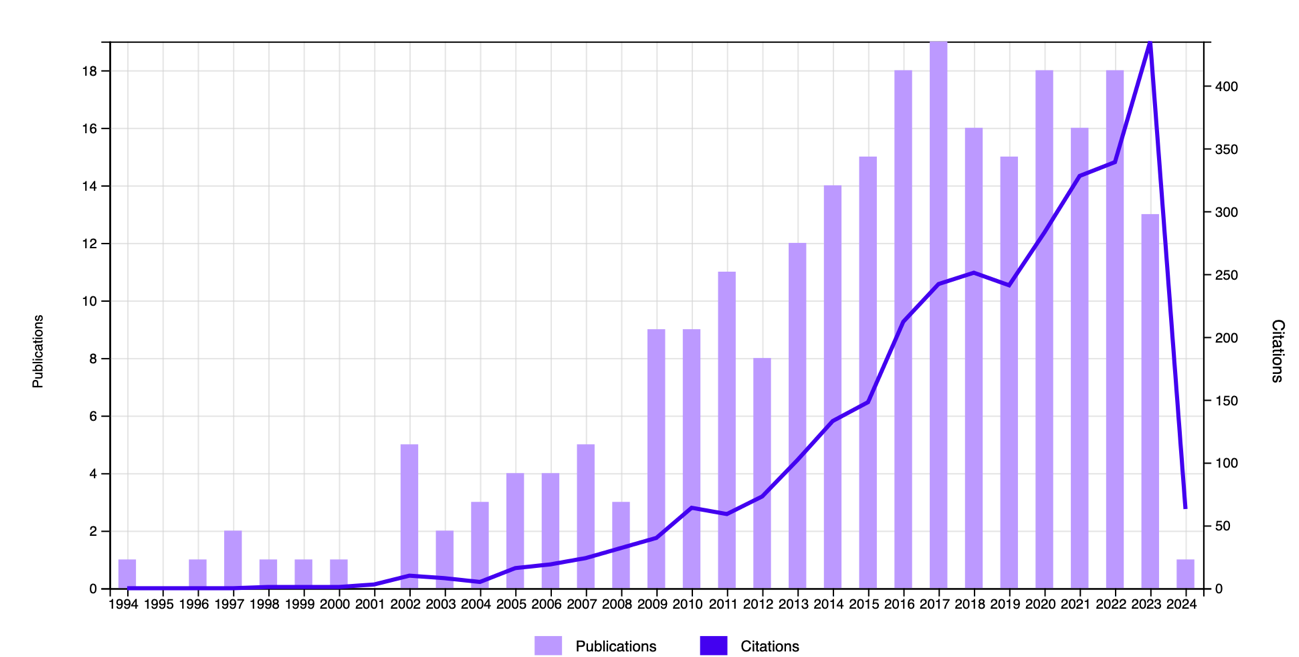
\includegraphics[width=5.90181in,height=2.98425in]{media/image3.png}

Figure 1 -- Web of Science: Citations and publications over time

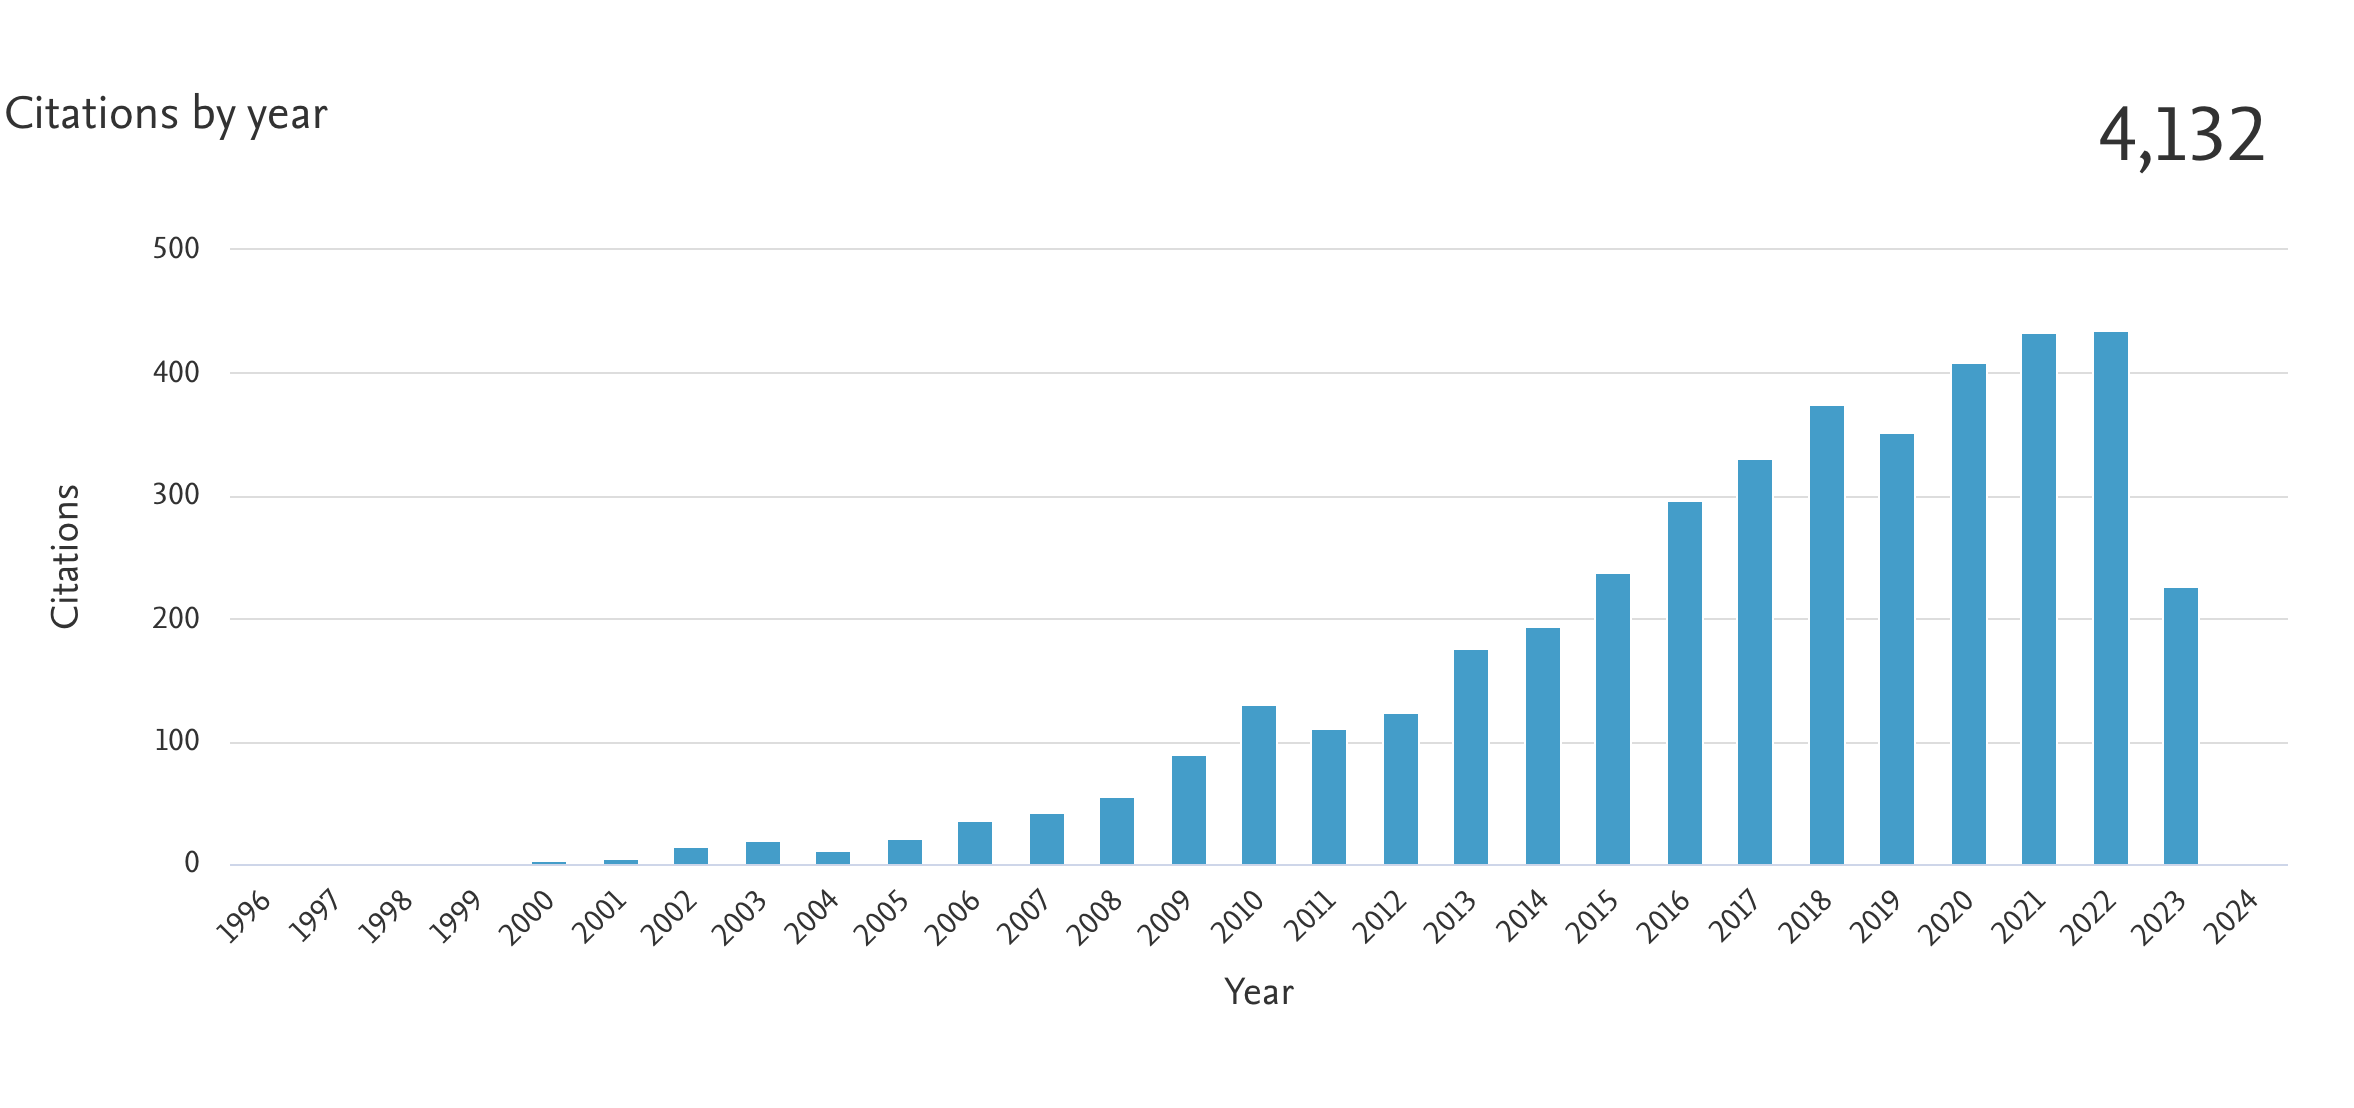
\includegraphics[width=5.75861in,height=2.71024in]{media/image4.png}

Figure 2 -- Scopus : Citations per year

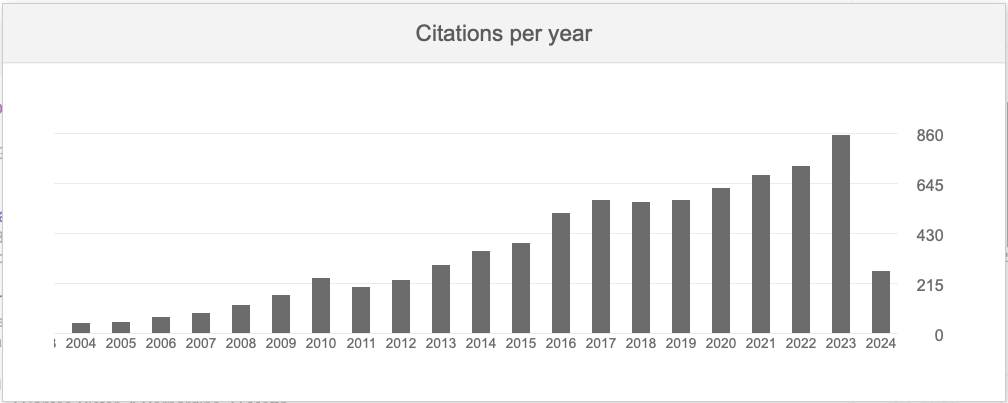
\includegraphics[width=6.06461in,height=2.29217in]{media/image5.png}

Figure 3: Google Scholar: Citations per year.

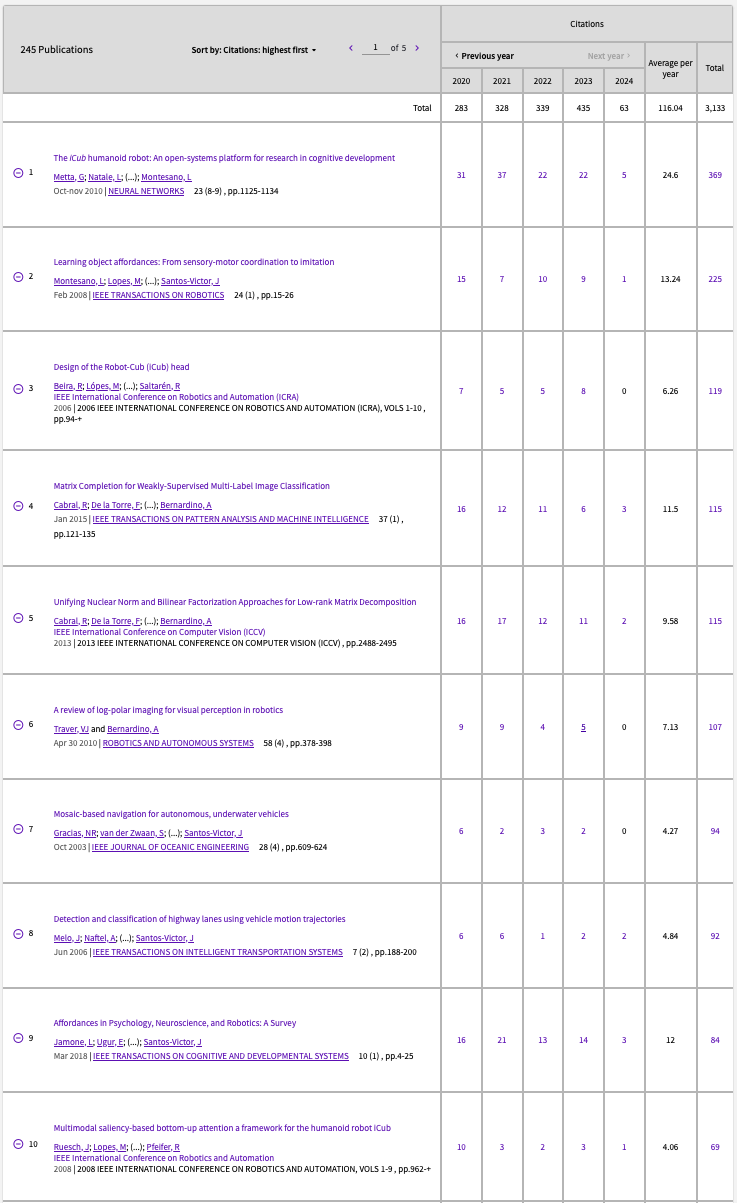
\includegraphics[width=5.76988in,height=9.41831in]{media/image6.png}

Figure 4 -Web of Science : 10 most cited publications.

\subsection{Journal Impact Factors}\label{journal-impact-factors}

Scientific journals are indexed in services that account for several
impact indicators that are typically computed from the number of
citations received by the journal's published articles. Two of the most
renowned journals ranking services are Clarivate Analytics\footnote{Formerly
  known as The Institute for Scientific Information (ISI).} Web of
Science Journal Citation Reports (JCR) and the SCImago Lab's Journal \&
Country Rank (SJR). These services use different types of metrics to
access the relative importance of a journal within its field. Although
there is a large debate about the use of these indexes to assess
scientific work, they carry some value to broadly consider the quality
of the reviewing process in the different journals.

The journals where my papers have been published are listed in Table 2.
For each journal we include the following metrics, when available,
obtained from the Journal Citation Reports (JCR) and the SCImago Journal
Ranks (SJR):

\begin{itemize}
\item
  The 2022 Journal Impact Factor (JIF\footnote{The ratio of the number
    of current year citations to the source items published in that
    journal during the previous two years
    (\url{https://clarivate.com/webofsciencegroup/essays/impact-factor/})})
  obtained from the JCR.
\item
  The 5-Year Journal Impact Factor\footnote{The ratio of the number of
    citations in the previous 5 years to the number of articles
    published in the same period
    (\url{https://clarivate.com/webofsciencegroup/essays/impact-factor/})}
  obtained from JCR.
\item
  The 2022 Journal Citation Index (JCI\footnote{The Journal Citation
    Indicator provides a field-normalized measure of citation impact
    where a value of 1.0 means that, across the journal, published
    papers received a number of citations equal to the average citation
    count in that category
    (\url{https://clarivate.com/wp-content/uploads/dlm_uploads/2021/05/Journal-Citation-Indicator-discussion-paper-2.pdf})}),
  obtained from JCR.
\item
  The categories where the journal is indexed that are most related to
  my research area in JCR and SJR.
\item
  The rank of the journal in each category according to JCR.
\item
  The quartile of the journal in each category according to JCR
  (computed with the JIF or, if not available, the JCI) and SJR
  (computed with the SJR2 indicator\footnote{Vicente P. Guerrero-Bote,
    Félix Moya-Anegón (2012), ``A further step forward in measuring
    journals' scientific prestige: The SJR2 indicator'', Journal of
    Informetrics, 6(4):674-688.}).
\item
  Number of papers I have published in those journals.
\end{itemize}

Whenever the JCR impact factor is not available, the journal ranking
quartiles reported are obtained by JCI, and displayed \emph{in italic
font}.

\begin{longtable}[]{@{}
  >{\raggedright\arraybackslash}p{(\columnwidth - 14\tabcolsep) * \real{0.2667}}
  >{\raggedright\arraybackslash}p{(\columnwidth - 14\tabcolsep) * \real{0.0786}}
  >{\raggedright\arraybackslash}p{(\columnwidth - 14\tabcolsep) * \real{0.0786}}
  >{\raggedright\arraybackslash}p{(\columnwidth - 14\tabcolsep) * \real{0.0785}}
  >{\raggedright\arraybackslash}p{(\columnwidth - 14\tabcolsep) * \real{0.2359}}
  >{\raggedright\arraybackslash}p{(\columnwidth - 14\tabcolsep) * \real{0.1100}}
  >{\raggedright\arraybackslash}p{(\columnwidth - 14\tabcolsep) * \real{0.1100}}
  >{\raggedright\arraybackslash}p{(\columnwidth - 14\tabcolsep) * \real{0.0415}}@{}}
\toprule\noalign{}
\begin{minipage}[b]{\linewidth}\raggedright
\textbf{Journal}
\end{minipage} & \begin{minipage}[b]{\linewidth}\raggedright
\textbf{2022 JIF}
\end{minipage} & \begin{minipage}[b]{\linewidth}\raggedright
\textbf{5-year JIF}
\end{minipage} & \begin{minipage}[b]{\linewidth}\raggedright
\textbf{2022 JCI}
\end{minipage} & \begin{minipage}[b]{\linewidth}\raggedright
\textbf{Category}

\textbf{@}

\textbf{JCR}

\textbf{(SJR)}
\end{minipage} & \begin{minipage}[b]{\linewidth}\raggedright
\textbf{Rank@}

\textbf{JCR categ.}
\end{minipage} & \begin{minipage}[b]{\linewidth}\raggedright
\textbf{Quart}

\textbf{@}

\textbf{JCR}

\textbf{(SJR)}
\end{minipage} & \begin{minipage}[b]{\linewidth}\raggedright
\textbf{\#}
\end{minipage} \\
\midrule\noalign{}
\endhead
\bottomrule\noalign{}
\endlastfoot
Autonomous Robots & 3.5 & 4.6 & 0.72 & Robotics

(Artif. Intel.) & 15/30 & Q2

(Q1) & 2 \\
Drones & 4.8 & 5.5 & 0.92 & Remote Sensing

(Artif. Intel.) & 14/33 & Q2

(Q2) & 1 \\
IEEE Internet of Things Journal & 10.6 & 11.1 & 2.61 & EE Eng.

(Signal Proc.) & 13/275 & Q1

(Q1) & 1 \\
International Journal of Wildland Fire & 3.1 & 3.8 & 1.19 & Forestry

(Forestry) & 13/69 & Q1

(Q1) & 1 \\
User Modeling and User-Adapted Interaction & 3.6 & 5.7 & 0.58 &
Cybernetics

(CS Applic.) & 10/24 & Q2

(Q1) & 1 \\
Informatics & 3.1 & 2.7 & 0.53 & Interdiscipl. App.

(Comp. Networks) & 97/164 & Q3

(Q2) & 1 \\
Expert Systems with Applications & 8.5 & 8.3 & 1.70 & EE Eng.

(Artif. Intel.) & 23/275 & Q1

(Q1) & 1 \\
Remote Sensing & 5.0 & 5.6 & 1.02 & Remote Sensing

(Earth Sciences) & 12/33 & Q2

(Q1) & 3 \\
Frontiers in Robotics and AI & 3.4 & 3.9 & 0.67 & Robotics

(Artif. Intel.) & \emph{23/42} & \emph{Q3}

(Q2) & 4 \\
International Journal of Environmental Research and Public Health & 4.6
& 4.8 & 0.93 & Public Health

(Public Health) & 71/201 & Q2

(Q2) & 1 \\
Sensors & 3.9 & 4.1 & 0.89 & EE Eng.

(EE Eng.) & 100/275 & Q2

(Q2) & 7 \\
Journal of Neuroengineering and Rehabilitation & 5.1 & 5.8 & 1.35 &
Biomedical Eng.

(Health Informatics) & 26/96 & Q2

(Q1) & 1 \\
International Journal of Social Robotics & 4.7 & 4.9 & 1.05 & Robotics

(EE Eng.) & 12/30 & Q2

(Q1) & 3 \\
IEEE Access & 3.9 & 4.1 & 0.89 & EE Eng.

(Engineering) & 100/275 & Q2

(Q1) & 3 \\
Experiments in Fluids & 2.4 & 2.7 & 0.64 & Mechanics

(Comp. Mech.) & 70/133 & Q3

(Q1) & 1 \\
Robotics and Autonomous Systems & 4.3 & 4.6 & 0.84 & Robotics

(Ctr \& Syst. Eng.) & 13/30 & Q2

(Q1) & 9 \\
PLOS Computational Biology & 4.3 & 5.4 & 1.10 & Comp. Biol.

(Mod. \& Sim.) & 10/55 & Q1

(Q1) & 1 \\
Journal of Intelligent \& Robotic Systems & 3.3 & 3.4 & 0.70 & Robotics

(EE Eng.) & 17/30 & Q3

(Q1) & 5 \\
Marine Technology Society Journal & 0.8 & 0.9 & 0.21 & Ocean Eng.

(Ocean Eng.) & 14/16 & Q4

(Q3) & 1 \\
Proceedings of the ACM on Human-Computer Interaction & NA & NA & NA & NA

(HCI) & NA & NA

(Q2) & 1 \\
SoftwareX & 3.4 & 3.3 & 0.88 & Software Eng. & 38/108 & Q2 & 1 \\
Journal of Field Robotics & 8.3 & 7.5 & 1.52 & Robotics

(Ctr \& Syst. Eng.) & 5/30 & Q1

(Q1) & 1 \\
IEEE Robotics and Automation Letters & 5.2 & 5.9 & 1.23 & Robotics

(Ctr \& Syst. Eng.) & 10/30 & Q2

(Q1) & 4 \\
IEEE Transactions on Cognitive and Developmental Systems & 5.0 & 4.8 &
1.13 & Robotics

(Artif. Intel.) & 11/30 & Q2

(Q1) & 3 \\
International Journal of Robotics Research & 9.2 & 9.6 & 1.80 & Robotics

(EE Eng.) & 4/30 & Q1

(Q1) & 1 \\
IEEE Transactions on Circuits and Systems for

Video Technology & 8.4 & 7.1 & 1.89 & EE Eng.

(EE Eng.) & 25/275 & Q1

(Q1) & 1 \\
ACM Computing Surveys & 16.6 & 18 & 4.16 & Comp. Science

(Comp. Science) & 3/111 & Q1

(Q1) & 1 \\
IEEE Transactions

on Geoscience and Remote Sensing & 8.2 & 8.8 & 1.9 & EE Eng.

(EE Eng.) & 27/275 & Q1

(Q1) & 1 \\
Paladyn Journal of Behavioural Robotics & NA & NA & NA & NA

(Artif. Intel.) & NA & NA

(Q3) & 1 \\
Advanced Robotics & 2 & 2.6 & 0.46 & Robotics

(Ctr \& Syst. Eng.) & 26/30 & Q4

(Q2) & 1 \\
International Journal of Advanced Robotic

Systems & 2.3 & 2.3 & 0.41 & Robotics

(Artif. Intel.) & 24/30 & Q4

(Q3) & 2 \\
IEEE Transactions on Magnetics & 2.1 & 2.0 & 0.46 & EE Eng.

(EE Eng.) & 179/275 & Q3

(Q2) & 1 \\
Mechanism and Machine Theory & 5.2 & 5.2 & 1.37 & Mechanical Eng.

(CS Applic.) & 19/135 & Q1

(Q1) & 1 \\
Pattern Recognition & 8.0 & 8.4 & 1.66 & Artif. Intel.

(Artif. Intel.) & 25/145 & Q1

(Q1) & 1 \\
IEEE Transactions on

Systems, Man and Cybernetics : Systems & 8.7 & 9.5 & 2.18 & Aut. \& Ctr.
Systems

(EE Eng.) & 6/65 & Q1

(Q1) & 1 \\
IEEE Robotics \& Automation Magazine & 5.7 & 6.4 & 1.04 & Autom. \& Ctr.
Syst.

(Ctr. \& Syst. Eng.) & 15/65 & Q1

(Q1) & 1 \\
Methods of

Information in Medicine & 1.7 & 2.5 & 0.4 & Information Systems

(Health Informatics) & 128/158 & Q4

(Q3) & 1 \\
Computer Vision and Image Understanding & 4.5 & 5.2 & 0.98 & Artif.
Intel.

(CV \& PR) & 62/145 & Q2

(Q1) & 1 \\
International Journal of Pattern Recognition and Artificial Intelligence
& 1.5 & 1.4 & 0.23 & Artif. Intel.

(Artif. Intel.) & 126/145 & Q4

(Q3) & 1 \\
Pattern Recognition Letters & 5.1 & 4.8 & 0.87 & Artif. Intel.

(Artif. Intel.) & 52/145 & Q2

(Q1) & 2 \\
Neurocomputing & 6.0 & 6.0 & 1.01 & Artif. Intel

(Artif. Intel.) & 41/145 & Q2

(Q1) & 2 \\
IEEE Transactions on Pattern Analysis and Machine Intelligence & 23.6 &
26.7 & 6.76 & Artif. Intel.

(Artif. Intel.) & 2/145 & Q1

(Q1) & 1 \\
International Journal of Machine Intelligence and Sensory Signal
Processing & NA & NA & NA & NA

(NA) & NA & NA

(NA) & 1 \\
Adaptive Behavior & 1.6 & 1.5 & 0.54 & Artif. Intel.

(Artif. Intel.) & 124/145 & Q4

(Q3) & 1 \\
IEEE Transactions on Autonomous Mental Development (2017) & 2.9 & 2.16 &
NA & Artif. Intel.

(NA) & 30/132 & Q1

(NA) & 1 \\
IEEE Transactions on Systems, Man, and Cybernetics, Part B: Cybernetics
(2014) & 6.2 & 6.2 & NA & Autom. \& Ctr. Syst.

(Ctr. \& Syst. Eng.) & 2/58 & Q1

(Q1) & 1 \\
Machine Vision and Applications & 3.3 & 2.6 & 0.54 & EE Eng.

(CV \& PR) & 114/275 & Q2

(Q2) & 1 \\
Neural Networks & 7.8 & 8.4 & 1.58 & Artif. Intel.

(Artif. Intel.) & 28/145 & Q1

(Q1) & 1 \\
IEEE Transactions on Robotics and Automation (2004) & 2.1 & NA & NA &
Autom. \& Ctr. Syst.

(Ctr. \& Syst. Eng.) & 2/46 & Q1

(Q1) & 1 \\
IEEE Transactions on Robotics & 7.8 & 10.2 & 1.79 & Robotics

(Ctr. \& Syst. Eng.) & 7/30 & Q1

(Q1) & 1 \\
IEEE Transactions on Image Processing & 10.6 & 13.3 & 2.01 & Artif.
Intel.

(Software) & 13/145 & Q1

(Q1) & 1 \\
IEEE Transactions on Intelligent Transportation Systems & 8.5 & 9.0 &
2.18 & EE Eng.

(CS Applic.) & 23/275 & Q1

(Q1) & 1 \\
IEEE Journal of Oceanic Engineering & 4.1 & 4.2 & 1.17 & EE Eng.

(EE Eng.) & 97/275 & Q2

(Q1) & 1 \\
\end{longtable}

\clearpage
\section{Project Grants}\label{project-grants}

On the description of the funding, for each project I show both the
global budget and the budget for the participating institution, in the
format (global budget / local budget).

\subsection{Project Grants as Global
Coordinator}\label{project-grants-as-global-coordinator}

\begin{enumerate}
\def\labelenumi{\arabic{enumi}.}
\item
  \ul{HAVATAR}
\end{enumerate}

Title: Healthcare Added-Value Applications of Tele-Autonomous Robots

Dates: 2021-03-01 to 2024-02-28 (successfully concluded)

Reference: \url{https://doi.org/10.54499/PTDC/EEI-ROB/1155/2020}

Funding: FCT (248K€ / 130K€)

\begin{quote}
Institutions: \emph{Instituto de Sistemas e Robótica, IST-ID}

\emph{Instituto de Sistemas e Robótica -- Universidade de Coimbra}

\emph{Hospital da Luz GLSMED Learning Health, S.A.}
\end{quote}

Role: Global Coordinator (Principal Investigator)

\begin{quote}
Abstract: The HAVATAR project developed new software skills for
telepresence robots that increase their level of autonomy, the
teleoperation comfort of the user, and its social presence at the remote
site. Two academic partners with long-standing international experience
in robotics projects (IST-ID Lisboa and ISR-UC Coimbra) will collaborate
for the development of the tele-autonomy skills and their integration in
the healthcare added-value applications, that will be tested in
realistic scenarios provided by Hospital da Luz Learning Health (HL.LH).
One application will be hosted at the HL.LH Simulation Center, where
practitioner students, health professionals or other actors will
remotely access a telepresence robot to dynamically observe simulated
clinical practices and interact with the local peers (e.g. simulated
surgical acts or simulated Intensive Care Unit in a pandemic scenario).
In this scenario, we will also study the issue of having multiple remote
users sharing the same local space and interacting with each other via
their proxy robots. The other application will deploy one telepresence
robot in the home of a patient and let the relatives or health
professionals interact and program the robot to acquire added value
variables and patient reported data. In this application, we will study
how extended periods of autonomy can be useful for healthcare
professionals.
\end{quote}

\begin{enumerate}
\def\labelenumi{\arabic{enumi}.}
\setcounter{enumi}{1}
\item
  \ul{FIREFRONT}
\end{enumerate}

\begin{quote}
Title: Real­-Time Forest Fire Mapping and Spread Forecast Using Unmanned
Aerial Vehicles
\end{quote}

Dates: 2019-03-01 to 2023-02-28 (successfully concluded)

Funding: FCT with reference PCIF/SSI/0096/2017 (377K€ / 102K€)

\begin{quote}
Institutions: \emph{Instituto de Sistemas e Robótica, IST-ID}

\emph{Aeroclube de Torres Vedras - Centro de Ciência do Ar e do Espaço}

\emph{Associação para o Desenvolvimento da Aerodinâmica Industrial}

\emph{Força Aérea Portuguesa}

\emph{Instituto de Telecomunicações}

\emph{UAVision, Engenharia de Sistemas, Ltd}
\end{quote}

Role: Global Coordinator (Principal Investigator)

\begin{quote}
Abstract: This project develops solution to support firefighting actions
in forest fires through the real­time detection and tracking of fire
fronts and re­burns. This is achieved by processing the information
acquired from manned and unmanned aerial vehicles equipped with
specialized sensing and communication systems, that overfly the affected
areas. This information can be made available to the coordination and
fighting units on a graphical interface the localization of the fire
events in georeferenced coordinates. Forecasts of the fire front
evolution, images of the fire area, wind speed and direction, and other
meteorological data of interest can also be supplied. This information
is of great value for decision making on firefighting actions.
\end{quote}

\begin{enumerate}
\def\labelenumi{\arabic{enumi}.}
\setcounter{enumi}{2}
\item
  \ul{VOAMAIS}
\end{enumerate}

\begin{quote}
Title: Computer Vision for the Operation of Unmanned Aerial Vehicles in
Maritime and WildfIre Scenarios
\end{quote}

Dates: 2019-02-01 to 2023-01-31 (successfully concluded)

Funding: FCT with reference PTDC/EEI-AUT/31172/2017 (222K€ / 154K€)

\begin{quote}
Institutions: \emph{Instituto de Sistemas e Robótica, IST-ID}

\emph{Força Aérea Portuguesa}

\emph{Marinha Portuguesa}
\end{quote}

Role: Global Coordinator (Principal Investigator)

\begin{quote}
Abstract: This project developed novel methods for target detection and
tracking in airborne and seaborne image sequences. The availability of
low-cost visual sensors (visible and IR) and the recent developments on
convolutional neural-networks and correlation filters are cost-effective
and energy-efficient solutions for detection and tracking of targets
capable of running onboard on air or sea vehicles. The results of the
project have a direct impact on strategic national activities such as
ocean and forest monitoring. To demonstrate the applicability of the
methods, three case scenarios are considered: (i) detection of forest
fires from airborne images, (ii) detection and tracking of sea vessels
from airborne and seaborne images, and (iii) detection, tracking and
pose estimation of aircrafts from seaborne images for teleguidance of
unmanned aerial vehicles (UAV's). These demonstrations will inform the
responsible institutions for the protection of the environment and
coastal operations of a novel technology to support their activities.
\end{quote}

\begin{enumerate}
\def\labelenumi{\arabic{enumi}.}
\setcounter{enumi}{3}
\item
  \ul{AHA}
\end{enumerate}

\begin{quote}
Title: Augmented Human Assistance
\end{quote}

Dates: 2014-08-01 to 2018-12-31 (successfully concluded)

Funding: FCT with reference CMUP-ERI/HCI/0046/2013 (590K€/307K€)

\begin{quote}
Institutions: \emph{Instituto de Sistemas e Robótica, IST-ID}

\emph{Faculdade de Motricidade Humana}, \emph{Universidade de Lisboa}

\emph{Madeira Interactive Technologies Institute M-ITI}

\emph{NOVA.ID.FCT}

\emph{PLUX, Engenharia de Biosensores, Lda}.

\emph{YDreams - Informática, SA}

\emph{Carnegie Mellon University} (US)
\end{quote}

Role: Global Coordinator (Principal Investigator)

\begin{quote}
Abstract: This project is a novel, integrative and cross-disciplinar
approach of 4 portuguese universities, CMU and 2 portuguese industry
partners that combines innovation and fundamental research in the areas
of human computer interaction, robotics, serious games and physiological
computing. AHA has developed a new generation of ICT based solutions
that have the potential to transform healthcare by optimizing resource
allocation, reducing costs, improving diagnoses and enabling novel
therapies, thus increasing quality of life. The project proposes the
development and deployment of a novel Robotic Assistance Platform
designed to support healthy lifestyle, sustain active aging, and support
those with motor deficits.
\end{quote}

\begin{enumerate}
\def\labelenumi{\arabic{enumi}.}
\setcounter{enumi}{4}
\item
  \ul{LIMOMAN}
\end{enumerate}

\begin{quote}
Title: Developmental Learning of Internal Models for Robotic
Manipulation based on Motor Primitives and Multisensory Integration
\end{quote}

Dates: 2014-05-01 to 2016-04-30 (successfully concluded)

Funding: EU-FP7-PEOPLE-2013-IEF, grant agreement 628315 (147K€)

\begin{quote}
Institutions: \emph{Instituto de Sistemas e Robótica, Instituto Superior
Técnico}
\end{quote}

Role: Global Coordinator

\begin{quote}
Abstract: LIMOMAN (developmental Learning of Internal MOdels for robotic
MANipulation based on motor primitives and multisensory integration)
addresses the key problem of improving the ability of current robots in
dexterous manipulation, inspired by three main aspects of the human
motor control system: internal models, learning and multisensory
integration. Internal models that encode the robot sensorimotor
capabilities and the dynamics of its interaction with the environment
are exploited to generate predictions that improve both robot perception
and motion control. These models are either acquired from scratch and/or
progressively refined and adapted through learning and optimization
techniques, using sensorimotor data collected by the robot during
goal-directed actions. The combination of different sensory modalities
(vision, proprioception, touch) and the use of probabilistic (Bayesian)
techniques permits to achieve robot behaviors that are effective, robust
and safe.
\end{quote}

\begin{enumerate}
\def\labelenumi{\arabic{enumi}.}
\setcounter{enumi}{5}
\item
  \ul{BIOMORPH}
\end{enumerate}

\begin{quote}
Title: Bio-inspired self-organizing robot computational morphologies
\end{quote}

Dates: 2014-02-01 to 2015-07-31 (successfully concluded)

Funding: FCT with reference EXPL/EEI-AUT/2175/2013 (49K€)

\begin{quote}
Institutions: \emph{Instituto de Sistemas e Robótica, IST-ID}
\end{quote}

Role: Coordinator (Principal Investigator)

\begin{quote}
Abstract: This project progressed towards the development of highly
efficient, scalable and adaptable control structures for autonomous
robotic agents, using biological principles for the creation of sparse
sensorimotor couplings and prediction mechanisms. The developed methods
were implemented and tested in concrete robotic test beds to prove the
proposed concepts in realistic scenarios and compared them with more
classical control approaches.
\end{quote}

\begin{enumerate}
\def\labelenumi{\arabic{enumi}.}
\setcounter{enumi}{6}
\item
  \ul{BIOLOOK}
\end{enumerate}

\begin{quote}
Title: Biomimetic Oculomotor Control for Humanoid Robots
\end{quote}

Dates: 2007-10-01 to 2010-11-30 (successfully concluded)

Funding: FCT with reference FCT - PTDC/EEA-ACR/71032/2006 (90K€)

\begin{quote}
Institutions: \emph{Instituto de Sistemas e Robótica, IST-ID}

\emph{University of Uppsala} (SW)
\end{quote}

Role: Global Coordinator (Principal Investigator)

\begin{quote}
Abstract: In this project we addressed the following scientific topics
in oculomotor control: (i) how to perform human-like eye-head movements
and postures in the execution of tasks and interaction with humans; (ii)
how oculomotor processes are learned and developed through childhood,
and how can be exploited to create adaptive autonomous systems; and
(iii) how robot behaviour can be modulated to implicitly communicate
emotions, intentions and goals to human users. The studied methodologies
were implemented and tested both in realistic dynamical simulations and
in prototype humanoid robotic platforms available in the consortium.
\end{quote}

\begin{enumerate}
\def\labelenumi{\arabic{enumi}.}
\setcounter{enumi}{7}
\item
  \ul{FOVEAR}
\end{enumerate}

\begin{quote}
Title: Foveal Vision for Robotics Applications
\end{quote}

Dates: 2006-04-01 to 2008-03-31 (successfully concluded)

Funding: FCT (Luso-Spain Integrated Action) with reference E-47/06 (4K€)

\begin{quote}
Institutions: \emph{Instituto de Sistemas e Robótica, Instituto Superior
Técnico}

\emph{Universidad Jaume I, Castellon de la Plana}
\end{quote}

Role: Principal Investigator

\begin{quote}
Abstract: The FOVEAR Project developed computer vision technology for
robotics applications with foveal vision sensors. These sensors yield a
significant reduction of the amount of information to process at any
time, while still allowing wide fields of view and high acuity in the
center of the visual field, like in the human retina. This allows the
real-time operation of robotic systems in generic and unconstrained
environments.
\end{quote}

\subsection{Project Grants As Coordinator of Participating
Institution}\label{project-grants-as-coordinator-of-participating-institution}

\begin{enumerate}
\def\labelenumi{\arabic{enumi}.}
\item
  \ul{ORIENT}
\end{enumerate}

\begin{quote}
Title: Goal-directed eye-head coordination in dynamic multisensory
environment.
\end{quote}

Dates: 2019-07-01 to 2022-12-31 (successfully concluded)

Reference: \url{https://doi.org/10.3030/693400}

Funding: H2020-EU.1.1, ERC-215-AdG, n. 693400 (2523K€/314K€)

\begin{quote}
Institutions: \emph{Stichting Radboud Universiteit, Nijmegen} (NL)

\emph{Instituto de Sistemas e Robótica, Instituto Superior Técnico}

\emph{Instituto de Sistemas e Robótica, IST-ID}
\end{quote}

Role: Participating Institution Coordinator

\begin{quote}
Abstract: Rapid object identification is crucial for survival of all
organisms but poses daunting challenges if many stimuli compete for
attention, and multiple sensory and motor systems are involved in the
processing, programming and generating of an eye-head gaze-orienting
response to a selected goal. How do normal and sensory-impaired brains
decide which signals to integrate (``goal''), or suppress
(``distracter'')? Audiovisual (AV) integration only helps for spatially
and temporally aligned stimuli. However, sensory inputs differ markedly
in their reliability, reference frames, and processing delays, yielding
considerable spatial-temporal uncertainty to the brain. Vision and
audition utilize coordinates that misalign whenever eyes and head move.
Meanwhile, their sensory acuities vary across space and time in
essentially different ways. As a result, assessing AV alignment poses
major computational problems, which so far have only been studied for
the simplest stimulus-response conditions.
\end{quote}

\begin{enumerate}
\def\labelenumi{\arabic{enumi}.}
\setcounter{enumi}{1}
\item
  \ul{ELEVAR}
\end{enumerate}

\begin{quote}
Title: Study of Vertical Structures with Robotized Aircrafts
\end{quote}

Dates: 2017-04-01 to 2019-03-31 (successfully concluded)

Funding: PT2020 - LISBOA-01-0247-FEDER-17924 (101K€)

\begin{quote}
Institutions: \emph{Tekever ASDS Lda}

\emph{Instituto de Sistemas e Robótica, Instituto Superior Técnico}

\emph{Laboratório Nacional de Engenharia Civil}
\end{quote}

Role: Participating Institution Coordinator

\begin{quote}
Abstract: The inspections and assessments of the structural integrity of
large infrastructures (eg. dams, bridges and high voltage cables) are
inadequate because they are not performed in a systematic manner and
they greatly depend on the personal criteria of the inspection
engineers. Additionally, certain areas of these structures or difficult
to reach by conventional means and the locations where data can be
acquired are limited which in turn can compromise the quality of the
gathered information and make these inspections costly. Some of the
already existing solutions based on multicopters are completely
dependent on a certified operator and/or GPS, lacking the ability to
perform an autonomous survey without the support of an infrastructure
that supplies the platform with global positioning signals. The solution
proposed by ELEVAR consists of utilizing an autonomous unmanned aircraft
integrated with sensors and vision-based navigation algorithms to solve
the above-mentioned problems.
\end{quote}

\begin{enumerate}
\def\labelenumi{\arabic{enumi}.}
\setcounter{enumi}{2}
\item
  \ul{iPEPE}
\end{enumerate}

\begin{quote}
Title: Cognitive Rehabilitation with Portable Exergame Platforms for the
Elderly
\end{quote}

Dates: 2020-06-01 to 2023-05-31 (successfully concluded)

Funding: P2020 with reference LISBOA-06-4234-FSE-000079 (30K€ / 74K€)

\begin{quote}
Institutions: \emph{Instituto das Irmãs Hospitaleiras do Sagrado Coração
de Jesus}

\emph{Instituto de Sistemas e Robótica, Instituto Superior Técnico}
\end{quote}

Role: Participating Institution Coordinator

\begin{quote}
Abstract: This project developed and tested augmented reality exergames
for the cognitive stimulation of the elder people living in nursing
homes or care institutions. These games put together physical and
cognitive tasks in entertaining and motivating activities and have been
shown to have benefits at the physical, cognitive, and social
dimensions. In this project a special attention is given to patient with
dementia, to assess if the proposed approach can be applied to this
fraction of the population.
\end{quote}

\begin{enumerate}
\def\labelenumi{\arabic{enumi}.}
\setcounter{enumi}{3}
\item
  \ul{SEAGULL}
\end{enumerate}

\begin{quote}
Title: Intelligent Systems for the Maritime Situational Awareness using
Unmanned Aerial Vehicles.
\end{quote}

Dates: 2013-07-01 to 2015-06-30 (successfully concluded)

Funding: QREN - FCOMP-01-0202-FEDER-034063 (870K€/97K€)

\begin{quote}
Institutions: \emph{Critical Software, SA}

\emph{Instituto de Sistemas e Robótica, Instituto Superior Técnico}

\emph{Faculdade de Engenharia da Universidade do Porto}

\emph{Força Aérea Portuguesa}

\emph{Marinha Portuguesa}
\end{quote}

Role: Participating Institution Coordinator

\begin{quote}
Abstract: Portugal is a maritime nation having the largest exclusive
economic zone (EEZ) of Europe. Upon acceptance of the proposal submitted
to the United Nations (UN), the Portuguese EEZ will be extended to an
area larger than 2 million square kilometres. In addition, Portugal is
known as a specialist in maritime matters not only by historical reasons
but also due to its contemporary activities on the sea. It is crucial
for Portugal to maintain the safety of human life at sea, maintain the
safety of its maritime area, and protect the sea and coastline natural
environments. The SEAGULL project consists on the use of unmanned air
vehicles (UAV's) as a not only viable but also cheaper solution to help
with these difficult tasks on such a large area. The objective is to
develop an intelligent system that couples the UAV with sensors like
visual, infra-red and hyperspectral cameras along with GPS receivers and
other sensors. Its purpose is to fly autonomously over the sea while
scanning it to automatically detect, identify, report and follow targets
like boats, shipwrecks, lifeboats, boats with suspicious behaviour, and
also hydrocarbyls and other chemical pollutants.
\end{quote}

\begin{enumerate}
\def\labelenumi{\arabic{enumi}.}
\setcounter{enumi}{4}
\item
  \ul{DICO(RE)2S}
\end{enumerate}

\begin{quote}
Title: Discount Coupon Recommendation and Redemption System
\end{quote}

Dates: 2011-07-01 to 2016-06-30 (successfully concluded)

Funding: EU-FP7-SME-262451 (1428K€/216K€)

\begin{quote}
Institutions: \emph{Fundacio Barcelona Media} (ES)

\emph{Nova Ventus Consulting SL} (ES)

\emph{Nextage SRL} (IT)

\emph{Aitek SPA} (IT)

\emph{Observit -- Tecnologias de Visão por Computador, Lda}

\emph{Instituto de Sistemas e Robótica, Instituto Superior Técnico}
\end{quote}

Role: Participating Institution Coordinator

\begin{quote}
Abstract: DICO(RE)2S is an SME European Consortium devoted to develop
and deploy a coupon-based discount campaign platform that will exploit
state-of-the-art information and communication technologies and
processes for providing consumers and retailers/manufactures with a
personalized and efficient environment for maximizing customer
satisfaction and business profitability. The distributed network of
coupon redemption points will implement pattern recognition systems for
reading and validating coupons as well as security encryption and
transmission systems that will guarantee the integrity of the overall
coupon redemption strategy as well as the reliability of the data.
\end{quote}

\begin{enumerate}
\def\labelenumi{\arabic{enumi}.}
\setcounter{enumi}{5}
\item
  \ul{HDA}
\end{enumerate}

\begin{quote}
Title: High-Definition Analytics.
\end{quote}

Dates: 2010-05-01 to 2013-10-30 (successfully concluded)

Funding: QREN - FCOMP-01-0202-FEDER-013750 (536K€/203K€)

\begin{quote}
Institutions: \emph{Observit -- Tecnologias de Visão por Computador,
Lda}

\emph{Instituto de Sistemas e Robótica, Instituto Superior Técnico}
\end{quote}

Role: Participating Institution Coordinator and Global Scientific
Coordinator

\begin{quote}
Abstract: HD-Analytics is a QREN research project aimed at the
development of new algorithms and methods to address important video
analytics challenges, in the context of new technology available in the
IP camera market: high-resolution multi-megapixel cameras and
high-resolution omni-directional cameras. Thus, new algorithms and
methods are required to deal with the increased amount of data.
\end{quote}

\begin{enumerate}
\def\labelenumi{\arabic{enumi}.}
\setcounter{enumi}{6}
\item
  \ul{HANDLE}
\end{enumerate}

\begin{quote}
Title: Developmental pathway towards autonomy and dexterity in robot
in-hand manipulation
\end{quote}

Dates: 2009-02-01 to 2013-01-31 (successfully concluded)

Funding: EU-FP7-ICT-231640 (8190K€/749K€)

\begin{quote}
Institutions: \emph{Universite Pierre et Marie Curie, Paris 6} (FR)

\emph{Universitaet Hamburg} (DE)

\emph{Universidad Carlos III de Madrid} (ES)

\emph{Commissariat a L'Energie Atomique et Aux Energies Alteratives}
(FR)

\emph{Instituto de Sistemas e Robótica, Instituto Superior Técnico}

\emph{Faculdade de Ciências e Tecnologia da Universidade de Coimbra}

\emph{Orebro University} (SW)

\emph{Kings College London} (UK)

\emph{The Shadow Robot Company Limited} (UK)
\end{quote}

Role: Participating Institution Coordinator and Global Technical Manager

\begin{quote}
Abstract: The HANDLE project aims at understanding how humans perform
the manipulation of objects to replicate grasping and skilled in-hand
movements with an anthropomorphic artificial hand, and thereby move
robot grippers from current best practice towards more autonomous,
natural, and effective articulated hands. The project implies not only
focusing on technological developments but also working with fundamental
multidisciplinary research aspects to endow the robotic hand system with
advanced perception capabilities, high level feedback control and
elements of intelligence that allow recognition of objects and context,
reasoning about actions and a high degree of recovery from failure
during the execution of dexterous tasks.
\end{quote}

\begin{enumerate}
\def\labelenumi{\arabic{enumi}.}
\setcounter{enumi}{7}
\item
  \ul{VEMUCARV}
\end{enumerate}

\begin{quote}
Title: Spatial Validation of Complex Urban Grids in Virtual Imersive
Environments
\end{quote}

Dates: 2009-02-01 to 2013-01-31 (successfully concluded)

Funding: FCT - POCTI/AUR/48123/2002 (25K€)

\begin{quote}
Institutions: \emph{Institute of Mechanical Engineering, Instituto
Superior Técnico}

\emph{Instituto de Sistemas e Robótica, Instituto Superior Técnico}

\emph{Câmara Municipal de Lisboa}
\end{quote}

Role: Participating Institution Coordinator

\begin{quote}
Abstract: The main goals of this project are related to the
semi-automatic acquisition and maintenance of 3D virtual reality models
of urban areas. It is intended to use registered aerial images and low
altitude laser range scans to acquire 3D data of city structure. This
data will be processed in order to segment relevant structures for urban
planning (buildings, roads, green areas, etc). Range information
provides a very rich description of 3D structure but lack photometric
information. Aerial photos provide this information, allowing to
pre-segment regions based on color and texture. The main scientific
innovation of this project is the combined use of 2D (aerial images) and
3D (range scans) to simplify and improve the building extraction
process. Most current approaches use one or the other types of data
exclusively. The final result provides a computer model which stands for
a mix geometry-image database that can interface to GIS software
available (at CML), as well as the generation of real-time walkthrough
with thematic information. The results of this project are to be
integrated on Lisbon City Hall public computational facilities.
\end{quote}

\subsection{Project Grants As Team
Member}\label{project-grants-as-team-member}

\begin{enumerate}
\def\labelenumi{\arabic{enumi}.}
\item
  \ul{RePAIR}
\end{enumerate}

\begin{quote}
Title: Reconstructing the Past: Artificial Intelligence and Robotics
Meet Cultural Heritage
\end{quote}

Dates: 2021-06-01 to 2024-11-30 (ongoing)

Funding: H2020 FETOPEN - Grant agreement 964854 (3522K€/575K€)

\begin{quote}
Institutions: \emph{Universita Ca'Foscari, Venezia} (IT)

\emph{Instituto de Sistemas e Robótica, IST-ID}

\emph{Ben-Gurion University of the Negev} (IR)

\emph{Fondazione Istituto Italiano di Tecnologia} (IT)

\emph{Rheinische Friedrich-Wilhelms-Universitat Bonn} (DE)

\emph{Ministero Della Coltura} (IT)
\end{quote}

Role: Team Member

\begin{quote}
Abstract: The physical reconstruction of shattered artworks is one of
the most labour-intensive steps in archaeological research. Dug out from
excavation sites are countless ancient artefacts, such as vases,
amphoras and frescoes, that are damaged. The EU-funded RePAIR project
will facilitate the reconstruction process to bring ancient artworks
back to life. Specifically, it will develop an intelligent robotic
system that can autonomously process, match and physically assemble
large fractured artefacts in a fraction of the time required by humans.
This new system will be tested on iconic case studies from the UNESCO
World Heritage Site of Pompeii. It will restore two world-renowned
frescoes, which are in thousands of broken pieces and currently in
storerooms.
\end{quote}

\begin{enumerate}
\def\labelenumi{\arabic{enumi}.}
\setcounter{enumi}{1}
\item
  \ul{ShiftHRI}
\end{enumerate}

\begin{quote}
Title: Exploring the Transfer of Agency to Older Adults in HRI
\end{quote}

Dates: 2022-03-01 to 2023-05-28 (successfully concluded)

Funding: FCT, CMU/TIC/0026/2021 (63K€/26K€)

\begin{quote}
Institutions: \emph{LASIGE}

\emph{Instituto de Sistemas e Robótica, IST-ID}

\emph{Carnegie Mellon University} (US)
\end{quote}

Role: Team Member

\begin{quote}
Abstract: Our vision is to advance research on human-robot interaction
to facilitate a new type of relationship between elders and assistive
robots. This relationship will be built on a deep understanding of human
values and what is critical to older adults. Our previous work shows
that values are manifested through interactions with products, and that
this becomes more critical for elders as they experience physical,
cognitive, and emotional decline. In addition, what elders value can
change dynamically, even day to day, as elders experience decline. In
ShiftHRI, we will start by exploring important values and co-designing
HRI scenarios that help people to fulfil them. This paradigm shift has
the potential to significantly impact the research done in the area.
Contrary to the state of the art, where most robots have strict
predefined user interfaces and routines, shifting agency to older adults
brings several challenges to the control of those robots and in the
service they offer.
\end{quote}

\begin{enumerate}
\def\labelenumi{\arabic{enumi}.}
\setcounter{enumi}{2}
\item
  \ul{IntelligentCare}
\end{enumerate}

\begin{quote}
Title: Intelligent Multimorbidity Management System
\end{quote}

Dates: 2020-04-01 to 2023-06-30 (successfully concluded)

Funding: LISBOA-01-0247- FEDER-045948 (3522K€/497K€)

\begin{quote}
Institutions: \emph{GLSMED Learning Health S.A.}

\emph{Instituto de Sistemas e Robótica, Instituto Superior Técnico}

\emph{Instituto de Sistemas e Robótica, IST-ID}

\emph{Hospital da Luz S.A.}

\emph{Instituto De Engenharia De Sistemas E Computadores, Investigação e
Desenvolvimento Em Lisboa}

\emph{Priberam Informática S.A.}

\emph{Carnegie Mellon University} (US)
\end{quote}

Role: Team Member

\begin{quote}
Abstract: This project focus on managing the issue of a growing
population with multimorbidity (co-occurring diseases), a worldwide
problem to the sustainability of the healthcare system. IntelligentCare
aims to develop a patient-centric solution to manage multimorbidity
conditions by using analytical methods to explore data from the
electronic health records and measures reported remotely by the
patients. Under the value-based healthcare framework, the project will
develop methods for early signalization and characterization of
patients, identification of personalized clinical pathways based on
evidence, and based on patient value vision, together with monitoring
and prediction of hospital interactions. To achieve these goals research
will be conducted in advanced analytical algorithms, particularly deep
learning methods, to fully explore data. This is an innovative approach
to evaluate the multimorbidity condition by introducing the concept of
value to the patient in the process of characterization and prediction
of patient interactions with the hospital.
\end{quote}

\begin{enumerate}
\def\labelenumi{\arabic{enumi}.}
\setcounter{enumi}{3}
\item
  \ul{ASTRIIS}
\end{enumerate}

\begin{quote}
Title: Atlantic Sustainability Through Remote and In-situ Integrated
Solutions

Dates: 2020-03-01 to 2023-06-30 (successfully concluded)

Funding: POCI-01-0247-FEDER-046092 (891K€/273K€)

Institutions: \emph{Tekever}

\emph{+Atlantic CoLAB}

\emph{CEiiA}

\emph{Hidromod, modelação em engenharia}

\emph{Institute for Systems and Robotics, IST}

\emph{ISQ}

\emph{LSTS, Underwater Systems and Technology Laboratory, FEUP}

\emph{MARETEC, Marine Environment and Technology Center, IST}

\emph{CERENA, Center of Natural Resources and Environment, IST}

\emph{Ocean Infinity}

\emph{Ocean Scan, Marine Systems \& Technology Lda}

\emph{Spin.Works, S.A.}

\emph{WavEC Offshore Renewables}

\emph{Universidade do Minho}

\emph{Universidade do Algarve}

Role: Team Member

Abstract: This project is a Portuguese effort to support the sustainable
growth of the blue economy by developing technical and scientific
knowledge for the design, demonstration and implementation of integrated
and customizable information products and services. The project focuses
on sectors of the blue economy with high potential for value creation,
such as marine renewable energy, aquaculture, coastal tourism, or
recreational boating, and is oriented to the needs of users, which
include investors, regulators, policymakers, consumers, and scientific
researchers. The ISR team participated in the development of remote
sensing solutions for environmental monitoring of the Atlantic national
coastal waters.
\end{quote}

\begin{enumerate}
\def\labelenumi{\arabic{enumi}.}
\setcounter{enumi}{4}
\item
  \ul{RBCog-Lab}
\end{enumerate}

\begin{quote}
Title: Robotics, Brain and Cognition Lab
\end{quote}

Dates: 2017-06-01 to 2021-11-30 (successfully concluded)

\begin{quote}
Funding: FCT - Portuguese Roadmap of Research Insfrastructures
01/SAICT/2016 SAICT Proj. 22084 (300K€)

Institutions: \emph{Instituto de Sistemas e Robótica, Instituto Superior
Técnico}

\emph{Instituto de Sistemas e Robótica, IST-ID}
\end{quote}

Role: Team Member

\begin{quote}
Abstract: The Robotics, Brain and Cognition Lab (RBCogLab) is part of
the Portuguese Roadmap of Research Infrastructures. RBCog-Lab supports
an integrated multidisciplinary research endeavour (neuroscience,
developmental psychology, cognitive science, psychophysics, machine
learning and other engineering subjects) not only promoting novel
robotic methodologies but also contributing to a better understanding of
the human brain. To be effective and generate a positive impact in the
society, this multidisciplinary research needs to be supported by
advanced equipment and specialized technical expertise, that might not
be available in small research and academic centres with low budgets.
The RBCogLab research infrastructure aims at filling this gap by
providing the scientific community with a centralized open laboratory
resource for robotics experiments and human measurements, offering both
state of the art devices and specialized know-how.
\end{quote}

\begin{enumerate}
\def\labelenumi{\arabic{enumi}.}
\setcounter{enumi}{5}
\item
  \ul{ALHTOUR}
\end{enumerate}

\begin{quote}
Title: Assisted Living Technologies for the Health Tourism Sector
\end{quote}

Dates: 2016-01-01 to 2018-12-31 (successfully concluded)

Funding: H2020-TWINN-2015 Grant Agreement 692311 (1175K€/40K€)

\begin{quote}
Institutions: \emph{Universidade de Lisboa}

\emph{Faculdade de Motricidade Humana}

\emph{Faculdade de Medicina da Universidade de Lisboa}

\emph{Faculdade de Ciências da Universidade de Lisboa}

\emph{Instituto de Ciências Sociais}

\emph{Instituto Superior Técnico}

\emph{Katholieke Universiteit Leuven} (BE)

\emph{Universiteit Maastricht} (NL)

\emph{Universita degli studi di Macerata} (IT)

Role: Coordinator of activities at the Institute for Systems and
Robotics, Instituto Superior Técnico.

Abstract: The ALHTOUR project aims to strengthen and stimulate
scientific excellence, and innovation capacity in technologies for
independent living, applied to the health tourism at UL (Portugal), by
preparing for the set-up of a ``Health Tourism Living Lab'', identified
as a key driver for territorial development.
\end{quote}

\begin{enumerate}
\def\labelenumi{\arabic{enumi}.}
\setcounter{enumi}{6}
\item
  \ul{SPARSIS}
\end{enumerate}

\begin{quote}
Title: Sparse Modeling and Estimation of Motion Fields
\end{quote}

Dates: 2016-07-01 to 2019-12-31 (successfully concluded)

Funding: FCT - PTDC/EEI-PRO/0426/2014 (199K€)

\begin{quote}
Institutions: \emph{Instituto de Sistemas e Robótica, Associação do
Instituto Superior Técnico para a Investigação e o Desenvolvimento}

\emph{Instituto De Engenharia De Sistemas E Computadores, Investigação e
Desenvolvimento Em Lisboa}

\emph{Instituto de Telecomunicações}
\end{quote}

Role: Workpackage Coordinator

\begin{quote}
Abstract: In this project we will explore the use of sparse techniques
to improve the estimation of multiple motion fields as well as space
varying switching matrix (stochastic matrix) that describes the
switching process associated to the movement of each target. As
scientific outcomes of the project, we expect to obtain reliable
estimates for the model parameters (many hundreds), to remove the over
smoothed character of the field estimates. We also expect to speed up
the estimation procedure bringing it closer to real time applications
and extend these techniques to multicamera settings. We also expect to
develop an adaptive algorithm for the online estimation of multiple
motion fields able to update in a recursive way the number of fields and
the field estimates whenever new information arrives.
\end{quote}

\begin{enumerate}
\def\labelenumi{\arabic{enumi}.}
\setcounter{enumi}{8}
\item
  \ul{INSIDE}
\end{enumerate}

\begin{quote}
Title: Intelligent Networked Robot Systems for Symbiotic Interaction
with Children with Impaired Development
\end{quote}

Dates: 2014-08-01 to 2018-07-31 (successfully concluded)

Funding: FCT with reference CMUP­ERI/HCI/0051/2013 (590K€/964K€)

\begin{quote}
Institutions: \emph{INESC-ID}

\emph{ISR-Lisboa, LARSyS, IST-ID}

\emph{Hospital Garcia de Horta EPE}

\emph{IDMIND -- Engenharia de Sistemas, LDA}

\emph{PLUX, Engenharia de Biosensores, LDA}

\emph{VoiceInteraction -- Tecnologias de Processamento da Fala, S.A.}

\emph{Carnegie Mellon University} (US)
\end{quote}

Role: Team Member

\begin{quote}
Abstract: The INSIDE initiative explores symbiotic interactions between
humans and robots in joint cooperative activities, and addresses the
following key research problems: (i) How can robots plan their course of
action to coordinate with and accommodate for the actions of their human
teammates? (ii) How can task, context and environment information
collected from a set of networked sensors (such as cameras and biometric
sensors) be exploited to create more natural and engaging interactions
between humans and robots involved in a joint cooperative activity in a
physical environment? INSIDE developed new hardware and software
solutions that support the aforementioned research towards the
deployment of a real-world interaction scenario where children with
impaired development interact with a networked robot system in a joint
cooperative task with therapeutical purposes.
\end{quote}

\begin{enumerate}
\def\labelenumi{\arabic{enumi}.}
\setcounter{enumi}{7}
\item
  \ul{Poeticon++}
\end{enumerate}

\begin{quote}
Title: Robots Need Language: A Computational Mechanism for
Generalisation and Generation of New Behaviours in Robots
\end{quote}

Dates: 2012-01-01 to 2015-12-31 (successfully concluded)

Funding: EU-FP7-ICT-288382 (3880K€/470K€)

\begin{quote}
Institutions: \emph{Fondazione Istituto Italiano do Tecnologia} (IT)

\emph{Instituto de Sistemas e Robótica, Instituto Superior Técnico}

\emph{Cognitive Systems Research Institute} (GR)

\emph{Athina} (GR)

\emph{University of Plymouth} (UK)

\emph{The University of Maryland Foundation, Inc} (US)
\end{quote}

Role: Deputy Scientific Coordinator at Participating Institution

\begin{quote}
Abstract: Handling novel situations beyond learned schemas or set
behaviours is still a quest in engineering cognitive and embodied
systems. Powerful generalisation mechanisms are necessary for any agent
to operate effectively in real-world environments. POETICON++ suggests
that natural language can be used as a learning tool for generalisation
of learned behaviours \& perceptual experiences and generation of new
behaviours \& experiences (creativity). The main objective of POETICON++
is the development of a computational mechanism for such generalisation
of motor programs and visual experiences for robots. To this end, it
will integrate natural language and visual action/object recognition
tools with motor skills and learning abilities.
\end{quote}

\begin{enumerate}
\def\labelenumi{\arabic{enumi}.}
\setcounter{enumi}{8}
\item
  \ul{AuReRo}
\end{enumerate}

\begin{quote}
Title: Human-robot interaction with field robots using augmented reality
and interactive mapping
\end{quote}

Dates: 2011-04-01 to 2014-09-30 (successfully concluded)

Funding: FCT - PTDC/EIA-CCO/113257/2009 (130K€)

\begin{quote}
Institutions: \emph{Instituto de Sistemas e Robótica, Instituto Superior
Técnico}

\emph{Madeira Interactive Technologies Institute M-ITI}
\end{quote}

Role: Co-Principal Investigator

\begin{quote}
Abstract: To achieve effective human-robot interaction (HRI), we propose
presenting a pair of stereo camera feeds from a robot to an operator
through an Augmented Reality (AR) head-mounted display (HMD). This will
provide an immersive experience to the controller and has the capacity
to display rich contextual information. To further enhance this display,
we will superimpose mapping data generated by SLAM-6D (Simultaneous
Localization And Mapping) algorithms over the video input using
Augmented Reality (AR) techniques.
\end{quote}

\begin{enumerate}
\def\labelenumi{\arabic{enumi}.}
\setcounter{enumi}{9}
\item
  \ul{FirstMM}
\end{enumerate}

\begin{quote}
Title: Flexible Skill Acquisition and Intuitive Robot Tasking for Mobile
Manipulation in the Real World
\end{quote}

Dates: 2010-02-01 to 2013-07-31 (successfully concluded)

Funding: EU-FP7-ICT-248258 (2997K€/351K€)

\begin{quote}
Institutions: \emph{Albert-Ludwigs-Univeritaet Freiburg,} (DE)

\emph{Instituto de Sistemas e Robótica, Instituto Superior Técnico}

\emph{Ecole Polytechnique Federale de Lausanne} (CH)

\emph{Kuka Laboratories GmbH} (DE)

\emph{Fraunhofer Institute} (DE)

\emph{Technische Universitat Berlin} (DE)

\emph{Idryma Technologias Kai Erevnas} (DE)
\end{quote}

Role: Deputy Scientific Coordinator at Participating Institution

\begin{quote}
Abstract: Many industrial processes highly depend on the reliability and
robustness of robotic manipulators. Research on mobile robots has led to
systems that demonstrated the capability of safe and accurate
navigation. The goal of the FIRST-MM project is to integrate these two
areas in the context of a real-world application scenario. The project
will build upon and extend recent results in robot programming,
navigation, manipulation, perception, learning by instruction, and
statistical relational learning to develop advanced technology for
autonomous mobile manipulation robots that can flexibly be instructed
even by non-expert users to perform challenging manipulation and
transportation tasks in real-world environments.
\end{quote}

\begin{enumerate}
\def\labelenumi{\arabic{enumi}.}
\setcounter{enumi}{10}
\item
  \ul{RoboSoM}
\end{enumerate}

\begin{quote}
Title: A Robotic Sense of Movement
\end{quote}

Dates: 2009-12-01 to 2013-05-31 (successfully concluded)

Funding: EU-FP7-ICT-248366 (1659K€/391K€)

\begin{quote}
Institutions: \emph{Scuola Superiore di Studi S'Anna,} (IT)

\emph{Instituto de Sistemas e Robótica, Instituto Superior Técnico}

\emph{Centre National de la Recherche Scientifique} (FR)

\emph{Waseda University} (JP)

\emph{College de France} (FR)
\end{quote}

Role: Deputy Scientific Coordinator at Participating Institution

\begin{quote}
Abstract: The objective of RoboSoM is to investigate and to apply new
approaches to the design and development of humanoid robots with
advanced perception and action capabilities, showing robust, adaptive,
predictive, and effective behaviour in the real world. The expected
robot behaviour is the capability to follow a visual target by
coordinating eye, head, and leg movements, with head stabilization,
walking smoothly and effectively in an unstructured environment, with a
robust reactive behaviour, improved by predictions.
\end{quote}

\begin{enumerate}
\def\labelenumi{\arabic{enumi}.}
\setcounter{enumi}{11}
\item
  \ul{MMCACC}
\end{enumerate}

\begin{quote}
Title: Modern Monte Carlo Algorithms for Computational Control
\end{quote}

Dates: 2007-09-01 to 2010-12-31 (successfully concluded)

Funding: FCT - PTDC/EEA-ACR/70174/2006 (80K€)

\begin{quote}
Institutions: \emph{Instituto de Sistemas e Robótica, Instituto Superior
Técnico}

\emph{University of British Columbia} (CA)
\end{quote}

Role: Team Member

\begin{quote}
Abstract: The objective is to develop modern Monte Carlo methods to
solve discrete time stochastic optimal control problems in both the
fully and partially observed cases for nonlinear and/or non-Gaussian
models. It aims to combine modern computational tools developed actively
in statistics (Markov chain Monte Carlo, Sequential Monte Carlo aka
Particle filters) to ideas developed in automatic control, operation
research (gradient estimation) and reinforcement learning (value
function and policy parameterization). The focus is in developing
generic algorithms that can be applied in different domains and provide
a unified framework for this type of problems.
\end{quote}

\begin{enumerate}
\def\labelenumi{\arabic{enumi}.}
\setcounter{enumi}{12}
\item
  \ul{URUS}
\end{enumerate}

\begin{quote}
Title: Ubiquitous Networking Robotics in Urban Settings
\end{quote}

Dates: 2006-12-01 to 2009-11-30 (successfully concluded)

Funding: EU-FP6-IST-045062 (2600K€/80K€)

\begin{quote}
Institutions: \emph{Universitat Politecnica de Catalunya} (ES)

\emph{Instituto de Sistemas e Robótica, Instituto Superior Técnico}

\emph{Agencia d'Ecologia Urbana de Barcelona} (ES)

\emph{Associacion de la Investigacion Y Cooperacion Industrial de
Andalucia ``F. de Paula Rojas''} (ES)

\emph{Centre National de la Recherche Scientifique} (FR)

\emph{ETH Zurich} (CH)

\emph{Robotech SRL} (IT)

\emph{Scuola Superiore di Studi S'Anna} (IT)

\emph{Telefonica Investigacion Y Desarrollo AS Unipersonal} (ES)

\emph{The University of Surrey} (UK)

\emph{Universidad de Zaragoza} (ES)
\end{quote}

Role: Scientific Coordinator of Computer Vision at Participating
Institution

\begin{quote}
Abstract: European ancient cities are becoming difficult places to live
due to noise, pollution, lack of quality facilities and security.
Moreover, the average age of people living in large European cities is
growing and in a short period of time there will be an important
community of elderly people. City Halls are becoming conscious of this
problem and are studying solutions, for example by reducing the areas of
free circulation of cars. Free car areas imply a revolution in the
planning of urban settings, for example, by imposing new means for
transportation of goods to the stores, security issues, new ways of
human assistance, etc. In this project we want to analyse and test the
idea of incorporating a network of robots (which include humans, robots,
intelligent sensors, intelligent devices and communications) in order to
improve quality of life in such urban areas.
\end{quote}

\begin{enumerate}
\def\labelenumi{\arabic{enumi}.}
\setcounter{enumi}{13}
\item
  \ul{CONTACT}
\end{enumerate}

\begin{quote}
Title: Learning and Development of Contextual Action
\end{quote}

Dates: 2005-09-01 to 2009-02-28 (successfully concluded)

Funding: EU-FP6-NEST-5010 (NA/380K€)

\begin{quote}
Institutions: \emph{Universita degli studi di Genova,} (IT)

\emph{Instituto de Sistemas e Robótica, Instituto Superior Técnico}

\emph{Universita degli studi di Ferrara} (IT)

\emph{Uppsala Universitet} (SW)

\emph{University of Stockholm} (SW)
\end{quote}

Role: Workpackage Scientific Coordinator at Participating Institution

\begin{quote}
Abstract: By spontaneously generating, observing and imitating
manipulative gestures, infants quickly learn how to interact with their
environment. At the same time, communicative abilities develop leading
to a more and more complex use of speech. Are these motor abilities
developing independently? Or are there fundamentally similar mechanisms
in the development of perception and production, for both speech and
manipulation? We believe that the later is the case. This project
represents an ambitious attempt to investigate this parallel development
of manipulatory and speech related gestures from a multi-disciplinary
perspective. Experts in Robotics, Neuroscience, and Child-Development
will tightly collaborate to build an artifact (an embodied system) which
will develop its motor capabilities both in manipulation and speech.
\end{quote}

\begin{enumerate}
\def\labelenumi{\arabic{enumi}.}
\setcounter{enumi}{14}
\item
  \ul{Robot-Cub}
\end{enumerate}

\begin{quote}
Title: Robotic Open-architecture Technology for Cognition, Understanding
and Behaviour
\end{quote}

Dates: 2004-09-01 to 2010-01-31 (successfully concluded)

Funding: EU-FP6-IST-2004-004370 (8500K€/594K€)

\begin{quote}
Institutions: \emph{Universita degli studi di Genova} (IT)

\emph{Universita degli studi di Ferrara} (IT)

\emph{Instituto de Sistemas e Robótica, Instituto Superior Técnico}

\emph{Uppsala Universitet} (SW)

\emph{Ecole Polytechnique Federale de Lausanne} (CH)

\emph{University of Zurich} (CH)

\emph{Fondazione European Brain Research Institute Rita Levi} (IT)

\emph{Scuola Superiore di Studi S'Anna} (IT)

\emph{Fondazione Istituto Italiano do Tecnologia} (IT)

\emph{Telerobot S.R.L.} (IT)

\emph{The University of Hertfordshire Higher Education Corporation} (UK)

\emph{The University of Salford} (UK)

\emph{The University of Sheffield} (UK)
\end{quote}

Role: Workpackage Scientific Coordinator at Participating Institution

\begin{quote}
Abstract: The main goals of RobotCub are (i) to create an open robotic
platform for embodied research that can be taken up and used by the
research community at large to further their approach to the development
of humanoid-based cognitive systems and (ii) to advance our
understanding of several key issues in cognition by exploiting this
platform in the investigation of cognitive capabilities. The scientific
objective of RobotCub is, therefore, to jointly design the mindware and
the hardware of a humanoid platform to be used to investigate human
cognition and human-machine interaction. We call this platform CUB or
Cognitive Universal Body. It is worth remarking that the results of
RobotCub will be fully open and consequently licensed following a
General Public (GP) license to the scientific community.
\end{quote}

\begin{enumerate}
\def\labelenumi{\arabic{enumi}.}
\setcounter{enumi}{15}
\item
  \ul{INTELTRAF}
\end{enumerate}

\begin{quote}
Title: Automatic Monitoring of Traffic and Detection of Accidents in
Highways
\end{quote}

Dates: 2002-12-01 to 2005-01-31 (successfully concluded)

Funding: ADI, POSI Med. 1.3 (22K€)

\begin{quote}
Institutions: \emph{Observit, Tecnologias de Visão por Computador Lda}

\emph{Instituto de Sistemas e Robótica, Instituto Superior Técnico,}

\emph{Aitek SRL} (IT)

\emph{Brisa, Auto-Estradas de Portugal.}
\end{quote}

Role: Deputy Coordinator at Participating Institution

\begin{quote}
Abstract: This project developed an Automated Traffic Surveillance
system with Computer Vision techniques, including real-time algorithms
for video sequence analysis of traffic scenes and the use of innovative
extended field of view camera systems (panoramic), for price reduction
and performance gain with respect to currently existing systems. We
address the applications of measuring traffic flow and detecting
abnormal events on highways and critical urban areas. Traffic flow
monitoring records statistical data on traffic distribution along time
(number of vehicles, average velocity, average wait time on queues,
accidents, transgressions to traffic rules, etc.).
\end{quote}

\begin{enumerate}
\def\labelenumi{\arabic{enumi}.}
\setcounter{enumi}{16}
\item
  \ul{CAVIAR}
\end{enumerate}

\begin{quote}
Title: Context Aware Vision using Image-based Active Recognition
\end{quote}

Dates: 2002-10-01 to 2005-09-30 (successfully concluded)

Funding: EU-FP5-IST-2001-37540 (1168K€/189K€)

\begin{quote}
Institutions: \emph{The University of Edimburgh,} (SC)

\emph{Instituto de Sistemas e Robótica, Instituto Superior Técnico}

\emph{Centre National de la Recherche Scientifique} (FR)

\emph{Institut National de Recherche en Informatique et en Automatique}
(FR)

\emph{Universite Joseph Fourier Grenoble 1} (FR)
\end{quote}

Role: Workpackage Coordinator at Participating Institution

\begin{quote}
Abstract: The main objective is to develop the theory of context-aware
visual recognition systems. We will implement the theory in a complete
closed-loop vision system, and apply it to two applications (city street
surveillance and customer behaviour analysis). To achieve these
objectives, we will develop new feature grouping, attention and
appearance-based recognition processes. This will also require
development of new techniques for acquiring, representing, and using
visual context and situation knowledge.
\end{quote}

\begin{enumerate}
\def\labelenumi{\arabic{enumi}.}
\setcounter{enumi}{17}
\item
  \ul{MIRROR}
\end{enumerate}

\begin{quote}
Title: Mirror Neurons for Recognition
\end{quote}

Dates: 2001-09-01 to 2004-08-31 (successfully concluded)

Funding: EU-FP5-IST-2000-28159 (720K€/160K€)

\begin{quote}
Institutions: \emph{Universita degli studi di Genova, Italy} (IT)

\emph{Universita degli studi di Ferrara} (IT)

\emph{Instituto de Sistemas e Robótica, Instituto Superior Técnico}

\emph{Uppsala Universitet} (SW)
\end{quote}

Role: Workpackage Coordinator at Participating Instituion

\begin{quote}
Abstract: The goals of MIRROR are (i) to realize an artificial system
that learns to communicate with humans by means of body gestures and
(ii) to study the mechanisms used by the brain to learn and represent
gestures. The biological base is the existence in primates pre-motor
cortex of a motor resonant system, called mirror neurons, activated both
during execution of goal directed actions and during observation of
similar actions performed by others. This unified representation may sub
serve the learning of goal directed actions during development and the
recognition of motor acts, when visually perceived.
\end{quote}

\begin{enumerate}
\def\labelenumi{\arabic{enumi}.}
\setcounter{enumi}{18}
\item
  \ul{RESCUE}
\end{enumerate}

\begin{quote}
Title: Cooperative Navigation for Rescue Robots
\end{quote}

Dates: 2001-09-01 to 2004-08-31 (successfully concluded)

Funding: FCT SRI/32546/99-00 (115K€)

\begin{quote}
Institutions: \emph{Instituto de Sistemas e Robótica, Instituto Superior
Técnico}
\end{quote}

Role: Team Member

\begin{quote}
Abstract: This project fosters research on multi-agent robotic systems
for search and rescue operations as its long-term goal. Currently, the
project is focused on obtaining new results on outdoors perception and
navigation, both for individual and cooperative robots.
\end{quote}

\begin{enumerate}
\def\labelenumi{\arabic{enumi}.}
\setcounter{enumi}{19}
\item
  \ul{NARVAL}
\end{enumerate}

\begin{quote}
Title: Navigation of Autonomous Robots Via Active Environmental
Perception
\end{quote}

Dates: 1996-03-01 to 2001-12-31 (successfully concluded)

Funding: EU-FP5-Esprit LTR Project -30185

\begin{quote}
Institutions: \emph{Instituto de Sistemas e Robótica, Instituto Superior
Técnico}

\emph{Université de Nice Sophia Antipolis, I3S-CNRS} (FR)

\emph{Universita degli studi di Genova} (IT)

\emph{Thomson Sintra ASM} (FR)
\end{quote}

Role: Responsible for Cross-platform Computational Architecture

\begin{quote}
Abstract: The goal of this project is to develop non-intruding and
reliable navigation systems giving the robot the ability to select
natural landmarks, and to navigate with respect to them, extending in
this way the autonomy range of autonomous robots operating in unknown
and unstructured environments. Reliability is achieved by continuously
controlling the uncertainty associated with knowledge of the environment
and of the robot's position and orientation. In the context of the
project, non-intrusiveness means that the robot must be able to operate
without special purpose landmarks being added to its environment.
Non-intrusive operation in unstructured environments precludes
navigation with respect to a set of handcrafted landmarks and requires
the robot's ability to infer its position from learned natural landmarks
of the environment using its perception system.
\end{quote}

\begin{enumerate}
\def\labelenumi{\arabic{enumi}.}
\setcounter{enumi}{20}
\item
  \ul{SIVA}
\end{enumerate}

\begin{quote}
Title: Integrated System for Active Surveillance
\end{quote}

Dates: 1998-01-01 to 2001-04-30 (successfully concluded)

Funding: FCT - PRAXIS 2/2.1/TPAR/2074/95 \hl{}

\begin{quote}
Institutions: \emph{Instituto de Sistemas e Robótica, Instituto Superior
Técnico}

\emph{Instituto de Sistemas e Robótica, Universidade de Coimbra}
\end{quote}

Role: Team Member

\begin{quote}
Abstract: With this project we aim to develop an autonomous system able
to perform surveillance tasks in a structured environment. The system
will be made up of several mobile platforms (agents). Each of them will
be equipped with an active vision system, an odometry system and
communication links enabling the platforms to communicate among
themselves. The full system (including all the platforms) will have a
high degree of autonomy. Each of the platforms will also be autonomous
in terms of the navigation and surveillance tasks. The system will be
designed to operate off-hours in structured environments such as
supermarkets, military installations, public buildings, power plants,
etc. The implication of its use during off-hours is that the primary
condition for the detection of an intruder will be the occurrence of
motion. Each one of the agents will perform the surveillance tasks based
on the active vision system.
\end{quote}

\begin{enumerate}
\def\labelenumi{\arabic{enumi}.}
\setcounter{enumi}{21}
\item
  \ul{INFANTE}
\end{enumerate}

\begin{quote}
Title: Development of Vehicles and Advanced Systems for the Execution of
Underwater Inspection Tasks
\end{quote}

Dates: 1997-01-01 to 2001-12-31 (successfully concluded)

Funding: FCT - PRAXIS XXI 3/3.1/TPAR/2042/95

\begin{quote}
Institutions: \emph{Instituto de Sistemas e Robótica, Instituto Superior
Técnico}

\emph{RINAVE}

\emph{Instituto Hidrográfico}

\emph{Cintal -- Universidade do Algarve}
\end{quote}

Role: Team Member

\begin{quote}
Abstract: The objectives of this project are the design and the
construction of an autonomous underwater vehicle (AUV), and the
development and integration of advanced systems for navigation, guidance
and control, acoustic communications, and mission management. These
systems will be tested in the lab. Once they are installed in the
vehicle, they will be also tested in pool and sea trials.
\end{quote}

\clearpage
\section{Recognition And Visibility}\label{recognition-and-visibility-1}

\subsection{Prizes}\label{prizes}

\begin{enumerate}
\def\labelenumi{\arabic{enumi}.}
\item
  2023 IAPR Best Biometrics Student Paper Award at the IEEE
  International Joint Conference in Biometrics, with paper
  ``Adapt-FuseNet: Context-aware Multimodal Adaptive Fusion of Face and
  Gait Features Using Attention Techniques for Human Identification''.
\item
  Supervisor of the Recipient of the 2nd Place of the Best Iberian PhD
  Thesis in Robotics 2022 (Pedro Vicente, IST), granted by the Spanish
  Society for Research and Development in Robotics and the Portuguese
  Robotics Society.
\item
  Supervisor of the Recipient of the Best National PhD Thesis in
  Robotics Award of 2022 (Pedro Vicente, IST), granted by Portuguese
  Society of Robotics.
\item
  Supervisor of the Recipient of the Honorable Mention for the Best
  National PhD Thesis Award of 2019/2020 (Rui Figueiredo, IST), granted
  by the Portuguese Association of Pattern Recognition.
\item
  Best Poster Award at the Portuguese Conference of Pattern Recognition
  2021, ``Active robot Learning for Efficient Body-Schema Online
  Adaptation'', granted by the Portuguese Association of Pattern
  Recognition.
\item
  Finalist for Best Paper Award on Agri-Robotics, IROS 2020, with the
  paper ``Fruit Quality Control by Surface Analysis Using a Bio-Inspired
  Soft Tactile Sensor'' sponsored by YANMAR.
\item
  Highly Commended Paper Award IEEE ICARSC 2020, with the paper ``2D
  visual servoing meets rapidly-exploring random trees for collision
  avoidance'' granted by the Industrial Robot Journal.
\item
  Honorable Mention Demo Award ``Custom-made exergames for older people:
  New inputs for multidimensional physical training'' at the 5th
  Experiment@ International Conference 2019.
\item
  Finalist (Top 5 among 85 participants) of the Smart Ageing Prize, AAL
  Programme, AAL Europe -- ICT for Ageing Well, 2018
\item
  Supervisor of the IBM Prize recipient of 2014 (Ricardo Cabral, IST),
  granted by IBM Portugal.
\item
  Best Conference Paper Award at IEEE ROBIO 2013, with the paper
  ``Precision Grasp Synergies for Dexterous Robotic Hands'', granted by
  the IEEE Robotics and Automation Society.
\item
  Supervisor of the Best MSc Thesis Award of 2012 (Filipe Veiga, IST),
  granted by the Portuguese Society of Robotics.
\item
  Best paper on Control and Instrumentation at Robotica 2008, with the
  paper ``Visual Self-Calibration of Pan-Tilt Kinematic Structures'',
  granted by the Portuguese Association of Automatic Control.
\item
  Finalist of the National Physics, Portuguese Society of Physics, 1988.
\end{enumerate}

\subsection{Invited Seminars}\label{invited-seminars}

\subsubsection{International}\label{international}

\begin{enumerate}
\def\labelenumi{\arabic{enumi}.}
\item
  ``HCI and HRI Technologies in the rehabilitation and
  physical/cognitive stimulation of older adults'', XXXVI Congreso
  Internacional de Geriatría y Gerontologia, 22 e 23 de Maio, 2026,
  Lugo, Espanha.
\item
  ``Semantic Active Foveal Vision'', \emph{Workshop on Active Methods in
  Autonomous Navigation}, ICRA 2023, London, June 2nd, 2023
\item
  ``Active and Foveal Vision for Biologically Inspired Robots'',
  \emph{Donders Institute for Brain, Cognition, and Behavior}, Nijmegen,
  Netherlands, September 29th, 2022.
\item
  ``Active Perception with Foveal Sensors: a bio-inspired strategy for
  resource constrained robots'', \emph{MED22 Workshop: Active methods in
  autonomous navigation}, June 28\textsuperscript{th}, 2022.
\item
  ``Humanoid Robot Learning'', \emph{Queen Mary University of London},
  March 12th, 2021.
\item
  ``iCub and Friends, 10 years later'', \emph{Italian Institute of
  Technology}, February 8th, 2021.
\item
  ``ISR/Vislab Robotics Research and the AHA Project'', \emph{EPFL,
  Lausanne}, June 11th, 2019.
\item
  ``Towards Long-Term RE-ID'', \emph{SPARSIS Project Workshop}, IST
  Lisboa, Portugal 22-March 23\textsuperscript{rd}, 2018.
\item
  "Robot Vision", \emph{Second Winter School on Humanoid Robot
  Programming}, Santa Margherita Ligure, Italy, 9th February 2018.
\item
  ``Learning by Self-Exploration'', 4th Lucia PhD School on Artificial
  Intelligence and Robotics, IST, Lisboa, Sep. 7\textsuperscript{th}
  2017.
\item
  "Dealing with Uncertainty in Robot Grasping", \emph{Conference on
  Electronics, Telecommunications and Computers}, 6th -- 7th December
  2016, Lisbon, Portugal.
\item
  "Co-development of visuo-motor structures", \emph{Dagstuhl Seminars},
  February 2014.
\item
  "Self-Organizing Retinas from Natural Motor Principles", \emph{EPFL,
  Lausanne}, December 2013.~
\item
  "Principles for the Co-Development of Sensorimotor Internal Models".
  \emph{The World Inside the Brain: Internal Predictive Models in Humans
  and Robots}, Birmingham, UK, May 2013.
\item
  "Real-Time Vision: From Biology to Computer Algorithms", \emph{Vibot
  Master}, 2-3 May 2011, Girona, Spain.
\item
  ``Object Detection and Tracking on the iCub'', \emph{Workshop iCub and
  Friends}, IROS 2010.
\item
  "Biologically Motivated Strategies for Visual Attention", \emph{Robot
  Learning Summer School}, 24 July 2009, Lisbon, Portugal
\item
  Chico: A baby robot for studies on cognition and development.
  \emph{Department of Psychology, University of Uppsala}, Sweden, 5th
  June 2008.
\item
  Biologically Motivated Strategies for Real-Time Vision: Foveal Sensors
  and Visual Attention. \emph{Vibot Master}. Girona, 28th April 2008.
\item
  Region Based Motion Estimation and Tracking with Log-Polar Images,
  \emph{Universidade Jaume I, Castellon}, Espanha, 4th April 2008.
\item
  Robotic Vision: Applications to Humanoid Robots, \emph{X Simposio de
  Señales, Imagenes y Visión Artificial}, Universidad del Valle, Cali,
  Colombia, September 2005.
\end{enumerate}

\subsubsection{National}\label{national}

\begin{enumerate}
\def\labelenumi{\arabic{enumi}.}
\item
  ``Tecnologias de Interação Homem-Máquina e Interação Humano-Robot na
  reabilitação física e cognitiva de adultos seniores'',
  4\textsuperscript{th} AGE.COMM Congress - Challeges of Ageing
  Creativity, Connectivity and Inclusion,13, 14, 15 Nov. 2025,
  Politécnico Castelo Branco
\item
  ``Inteligência Artificial Aplicada à Saúde e Ambiente'',
  \emph{Conferência 75 Anos: Ousar o Futuro}, Beltrão Coelho, Instituto
  Português de Reumatologia, Hot Club de Portugal e a LPN - Liga para a
  Proteção da Natureza, Lisboa, Portugal, Dec. 15th, 2023.
\item
  ``Veículos Autónomos'', \emph{Tecnico+ Formação Avançada}, May 5th,
  2023.
\item
  ``Aplicações de visão artificial no contexto da defesa nacional'',
  \emph{4th Encounter of Research and Development in Military Sciences},
  Sintra, Portugal, November 16th, 2022.
\item
  ``Robots and AI for Cognitive Interaction and Care'', Alexandre
  Bernardino and João Sanches, \emph{Encontro Ciência}, Jun.
  9\textsuperscript{th}, 2019, Lisboa, Portugal.
\item
  ``Tecnologias Digitais e Robóticas para Estimulação Física e
  Cognitiva'', \emph{Congresso Nacional de Esclerose Múltipla}, Mar.
  3rd, 2019.
\item
  ``Robots and Games for Elderly Exercise and Rehabilitation'',
  \emph{SEEEP/SESE Summer School 2019} -- Lisbon 22-24 July.
\item
  ``Interactive Robots: from Research to Application'', \emph{Seminars
  on Innovation and Sustainable Development (SIDS)}, Dec.
  6\textsuperscript{th}, 2018, IST, Lisboa, Portugal
\item
  ``New Interactive Technologies for Promoting Exercise in Elderly
  Care'', \emph{+TALKS, Associação CURA+}, September 15th 2018,
  Faculdade de Farmácia da Univ. do Porto.
\item
  ``AHA -- Augmented Human Assistance'', \emph{Encontro Ciência}, Jul.
  3rd, 2018, Lisboa, Portugal.
\item
  ``Social Robots and Serious Games for Promoting Exercise in Elderly
  Care'', \emph{9th Symposium on Bioengineering}, 15th April 2018,
  Porto, Portugal.
\item
  ``Realidade Aumentada e Robots Sociais em Envelhecimento Activo:
  Possíveis Intervenções Terapêuticas em Idosos Saudáveis e doentes de
  Parkinson'', \emph{Congresso CNS}, April 7, 2018, Torres Vedras,
  Portugal.
\item
  ``CogROS -- Cognitive Robots and Systems for Assited Living and
  Working'', Alexandre Bernardino and Sergi Bermúdez I Badia.
  \emph{Encontro Ciência}, Jul. 3\textsuperscript{rd}, 2017.
\item
  "Social Robots: from research to application", \emph{4th Annual
  Conference Health@Lisbon, Rede Saúde, Universidade de Lisboa, Semana
  da Inovação}, May 4, 2017.~
\item
  "The AHA project in the promotion of exercise for the elderly",
  \emph{Ciclo de Conferências rede SAÚDE 2017, Sessão Envelhecimento
  Activo}, FMH, April 10, 2017.
\item
  ``Robots Sociais para a Promoção do Exercício''. \emph{Escola
  Secundária Virgílio Ferreira}, Lisboa, February 15, 2016.~
\item
  ``Robots in Health and Assisted Living'', Alexandre Bernardino and
  João Sequeira, Encontro Ciência, July 2016, Lisboa, Portugal.
\item
  ``Robotics Assisted Exercise for Users with Special Needs''.
  \emph{Innovation in Health Robotics, Lisbon eHealth Summer Week}. June
  29th, 2016.
\item
  "Robots for Healthy and Assisted Living", \emph{Encontro Ciência
  2016}, Lisboa, Julho 2016.
\item
  "Robótica Assistiva para Envelhecimento Activo", \emph{Conferência
  Envelhecimento no sec XXI}, FMH, Lisboa, Outubro 2015.
\item
  "Reconhecimento de Objectos em Imagens com Dados de Treino
  Incompletos", \emph{XXI Congresso da Sociedade Portuguesa de
  Estatística}, Aveiro, Dezembro 2013.
\item
  ``The DICORE2S project'', \emph{Portuguese FP7 promotion office,
  Portuguese Industrial Association (AIP)}, Lisbon, 6th of July 2012.
\item
  Visão Robótica no VisLab-ISR : da Biologia à Engenharia, \emph{1ªs
  Jornadas de Engenharia Industrial}, Instituto Politécnico de Castelo
  Branco, Outubro 2005.
\end{enumerate}

\subsection{Scientific and Professional
Societies}\label{scientific-and-professional-societies}

\begin{enumerate}
\def\labelenumi{\arabic{enumi}.}
\item
  Institute of Electrical and Electronics Engineers, Senior Member,
  number 80360903, Robotics and Automation Society and Life Sciences
  Community.
\item
  ELLIS Society, Member, associated with the Lisbon Unit (LUMLIS).
\end{enumerate}

\clearpage
\section{External Engagement}\label{external-engagement-1}

\subsection{Technology Transfer, Patents and Utility
Models}\label{technology-transfer-patents-and-utility-models}

\begin{enumerate}
\def\labelenumi{\arabic{enumi}.}
\item
  Author of the National Patent ``Mobile Platform for Physical
  Stimulation and Rehabilitation''. Alexandre Bernardino, José
  Santos-Victor, Plinio Moreno López, Ricardo Ribeiro, Ricardo Nunes,
  Hugo Simão, Ana Luísa Fernandes, Heitor Cardoso, Rui Garcia
  Figueiredo, João Avelino. PT117350, EP4382180, US2024342578,
  WO2023287314, 10/07/2021. INPI.
\item
  Author of ``PEPE'' Drawings (European Registration). Alexandre
  Bernardino, José Santos-Victor, Plínio Moreno Lopez, Ricardo Ribeiro,
  Ricardo Nunes, Hugo Simão, Heitor Cardoso, Rui Garcia Figueiredo, João
  Avelino, Ana Luísa Fernandes. Registration 015017934-0001, 2023,
  European Intellectual Property Office. This drawing is one of the
  results of the design of the PEPE platform (Portable Exergame
  Platform) in the scope of the AHA project.
\item
  Promoter of Contract the between IST and company IDMind - Engenharia
  de Sistemas, lda, for the Exclusive Use of Intellectual Property
  Rights of the Patent ``Mobile Platform for Physical Stimulation and
  Rehabilitation'', July 2023.
\item
  Author of ``Dicore2S'' Software (National Registration). Alexandre
  Bernardino, João Pimentel, Jaime Bernardo, José Santos-Victor.
  Registration number 5466/2013, IGAC. This software was the result of
  the research performed at IST in the project DICORE2S and implemented
  an electronic coupon redemption system using a database, a smartphone
  app, and pattern recognition techniques. The software was acquired in
  its entirety by the company Observit Lda, with an income for IST of
  50k€.
\item
  Founder of the company Observit Lda, in 2001, a spin-off dedicated to
  applications of computer vision to the video surveillance business.
\end{enumerate}

\subsection{Services to Industry}\label{services-to-industry}

\begin{enumerate}
\def\labelenumi{\arabic{enumi}.}
\item
  Co-responsible for a FCT Doctoral Studentship with Industry (Albatroz
  Engenharia, S.A.), by Vinicius Souza, 2023.
\item
  Co-responsible for a FCT Doctoral Studentship with Industry (Hospital
  da Luz S.A.), by Rita Verdelho, 2023.
\item
  Responsible for a MSc Thesis with formal agreement between IST and the
  company PRO-DRONE, by Inês Coelho, 2022.
\item
  Responsible for a MSc Thesis with formal agreement between IST and the
  company Mobis Parts Europe N.V., by João Espadinha, 2021.
\item
  Supervisor of a MSc Thesis with formal agreement between IST and the
  company Thales, by Bruno Cebola, 2023.
\item
  Responsible for a consulting and services contract (13K€) with ADELO
  ``Associação de Desenvolvimento Local da Bairrada e Mondego'' in the
  context of the utilization of augmented reality platforms and
  exergames for physical and cognitive stimulation of older persons,
  2019.
\item
  Responsible for a collaboration protocol between ISR and CRPCGC
  (Centro de Reabilitação de Paralisia Cerebral Calouste Gulbenkian --
  Santa Casa da Misericórdia) for research in the use of virtual and
  augmented reality games for the rehabilitation of patients with
  neurological diseases, in particular cerebral palsy, 2019.
\item
  Responsible for a collaboration protocol between ISR and Grupo José
  Mello for research in ``Daily Living Functionality effectiveness and
  the perceived Quality of Life in Institutionalized elderly adults with
  PEPE's exergames approach, 2018.
\item
  Responsible for a fund-raising donation (1.3K€) from GLINTT --
  Healthcare Solutions, S.A. for research in robotics for health, 2018.
\item
  Responsible for a collaboration protocol between LARSyS and CNS
  (Campus Neurológico Senior) for activities in research and education
  on the use of technology rehabilitation and improvement of life
  quality in patients with neurological diseases, 2017.
\item
  Evaluator of projects for the national innovation agency (ADI/ANI) in
  the programs IDEIA (2007), QREN (2008, 2009, 2010, 2011), P2020 (2015,
  2016, 2017, 2018, 2021).
\end{enumerate}

\subsection{Organization of International Conferences and
Workshops}\label{organization-of-international-conferences-and-workshops}

\begin{enumerate}
\def\labelenumi{\arabic{enumi}.}
\item
  IAV 2004 -- 5\textsuperscript{th} Symposium on Intelligent Autonomous
  Vehicles, Instituto Superior Técnico Lisbon, Portugal, July 5-7, 2004.
  \textbf{Local Organizing Committee.}
\item
  4th International Symposium on ``Imitation in Animals and Artifacts''
  at the AISB\textquotesingle07 Convention, Newcastle upon Tyne, UK,
  Abril 2-5, 2007. \textbf{Symposium Co-Chair.}
\item
  Workshop ``Towards social humanoid robots: what makes interaction
  human-like?'' at the IROS'13 Conference, Tokyo, Japan, November 3-7,
  2013. \textbf{Organizing Committee.}
\item
  ICARSC 2017 -- IEEE International Conference on Autonomous Robot
  Systems and Competitions, April 26-30, Coimbra, Portugal.
  \textbf{Program Chair.}
\item
  ICDL 2017 -- The Seventh Joint IEEE International Conference on
  Development and Learning and on Epigenetic Robotics, Instituto
  Superior Técnico, Lisbon, Portugal, September 18-21, 2017.
  \textbf{Publicity Co-Chair.}
\item
  Workshop EgoVIP2021, ``Egocentric vision for interactive perception,
  learning, and control'', at IROS 2021, Prague, Czech Republic
  (online), September 27 -- October 1, 2021. \textbf{Organizing
  Committee.}
\item
  ICDL 2022 -- IEEE International Conference on Development and
  Learning, London, UK, September 12-15, 2022. \textbf{Program
  Co-Chair}.
\item
  Workshop FOREST@ICPR2022 -- Image Analysis for Forest Environmental
  Monitoring, at the 26th International Conference on Pattern
  Recognition, August 21\textsuperscript{st}, 2022, Montréal, Quebec,
  Canada. \textbf{General Chair}.
\item
  1st Workshop on Maritime Computer Vision (MaCVi), at the IEEE/CVF
  Winter Conference on Applications of Computer Vision (WACV), January
  3\textsuperscript{rd}, 2023, Waikoloa, Hawaii. \textbf{Organizing
  Committee.}
\item
  Workshop CVUIA@ICIP2026 - Computer Vision for Underwater Image
  Analysis, at the IEEE International Conference on Image Processing,
  13\textsuperscript{th} Sept. 2026, Tampere, Finland. \textbf{General}
  \textbf{Co-Chair}.
\item
  16\textsuperscript{th} International Conference on Information Science
  and Technology, October 1-6 2026, Coimbra, Portugal. \textbf{Program
  Co-Chair}.
\end{enumerate}

\subsection{Member of Program, Scientific or Technical
Committees}\label{member-of-program-scientific-or-technical-committees}

\begin{enumerate}
\def\labelenumi{\arabic{enumi}.}
\item
  ICDL 2005 -- The 4\textsuperscript{th} IEEE International Conference
  on Development and Learning, July 19-21, Osaka, Japan.
\item
  4th International Symposium on Imitation in Animals and Artifacts at
  the AISB\textquotesingle07 Convention, Newcastle upon Tyne, UK, April
  2007.
\item
  ICIAR 2006, International Conference on Image Analysis and
  Recognition, Póvoa do Varzim, Portugal, September 2006.
\item
  ICIAR 2007, International Conference on Image Analysis and
  Recognition, Montreal, Canada, August 2007.
\item
  VISAPP 2007, 2nd International Conference on Computer Vision Theory
  and Applications, March, 2007, Barcelona, Spain
\item
  VISAPP 2008, 3rd International Conference on Computer Vision Theory
  and Applications, January, 2008, Funchal, Portugal
\item
  EPIROB2006 - Sixth International Conference on Epigenetic Robotics:.
  Modeling Cognitive Development in Robotic Systems. Paris, France,
  September 2006.
\item
  EPIROB2005 - Fifth International Conference on Epigenetic Robotics:.
  Modeling Cognitive Development in Robotic Systems. Nara, Japan, July
  2005.
\item
  HAREM 2005 - Workshop on Human Activity Recognition and Modeling ,
  September 9th, 2005, Oxford, UK
\item
  ICVS 2009 - 7th International Conference on Computer Vision Systems,
  October 2009, Liège, Belgium.
\item
  ICIAR 2009 - International Conference on Image Analysis and
  Recognition, July 2009, Halifax, Canada.
\item
  ETFA 2009 - 14th IEEE International Conference on Emerging
  Technologies and Factory Automation, Track 7: Intelligent Robots and
  Systems. September 2009, Mallorca, Spain.
\item
  ICIAR 2010- International Conference on Image Analysis and
  Recognition, July 2010, Póvoa do Varzim, Portugal.
\item
  ETFA 2010 - 15th IEEE International Conference on Emerging
  Technologies and Factory Automation, Track 7: Intelligent Robots and
  Systems. September 2010, Bilbao, Spain.
\item
  IBPRIA 2011 - Iberian Conference on Pattern Recognition and Image
  Analysis, Las Palmas, Spain, June 2011.
\item
  ETFA 2011 - 16th IEEE International Conference on Emerging
  Technologies and Factory Automation, WiP Industry Practice Workshop.
  Toulouse, France, September 2011.
\item
  VISART Workshop @ ECCV 2012 - "Where Computer Vision Meets Art"
  Workshop, Florence, Italy, October 2012.
\item
  ICRA 2012 -- IEEE International Conference on Robotics and Automation
  (Associate Editor), St. Paul, Minnesota, US, May 2012.
\item
  IROS 2012 - IEEE/RSJ International Conference on Intelligent Robot
  Systems (Associate Editor), Vilamoura, Portugal, October 2012.
\item
  ICRA 2013 - IEEE International Conference on Robotics and Automation
  (Associate Editor), Karlsruhe, Germany, May 2013.
\item
  ICDL-EPIROB 2013 - International Conference on Development and
  Learning and Epigenetic Robotics, Osaka, Japan, August 2013.
\item
  NEUROTECHNIX 2013 - International Congress on Neurotechnology,
  Electronics and Informatics, Vilamoura, Portugal, September 2013.
\item
  IROS 2013 - IEEE/RSJ International Conference on Intelligent Robot
  Systems (Associate Editor), Tokyo, Japan, November 2013.
\item
  ICRA 2014 -- IEEE International Conference on Robotics and Automation
  (Associate Editor), Hong-Kong, China, June 2014.
\item
  IROS 2014 - IEEE/RSJ International Conference on Intelligent Robot
  Systems (Associate Editor), Chicago, Illinois, US, September 2014.
\item
  ICDL-EPIROB 2014 - International Conference on Development and
  Learning and Epigenetic Robotics (Associate Editor), Genoa, Italy,
  October 2014.
\item
  VS-RE-ID @ ECCV 2014 - Workshop on Visual Surveillance and
  Re-identification., Zurich, Switzerland, September 2014.
\item
  VISART II Workshop @ ECCV 2014 - "Where Computer Vision Meets Art"
  Workshop, Zurich, Switzerland, September 2014.
\item
  RECPAD 2015, Portuguese Conference on Pattern Recognition, October
  20\textsuperscript{th}, 2015, Faro, Portugal.
\item
  ROBOT 2015, Second Iberian Robotics Conference, November 19-21, 2015,
  Lisbon, Portugal.
\item
  IROS 2015 - IEEE/RSJ International Conference on Intelligent Robot
  Systems (Associate Editor), September, 2015, Hamburg, Germany.
\item
  ACM-SAC 2015 - ACM Symposium on Applied Computing, Salamanca, Spain,
  2015.
\item
  RECPAD 2016, Portuguese Conference on Pattern Recognition, October
  28\textsuperscript{th}, 2016, Aveiro, Portugal.
\item
  IROS 2016 - IEEE/RSJ International Conference on Intelligent Robots
  and Systems, October 9-14, 2016, Daejeon, Korea.
\item
  RECPAD 2017, Portuguese Conference on Pattern Recognition, October
  27\textsuperscript{th}, 2017, Portuguese Military Academy, Campus
  Amadora, Portugal.
\item
  ROBOT 2017, Third Iberian Robotics Conference, November 22-24, 2017,
  Seville, Spain.
\item
  IJCAI 2017 -- International Joint Conference on Artificial
  Intelligence, August 19-25, 2017, Melbourne, Australia.
\item
  IROS 2017 - IEEE/RSJ International Conference on Intelligent Robots
  and Systems, September 24-28, 2017, Vancouver, Canada.
\item
  ICARSC 2018 - IEEE International Conference on Autonomous Robot
  Systems and Competitions, April 25-27, 2018, Torres Vedras, Portugal.
\item
  ICARSC 2019 - IEEE International Conference on Autonomous Robot
  Systems and Competitions, April 24-26, 2019, Gondomar, Porto,
  Portugal.
\item
  ICRA 2021 - IEEE International Conference on Robotics and Automation
  (Associate Editor), May 30\textsuperscript{th} - June
  5\textsuperscript{th}, 2021, Xi'An, China.
\item
  R2T2 Symposium: Robotics Research for Tomorrow\textquotesingle s
  Technology, March 10-11, 2021, Abu Dhabi, UAE.
\item
  ICRA 2023 - IEEE International Conference on Robotics and Automation
  (Associate Editor), May 29\textsuperscript{th} - June
  2\textsuperscript{nd}, 2023, London, UK.
\end{enumerate}

\subsection{Editorial Boards}\label{editorial-boards}

\begin{enumerate}
\def\labelenumi{\arabic{enumi}.}
\item
  Associate Editor of the ``IEEE Robotics and Automation Letters''
  journal (RA-L), since 2024.
\item
  Associate Editor of the ``Frontiers in Robotics and AI'', section of
  Humanoid Robotics, since 2014.
\item
  Guest Associate Editor of ``Frontiers in Robotics and AI'', section of
  Robot Vision and Artificial Perception, since 2014.
\item
  Editor of the Special Issue ``Image Analysis for Forest Environmental
  Monitoring'' in the ``Remote Sensing'' journal, 2023.
\item
  Topic Editor of ``Biologically Inspired Vision Mechanisms for
  Resource-Constrained Robotics Applications'' of Frontiers in Robotics
  and AI -- Robot Vision and Artificial Perception, 2021-2022.
\item
  Topic Editor of ``Robots that Learn and Reason: Towards Learning Logic
  Rules from Noisy Data'' of Frontiers in Robotics and AI --
  Computational Intelligence in Robotics, 2018-2019.
\end{enumerate}

\subsection{Evaluation of Academic Project
Proposals}\label{evaluation-of-academic-project-proposals}

\begin{enumerate}
\def\labelenumi{\arabic{enumi}.}
\item
  Evaluator of 2 ERC Starting Grant research proposals, 2024.
\item
  Evaluator of 5 ELLIS PhD Proposals, 2025.
\end{enumerate}

\subsection{Reviewing Activity}\label{reviewing-activity}

\subsubsection{Journals}\label{journals}

\begin{enumerate}
\def\labelenumi{\arabic{enumi}.}
\setcounter{enumi}{2}
\item
  IEEE Robotics and Automation Magazine, \emph{IEEE} \textbf{(IF: 5.7)},
  1998(2), 2016.
\item
  IEEE Trans. on Systems, Man and Cybernetics, \emph{IEEE} \textbf{(IF:
  8.7)}, 2001, 2007, 2008, 2010.
\item
  IEEE Trans. on Pattern Analysis and Machine Intelligence, \emph{IEEE}
  \textbf{(IF: 23.6)}, 2001, 2010.
\item
  IEEE Trans. on Image Processing, \emph{IEEE} \textbf{(IF: 10.6)},
  2006, 2017.
\item
  IEEE Trans. on Robotics, \emph{IEEE} \textbf{(IF: 7.8)}, 2006(2),
  2007, 2008(4), 2009(5), 2010(4), 2011(3), 2012, 2013, 2016, 2022.
\item
  Autonomous Robots, \emph{Springer} \textbf{(IF: 3.5)}, 2006.
\item
  International Journal of Humanoid Robotics, \emph{World Scientific}
  \textbf{(IF: 1.5)}, 2006, 2008, 2009, 2010(3), 2011, 2019(2).
\item
  Pattern Analysis and Applications, \emph{Springer} \textbf{(IF: 3.9)},
  2007.
\item
  Signal Processing, \emph{Elsevier} \textbf{(IF: 4.4)}, 2007.
\item
  Advanced Robotics, \emph{Taylor \& Francis} \textbf{(IF: 2.0)}, 2007.
\item
  IEEE Trans, on Circuits and Systems for Video Technology, \emph{IEEE}
  \textbf{(IF: 8.4)}, 2007, 2008(3), 2009(2), 2010.
\item
  IEEE Trans. on Intelligent Transportation Systems, \emph{IEEE}
  \textbf{(IF: 8.5)}, 2007.
\item
  Robotics and Autonomous Systems, \emph{Elsevier} \textbf{(IF: 4.3)},
  2009, 2011, 2013, 2016, 2018, 2019.
\item
  IEEE Trans. on Neural Systems and Rehabilitation Engineering,
  \emph{IEEE} \textbf{(IF: 4.9)}, 2009.
\item
  EURASIP Journal on Advances in Signal Processing, \emph{Springer}
  \textbf{(IF: 1.9)}, 2010.
\item
  Journal of Real-Time Image Processing, \emph{Springer} \textbf{(IF:
  3.0)}, 2010, 2011.
\item
  International Journal of Robotics Research, \emph{SAGE} \textbf{(IF:
  9.2)}, 2010, 2011, 2013.
\item
  Adaptive Behavior, \emph{SAGE} \textbf{(IF: 1.6)}, 2010.
\item
  Pattern Recognition, \emph{Elsevier} \textbf{(IF: 8.0)}, 2011, 2016.
\item
  Axioms, \emph{MDPI} \textbf{(IF: 2.0)}, 2013.
\item
  IET Biometrics, \emph{John Wiley \& Sons} \textbf{(IF: 2.0)}, 2013.
\item
  IEEE Trans. on Autonomous Mental Development, \emph{IEEE} \textbf{(IF:
  2.9)}, 2014.
\item
  Neurocomputing, \emph{Elsevier} \textbf{(IF: 6.0)}, 2014.
\item
  Applied Bionics and Biomechanics, \emph{IOS Press} \textbf{(IF: 2.2)},
  2015.
\item
  Computer Vision and Image Understanding, \emph{Academic Press}
  \textbf{(IF: 4.5)}, 2015.
\item
  Frontiers in Systems Neuroscience, \emph{Frontiers Media} \textbf{(IF:
  3.0)}, 2015.
\item
  International Journal on Computer Vision, \emph{Springer} \textbf{(IF:
  19.5)}, 2015, 2020, 2021.
\item
  Computer Journal, \emph{Oxford University Press} \textbf{(IF: 1.4)},
  2015.
\item
  Frontiers in Robotics and AI, \emph{Frontiers Media} \textbf{(IF:
  3.4)}, 2016, 2017(2), 2020.
\item
  IEEE Robotics and Automation Letters, \emph{IEEE} \textbf{(IF: 5.2)},
  2016, 2017(2), 2021.
\item
  IET Computer Vision, \emph{John Wiley \& Sons} \textbf{(IF: 1.7)},
  2016.
\item
  Electronics Letters, \emph{John Wiley \& Sons} \textbf{(IF: 1.1)},
  2018.
\item
  Image and Vision Computing, \emph{Elsevier} \textbf{(IF: 4.7)}, 2018,
  2019.
\item
  International Journal of Pattern Recognition and Artificial
  Intelligence, \emph{World Scientific} \textbf{(IF: 1.5)}, 2020.
\item
  IEEE Trans. on Medical Robotics and Bionics, \emph{IEEE} \textbf{(IF:
  3.7)}, 2020.
\item
  Journal of Intelligent \& Robotic Systems, \emph{Springer},
  \textbf{(IF: 3.3)}, 2021.
\end{enumerate}

\subsubsection{Conferences}\label{conferences}

\begin{enumerate}
\def\labelenumi{\arabic{enumi}.}
\item
  SIRS -- Symposium on Intelligent Robot Systems, 1998, 1999, 2000.
\item
  IROS -- International Conference on Intelligent Robots and Systems,
  1999, 2005(2), 2007(4), 2008(2), 2009(4), 2010(4), 2011(6), 2012,
  2014, 2016, 2017(3), 2018(3), 2021.
\item
  ECCV - European Conference on Computer Vision, 2000(4), 2002(4),
  2006(2).
\item
  ICPR -- International Conference on Pattern Recognition, 2002(3),
  2020.
\item
  BMVC - British Machine Vision Conference, 2004(2), 2005(3).
\item
  EPIROB -- International Workshop on Epigenetic Robotics, 2004(2),
  2005, 2006(4), 2007(3).
\item
  IAV -Symposium on Intelligent Autonomous Vehicles, 2004(7).
\item
  CVPR - IEEE International Conference on Computer Vision and Pattern
  Recognition, 2005(4), 2015.
\item
  HAREM - Workshop on Human Activity Recognition and Modelling, 2005(4).
\item
  ICDL -- International Conference on Development and Learning, 2005(3),
  2009, 2010,
\item
  LARS - IEEE Latin American Robotics Symposium, 2005.
\item
  VS-PETS - Joint IEEE International Workshop on Visual Surveillance and
  Performance Evaluation of Tracking and Surveillance, 2005(2).
\item
  CONTROLO - Portuguese Conference on Automatic Control, 2006(3).
\item
  ICRA - IEEE International Conference on Robotics and Automation,
  2006(4), 2008, 2009, 2010(2), 2011(2), 2012(2), 2013(2), 2014(2),
  2015(2), 2016(4), 2017(2), 2018, 2020, 2021.
\item
  ITSC -- IEEE International Conference on Intelligent Transportation
  Systems, 2006(4), 2007(2), 2008(3), 2009(3), 2010(2), 2012.
\item
  ICIAR -- International Conference on Image Analysis and Recognition,
  2006(4), 2007(4), 2008(4),2009(3), 2010(5).
\item
  IBPRIA -- Iberian Conference on Pattern Recognition and Image
  Analysis, 2007(5), 2010(7).
\item
  AISB - International Symposium on Imitation in Animals and Artifacts,
  2007.
\item
  VISAPP - International Conference on Computer Vision Theory and
  Applications, 2007, 2008.
\item
  COGSYS -- International Conference on Cognitive Systems, 2008.
\item
  ICVS - International Conference on Computer Vision Systems, 2008(5),
  2009(5), 2011(3), 2013(6), 2015(3), 2017(3).
\item
  ROBIO-IEEE International Conference on Robotics and Biomimetics, 2008.
\item
  RSS- Robotics: Science and Systems Conference, 2008(2), 2015(2),
  2016(2).
\item
  IFAC WC'-- IFAC World Congress, 2009.
\item
  ETFA - IEEE International Conference on Emerging Technologies and
  Factory Automation, 2009(3), 2010(3), 2011(6).
\item
  IECON - Annual Conference of the IEEE Industrial Electronics Society,
  2009(2).
\item
  SAFEPROCESS - IFAC Symposium on Fault Detection, Supervision and
  Safety of Technical Processes, 2009.
\item
  BIOROB -- IEEE International Conference on Biomedical Robots and
  Biomechatronics, 2010.
\item
  RO-MAN -- IEEE International Symposium on Robot and Human Interactive
  Communication, 2010, 2012, 2017.
\item
  HUMANOIDS -- IEEE International Conference on Humanoid Robots, 2010,
  2011, 2013(2), 2014, 2015(2), 2016.
\item
  ROBOTICA -- Conference on Mobile Robots and Competitions, 2010.
\item
  ECCV-RE-ID -- Workshop on Re-identification, 2012(2), 2014(2).
\item
  ECCV-VISART -- ``Where the Computer Vision Meets Art'' Workshop,
  2012(4), 2014(3), 2016(3).
\item
  CAEPIA - Conference of the Spanish Association for Artificial
  Intelligence, 2013(3).
\item
  CETC -- Conference on Electronics, Telecommunications and Computers,
  2013(3).
\item
  ICDL-EPIROB -- Joint IEEE International Conference on Development and
  Learning and on Epigenetic Robotics, 2013(4), 2014(2), 2016, 2017(2),
  2021, 2022.
\item
  NEUROTECHNIX -- International Congress on Neurotechnology, Electronics
  and Informatics, 2013.
\item
  ROBOT -- Iberian Robotics Conference, 2013, 2017.
\item
  ECC -- European Control Conference, 2014, 2018, 2019.
\item
  HRI -- ACM-IEEE International Conference on Human-Robot Interaction,
  2014.
\item
  IV -- IEEE Intelligent Vehicles Symposium, 2014.
\item
  SAC- ACM Symposium on Applied Computing, 2015(2), 2016(5), 2017(1).
\item
  ISCW - ACM International Symposium on Wearable Computers, 2016.
\item
  ICANN - International Conference on Artificial Neural Networks, 2016.
\item
  INTERSPEECH - Conference of the International Speech Communication
  Association, 2017(3).
\item
  MED -- Mediterranean Conference on Control and Automation, 2017, 2018.
\item
  ICAR -- International Conference on Advanced Robotics, 2019.
\item
  ICARSC - IEEE International Conference on Autonomous Robot Systems and
  Competitions, 2019(4), 2020(4).
\item
  EXPAT -- Experiment International Conference, 2019.
\item
  IFAC World Congress, 2020.
\item
  SSSR - IEEE International Symposium on Safety, Security, and Rescue
  Robotics, 2020.
\end{enumerate}

\subsection{Communications to the
Public}\label{communications-to-the-public}

\begin{enumerate}
\def\labelenumi{\arabic{enumi}.}
\item
  Article in online magazine (in portuguese), ``A magia da
  eletrotecnia'', 23-04-2024,
  \url{https://ionline.sapo.pt/artigo/812700/a-magia-da-eletrotecnia?seccao=Opiniao_i}
\item
  Interview for TV show ``Sociedade Civil: Tecnologia no AR'' at
  national TV channel RTP2, September 2023.
\item
  Interview for news agency LUSA regarding the FIREFRONT Project with
  the news showing up in several national newspapers: Observador,
  Expresso, Diário de Notícias, April 16\textsuperscript{th}, 2023.
\item
  ``Boas Práticas de Igualdade de Género no Instituto Superior
  Técnico'', Marta Pile, Alexandre Bernardino, Maria Beatriz Silva,
  Filipa David; in \emph{Igualdade de Género nas Organizações, Do
  retorno do investimento às boas práticas}, Editora D'Ideias, ISBN
  978-989-53817-6-0, 2022.
\item
  ``Celebrar as Mulheres na Engenharia'', Beatriz Silva, Alexandre
  Bernardino; i-online
  23-11-2021,https://ionline.sapo.pt/artigo/753765/-celebrar-as-mulheres-na-engenharia?seccao=Opiniao\_i
\item
  ``O futuro da Engenharia é Feminino'', Beatriz Silva, Alexandre
  Bernardino; in \emph{IDEIAS sobre Ciência, Tecnologia e Ensino
  Superior pela Comunidade do Instituto Superior Técnico}. IST Press
  2021, ISBN 978-989-8481-87-0
\item
  Demonstration of FIREFRONT Project at European Researchers Night in
  Lisboa, Museum of Natural History and Science, under the theme
  ``Science for Climate'', September 24\textsuperscript{th}, 2021.
\item
  Presentation of the FIREFRONT Project at the 75\textsuperscript{th}
  Anniversary of ACTV (Aeroclube de Torres Vedras) to the Portuguese
  President and the Secretary of State for Civil Protection, October
  23\textsuperscript{rd}, 2021.
\item
  Interview about the FIREFRONT Project published on the national
  newspaper ``Público'', July 4\textsuperscript{th}, 2019.
\item
  Participation on the interview ``Robots Made in Portugal'' for
  national magazine ``DN Insider'', Nov. 25\textsuperscript{th} 2018.
\item
  Research Project Profile: AHA -- Augmented Human Assistance, ISVR
  Newsletter. International Society for Virtual Rehabilitation, December
  2016.
\item
  Project Showcase: AHA -- Augmented Human Assistance, Robótica, 98,
  2015.
\item
  Presentation of the AHA Project and the ICT 2015 Exhibition, Lisbon,
  October 20\textsuperscript{th}-22\textsuperscript{nd}, 2015.
\item
  Interview about the AHA project for TV show ``Exame Informática'',
  transmitted by TV channel SIC Notícias, June 13\textsuperscript{th},
  2015.
\item
  Interview about the AHA project published in the national newspaper
  ``I-online'', May 4\textsuperscript{th}, 2015.
\item
  Interview about robotic manipulation for TV show ``Falar Global''
  transmitted by TV channel SIC Notícias, April 10, 2010.
\item
  Organizes and Participates in the lab demonstration module ``Robotic
  Vision'' for frequent high school visits to the department, with more
  than 500 visitors/year (before 2020).
\item
  Demonstrations of the iCub Humanoid Robot during the students' events
  JEEC 2008 and JEEC 2009.
\item
  Demonstrations of the iCub Humanoid Robot at science fairs Ciência
  Viva 2008, Innovation Days 2009.
\end{enumerate}

\clearpage
\section{Academic and Research
Service}\label{academic-and-research-service-1}

\subsection{Management Positions}\label{management-positions}

\begin{enumerate}
\def\labelenumi{\arabic{enumi}.}
\item
  Adjunct Coordinator of the Scientific Area of Systems, Decision and
  Control (ACSDC), of the Dept. Elec. and Computer Engineering at IST,
  since January 2025.
\item
  Member of the Executive Board of the Institute for Systems and
  Robotics, since January 2023.
\item
  Coordinator at IST of the Dual Degree Master Programme between IST and
  KTH, on Control, Robotics and Artificial Intelligence, since 2020.
\item
  Joint coordinator of the Gender Balance group of the Instituto
  Superior Técnico, from January 2020 to January 2026.
\item
  Coordinator of the Thematic Line ``Interaction'' of the Associated
  Laboratory of Robotics and Engineering Systems (LARSyS), since 2013.
\item
  Member of the Scientific Board of ISR, since 2013.
\item
  Chair of the IEEE Robotics and Automation Society Portuguese Chapter,
  2014-2019.
\item
  Secretary of the IEEE Robotics and Automation Society Portuguese
  Chapter, 2012-2013.
\item
  Adjunct Coordinator of the Computer and Robot Vision (VisLab) at ISR,
  since 2004.
\item
  Member of the Executive Board of the Department of Electrical and
  Computer Engineering at IST, April 2010 -- Dec. 2016.
\item
  Responsible by the Library of the Department of Electrical and
  Computer Engineering at IST, October 2008 -- April 2010.
\item
  Member of the Plenary of Pedagogical Council of IST, 2003-2004.
\item
  Member of the Senate of the Technical University of Lisbon, 2003-2004.
\end{enumerate}

\subsection{Tutoring}\label{tutoring-1}

\begin{itemize}
\item
  21 students of Aerospace Engineering in 2020/2021.
\item
  14 students of Electrical and Computer Engineering in 2019/2020.
\item
  20 students of Electrical and Computer Engineering in 2015/2016.
\item
  26 students of Electrical and Computer Engineering in 2007/2008.
\item
  25 students of Electrical and Computer Engineering in 2005/2006.
\end{itemize}

\subsection{Juries of Academic Degrees
Examinations}\label{juries-of-academic-degrees-examinations}

\subsubsection{PhD Thesis Committees}\label{phd-thesis-committees}

\begin{enumerate}
\def\labelenumi{\arabic{enumi}.}
\item
  Maria João Santos Lopes de Sousa, ``Cooperative Aerial Robotics and
  Artificial Intelligence for Wildfire Detection and Monitoring
  Systems'', \emph{Instituto Superior Técnico, Universidade de Lisboa},
  Portugal, 2023.
\item
  Ali Hammoud, ``Planning robotic in-hand manipulation to reproduce
  skilled dexterous manipulation tasks'', \emph{Sorbonne University},
  Paris, France, 2023.
\item
  Sara Costa Freitas, ``Hyperspectral Imaging for Remote Marine Litter
  Detection and Classification using Learning based Approaches'',
  \emph{Universidade do Porto}, Portugal, 2023.
\item
  Nuno Ricardo Ferreira Duarte, ``Non-verbal Communication between
  Humans and Robots: Imitation, Mutual Understanding and Inferring
  Object Properties'', \emph{Instituto Superior Técnico, Universidade de
  Lisboa, and École Polytechnique Fédérale de Lausanne}, 2023.
\item
  Simone Mentasti, ``Embedded AI and Sensor Fusion for Autonomous
  Vehicles'', \emph{Politecnico di Milano}, Italy, 2022.
\item
  Sergio Luis Herrera González, ``Software Engineering Methods for
  Distributed and Model-Driven Development'', \emph{Politecnico di
  Milano}, Italy, 2022.
\item
  Rubén Delgado Escaño, ``Automatic Extraction of Biometric Descriptors
  Based on Gait'', \emph{Universidad de Málaga,} Spain, 2022.
\item
  Rocio Nahime Torres, ``Analysis of Geografic Data for Environmental
  Modeling'', \emph{Politecnico di Milano}, Italy, 2022.
\item
  Nicola A. Piga, ``Hybrid Architectures for Object Pose and Velicity
  Tracking at the Intersection of Kalman Filtering and Machine
  Learning'', \emph{University of Genova}, Italy, 2022.
\item
  Gouthaman Kv, ``Towards Robust Visual Question Answering'',
  \emph{Indian Institute of Technology Madras}, Chennai, 2022.
\item
  Falar Jabar Rahim, ``Assessment and Optimization of Omnidirectional
  Images Viewport Rendering'', \emph{Instituto Superior Técnico,
  Universidade de Lisboa}, Portugal, 2022.
\item
  Alessandro Brusaferri, ``Machine Learning for Optimization of Energy
  Intensive Industrial Processes'', \emph{Politecnico do Milano}, Italy,
  2022.
\item
  Maria Beatriz Quintino Ferreira, ``Classification of Visual Data with
  Unreliable Annotations: a Real Case in the Fashion Domain'',
  \emph{Instituto Superior Técnico, Universidade de Lisboa}, Portugal,
  2021.
\item
  Marco Ciccone, ``On Iterative and Conditional Computation for Visual
  Representation Learning'', \emph{Politecnico di Milano}, Italy, 2021.
\item
  Alessandro Gabrielli, ``Studying user acceptance of autonomous driving
  in the wild'', \emph{Politecnico Milano}, Italy, 2021.
\item
  Afonso Rodrigues Gonçalves, ``Fitness Applications for Healthy Older
  Adults Using Large Projection Displays: Methodology, Design,
  Assessment and Field Validation'', \emph{Universidade da Madeira},
  Funchal, Portugal, 2021.
\item
  David José da Silva Aresta Belo, ``Learning Biosignals with Deep
  Learning'', \emph{Universidade Nova de Lisboa}, 2021.
\item
  Chandrama Sarker, ``Automated Detection of Flooded Areas using Machine
  Learning Methods'', \emph{The Queensland University of Technology},
  Australia, 2021.
\item
  Sheikh Shanawaz Mostafa, ``Obstructive Sleep Apnea Detection using
  Fourth Level Devices'', \emph{Instituto Superior Técnico, Universidade
  de Lisboa}, Portugal, 2020.
\item
  Sandy Carmo Relva Rodrigues Abreu, ``Improving Machine Learning
  Prediction and Forecasting Models Used in Photovoltaic Monitoring
  systems'', \emph{Instituto Superior Técnico, Universidade de Lisboa},
  Portugal, 2020.
\item
  Clebeson Canuto dos Santos, ``Sistema de Reconhecimento de Gestos e
  Ações em Tempo Real Baseado em Visão Computacional'',
  \emph{Universidade Federal do Espírito Santo}, Vitoria, Brasil, 2020.
\item
  Tiago Guiomar Ribeiro, ``Creating the Illusion of Life in Autonomous
  Social Robots'', \emph{Instituto Superior Técnico, Universidade de
  Lisboa}, Portugal, 2019.
\item
  Tanmay Tulsidas Verlekar, ``Gait Analysis in Unconstrained
  Environments'', \emph{Instituto Superior Técnico, Universidade de
  Lisboa}, Portugal, 2019.
\item
  Seyed Hamidreza Mohades Kasaei, ``Interactive Open-Ended Learning for
  3D Object Recognition'', \emph{Universidade de Aveiro}, Portugal,
  2019.
\item
  Alireza Sepas-Moghaddam, ``Light Field Based Biometric Recognition and
  Presentation Attack Detection'', \emph{Instituto Superior Técnico,
  Universidade de Lisboa}, Portugal, 2019.
\item
  Joshin Parakkulangarayil Krishnan, ``Complex-Values Image Restoration
  for Interferometric Phase Denoising and Phase Retrieval'',
  \emph{Instituto Superior Técnico, Universidade de Lisboa}, Portugal,
  2019.
\item
  Mohammad M. Aref, ``Vision-Based Macro-Micro Mobile Manipulation'',
  \emph{Tampere University}, Finland, 2018.
\item
  Lina Zhuang, ``Inverse Problems in Hyperspectral Imaging: Denoising,
  Inpainting, Unmixing, and Compressive Sensing'', \emph{Instituto
  Superior Técnico, Universidade de Lisboa}, Portugal, 2018.
\item
  Jaeseok Kim, ``The development of mobile manipulation tasks for
  domestic environment'', \emph{Scuola Universitaria Superiore Pisa},
  Italy, 2018.
\item
  José Jerónimo Moreira Rodrigues, ``3D pose estimation for bin-picking:
  A data-driven approach using multi-light images'', \emph{Carnegie
  Mellon University}, Pittsburgh, US, 2018.
\item
  Seyed Jafar Hosseini Shamoushaki, ``Deformable Surface Reconstruction
  Through Optimization-Based Techniques'', \emph{Universidade de
  Coimbra}, Portugal, 2017.
\item
  Samaneh Khoshrou, ``Learning in Evolving Video Streams'',
  \emph{Universidade do Porto}, Portugal, 2017.
\item
  Ricardo Filipe Alves Martins, ``Development of techniques for haptic
  exploration and recognition of objects'', \emph{Universidade de
  Coimbra}, Portugal, 2017.
\item
  Miguel Ângelo Pires Farrajota, ``Human pose and action recognition
  using neural networks'', \emph{Universidade do Algarve}, Faro,
  Portugal, 2017.
\item
  Carlos Jorge Andrade Mariz Santiago, ``Segmentation of the Left
  Ventricle in Cardiac Magnetic Resonance'', \emph{Instituto Superior
  Técnico, Universidade de Lisboa}, Portugal, 2017.
\item
  Ana Catarina Fidalgo Barata, ``Automatic Detection of Melanomas using
  Dermoscopy Images'', \emph{Instituto Superior Técnico, Universidade de
  Lisboa}, Portugal, 2017.
\item
  Jorge Manuel Soares de Almeida, ``Active Tracking of Dynamic
  Multivariate Agents using Vectorial Range Data'', \emph{Universidade
  de Aveiro}, Portugal, 2016.
\item
  Michel Olivier Dominici, ``Control Architectures for Robotic
  Assistance in Beating Heart Surgery'', \emph{Universidade de Coimbra},
  Portugal, 2016.
\item
  Silvio Brás Filipe, ``Biologically Motivated Keypoint Detection for
  RGB-D Data'', \emph{Universidade da Beira Interior}, Covilhã,
  Portugal, 2016.
\item
  Alina Liliana Trifan, ``Time-constrained colored object detection for
  intelligent robots'', \emph{Universidade de Aveiro}, Portugal, 2016.
\item
  Asheer Bachoo, ``Unsupervised Maritime Target Detection'',
  \emph{University of Cape Town}, South Africa, 2016.
\item
  Luka Lukic,"Visuomotor Coordination in Reach-to-Grasp Tasks: From
  Humans to Humanoids and Vice Versa", \emph{Instituto Superior Técnico,
  Universidade de Lisboa}, Portugal, 2015.
\item
  António Miguel Marques Rodrigues Teixeira Lourenço, ``Keypoint
  Detection, Matching, and Tracking in Images with Non-linear
  Distortion: Applications in Medical Endoscopy and Panoramic Vision'',
  \emph{Universidade de Coimbra}, Portugal, 2015.
\item
  André Miguel Pinheiro Dias, ``Multi-Robot 3D Target Estimation Under
  Uncertainty'', \emph{Instituto Superior Técnico, Universidade de
  Lisboa}, Portugal, 2015.
\item
  Bruno Duarte Damas, ``Learning and Sensorimotor Coordination of
  Anthropomorphic Robotic Systems'', \emph{Instituto Superior Técnico,
  Universidade de Lisboa}, Portugal, 2014.
\item
  Carla Elena González Uzcátegui, "A memetic approach to the inverse
  kinematics problem for robotic applications", \emph{Universidad Carlos
  III de Madrid}, Espanha, 2014.
\item
  Robert Krug, "Optimization-Based Robot Grasp Synthesis and Motion
  Control", \emph{Orebro University}, Sweden, 2014.
\item
  Jaime Afonso do Nascimento Carvalho Martins, "Face and Object
  Recognition by 3D Cortical Representations", \emph{Universidade do
  Algarve}, Faro, Portugal, 2014.
\item
  Diego Resende Faria, "Probabilistic Learning of Human Manipulation of
  Objects Towards Autonomous Robotic Grasping", \emph{Universidade de
  Coimbra}, Portugal, 2014.
\item
  Carlos Serra Toro, "Pedestrian Classification from Digital Images:
  Evaluation of Unconventional Learners and a New Descriptor",
  \emph{Universitat Jaume I}, Castellon de la Plana, Espanha, 2014.
\item
  Ricardo Daniel Rita Beira, "Dexterous Mechanical Systems for Intuitive
  Telemanipulation in Minimally Invasive Surgery", \emph{École
  Polytechnique Fedérale de Lausanne}, Switzerland, 2013.
\item
  Sébastien Gay, "Visual Control of Legged Robots for Locomotion in
  Complex Environments using Central Pattern Generators", \emph{École
  Polytechnique Fedérale de Lausanne}, Switzerland, 2013.
\item
  Francisco Marcelo Gomes Quinderé, "Comunicação Humano-Robô Através de
  Linguagem Falada", \emph{Universidade de Aveiro}, Portugal, 2013.
\item
  Rui Paúl Oliveira, "A Stereo Vision System Based on Soft Computing
  Techniques for Human Robot Interaction", \emph{Universidad de
  Granada}, Spain, 2013.
\item
  Ângelo Miguel Aparício Cardoso, "Hierarchical Models for Visual
  Recognition", \emph{Instituto Superior Técnico, Universidade de
  Lisboa}, Portugal, 2013.
\item
  Stefano Boccardo, "Tissue Engineering Platforms for Epidermis Like
  Growth and In-Vivo Vascularization", \emph{Universitá degli Studi di
  Genova}, Italy, 2013.
\item
  Alice Tomassini, "Time Perception in the Haptic System",
  \emph{Universitá degli Studi di Genova}, Italy, 2013.
\item
  Andrea del Prete, "Control of Contact Forces using Whole-Body Force
  and Tactile Sensors: Theory and Implementation on the iCub Humanoid
  Robot", \emph{Universitá degli Studi di Genova}, Italy, 2013.
\item
  Fouzhan Housseini, "Low-Power Lightweight Vision Supercomputer:
  Algorithms and Architectures", \emph{Universitá degli Studi di
  Genova}, Italy, 2013.
\item
  Francesco de Bertoldi, "Inter-trial Variability: A New Method to
  Evaluate the Reliability of Single-Subject FMRi", \emph{Universitá
  degli Studi di Genova}, Italy, 2013.
\item
  Francesco Rea, "From Perception to Cognition: A Quest for Effective
  Active Vision in Human-Robot Interaction", \emph{Universitá degli
  Studi di Genova}, Italy, 2013.
\item
  Gioele Gavazzi, "On the Relationships Between Time Perception of
  Visual Motion and the Motor System", \emph{Universitá degli Studi di
  Genova}, Italy, 2013.
\item
  Ioannis Delis, "Modularity in Muscle Activations Underlying Voluntary
  Human Actions: Novel Methods for Module Identification and
  Evaluation", \emph{Universitá degli Studi di Genova}, Italy, 2013.
\item
  Jacopo Zenzeri, "Coordination of Redundant Degrees of Freedom in
  Humans and Humanoids: Modeling and Experiments", \emph{Universitá
  degli Studi di} \emph{Genova}, Italy, 2013.
\item
  Abdolkarim Pahliani, ``Active Cooperative Perception in Networked
  Robot Systems'', \emph{Instituto Superior Técnico, Universidade de
  Lisboa}, Portugal, 2012.
\item
  Luciano Rebouças de Oliveira, "Semantically Integrating Laser and
  Vision in Pedestrian Detection", \emph{Universidade de Coimbra},
  Portugal, 2010.
\item
  Nuno Miguel Pinho da Silva, "Robust Nonmetric Perception of Moving
  Rigid Bodies", \emph{Instituto Superior Técnico, Universidade de
  Lisboa}, Portugal, 2010.
\item
  Davide Migliore, ``Monocular Simultaneous Localization And Mapping
  with Bearing-Only Tracking'', \emph{Politecnico di Milano}, Italy,
  2009.
\item
  Adolfo Martínez Usó, ``Unsupervised Band Selection and Segmentation in
  Hyper/Multispectral Images'', \emph{Universitat Jaume I}, Castellon de
  la Plana, Espanha, 2008.
\item
  Sandra Esperanza Nope Rodríguez, ``Sistema Bioinspirado de
  Reconocimiento e Imitación de Gestos Aplicado en Robótica'',
  \emph{Universidad del Valle}, Cali, Colombia, 2008.~
\item
  Manuel Fernando Cabido Peres Lopes, ``A Developmental Roadmap for
  Learning by Imitation in Robots'', \emph{Instituto Superior Técnico,
  Universidade de Lisboa}, Portugal, 2006.
\end{enumerate}

\subsubsection{MSc Thesis Committees}\label{msc-thesis-committees}

\begin{enumerate}
\def\labelenumi{\arabic{enumi}.}
\item
  João Pedro Conde Ribeiro Alves Novo, ``Augmentation-Based Approaches
  for Overcoming Low-visibility in Street Object Detection'',
  \emph{Instituto Superior Técnico}, 2023.
\item
  Miguel Alexandre Vieira Gonçalves, ``Vision Transformers for Remote
  Senisng Image Segmentation'', \emph{Instituto Superior Técnico}, 2023.
\item
  Rotislav Eduardovich Andreev, ``Session-Based Clothing Recommendation
  with Semantic and Aesthetic Information'', \emph{Instituto Superior
  Técnico}, 2022.
\item
  Pedro Gonçalo Santos Pires Pinheiro, ``Artificial intelligence-based
  software for recognizing parkinsonian gait patterns based on wearable
  miniaturized sensors'', \emph{Universidade do Minho}, 2022.
\item
  Miguel Duarte Gonçalves, ``Automatic detection of forest fires: a deep
  learning approach: Exploiting data augmentation for the development of
  early forest fire detection systems'', \emph{Instituto Superior
  Técnico,} 2022.
\item
  João Paulo Dinis Lopes, ``Detection and Tracking of Non-Cooperative
  UAVs: a deep learning moving-object tracking approach'',
  \emph{Instituto Superior Técnico}, 2022.
\item
  Miguel Silva Amaral, ``Analysis of Transformer Behaviour in
  Reinforcement Learning'', \emph{Instituto Superior Técnico,} 2022.
\item
  António Manuel de Almeida Gama Mendes, ``Ugly Duckling. Outlier
  Detection in Dermoscopy Images using Deep Neural Networks'',
  \emph{Instituto Superior Técnico}, 2022.
\item
  Gonçalo Correia de Matos, ``Automatic User Interface Generation'',
  \emph{Instituto Superior Técnico}, 2022.
\item
  Gonçalo dos Santos Querido, ``Learning to Perceive in Deep Model-Free
  Reinforcement Learning'', \emph{Instituto Superior Técnico}, 2022.
\item
  Guilherme de Melo Antunes, ``Georeferencing Aerial Imagery'',
  \emph{Instituto Superior Técnico}, 2022.
\item
  João Pedro Rato Coimbra, ``Enhancing WiFi Positioning Systems for IoT
  Asset Tracking'', \emph{Instituto Superior Técnico}, 2022.
\item
  Nivaldo Sá Caires, ``Impedance Controller Planar Flexible Robot for
  Identification of Human Ankle Dynamics'', \emph{Instituto Superior
  Técnico}, 2021.
\item
  Alexandre Daniel Ramos Fonseca, ``Sistemas Não Cooperativos para
  Registo de Assiduidade em Ambiente de Sala de Aula'',
  \emph{Universidade da Beira Interior}, 2021.
\item
  André Miguel Martins Rocha, ``Aerial Sensor Networks for Early
  Wildfire Detection'', \emph{Instituto Superior Técnico}, 2021.
\item
  Valter André Ribeiro dos Santos Piedade, ``Retail Store Visual
  Structure-From-Motion'', \emph{Instituto Superior Técnico}, 2021.
\item
  Tiago Alexandre da Silva Oliveira, ``Rapid Development and Prototyping
  Environment for Testing of unmanned Aerial Vehicles'', \emph{Instituto
  Superior Técnico,} 2021.
\item
  Sofia Teodoro Bebiano, ``Vehicle Tracking in Urban Environment'',
  \emph{Instituto Superior Técnico,} 2021.
\item
  Pedro Miguel de Aguiar Coelho, ``Addressing the Texture-Bias and
  Domain Generalization Performance of Convolutional Neural Networks for
  Simulation-Based Learning'', \emph{Instituto Superior Técnico,} 2021.
\item
  Francisco António Drumond Freitas de Sousa, ``Impedance Learning in
  Physical Human-Robot Interaction'', \emph{Instituto Superior Técnico,}
  2021.
\item
  António José Evaristo Farinhas, ``Visual Attention with Sparse and
  Continuous Transformations'', \emph{Instituto Superior Técnico,} 2021.
\item
  Dinis Lourenço Tavares Rodrigues, ``Automated Assessment of Coronary
  Artery Stenosis in X-ray Angiography using Deep Neural Networks'',
  \emph{Instituto Superior Técnico,} 2021.
\item
  Guilherme Kaname Reis Kano, ``Automatic Detection of Railway Track
  Obstacles using a Monocular Camera'', \emph{Instituto Superior
  Técnico}, 2020.
\item
  Bruno Manuel Degardin, ``Weakly and Partially Supervised Learning
  Frameworks for Anomaly Detection'', \emph{Universidade da Beira
  Interior}, 2020.
\item
  André Rosa de Sousa Porfírio Correia, ``Software for a Service
  Robot'', \emph{Universidade da Beira Interior}, 2020.
\item
  Francisco Basílio de Aguiar Gomes, ``Vision based real-time obstacle
  avoidance for drones while following a moving target'',
  \emph{Instituto Superior Técnico}, 2020.
\item
  Adriana Maria Marques Fernandes, ``Object Handover between Humans and
  Robots in Microgravity'', \emph{Instituto Superior Técnico}, 2020.
\item
  Rui Fernando Faustino Bettencourt, ``Multimodal Navigation for
  Autonomous Service Robots'', \emph{Instituto Superior Técnico}, 2019.
\item
  Nuno Miguel Calejo Alves, ``From Mockup to UI'', \emph{Instituto
  Superior Técnico,} 2019.
\item
  Luis Carlos Gonçalves de Castro, ``Alzheimer's Disease Diagnosis using
  a Variational Autoencoder'', \emph{Instituto Superior Técnico}, 2019.
\item
  Jorge Filipe Rosa Alves, ``Identifying 3D objects: Descriptors for
  pointclouds'', \emph{Instituto Superior Técnico}, 2019.
\item
  João José Estêvão Nisa, ``People Detection from Laser Range Finder
  Data'', \emph{Instituto Superior Técnico}, 2019.
\item
  João Pedro Pires Queiroz, ``Deep Learning applied to the Semantic
  Segmentation of the Landslides in Madeira Island'', \emph{Instituto
  Superior Técnico}, 2019.
\item
  Guilherme Duarte Tavares Saraiva, ``A Model Predictive Control
  approach on Dynamic Bike Reposition'', \emph{Instituto Superior
  Técnico}, 2019.
\item
  Ricardo Jorge da Silva Diniz, ``Applying Deep Learning to Medical
  Images'', \emph{Instituto Superior Técnico}, 2019.
\item
  Inês de Miranda de Matos Lourenço, ``Temporal Perspectives: Exploring
  robot's perception of time'', \emph{Instituto Superior Técnico}, 2018.
\item
  Gonçalo José Dias Pais, ``OmniDRL: Robust Pedestrian Detection using
  Omnidirectional Cameras and Deep Reinforcement Learning'',
  \emph{Instituto Superior Técnico}, 2018.
\item
  Emilia Anna Brzozowska, ``An Optimization Based Cartesian Controller
  for Mobile Manipulation of Service Robots in Domestic Environments'',
  \emph{Instituto Superior Técnico}, 2018.
\item
  João Miguel Vieira Cartucho, ``Robust Object Recognition Through
  Symbiotic Deep Learning in Mobile Robots'', \emph{Instituto Superior
  Técnico}, 2018.
\item
  João Manuel Sousa Quartin Borges, ``Estimating head pose for assistive
  technologies'', \emph{Instituto Superior Técnico}, 2018.
\item
  Inês Afonso Alexandre, ``Agent-Aware mobile robot navigation in
  domestic environments'', \emph{Instituto Superior Técnico}, 2018.
\item
  Ricardo Dantas da Silva Simas, ``Human-Aware Task Planning Under
  Uncertainty in Networked Robot Systems'', \emph{Instituto Superior
  Técnico}, 2017.
\item
  Miguel João Bordalo Fernandes, ``Hydroponic Greenhouse Crop
  Optimization'', \emph{Instituto Superior Técnico}, 2017.
\item
  Tiago José Ribeiro Ricardo, ``Distributed Adaptive Control of a Water
  Delivery Canal'', \emph{Instituto Superior Técnico}, 2016.
\item
  Tiago José Pinheiro Paulino, ``3-Dimensional Soft Magnetic Tactile
  Sensors for the Human-Friendly Robot Vizzy'', \emph{Instituto Superior
  Técnico}, 2016.
\item
  Pedro César Alves Guerreiro Godinho Agostinho, ``Obstacle Tracking in
  a Dynamic Environment'', \emph{Instituto Superior Técnico}, 2016.
\item
  Luís Carlos Barreira Luz, ``Cooperative Perception for People Tracking
  and Human-Aware Navigation'', \emph{Instituto Superior Técnico}, 2016.
\item
  João Pedro Almas Garcia, ``Multimodal Human-Robot Interaction Using
  Gestures and Speech Recognition'', \emph{Instituto Superior Técnico},
  2016.
\item
  Ana Sofia Frutuoso Oliveira, ``Sail and Rig Shape from Single
  Images'', \emph{Instituto Superior Técnico}, 2016.
\item
  Nuno Alexandre Antunes Martins Pessanha-Santos, ``Sistema de Visão
  para Aterragem Automática de UAV'', \emph{Instituto Superior de
  Engenharia de Lisboa}, 2015.
\item
  Kevin do Coito Ramos, ``Model and Control of a Solar Tower for Energy
  Production'', \emph{Instituto Superior Técnico}, 2015.
\item
  André Miguel Alves Farinha, ``Robust and Self-Adaptable 5-Finger 4-DoA
  Robotic Hand'', \emph{Instituto Superior Técnico}, 2015.
\item
  Pedro Miguel Dias Neto, "Energy Optimization in Building Water Supply
  Using Economic MPC", \emph{Instituto Superior Técnico}, 2013.
\item
  Mao Ye, "O Problema de Correspondência em Visão por Computadores: uma
  Abordagem Convexa", \emph{Instituto Superior Técnico}, 2013.
\item
  Francisco Figueira Moitinho de Almeida, "Development and
  Implementation of a Motion Controller for an Aircraft Simulator",
  \emph{Instituto Superior Técnico}, 2013.
\item
  Tiago Manuel Rua Matos Talhada, "Perceção 3D Utilizando uma Câmara
  Estéreo", \emph{Universidade de Aveiro}, 2011.
\item
  Sérgio Miguel dos Santos Copeto, "Detecção de Objectos Activos em
  Ambientes Dinâmicos", \emph{Instituto Superior Técnico}, 2012.
\item
  Mário Luís Pinto Antunes, "Agente de Visão Semântica para Robótica",
  \emph{Universidade de Aveiro}, 2011.
\item
  André Filipe Marques da Silva, "Vision Based Pose Computation from
  Landmarks: application to Quadrotors'', \emph{Instituto Superior
  Técnico}, 2011.
\item
  Alina Liliana Trifan, "Desenvolvimento de um Sistema de Visão para
  Robôs Humanoides", \emph{Universidade de Aveiro}, 2011.
\item
  Alexandre Lobo Fernandes, "Controlo de um Forno Solar para Testes com
  Variações Rápidas de Temperatura", \emph{Instituto Superior Técnico},
  2010.
\item
  Carlos Alberto Falé Cabral, "Automatic Classification of Cognitive
  States", \emph{Instituto Superior Técnico}, 2010.
\item
  André Romão Ribeiro, ``Seguimento de Jogadores num jogo de futebol'',
  \emph{Instituto Superior Técnico}, 2009.
\item
  João Carlos da Silva Santos, ``Multi-Robot Cooperative Object
  Localization : Decentralized Bayesian Approach'', \emph{Instituto
  Superior Técnico}, 2008.
\item
  Daniel Filipe de Almeida Martins, ``Sistema de Processamento de Imagem
  para Aplicações Robóticas'', \emph{Universidade de Aveiro}, 2008.
\item
  Mauro André Moreira Rodrigues,~ ``Unidade de Processamento e Sistema
  de Visão para um Robô Homanóide'', \emph{Universidade de Aveiro},
  2008.
\item
  Elisabete Maria Recto Pereira, ``Girassol-E: Multi-objective Control
  in Solar and Wind Energies'', \emph{Instituto Superior Técnico}, 2008.
\item
  Dario António Bacellar Figueira, ``Cognitive Architecture for Humanoid
  Social Robots -- Spatial Environment Model'', \emph{Instituto Superior
  Técnico}, 2008.
\item
  Ricardo Daniel Rita Beira, ``Mechanical Design of an Anthropomorphic
  Robot Head'', \emph{Instituto Superior Técnico,} 2008.~ (Pre-Bologna)
\item
  Ricardo Jorge Coelho da Silva Nunes, ``Sistema Stereo de Reconstrução
  de Cenas Submersas'', \emph{Instituto Superior Técnico}, 2007.
\item
  André Pires Vaz Gonçalves, "Highway Autonomous Navigation System - An
  Integrated approach based on low cost video cameras", \emph{Instituto
  Superior Técnico}, 2007.
\item
  Nuno Gonçalo Matos Pinto Ferreira, ``Automatic Fusion of
  Three-Dimensional Surfaces'', \emph{Instituto Superior Técnico}, 2007.
\item
  Manuel Ricardo de Almeida Rodrigues Marques, "Reconstrução 3D a partir
  de Imagens 2D com Dados Incompletos", \emph{Instituto Superior
  Técnico,} 2007.~ (Pre-Bologna)
\item
  Ricardo André da Silva Marranita,~ "Visual Tracking of Articulated
  Objects: An Application to the human Hand", \emph{Instituto Superior
  Técnico,} 2005. (Pre-Bologna)
\end{enumerate}

\subsection{Committees of Research and Faculty
Positions}\label{committees-of-research-and-faculty-positions}

\begin{enumerate}
\def\labelenumi{\arabic{enumi}.}
\item
  Member of the Evaluating Committee for the recruitment of an Assistant
  Professor at the Faculty of Engineering of Porto University.
\item
  Member of the Evaluating Committee for the renewal of the position of
  researcher of Dr. Egidio Falotico, Instituto di Biorobotica, Scuola
  Superiore Sant'Anna, Pontedera, Italy, 2020.
\item
  Member of the CAPE (commission for the evaluation of the experimental
  period of assistant professors at IST) of Prof. Daniel Lopes,
  2018-2022.
\item
  Member of the CAPE (commission for the evaluation of the experimental
  period of assistant professors at IST) of Prof. Hugo Nicolau,
  2016-2020.
\item
  Member of the CAPE (commission for the evaluation of the experimental
  period of assistant professors at IST) of Prof. Duarte Valério,
  2015-2019.
\item
  Evaluator for the position of Technologist of Dr. Jesus Ortiz Sanches
  Lafuente, at Istituto Italiano di Tecnologia, Genoa, Italy, 2014.
\end{enumerate}

\subsection{Juries of Academic Competitions and
Awards}\label{juries-of-academic-competitions-and-awards}

\begin{enumerate}
\def\labelenumi{\arabic{enumi}.}
\item
  Member of the evaluation committee of the Maria de Lourdes Pintasilgo
  Award, IST, 2021 - 2025.
\item
  Member of the evaluation committee of the FEEDZAI Scholarships Women
  in Science, MSc \& PhD, Feedzai \&IST, 2022 - 2025.
\item
  Member of the evaluation committee of the TagEnergy Scholarships Women
  in Energy, MSc, TagEnergy\&IST, 2022 - 2025.
\item
  Member of the evaluation committee of the Celfocus Merit Award for the
  students of the course of Machine Learning, IST, 2024 - 2025.
\item
  Member of the evaluation committee of the Prof. Luís Vidigal Award,
  IST, 2017, 2020.
\item
  Member of the evaluation committee of the BitChallenge Award, DEEC,
  IST, 2018, 2019, 2020.
\end{enumerate}

\section*{}\label{section-1}
\addcontentsline{toc}{section}{}

\end{appendices}
\end{document}
